% Options for packages loaded elsewhere
\PassOptionsToPackage{unicode}{hyperref}
\PassOptionsToPackage{hyphens}{url}
\PassOptionsToPackage{dvipsnames,svgnames,x11names}{xcolor}
%
\documentclass[
  letterpaper,
  DIV=11,
  numbers=noendperiod]{scrreprt}

\usepackage{amsmath,amssymb}
\usepackage{lmodern}
\usepackage{iftex}
\ifPDFTeX
  \usepackage[T1]{fontenc}
  \usepackage[utf8]{inputenc}
  \usepackage{textcomp} % provide euro and other symbols
\else % if luatex or xetex
  \usepackage{unicode-math}
  \defaultfontfeatures{Scale=MatchLowercase}
  \defaultfontfeatures[\rmfamily]{Ligatures=TeX,Scale=1}
\fi
% Use upquote if available, for straight quotes in verbatim environments
\IfFileExists{upquote.sty}{\usepackage{upquote}}{}
\IfFileExists{microtype.sty}{% use microtype if available
  \usepackage[]{microtype}
  \UseMicrotypeSet[protrusion]{basicmath} % disable protrusion for tt fonts
}{}
\makeatletter
\@ifundefined{KOMAClassName}{% if non-KOMA class
  \IfFileExists{parskip.sty}{%
    \usepackage{parskip}
  }{% else
    \setlength{\parindent}{0pt}
    \setlength{\parskip}{6pt plus 2pt minus 1pt}}
}{% if KOMA class
  \KOMAoptions{parskip=half}}
\makeatother
\usepackage{xcolor}
\setlength{\emergencystretch}{3em} % prevent overfull lines
\setcounter{secnumdepth}{5}
% Make \paragraph and \subparagraph free-standing
\ifx\paragraph\undefined\else
  \let\oldparagraph\paragraph
  \renewcommand{\paragraph}[1]{\oldparagraph{#1}\mbox{}}
\fi
\ifx\subparagraph\undefined\else
  \let\oldsubparagraph\subparagraph
  \renewcommand{\subparagraph}[1]{\oldsubparagraph{#1}\mbox{}}
\fi

\usepackage{color}
\usepackage{fancyvrb}
\newcommand{\VerbBar}{|}
\newcommand{\VERB}{\Verb[commandchars=\\\{\}]}
\DefineVerbatimEnvironment{Highlighting}{Verbatim}{commandchars=\\\{\}}
% Add ',fontsize=\small' for more characters per line
\usepackage{framed}
\definecolor{shadecolor}{RGB}{241,243,245}
\newenvironment{Shaded}{\begin{snugshade}}{\end{snugshade}}
\newcommand{\AlertTok}[1]{\textcolor[rgb]{0.68,0.00,0.00}{#1}}
\newcommand{\AnnotationTok}[1]{\textcolor[rgb]{0.37,0.37,0.37}{#1}}
\newcommand{\AttributeTok}[1]{\textcolor[rgb]{0.40,0.45,0.13}{#1}}
\newcommand{\BaseNTok}[1]{\textcolor[rgb]{0.68,0.00,0.00}{#1}}
\newcommand{\BuiltInTok}[1]{\textcolor[rgb]{0.00,0.23,0.31}{#1}}
\newcommand{\CharTok}[1]{\textcolor[rgb]{0.13,0.47,0.30}{#1}}
\newcommand{\CommentTok}[1]{\textcolor[rgb]{0.37,0.37,0.37}{#1}}
\newcommand{\CommentVarTok}[1]{\textcolor[rgb]{0.37,0.37,0.37}{\textit{#1}}}
\newcommand{\ConstantTok}[1]{\textcolor[rgb]{0.56,0.35,0.01}{#1}}
\newcommand{\ControlFlowTok}[1]{\textcolor[rgb]{0.00,0.23,0.31}{#1}}
\newcommand{\DataTypeTok}[1]{\textcolor[rgb]{0.68,0.00,0.00}{#1}}
\newcommand{\DecValTok}[1]{\textcolor[rgb]{0.68,0.00,0.00}{#1}}
\newcommand{\DocumentationTok}[1]{\textcolor[rgb]{0.37,0.37,0.37}{\textit{#1}}}
\newcommand{\ErrorTok}[1]{\textcolor[rgb]{0.68,0.00,0.00}{#1}}
\newcommand{\ExtensionTok}[1]{\textcolor[rgb]{0.00,0.23,0.31}{#1}}
\newcommand{\FloatTok}[1]{\textcolor[rgb]{0.68,0.00,0.00}{#1}}
\newcommand{\FunctionTok}[1]{\textcolor[rgb]{0.28,0.35,0.67}{#1}}
\newcommand{\ImportTok}[1]{\textcolor[rgb]{0.00,0.46,0.62}{#1}}
\newcommand{\InformationTok}[1]{\textcolor[rgb]{0.37,0.37,0.37}{#1}}
\newcommand{\KeywordTok}[1]{\textcolor[rgb]{0.00,0.23,0.31}{#1}}
\newcommand{\NormalTok}[1]{\textcolor[rgb]{0.00,0.23,0.31}{#1}}
\newcommand{\OperatorTok}[1]{\textcolor[rgb]{0.37,0.37,0.37}{#1}}
\newcommand{\OtherTok}[1]{\textcolor[rgb]{0.00,0.23,0.31}{#1}}
\newcommand{\PreprocessorTok}[1]{\textcolor[rgb]{0.68,0.00,0.00}{#1}}
\newcommand{\RegionMarkerTok}[1]{\textcolor[rgb]{0.00,0.23,0.31}{#1}}
\newcommand{\SpecialCharTok}[1]{\textcolor[rgb]{0.37,0.37,0.37}{#1}}
\newcommand{\SpecialStringTok}[1]{\textcolor[rgb]{0.13,0.47,0.30}{#1}}
\newcommand{\StringTok}[1]{\textcolor[rgb]{0.13,0.47,0.30}{#1}}
\newcommand{\VariableTok}[1]{\textcolor[rgb]{0.07,0.07,0.07}{#1}}
\newcommand{\VerbatimStringTok}[1]{\textcolor[rgb]{0.13,0.47,0.30}{#1}}
\newcommand{\WarningTok}[1]{\textcolor[rgb]{0.37,0.37,0.37}{\textit{#1}}}

\providecommand{\tightlist}{%
  \setlength{\itemsep}{0pt}\setlength{\parskip}{0pt}}\usepackage{longtable,booktabs,array}
\usepackage{calc} % for calculating minipage widths
% Correct order of tables after \paragraph or \subparagraph
\usepackage{etoolbox}
\makeatletter
\patchcmd\longtable{\par}{\if@noskipsec\mbox{}\fi\par}{}{}
\makeatother
% Allow footnotes in longtable head/foot
\IfFileExists{footnotehyper.sty}{\usepackage{footnotehyper}}{\usepackage{footnote}}
\makesavenoteenv{longtable}
\usepackage{graphicx}
\makeatletter
\def\maxwidth{\ifdim\Gin@nat@width>\linewidth\linewidth\else\Gin@nat@width\fi}
\def\maxheight{\ifdim\Gin@nat@height>\textheight\textheight\else\Gin@nat@height\fi}
\makeatother
% Scale images if necessary, so that they will not overflow the page
% margins by default, and it is still possible to overwrite the defaults
% using explicit options in \includegraphics[width, height, ...]{}
\setkeys{Gin}{width=\maxwidth,height=\maxheight,keepaspectratio}
% Set default figure placement to htbp
\makeatletter
\def\fps@figure{htbp}
\makeatother
\newlength{\cslhangindent}
\setlength{\cslhangindent}{1.5em}
\newlength{\csllabelwidth}
\setlength{\csllabelwidth}{3em}
\newlength{\cslentryspacingunit} % times entry-spacing
\setlength{\cslentryspacingunit}{\parskip}
\newenvironment{CSLReferences}[2] % #1 hanging-ident, #2 entry spacing
 {% don't indent paragraphs
  \setlength{\parindent}{0pt}
  % turn on hanging indent if param 1 is 1
  \ifodd #1
  \let\oldpar\par
  \def\par{\hangindent=\cslhangindent\oldpar}
  \fi
  % set entry spacing
  \setlength{\parskip}{#2\cslentryspacingunit}
 }%
 {}
\usepackage{calc}
\newcommand{\CSLBlock}[1]{#1\hfill\break}
\newcommand{\CSLLeftMargin}[1]{\parbox[t]{\csllabelwidth}{#1}}
\newcommand{\CSLRightInline}[1]{\parbox[t]{\linewidth - \csllabelwidth}{#1}\break}
\newcommand{\CSLIndent}[1]{\hspace{\cslhangindent}#1}

<script src="site_libs/kePrint-0.0.1/kePrint.js"></script>
<link href="site_libs/lightable-0.0.1/lightable.css" rel="stylesheet" />
\KOMAoption{captions}{tableheading}
\makeatletter
\@ifpackageloaded{tcolorbox}{}{\usepackage[many]{tcolorbox}}
\@ifpackageloaded{fontawesome5}{}{\usepackage{fontawesome5}}
\definecolor{quarto-callout-color}{HTML}{909090}
\definecolor{quarto-callout-note-color}{HTML}{0758E5}
\definecolor{quarto-callout-important-color}{HTML}{CC1914}
\definecolor{quarto-callout-warning-color}{HTML}{EB9113}
\definecolor{quarto-callout-tip-color}{HTML}{00A047}
\definecolor{quarto-callout-caution-color}{HTML}{FC5300}
\definecolor{quarto-callout-color-frame}{HTML}{acacac}
\definecolor{quarto-callout-note-color-frame}{HTML}{4582ec}
\definecolor{quarto-callout-important-color-frame}{HTML}{d9534f}
\definecolor{quarto-callout-warning-color-frame}{HTML}{f0ad4e}
\definecolor{quarto-callout-tip-color-frame}{HTML}{02b875}
\definecolor{quarto-callout-caution-color-frame}{HTML}{fd7e14}
\makeatother
\makeatletter
\makeatother
\makeatletter
\@ifpackageloaded{bookmark}{}{\usepackage{bookmark}}
\makeatother
\makeatletter
\@ifpackageloaded{caption}{}{\usepackage{caption}}
\AtBeginDocument{%
\ifdefined\contentsname
  \renewcommand*\contentsname{Table of contents}
\else
  \newcommand\contentsname{Table of contents}
\fi
\ifdefined\listfigurename
  \renewcommand*\listfigurename{List of Figures}
\else
  \newcommand\listfigurename{List of Figures}
\fi
\ifdefined\listtablename
  \renewcommand*\listtablename{List of Tables}
\else
  \newcommand\listtablename{List of Tables}
\fi
\ifdefined\figurename
  \renewcommand*\figurename{Figure}
\else
  \newcommand\figurename{Figure}
\fi
\ifdefined\tablename
  \renewcommand*\tablename{Table}
\else
  \newcommand\tablename{Table}
\fi
}
\@ifpackageloaded{float}{}{\usepackage{float}}
\floatstyle{ruled}
\@ifundefined{c@chapter}{\newfloat{codelisting}{h}{lop}}{\newfloat{codelisting}{h}{lop}[chapter]}
\floatname{codelisting}{Listing}
\newcommand*\listoflistings{\listof{codelisting}{List of Listings}}
\makeatother
\makeatletter
\@ifpackageloaded{caption}{}{\usepackage{caption}}
\@ifpackageloaded{subcaption}{}{\usepackage{subcaption}}
\makeatother
\makeatletter
\@ifpackageloaded{tcolorbox}{}{\usepackage[many]{tcolorbox}}
\makeatother
\makeatletter
\@ifundefined{shadecolor}{\definecolor{shadecolor}{rgb}{.97, .97, .97}}
\makeatother
\makeatletter
\makeatother
\ifLuaTeX
  \usepackage{selnolig}  % disable illegal ligatures
\fi
\IfFileExists{bookmark.sty}{\usepackage{bookmark}}{\usepackage{hyperref}}
\IfFileExists{xurl.sty}{\usepackage{xurl}}{} % add URL line breaks if available
\urlstyle{same} % disable monospaced font for URLs
\hypersetup{
  pdftitle={The Scan-Book},
  pdfauthor={Jürgen Wilbert},
  colorlinks=true,
  linkcolor={blue},
  filecolor={Maroon},
  citecolor={Blue},
  urlcolor={Blue},
  pdfcreator={LaTeX via pandoc}}

\title{The Scan-Book}
\author{Jürgen Wilbert}
\date{}

\begin{document}
\maketitle
\ifdefined\Shaded\renewenvironment{Shaded}{\begin{tcolorbox}[borderline west={3pt}{0pt}{shadecolor}, boxrule=0pt, interior hidden, enhanced, frame hidden, sharp corners, breakable]}{\end{tcolorbox}}\fi

\renewcommand*\contentsname{Table of contents}
{
\hypersetup{linkcolor=}
\setcounter{tocdepth}{2}
\tableofcontents
}
\bookmarksetup{startatroot}

\hypertarget{preface}{%
\chapter*{Preface}\label{preface}}
\addcontentsline{toc}{chapter}{Preface}

\textbf{\emph{Version 22.9 (build 31)}}

Hello!

I am glad your found your way to this book as is tells me you are
beginning to use the scan package. While \texttt{scan} is quiet
thoroughly developed, this book is at an early stage (about 30\% is
done). I am continuously working on it and extending it. At this point
in time there is no release of this book available. Only this draft
which is full of errors (code and typos).\\
If you have any suggestions how to enhance the book or would like to
report errors, comments, feedback etc. you can do so by posting an issue
to the gitHub repository of this book. You can find the repository at
\url{https://github.com/jazznbass/scan-Book}.

Thank you!

Jürgen

17 September 2022

\hypertarget{software-reference}{%
\section*{Software reference}\label{software-reference}}
\addcontentsline{toc}{section}{Software reference}

This book has been created using the
\href{https://quarto.org/}{\texttt{Quarto}} within the RStudio (RStudio
Team, 2018) environment. The analyses have been conducted with the
\textbf{R} package \texttt{scan} at version 0.55.1 (Wilbert \& Lueke,
2022) and \texttt{scplot} at version 0.2.5 (Wilbert, 2022). R version
4.2.1 (2022-06-23) was used (R Core Team, 2022).

Note: The cover has been designed by Tony Wilbert and Henry Ritter.\\
Thanx for that!

\part{Chapters}

\hypertarget{introduction}{%
\chapter{Introduction}\label{introduction}}

Single case research has become an important and broadly accepted method
for gaining insight into educational processes. Especially the field of
special education has adopted single-case research as a proper method
for evaluating the effectiveness of an intervention or the developmental
processes underlying problems in acquiring academic skills. Single-case
studies are also popular among teachers and educators who are interested
in evaluating the learning progress of their students. The resulting
information of a single-case research design provide helpful information
for pedagogical decision processes regarding further teaching processes
of an individual student but also help to decide, whether or how to
implement certain teaching methods into a classroom.\\
Despite its usefulness, standards on how to conduct single-case studies,
how to analyze the data, and how to present the results is less well
developed compared to group based research designs. Moreover, while
there is ample software helping to analyse data, most of the software is
designed towards analyzing group based data sets. Visualizing
single-case data sets oftentimes means to tinker with spreadsheet
programs and analyzing becomes a cumbersome endeavor. This book
addresses this gap. It has been written around a specialized software
tool for managing, visualizing, and analyzing single-case data. This
tool is an extension package for the software \texttt{R} (R Core Team,
2022) named \texttt{scan}, an acronym for \textbf{single-case analyses}.

\hypertarget{a-teaser}{%
\section{A teaser}\label{a-teaser}}

Before I go into the details on how \texttt{scan} exactly works, I like
to provide an example of what you can do with \texttt{scan}. It is meant
to be a teaser to get you motivated to tackle the steep learning curve
associated with the use of \texttt{R} (but there is a land of milk and
honey behind this curve!). So, do not mind if you do not understand
every detail of this example, it will all be explained and obvious to
you once you get familiar with \texttt{scan}.

Let us set a fictional context. Let us assume you are researching on a
method to foster the calculation abilities of struggling fourth grade
students. You developed an intervention program named \emph{KUNO}. In a
pilot study you like to get some evidence on the effectiveness of that
new method and you set up a multi-baseline single-case study comprising
three students that take part in the \emph{KUNO} program across a period
of ten weeks. Throughout that course you regularly measured the
calculation abilities of each student 20 times with a reliable test. You
also implemented a follow up after eight weeks with additional five
measures. The calculation test gives you the number of correctly solved
calculation tasks within ten minutes.\\
Now, I invent some data for this fictitious \emph{KUNO} study as it
would be to laborious to conduct a real study and actually to evolve a
real intervention method.\\
We use the \texttt{scan} package to code the data. Each case consists of
25 measurements. We have three phases: pre intervention (A), during the
intervention (B), and follow-up (C). Phases A and B have different
lengths. The cases are named and combined into a single object called
\texttt{strange\_study}.

\begin{Shaded}
\begin{Highlighting}[]
\NormalTok{case1 }\OtherTok{\textless{}{-}} \FunctionTok{scdf}\NormalTok{(}
  \FunctionTok{c}\NormalTok{(}\AttributeTok{A =} \DecValTok{3}\NormalTok{, }\DecValTok{2}\NormalTok{, }\DecValTok{4}\NormalTok{, }\DecValTok{6}\NormalTok{, }\DecValTok{4}\NormalTok{, }\DecValTok{3}\NormalTok{, }
    \AttributeTok{B =} \DecValTok{6}\NormalTok{, }\DecValTok{5}\NormalTok{, }\DecValTok{4}\NormalTok{, }\DecValTok{6}\NormalTok{, }\DecValTok{7}\NormalTok{, }\DecValTok{5}\NormalTok{, }\DecValTok{6}\NormalTok{, }\DecValTok{8}\NormalTok{, }\DecValTok{6}\NormalTok{, }\DecValTok{7}\NormalTok{, }\DecValTok{8}\NormalTok{, }\DecValTok{9}\NormalTok{, }\DecValTok{7}\NormalTok{, }\DecValTok{8}\NormalTok{, }
    \AttributeTok{C =} \DecValTok{6}\NormalTok{, }\DecValTok{6}\NormalTok{, }\DecValTok{8}\NormalTok{, }\DecValTok{5}\NormalTok{, }\DecValTok{7}\NormalTok{), }
  \AttributeTok{name =} \StringTok{"Dustin"}
\NormalTok{)}
\NormalTok{case2 }\OtherTok{\textless{}{-}} \FunctionTok{scdf}\NormalTok{(}
  \FunctionTok{c}\NormalTok{(}\AttributeTok{A =} \DecValTok{0}\NormalTok{, }\DecValTok{1}\NormalTok{, }\DecValTok{3}\NormalTok{, }\DecValTok{1}\NormalTok{, }\DecValTok{4}\NormalTok{, }\DecValTok{2}\NormalTok{, }\DecValTok{1}\NormalTok{, }
    \AttributeTok{B =} \DecValTok{2}\NormalTok{, }\DecValTok{1}\NormalTok{, }\DecValTok{4}\NormalTok{, }\DecValTok{3}\NormalTok{, }\DecValTok{5}\NormalTok{, }\DecValTok{5}\NormalTok{, }\DecValTok{7}\NormalTok{, }\DecValTok{6}\NormalTok{, }\DecValTok{3}\NormalTok{, }\DecValTok{8}\NormalTok{, }\DecValTok{6}\NormalTok{, }\DecValTok{4}\NormalTok{, }\DecValTok{7}\NormalTok{, }
    \AttributeTok{C =} \DecValTok{6}\NormalTok{, }\DecValTok{5}\NormalTok{, }\DecValTok{6}\NormalTok{, }\DecValTok{8}\NormalTok{, }\DecValTok{6}\NormalTok{), }
  \AttributeTok{name =} \StringTok{"Mike"}
\NormalTok{)}
\NormalTok{case3 }\OtherTok{\textless{}{-}} \FunctionTok{scdf}\NormalTok{(}
  \FunctionTok{c}\NormalTok{(}\AttributeTok{A =} \DecValTok{7}\NormalTok{, }\DecValTok{5}\NormalTok{, }\DecValTok{6}\NormalTok{, }\DecValTok{4}\NormalTok{, }\DecValTok{4}\NormalTok{, }\DecValTok{7}\NormalTok{, }\DecValTok{5}\NormalTok{, }\DecValTok{7}\NormalTok{, }\DecValTok{4}\NormalTok{,}
    \AttributeTok{B =} \DecValTok{8}\NormalTok{, }\DecValTok{9}\NormalTok{, }\DecValTok{11}\NormalTok{, }\DecValTok{13}\NormalTok{, }\DecValTok{12}\NormalTok{, }\DecValTok{15}\NormalTok{, }\DecValTok{16}\NormalTok{, }\DecValTok{13}\NormalTok{, }\DecValTok{17}\NormalTok{, }\DecValTok{16}\NormalTok{, }\DecValTok{18}\NormalTok{,}
    \AttributeTok{C =} \DecValTok{17}\NormalTok{, }\DecValTok{20}\NormalTok{, }\DecValTok{22}\NormalTok{, }\DecValTok{18}\NormalTok{, }\DecValTok{20}\NormalTok{), }
  \AttributeTok{name =} \StringTok{"Will"}
\NormalTok{)}
\NormalTok{strange\_study }\OtherTok{\textless{}{-}} \FunctionTok{c}\NormalTok{(case1, case2, case3)}
\end{Highlighting}
\end{Shaded}

Now we visualize the cases:

\begin{Shaded}
\begin{Highlighting}[]
\FunctionTok{plot}\NormalTok{(}
\NormalTok{  strange\_study,}
  \AttributeTok{ylab =} \StringTok{"Correct"}\NormalTok{,}
  \AttributeTok{xlab =} \StringTok{"Days"}\NormalTok{,}
  \AttributeTok{lines =} \FunctionTok{c}\NormalTok{(}\StringTok{"loreg"}\NormalTok{, }\AttributeTok{col =} \StringTok{"red"}\NormalTok{),}
  \AttributeTok{phase.names =} \FunctionTok{c}\NormalTok{(}\StringTok{"Baseline"}\NormalTok{, }\StringTok{"Intervention"}\NormalTok{, }\StringTok{"Follow{-}up"}\NormalTok{),}
  \AttributeTok{style =} \StringTok{"chart"}\NormalTok{,}
  \AttributeTok{ylim =} \FunctionTok{c}\NormalTok{(}\DecValTok{0}\NormalTok{, }\DecValTok{30}\NormalTok{),}
  \AttributeTok{xinc =} \DecValTok{2}
\NormalTok{)}
\end{Highlighting}
\end{Shaded}

\begin{figure}[H]

{\centering 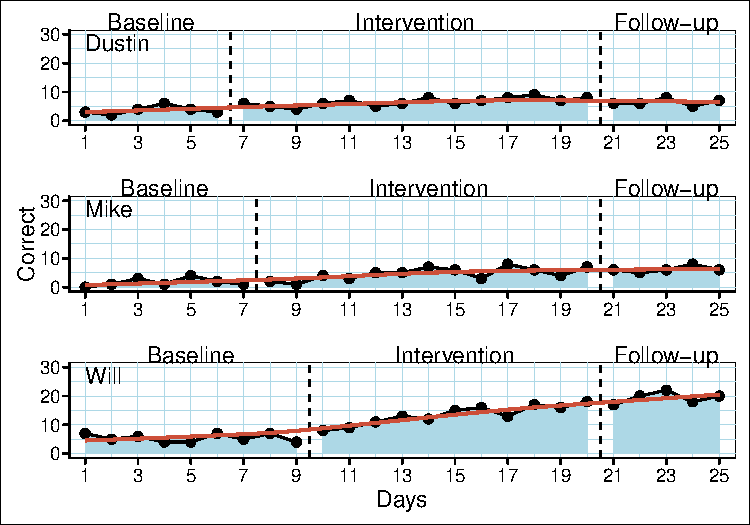
\includegraphics{./ch_introduction_files/figure-pdf/plot-strange-study-1.pdf}

}

\end{figure}

Now we need some descriptive statistics:

\begin{Shaded}
\begin{Highlighting}[]
\FunctionTok{describe}\NormalTok{(strange\_study)}
\end{Highlighting}
\end{Shaded}

\begin{longtable}[]{@{}lccc@{}}
\caption{Descriptive statistics}\tabularnewline
\toprule()
Parameter & Dustin & Mike & Will \\
\midrule()
\endfirsthead
\toprule()
Parameter & Dustin & Mike & Will \\
\midrule()
\endhead
Design & A-B-C & A-B-C & A-B-C \\
n A & 6 & 7 & 9 \\
n B & 14 & 13 & 11 \\
n C & 5 & 5 & 5 \\
Missing A & 0 & 0 & 0 \\
Missing B & 0 & 0 & 0 \\
Missing C & 0 & 0 & 0 \\
m A & 3.67 & 1.71 & 5.44 \\
m B & 6.57 & 4.69 & 13.45 \\
m C & 6.4 & 6.2 & 19.4 \\
md A & 3.5 & 1.0 & 5.0 \\
md B & 6.5 & 5.0 & 13.0 \\
md C & 6 & 6 & 20 \\
sd A & 1.37 & 1.38 & 1.33 \\
sd B & 1.40 & 2.10 & 3.27 \\
sd C & 1.14 & 1.10 & 1.95 \\
mad A & 0.74 & 1.48 & 1.48 \\
mad B & 1.48 & 2.97 & 4.45 \\
mad C & 1.48 & 0.00 & 2.97 \\
Min A & 2 & 0 & 4 \\
Min B & 4 & 1 & 8 \\
Min C & 5 & 5 & 17 \\
Max A & 6 & 4 & 7 \\
Max B & 9 & 8 & 18 \\
Max C & 8 & 8 & 22 \\
Trend A & 0.23 & 0.21 & -0.08 \\
Trend B & 0.25 & 0.36 & 0.91 \\
Trend C & 0.1 & 0.3 & 0.4 \\
{Note: } & & & \\
\textsuperscript{} n = Number of measurements; Missing = Number of
missing values; M = Mean; Median = Median; SD = Standard deviation; MAD
= Median average deviation; Min = Minimum; Max = Maximum; Trend = Slope
of dependent variable regressed on measurement-time. & & & \\
\bottomrule()
\end{longtable}

Single-case data are oftentimes analyzed with overlap indices. Let us
get an overview comparing phases A and B:

\begin{Shaded}
\begin{Highlighting}[]
\FunctionTok{overlap}\NormalTok{(strange\_study)}
\end{Highlighting}
\end{Shaded}

\begin{longtable}[]{@{}llll@{}}
\caption{Overlap indices. Comparing phase 1 against phase
2}\tabularnewline
\toprule()
& Dustin & Mike & Will \\
\midrule()
\endfirsthead
\toprule()
& Dustin & Mike & Will \\
\midrule()
\endhead
Design & A-B-C & A-B-C & A-B-C \\
PND & 50.00 & 53.85 & 100.00 \\
PEM & 100.00 & 92.31 & 100.00 \\
PET & 71.43 & 61.54 & 100.00 \\
NAP & 92.86 & 87.91 & 100.00 \\
NAP-R & 85.71 & 75.82 & 100.00 \\
PAND & 90 & 80 & 100 \\
Tau-U & 0.66 & 0.56 & 0.80 \\
Base Tau & 0.60 & 0.55 & 0.74 \\
Delta M & 2.90 & 2.98 & 8.01 \\
Delta Trend & 0.02 & 0.14 & 0.99 \\
SMD & 2.13 & 2.16 & 6.01 \\
Hedges g & 2.00 & 1.51 & 2.96 \\
{Note: } & & & \\
\textsuperscript{} PND = Percentage Non-Overlapping Data; PEM =
Percentage Exceeding the Median; PET = Percentage Exceeding the Trend;
NAP = Nonoverlap of all pairs; NAP-R = NAP rescaled; PAND = Percentage
all nonoverlapping data;Tau U = Parker\textquotesingle s Tau-U; Base Tau
= Baseline corrected Tau; Delta M = Mean difference between phases;
Delta Trend = Trend difference between phases; SMD = Standardized Mean
Difference; Hedges g = Corrected SMD. & & & \\
\bottomrule()
\end{longtable}

How do the changes hold up against the follow-up? Let us compare phases
A and C:

\begin{Shaded}
\begin{Highlighting}[]
\FunctionTok{overlap}\NormalTok{(strange\_study, }\AttributeTok{phases =} \FunctionTok{c}\NormalTok{(}\StringTok{"A"}\NormalTok{, }\StringTok{"C"}\NormalTok{))}
\end{Highlighting}
\end{Shaded}

\begin{longtable}[]{@{}llll@{}}
\caption{Overlap indices. Comparing phase A against phase
C}\tabularnewline
\toprule()
& Dustin & Mike & Will \\
\midrule()
\endfirsthead
\toprule()
& Dustin & Mike & Will \\
\midrule()
\endhead
Design & A-B-C & A-B-C & A-B-C \\
PND & 40 & 100 & 100 \\
PEM & 100 & 100 & 100 \\
PET & 0 & 60 & 100 \\
NAP & 93.33 & 100.00 & 100.00 \\
NAP-R & 86.67 & 100.00 & 100.00 \\
PAND & 81.82 & 100.00 & 100.00 \\
Tau-U & 0.46 & 0.51 & 0.61 \\
Base Tau & 0.67 & 0.76 & 0.74 \\
Delta M & 2.73 & 4.49 & 13.96 \\
Delta Trend & -0.13 & 0.09 & 0.48 \\
SMD & 2.00 & 3.25 & 10.47 \\
Hedges g & 1.97 & 3.25 & 8.34 \\
{Note: } & & & \\
\textsuperscript{} PND = Percentage Non-Overlapping Data; PEM =
Percentage Exceeding the Median; PET = Percentage Exceeding the Trend;
NAP = Nonoverlap of all pairs; NAP-R = NAP rescaled; PAND = Percentage
all nonoverlapping data;Tau U = Parker\textquotesingle s Tau-U; Base Tau
= Baseline corrected Tau; Delta M = Mean difference between phases;
Delta Trend = Trend difference between phases; SMD = Standardized Mean
Difference; Hedges g = Corrected SMD. & & & \\
\bottomrule()
\end{longtable}

Finally, we conduct regression analyses for each cases with a piecewise
regression model:

\begin{Shaded}
\begin{Highlighting}[]
\FunctionTok{plm}\NormalTok{(strange\_study}\SpecialCharTok{$}\NormalTok{Dustin)}
\FunctionTok{plm}\NormalTok{(strange\_study}\SpecialCharTok{$}\NormalTok{Mike)}
\FunctionTok{plm}\NormalTok{(strange\_study}\SpecialCharTok{$}\NormalTok{Will)}
\end{Highlighting}
\end{Shaded}

\begin{longtable}[]{@{}
  >{\raggedright\arraybackslash}p{(\columnwidth - 14\tabcolsep) * \real{0.1250}}
  >{\raggedleft\arraybackslash}p{(\columnwidth - 14\tabcolsep) * \real{0.1250}}
  >{\raggedleft\arraybackslash}p{(\columnwidth - 14\tabcolsep) * \real{0.1250}}
  >{\raggedleft\arraybackslash}p{(\columnwidth - 14\tabcolsep) * \real{0.1250}}
  >{\raggedleft\arraybackslash}p{(\columnwidth - 14\tabcolsep) * \real{0.1250}}
  >{\raggedleft\arraybackslash}p{(\columnwidth - 14\tabcolsep) * \real{0.1250}}
  >{\raggedleft\arraybackslash}p{(\columnwidth - 14\tabcolsep) * \real{0.1250}}
  >{\raggedleft\arraybackslash}p{(\columnwidth - 14\tabcolsep) * \real{0.1250}}@{}}
\caption{Piecewise-regression model predicting variable
\textquotesingle values\textquotesingle{}}\tabularnewline
\toprule()
\multicolumn{2}{@{}>{\raggedright\arraybackslash}p{(\columnwidth - 14\tabcolsep) * \real{0.2500} + 2\tabcolsep}}{%
\begin{minipage}[b]{\linewidth}\raggedright
\end{minipage}} &
\multicolumn{2}{>{\centering\arraybackslash}p{(\columnwidth - 14\tabcolsep) * \real{0.2500} + 2\tabcolsep}}{%
\begin{minipage}[b]{\linewidth}\centering
CI(95\%)
\end{minipage}} &
\multicolumn{4}{>{\raggedleft\arraybackslash}p{(\columnwidth - 14\tabcolsep) * \real{0.5000} + 6\tabcolsep}@{}}{%
\begin{minipage}[b]{\linewidth}\raggedleft
\end{minipage}} \\
\begin{minipage}[b]{\linewidth}\raggedright
Parameter
\end{minipage} & \begin{minipage}[b]{\linewidth}\raggedleft
B
\end{minipage} & \begin{minipage}[b]{\linewidth}\raggedleft
2.5\%
\end{minipage} & \begin{minipage}[b]{\linewidth}\raggedleft
97.5\%
\end{minipage} & \begin{minipage}[b]{\linewidth}\raggedleft
SE
\end{minipage} & \begin{minipage}[b]{\linewidth}\raggedleft
t
\end{minipage} & \begin{minipage}[b]{\linewidth}\raggedleft
p
\end{minipage} & \begin{minipage}[b]{\linewidth}\raggedleft
Delta R²
\end{minipage} \\
\midrule()
\endfirsthead
\toprule()
\multicolumn{2}{@{}>{\raggedright\arraybackslash}p{(\columnwidth - 14\tabcolsep) * \real{0.2500} + 2\tabcolsep}}{%
\begin{minipage}[b]{\linewidth}\raggedright
\end{minipage}} &
\multicolumn{2}{>{\centering\arraybackslash}p{(\columnwidth - 14\tabcolsep) * \real{0.2500} + 2\tabcolsep}}{%
\begin{minipage}[b]{\linewidth}\centering
CI(95\%)
\end{minipage}} &
\multicolumn{4}{>{\raggedleft\arraybackslash}p{(\columnwidth - 14\tabcolsep) * \real{0.5000} + 6\tabcolsep}@{}}{%
\begin{minipage}[b]{\linewidth}\raggedleft
\end{minipage}} \\
\begin{minipage}[b]{\linewidth}\raggedright
Parameter
\end{minipage} & \begin{minipage}[b]{\linewidth}\raggedleft
B
\end{minipage} & \begin{minipage}[b]{\linewidth}\raggedleft
2.5\%
\end{minipage} & \begin{minipage}[b]{\linewidth}\raggedleft
97.5\%
\end{minipage} & \begin{minipage}[b]{\linewidth}\raggedleft
SE
\end{minipage} & \begin{minipage}[b]{\linewidth}\raggedleft
t
\end{minipage} & \begin{minipage}[b]{\linewidth}\raggedleft
p
\end{minipage} & \begin{minipage}[b]{\linewidth}\raggedleft
Delta R²
\end{minipage} \\
\midrule()
\endhead
Intercept & 3.10 & 1.46 & 4.73 & 0.83 & 3.72 & \textless.01 & \\
Trend mt & 0.23 & -0.31 & 0.77 & 0.28 & 0.83 & .41 & .01 \\
Level phase B & 0.50 & -1.89 & 2.90 & 1.22 & 0.41 & .68 & .00 \\
Level phase C & -1.47 & -11.11 & 8.17 & 4.92 & -0.30 & .76 & .00 \\
Slope phase B & 0.02 & -0.54 & 0.58 & 0.29 & 0.06 & .95 & .00 \\
Slope phase C & -0.13 & -1.02 & 0.77 & 0.46 & -0.28 & .78 & .00 \\
{Note: } & & & & & & & \\
\textsuperscript{} F(5, 19) = 7.88; p \textless.001; R² = 0.675;
Adjusted R² = 0.589 & & & & & & & \\
\bottomrule()
\end{longtable}

\begin{longtable}[]{@{}
  >{\raggedright\arraybackslash}p{(\columnwidth - 14\tabcolsep) * \real{0.1250}}
  >{\raggedleft\arraybackslash}p{(\columnwidth - 14\tabcolsep) * \real{0.1250}}
  >{\raggedleft\arraybackslash}p{(\columnwidth - 14\tabcolsep) * \real{0.1250}}
  >{\raggedleft\arraybackslash}p{(\columnwidth - 14\tabcolsep) * \real{0.1250}}
  >{\raggedleft\arraybackslash}p{(\columnwidth - 14\tabcolsep) * \real{0.1250}}
  >{\raggedleft\arraybackslash}p{(\columnwidth - 14\tabcolsep) * \real{0.1250}}
  >{\raggedleft\arraybackslash}p{(\columnwidth - 14\tabcolsep) * \real{0.1250}}
  >{\raggedleft\arraybackslash}p{(\columnwidth - 14\tabcolsep) * \real{0.1250}}@{}}
\caption{Piecewise-regression model predicting variable
\textquotesingle values\textquotesingle{}}\tabularnewline
\toprule()
\multicolumn{2}{@{}>{\raggedright\arraybackslash}p{(\columnwidth - 14\tabcolsep) * \real{0.2500} + 2\tabcolsep}}{%
\begin{minipage}[b]{\linewidth}\raggedright
\end{minipage}} &
\multicolumn{2}{>{\centering\arraybackslash}p{(\columnwidth - 14\tabcolsep) * \real{0.2500} + 2\tabcolsep}}{%
\begin{minipage}[b]{\linewidth}\centering
CI(95\%)
\end{minipage}} &
\multicolumn{4}{>{\raggedleft\arraybackslash}p{(\columnwidth - 14\tabcolsep) * \real{0.5000} + 6\tabcolsep}@{}}{%
\begin{minipage}[b]{\linewidth}\raggedleft
\end{minipage}} \\
\begin{minipage}[b]{\linewidth}\raggedright
Parameter
\end{minipage} & \begin{minipage}[b]{\linewidth}\raggedleft
B
\end{minipage} & \begin{minipage}[b]{\linewidth}\raggedleft
2.5\%
\end{minipage} & \begin{minipage}[b]{\linewidth}\raggedleft
97.5\%
\end{minipage} & \begin{minipage}[b]{\linewidth}\raggedleft
SE
\end{minipage} & \begin{minipage}[b]{\linewidth}\raggedleft
t
\end{minipage} & \begin{minipage}[b]{\linewidth}\raggedleft
p
\end{minipage} & \begin{minipage}[b]{\linewidth}\raggedleft
Delta R²
\end{minipage} \\
\midrule()
\endfirsthead
\toprule()
\multicolumn{2}{@{}>{\raggedright\arraybackslash}p{(\columnwidth - 14\tabcolsep) * \real{0.2500} + 2\tabcolsep}}{%
\begin{minipage}[b]{\linewidth}\raggedright
\end{minipage}} &
\multicolumn{2}{>{\centering\arraybackslash}p{(\columnwidth - 14\tabcolsep) * \real{0.2500} + 2\tabcolsep}}{%
\begin{minipage}[b]{\linewidth}\centering
CI(95\%)
\end{minipage}} &
\multicolumn{4}{>{\raggedleft\arraybackslash}p{(\columnwidth - 14\tabcolsep) * \real{0.5000} + 6\tabcolsep}@{}}{%
\begin{minipage}[b]{\linewidth}\raggedleft
\end{minipage}} \\
\begin{minipage}[b]{\linewidth}\raggedright
Parameter
\end{minipage} & \begin{minipage}[b]{\linewidth}\raggedleft
B
\end{minipage} & \begin{minipage}[b]{\linewidth}\raggedleft
2.5\%
\end{minipage} & \begin{minipage}[b]{\linewidth}\raggedleft
97.5\%
\end{minipage} & \begin{minipage}[b]{\linewidth}\raggedleft
SE
\end{minipage} & \begin{minipage}[b]{\linewidth}\raggedleft
t
\end{minipage} & \begin{minipage}[b]{\linewidth}\raggedleft
p
\end{minipage} & \begin{minipage}[b]{\linewidth}\raggedleft
Delta R²
\end{minipage} \\
\midrule()
\endhead
Intercept & 1.07 & -0.95 & 3.09 & 1.03 & 1.04 & .31 & \\
Trend mt & 0.21 & -0.35 & 0.78 & 0.29 & 0.75 & .46 & .01 \\
Level phase B & -0.02 & -2.97 & 2.93 & 1.51 & -0.01 & .98 & .00 \\
Level phase C & 0.24 & -9.63 & 10.12 & 5.04 & 0.05 & .96 & .00 \\
Slope phase B & 0.14 & -0.46 & 0.75 & 0.31 & 0.46 & .64 & .00 \\
Slope phase C & 0.09 & -1.01 & 1.18 & 0.56 & 0.15 & .87 & .00 \\
{Note: } & & & & & & & \\
\textsuperscript{} F(5, 19) = 8.00; p \textless.001; R² = 0.678;
Adjusted R² = 0.593 & & & & & & & \\
\bottomrule()
\end{longtable}

\begin{longtable}[]{@{}
  >{\raggedright\arraybackslash}p{(\columnwidth - 14\tabcolsep) * \real{0.1250}}
  >{\raggedleft\arraybackslash}p{(\columnwidth - 14\tabcolsep) * \real{0.1250}}
  >{\raggedleft\arraybackslash}p{(\columnwidth - 14\tabcolsep) * \real{0.1250}}
  >{\raggedleft\arraybackslash}p{(\columnwidth - 14\tabcolsep) * \real{0.1250}}
  >{\raggedleft\arraybackslash}p{(\columnwidth - 14\tabcolsep) * \real{0.1250}}
  >{\raggedleft\arraybackslash}p{(\columnwidth - 14\tabcolsep) * \real{0.1250}}
  >{\raggedleft\arraybackslash}p{(\columnwidth - 14\tabcolsep) * \real{0.1250}}
  >{\raggedleft\arraybackslash}p{(\columnwidth - 14\tabcolsep) * \real{0.1250}}@{}}
\caption{Piecewise-regression model predicting variable
\textquotesingle values\textquotesingle{}}\tabularnewline
\toprule()
\multicolumn{2}{@{}>{\raggedright\arraybackslash}p{(\columnwidth - 14\tabcolsep) * \real{0.2500} + 2\tabcolsep}}{%
\begin{minipage}[b]{\linewidth}\raggedright
\end{minipage}} &
\multicolumn{2}{>{\centering\arraybackslash}p{(\columnwidth - 14\tabcolsep) * \real{0.2500} + 2\tabcolsep}}{%
\begin{minipage}[b]{\linewidth}\centering
CI(95\%)
\end{minipage}} &
\multicolumn{4}{>{\raggedleft\arraybackslash}p{(\columnwidth - 14\tabcolsep) * \real{0.5000} + 6\tabcolsep}@{}}{%
\begin{minipage}[b]{\linewidth}\raggedleft
\end{minipage}} \\
\begin{minipage}[b]{\linewidth}\raggedright
Parameter
\end{minipage} & \begin{minipage}[b]{\linewidth}\raggedleft
B
\end{minipage} & \begin{minipage}[b]{\linewidth}\raggedleft
2.5\%
\end{minipage} & \begin{minipage}[b]{\linewidth}\raggedleft
97.5\%
\end{minipage} & \begin{minipage}[b]{\linewidth}\raggedleft
SE
\end{minipage} & \begin{minipage}[b]{\linewidth}\raggedleft
t
\end{minipage} & \begin{minipage}[b]{\linewidth}\raggedleft
p
\end{minipage} & \begin{minipage}[b]{\linewidth}\raggedleft
Delta R²
\end{minipage} \\
\midrule()
\endfirsthead
\toprule()
\multicolumn{2}{@{}>{\raggedright\arraybackslash}p{(\columnwidth - 14\tabcolsep) * \real{0.2500} + 2\tabcolsep}}{%
\begin{minipage}[b]{\linewidth}\raggedright
\end{minipage}} &
\multicolumn{2}{>{\centering\arraybackslash}p{(\columnwidth - 14\tabcolsep) * \real{0.2500} + 2\tabcolsep}}{%
\begin{minipage}[b]{\linewidth}\centering
CI(95\%)
\end{minipage}} &
\multicolumn{4}{>{\raggedleft\arraybackslash}p{(\columnwidth - 14\tabcolsep) * \real{0.5000} + 6\tabcolsep}@{}}{%
\begin{minipage}[b]{\linewidth}\raggedleft
\end{minipage}} \\
\begin{minipage}[b]{\linewidth}\raggedright
Parameter
\end{minipage} & \begin{minipage}[b]{\linewidth}\raggedleft
B
\end{minipage} & \begin{minipage}[b]{\linewidth}\raggedleft
2.5\%
\end{minipage} & \begin{minipage}[b]{\linewidth}\raggedleft
97.5\%
\end{minipage} & \begin{minipage}[b]{\linewidth}\raggedleft
SE
\end{minipage} & \begin{minipage}[b]{\linewidth}\raggedleft
t
\end{minipage} & \begin{minipage}[b]{\linewidth}\raggedleft
p
\end{minipage} & \begin{minipage}[b]{\linewidth}\raggedleft
Delta R²
\end{minipage} \\
\midrule()
\endhead
Intercept & 5.78 & 3.96 & 7.59 & 0.93 & 6.23 & \textless.001 & \\
Trend mt & -0.08 & -0.46 & 0.30 & 0.19 & -0.43 & .67 & .00 \\
Level phase B & 3.88 & 1.16 & 6.60 & 1.39 & 2.80 & \textless.05 & .02 \\
Level phase C & 14.49 & 7.89 & 21.08 & 3.37 & 4.31 & \textless.001 &
.05 \\
Slope phase B & 0.99 & 0.52 & 1.47 & 0.24 & 4.10 & \textless.001 &
.05 \\
Slope phase C & 0.48 & -0.53 & 1.49 & 0.52 & 0.94 & .35 & .00 \\
{Note: } & & & & & & & \\
\textsuperscript{} F(5, 19) = 68.16; p \textless.001; R² = 0.947;
Adjusted R² = 0.933 & & & & & & & \\
\bottomrule()
\end{longtable}

\hypertarget{some-things-about-r}{%
\chapter{Some things about R}\label{some-things-about-r}}

In this chapter you will get a brief introduction to R. If you are
familiar with R you might like to go directly to the next chapter.

\hfill\break
R is a programming language optimized for statistical purposes. It was
created in 1992 by Ross Ihaka and Robert Gentleman at the University of
Auckland. Since then it has been developed continuously and became one
of the leading statistical software programs. R is unmatched in its
versatility. It is used for teaching introductory courses into
statistics up to doing the most sophisticated mathematical analysis. It
has become the defacto standard in many scientific disciplines from the
natural to the social sciences.\\
R is completely community driven . That is, it is developed and extended
by anybody who likes to participate . It comes at no costs and can be
downloaded for free for all major and many minor platforms at
\href{http://www.r-project.org}{www.r-project.org}. Yet, it is as
reliable as other proprietary software like Mplus, STATA, SPSS etc . You
can tell from my writing that is hard not to become an R-fan when you
are into statistics :-)\\
R can be used in at least two ways:

\begin{enumerate}
\def\labelenumi{\arabic{enumi}.}
\tightlist
\item
  You can use it for applying data analyses. In that way it functions
  like most other statistical programs. You have to learn the specific
  syntax of R and it will compute the data analysis you need. For
  example \texttt{mean(x)} will return the mean of the variable
  \texttt{x}; \texttt{lm(y\ \textasciitilde{}\ x)} will calculate a
  linear regression with the criteria \texttt{y} and the predictor
  \texttt{x} for you or \texttt{plot(x,\ y)} will return a scatter-plot
  of the variables \texttt{x} and \texttt{y}.
\item
  You can use R to program new statistical procedures, or extend
  previous ones.
\end{enumerate}

It is the second function that is the origin of R's huge success and
versatility. New statistical procedures and functions can be published
to be used for everyone in so called packages. A package usually
contains several functions, help files and example data-sets. Hundreds
of such packages are available to help in all kinds of specialized
analyses. The basic installation of R comes with a large variety of
packages per installed. New packages can most of the times be easily
installed from within R. Admittedly, if you must have the latest
developmental version of a new package installation sometimes can get a
bit more complex. But with a bit of help and persistence it is not to
difficult to accomplish.

The book at hand describes the use of such an additional package named
\emph{scan} providing specialized functions for single-case analyses.
\emph{scan} comes in two versions: A ``stable'' version and a
developmental version. Both versions can be installed directly from
within R. The stable version is much older and only provides a limited
functionality. Therefore, I will refer to the developmental version in
this book.

\hypertarget{basic-r}{%
\section{Basic R}\label{basic-r}}

\emph{R} is a script language. That is, you type in text and let R
execute the commands you wrote down. Either you work in a \emph{console}
or a \emph{textfile}. In a \emph{console} the command will be executed
every time you press the RETURN-key. In a \emph{textfile} you type down
your code, mark the part you like to be executed, and run that code
(with a click or a certain key). The latter text files can be saved and
reused for later R sessions. Therefore, usually you will work in a text
file.

A value is assigned to a variable with the \texttt{\textless{}-}
operator. Which should be read as an arrow rather than a less sign and a
minus sign. A \texttt{\#} is followed by a comment to make your code
more understandable. So, what follows a \texttt{\#} is not interpreted
by R. A vector is a chain of several values. With a vector you could
describe the values of a measurement series. The \texttt{c} function is
used to build a vector (e.g., \texttt{c(1,\ 2,\ 3,\ 4)}). If you like to
see the content of a variable you could use the \texttt{print} function.
\texttt{print(x)} will display the content of the variable \texttt{x}. A
shortcut for this is just to type variable name (and press return)
\texttt{x}.

\begin{Shaded}
\begin{Highlighting}[]
\CommentTok{\# x is assigned the value 10:}
\NormalTok{x }\OtherTok{\textless{}{-}} \DecValTok{10}

\CommentTok{\# See what\textquotesingle{}s inside of x:}
\NormalTok{x}
\end{Highlighting}
\end{Shaded}

\begin{verbatim}
[1] 10
\end{verbatim}

\begin{Shaded}
\begin{Highlighting}[]
\CommentTok{\# x is assigned a vector with three values:}
\NormalTok{x }\OtherTok{\textless{}{-}} \FunctionTok{c}\NormalTok{(}\DecValTok{10}\NormalTok{, }\DecValTok{11}\NormalTok{, }\DecValTok{15}\NormalTok{)}

\CommentTok{\# ... and display the content of x:}
\NormalTok{x}
\end{Highlighting}
\end{Shaded}

\begin{verbatim}
[1] 10 11 15
\end{verbatim}

Two important concepts in \textbf{R} are \emph{functions} and
\emph{arguments}. A \emph{function} is the name for a procedure that
does something with the \emph{arguments} that are provided by you. For
example, the function \texttt{mean} calculated the mean. \texttt{mean}
has an argument \texttt{x} which ``expects'' that you provide a vector
(a series of values) from which it will calculate the mean.
\texttt{mean(\ x\ =\ c(1,\ 3,\ 5)\ )} will compute the mean of the
values 1, 3, and 5 and return the result 3. Some \emph{functions} can
take several arguments. \texttt{mean} for example also takes the
argument \texttt{trim}. For calculating a trimmed mean.
\texttt{mean(\ x\ =\ c(1,\ 1,\ 3,\ 3,\ 5,\ 6,\ 7,\ 8,\ 9,\ 9),\ trim\ =\ 0.1)}
will calculate the 10\% trimmed mean of the provided values. The name of
the first argument could be dropped. That is,
\texttt{mean(\ c(1,\ 3,\ 5)\ )} will be interpreted by \textbf{R} as
\texttt{mean(\ x\ =\ c(1,\ 3,\ 5)\ )}. You could also provide a variable
to an argument.

\begin{Shaded}
\begin{Highlighting}[]
\NormalTok{values }\OtherTok{\textless{}{-}} \FunctionTok{c}\NormalTok{(}\DecValTok{1}\NormalTok{, }\DecValTok{4}\NormalTok{, }\DecValTok{5}\NormalTok{, }\DecValTok{6}\NormalTok{, }\DecValTok{3}\NormalTok{, }\DecValTok{7}\NormalTok{, }\DecValTok{7}\NormalTok{, }\DecValTok{5}\NormalTok{)}
\FunctionTok{mean}\NormalTok{(}\AttributeTok{x =}\NormalTok{ values)}
\end{Highlighting}
\end{Shaded}

\begin{verbatim}
[1] 4.75
\end{verbatim}

\begin{Shaded}
\begin{Highlighting}[]
\CommentTok{\# or shorter:}
\FunctionTok{mean}\NormalTok{(values)}
\end{Highlighting}
\end{Shaded}

\begin{verbatim}
[1] 4.75
\end{verbatim}

The return value of a function can be assigned to a new variable
instead:

\begin{Shaded}
\begin{Highlighting}[]
\NormalTok{y }\OtherTok{\textless{}{-}} \FunctionTok{c}\NormalTok{(}\DecValTok{1}\NormalTok{, }\DecValTok{4}\NormalTok{, }\DecValTok{5}\NormalTok{, }\DecValTok{6}\NormalTok{, }\DecValTok{3}\NormalTok{, }\DecValTok{7}\NormalTok{, }\DecValTok{7}\NormalTok{, }\DecValTok{5}\NormalTok{)}
\NormalTok{res }\OtherTok{\textless{}{-}} \FunctionTok{mean}\NormalTok{(y)}
\CommentTok{\#now res contains the mean of y:}
\NormalTok{res}
\end{Highlighting}
\end{Shaded}

\begin{verbatim}
[1] 4.75
\end{verbatim}

Every function in R has a help page written by the programmers. You can
retrieve these pages with the \texttt{help} function or the short cut
\texttt{?}. \texttt{help("mean")} will display the help page for the
\texttt{mean} function. The quotation marks are necessary here because
you do not provide a variable with the name \emph{mean} but a word
`mean'. The shortcut works \texttt{?mean}. A bit confusingly, you do not
need the quotation marks here.

\hypertarget{the-scan-package}{%
\chapter{The scan package}\label{the-scan-package}}

\hypertarget{installing-the-scan-package}{%
\section{\texorpdfstring{Installing the \emph{scan}
package}{Installing the scan package}}\label{installing-the-scan-package}}

You can use the \texttt{install.packages} function to install
\emph{scan}.

\texttt{install.packages("scan")} will install the stable version.

The current stable release is version \texttt{0.55}. Please look at
Section \emph{Software reference} for which version of \emph{scan} has
been used for creating this book and make sure you have this version or
a newer one installed.

R contains many packages and it would significantly slow down if all
packages would be loaded into the computer memory at the beginning of
each R session. Therefore, after installing \emph{scan} it needs to be
activated at the beginning of each session you use R. Usually a session
starts when you start the R program and ends with closing R.

For activating a package you need the \texttt{library} function. In this
case \texttt{library(scan)}. You should get something like

\begin{verbatim}
scan 0.55.1 (2022-09-09)
Single-Case Data Analysis for Single and Multiple Baseline Designs
\end{verbatim}

indicating that everything went smoothly and \emph{scan} is ready for
the job.

\hypertarget{development-version-of-scan}{%
\section{Development version of
scan}\label{development-version-of-scan}}

Alternatively, you can compile the development version of \emph{scan}
yourself. This might be necessary if the stable version has some bugs or
missing functions which has been fixed.

You may need some computer expertise to get the development version
running. It is hosted on gitHub at
\href{https://github.com/jazznbass/scan}{\textless https://github.com/jazznbass/scan\textgreater{}}.

For installation, you can apply the \texttt{install\_github} function
from the \texttt{devtools} package (make sure you have installed the
\texttt{devtools} package before):

\texttt{devtools::install\_github("jazznbass/scan",\ dependencies\ =\ TRUE)}

When you are running a Windows operating system you will probably have
to install Rtools before. Rtools contains additional programs
(e.g.~compilers) that are needed to compile R source packages.

You can find Rtools here:
\href{https://cran.r-project.org/bin/windows/Rtools/}{\textless https://cran.r-project.org/bin/windows/Rtools/\textgreater{}}

\hypertarget{reporting-issues-with-scan-and-suggesting-enhancements}{%
\section{\texorpdfstring{Reporting issues with \emph{scan} and
suggesting
enhancements}{Reporting issues with scan and suggesting enhancements}}\label{reporting-issues-with-scan-and-suggesting-enhancements}}

The \emph{scan} gitHub repository at
\href{https://github.com/jazznbass/scan}{\textless https://github.com/jazznbass/scan\textgreater{}}
is the ideal place to report bugs, problems, or ideas for enhancing
\emph{scan}. Please use the issue tool (direct link:
\href{https://github.com/jazznbass/scan/issues}{\textless https://github.com/jazznbass/scan/issues\textgreater{}}).

We are very thankful for any feedback, corrections, or whatever helps to
improve \emph{scan}!

\hypertarget{functions-overview}{%
\section{Functions overview}\label{functions-overview}}

The functions of the \emph{scan} package can be divided into the
following categories:\\
\emph{Manage data}, \emph{analyze}, \emph{manipulate}, \emph{simulate},
and \emph{depict}.

The following tables give an overview of all functions. Furthermore, you
can see the current life cycle stage of a function. The life cycle stage
categorization is based on the tidyverse package and described in detail
here https://lifecycle.r-lib.org/articles/stages.html.

\hypertarget{management}{%
\subsection{Management}\label{management}}

\hypertarget{tbl-functions-management}{}
\begin{longtable}[]{@{}
  >{\raggedright\arraybackslash}p{(\columnwidth - 6\tabcolsep) * \real{0.2500}}
  >{\raggedright\arraybackslash}p{(\columnwidth - 6\tabcolsep) * \real{0.4773}}
  >{\raggedright\arraybackslash}p{(\columnwidth - 6\tabcolsep) * \real{0.1212}}
  >{\raggedright\arraybackslash}p{(\columnwidth - 6\tabcolsep) * \real{0.1515}}@{}}
\caption{\label{tbl-functions-management}Functions for data
management}\tabularnewline
\toprule()
\begin{minipage}[b]{\linewidth}\raggedright
Function
\end{minipage} & \begin{minipage}[b]{\linewidth}\raggedright
What it does \ldots{}
\end{minipage} & \begin{minipage}[b]{\linewidth}\raggedright
Lifecycle stage
\end{minipage} & \begin{minipage}[b]{\linewidth}\raggedright
Chapter
\end{minipage} \\
\midrule()
\endfirsthead
\toprule()
\begin{minipage}[b]{\linewidth}\raggedright
Function
\end{minipage} & \begin{minipage}[b]{\linewidth}\raggedright
What it does \ldots{}
\end{minipage} & \begin{minipage}[b]{\linewidth}\raggedright
Lifecycle stage
\end{minipage} & \begin{minipage}[b]{\linewidth}\raggedright
Chapter
\end{minipage} \\
\midrule()
\endhead
scdf & Creates a single-case data-frame & Stable &
Section~\ref{sec-scdf} \\
select\_cases & Selects specific cases of an scdf & Stable &
Section~\ref{sec-select-cases}) \\
select\_phases & Selects and/or recombines phases & Stable &
Section~\ref{sec-select-phases}) \\
subset & Selects specific measurements or variables of an scdf & stable
& Section~\ref{sec-subset} \\
read\_scdf & Loads external data into an scdf & Stable &
Section~\ref{sec-read-scdf}) \\
write\_scdf & Writes scdf into an external file & Stable &
Section~\ref{sec-write-scdf}) \\
convert & Converts an scdf object into R syntax & Stable &
Section~\ref{sec-convert} \\
set\_var & (Re)sets dependent, measurement, and phase variable of an
scdf & Stable & - \\
scdf\_attr & Gets and sets attributes of an scdf & Stable & - \\
add\_l2 & Adds level-two data to an scdf & Stable &
Section~\ref{sec-add-l2}) \\
as.data.frame/as.data.frame.scdf & Transforms an scdf into a data frame
& Stable & - \\
\bottomrule()
\end{longtable}

\hypertarget{depiction}{%
\subsection{Depiction}\label{depiction}}

\hypertarget{tbl-functions-depiction}{}
\begin{longtable}[]{@{}lll@{}}
\caption{\label{tbl-functions-depiction}Functions for data
depiction/visualisation}\tabularnewline
\toprule()
Function & What it does ... & Lifecycle stage \\
\midrule()
\endfirsthead
\toprule()
Function & What it does ... & Lifecycle stage \\
\midrule()
\endhead
plot/plot.scdf & Creates plots of single cases & Superseded \\
scplot & Add-on package `scplot`. Create advanced ggplot2 plots. &
Experimental \\
style\_plot & Defines single-case plot graphical styles & Superseded \\
export & Creates html or latex tables from the output of various can
functions & Experimental \\
print/print.sc & Prints the results of various scan outputs & Stable \\
print/print.scdf & Prints an scdf & Stable \\
summary/summary.scdf & Summaizes an scdf & Stable \\
plot\_rand & Create a distribution plot from a randomization test obejct
& Experimental \\
\bottomrule()
\end{longtable}

\hypertarget{analysis}{%
\subsection{Analysis}\label{analysis}}

\hypertarget{tbl-functions-analysis}{}
\begin{longtable}[]{@{}lll@{}}
\caption{\label{tbl-functions-analysis}Functions for data
analysis}\tabularnewline
\toprule()
Function & What it does ... & Lifecycle stage \\
\midrule()
\endfirsthead
\toprule()
Function & What it does ... & Lifecycle stage \\
\midrule()
\endhead
autocorr & Autocorrelations for each phase of each case & Stable \\
corrected\_tau & Baseline corrected tau & Stable \\
describe & Descriptive statistics for each phase of each case &
Stable \\
overlap & An overview of overlap indeces for each case & Stable \\
smd & Various standardized mean differences between phase A and B &
Stable \\
rci & Reliable change index & Experimental \\
rand\_test & Randomization test & Stable \\
tau\_u & Tau-U for each case and all cases & Stable \\
trend & Trend analyses for each case & Stable \\
plm & Piecewise linear regression model & Stable \\
mplm & Multivariate piecewise linear regression model & Experimental \\
hplm & Hierarchical piecewise linear regression model & Stable \\
nap & Non-overlap of all pairs for each case & Stable \\
pnd & Percentage of non overlapping data for each case & Stable \\
pand & Percentage of all non overlapping data for all cases & Stable \\
pem & Percantage exceeding the mean for each case & Stable \\
pet & Percentage exceeding the trend for each case & Stable \\
cdc & Conservative dual-criterion test & Stable \\
outlier & Detect outliers for all cases & Stable \\
\bottomrule()
\end{longtable}

\hypertarget{manipulation}{%
\subsection{Manipulation}\label{manipulation}}

\hypertarget{tbl-functions-manipulation}{}
\begin{longtable}[]{@{}lll@{}}
\caption{\label{tbl-functions-manipulation}Functions for data
manipulation}\tabularnewline
\toprule()
Function & What it does ... & Lifecycle stage \\
\midrule()
\endfirsthead
\toprule()
Function & What it does ... & Lifecycle stage \\
\midrule()
\endhead
fill\_missing & Interpolate missign values or missing measurement times
& Stable \\
ranks & Covert data into ranked data across all cases & Stable \\
transform & Change and create new variabes & Stable \\
smooth\_cases & Smoothes time series data & Stable \\
truncate\_phase & Deletes measurements of phases & Stable \\
standardize & Standardizes or centers variables across cases & Stable \\
\bottomrule()
\end{longtable}

\hypertarget{simulation}{%
\subsection{Simulation}\label{simulation}}

\hypertarget{tbl-functions-simulation}{}
\begin{longtable}[]{@{}lll@{}}
\caption{\label{tbl-functions-simulation}Functions for data
simulation}\tabularnewline
\toprule()
Function & What it does ... & Lifecycle stage \\
\midrule()
\endfirsthead
\toprule()
Function & What it does ... & Lifecycle stage \\
\midrule()
\endhead
design & Defines a design of one or multiple single-cases & Stable \\
power\_test & Calculates power and alpha error of a specific analyzes
for a specific single-case design & Stable \\
estimate\_design & Extraxt a deisgn template from an existing scdf &
Experimental \\
random\_scdf & Creats random single-case studies from a single-case
design & Stable \\
mcscan & Add-on package `mcscan`. Create Monte-Carlo designs and
analyses with `scan` & (Upcoming not yet functioning) \\
\bottomrule()
\end{longtable}

\hypertarget{managing-single-case-data}{%
\chapter{Managing single-case data}\label{managing-single-case-data}}

\hypertarget{a-single-case-data-frame}{%
\section{\texorpdfstring{A \textbf{\emph{single-case data
frame}}}{A single-case data frame}}\label{a-single-case-data-frame}}

Scan provides its own data-class for encoding single-case data: the
\emph{single-case data frame} (short \emph{scdf}). An \emph{scdf} is an
object that contains one or multiple single-case data sets and is
optimized for managing and displaying these data. Think of an scdf as a
file including a separate datasheet for each single case. Each datasheet
is made up of at least three variables: The measured \textbf{values},
the \textbf{phase} identifier for each measured value, and the
measurement time (\textbf{mt}) of each measure. Optionally, scdfs could
include further variables for each single-case (e.g., control
variables), and also a name for each case.

\begin{tcolorbox}[enhanced jigsaw, opacitybacktitle=0.6, breakable, bottomrule=.15mm, coltitle=black, colbacktitle=quarto-callout-note-color!10!white, colframe=quarto-callout-note-color-frame, left=2mm, colback=white, titlerule=0mm, leftrule=.75mm, opacityback=0, toptitle=1mm, title=\textcolor{quarto-callout-note-color}{\faInfo}\hspace{0.5em}{Note}, arc=.35mm, rightrule=.15mm, toprule=.15mm, bottomtitle=1mm]
Technically, an scdf object is a list containing data frames. It is of
the class \texttt{c("scdf","list")}. Additionally, an \emph{scdf}
entails an attribute \texttt{scdf} with a list with further attributes.
\texttt{var.values}, \texttt{var.phase}, and \texttt{var.mt} contain the
names of the \texttt{values}, \texttt{phase}, and the
\texttt{measurement\ time} variable. By default, these names are set to
\texttt{values}, \texttt{phase}, and \texttt{mt}.
\end{tcolorbox}

Several functions are available for creating, transforming, merging, and
importing/exporting \emph{scdfs}.

\hypertarget{sec-scdf}{%
\section{Creating scdfs}\label{sec-scdf}}

\begin{tcolorbox}[enhanced jigsaw, toprule=.15mm, colframe=quarto-callout-tip-color-frame, left=2mm, colback=white, breakable, bottomrule=.15mm, arc=.35mm, rightrule=.15mm, leftrule=.75mm, opacityback=0]
\begin{minipage}[t]{5.5mm}
\textcolor{quarto-callout-tip-color}{\faLightbulb}
\end{minipage}%
\begin{minipage}[t]{\textwidth - 5.5mm}
scdf(values, B\_start, mt, phase, phase\_design = NULL, name = NULL,
dvar = ``values'', pvar = ``phase'', mvar = ``mt'',
\ldots)\end{minipage}%
\end{tcolorbox}

The \texttt{scdf} function is the basic tool for creating a single-case
data frame. Basically, you have to provide the measurement \emph{values}
and the \emph{phase} structure and a scdf object is build. There are
three different ways of defining the phase structure. First, defining
the beginning of the B-phase with the \texttt{B\_start} argument,
second, defining a design with the \texttt{phase\_design} argument and
third, setting parameters in a named vector of the dependent variable.

\begin{Shaded}
\begin{Highlighting}[]
\DocumentationTok{\#\#\# Three ways to code the same scdf}
\FunctionTok{scdf}\NormalTok{(}\AttributeTok{values =} \FunctionTok{c}\NormalTok{(}\AttributeTok{A =} \DecValTok{2}\NormalTok{,}\DecValTok{2}\NormalTok{,}\DecValTok{4}\NormalTok{,}\DecValTok{5}\NormalTok{, }\AttributeTok{B =} \DecValTok{8}\NormalTok{,}\DecValTok{7}\NormalTok{,}\DecValTok{6}\NormalTok{,}\DecValTok{9}\NormalTok{,}\DecValTok{8}\NormalTok{,}\DecValTok{7}\NormalTok{))}
\FunctionTok{scdf}\NormalTok{(}\AttributeTok{values =} \FunctionTok{c}\NormalTok{(}\DecValTok{2}\NormalTok{,}\DecValTok{2}\NormalTok{,}\DecValTok{4}\NormalTok{,}\DecValTok{5}\NormalTok{,}\DecValTok{8}\NormalTok{,}\DecValTok{7}\NormalTok{,}\DecValTok{6}\NormalTok{,}\DecValTok{9}\NormalTok{,}\DecValTok{8}\NormalTok{,}\DecValTok{7}\NormalTok{), }\AttributeTok{B\_start =} \DecValTok{5}\NormalTok{)}
\FunctionTok{scdf}\NormalTok{(}\AttributeTok{values =} \FunctionTok{c}\NormalTok{(}\DecValTok{2}\NormalTok{,}\DecValTok{2}\NormalTok{,}\DecValTok{4}\NormalTok{,}\DecValTok{5}\NormalTok{,}\DecValTok{8}\NormalTok{,}\DecValTok{7}\NormalTok{,}\DecValTok{6}\NormalTok{,}\DecValTok{9}\NormalTok{,}\DecValTok{8}\NormalTok{,}\DecValTok{7}\NormalTok{), }\AttributeTok{phase\_design =} \FunctionTok{c}\NormalTok{(}\AttributeTok{A =} \DecValTok{4}\NormalTok{, }\AttributeTok{B =} \DecValTok{6}\NormalTok{))}
\end{Highlighting}
\end{Shaded}

The \texttt{B\_start} argument is only applicable when the single-case
consists of a single A-phase followed by a B-phase. It is a remnant from
the time when \texttt{scan} could only handle sign-case designs with two
phases. The number assigned to \texttt{B\_start} indicates the
measurement-time as defined in the \texttt{mt} argument. That is, assume
a vector for the measurement times
\texttt{mt\ =\ c(1,3,7,10,15,17,18,20)} and \texttt{B\_start\ =\ 15}
then the first measurement of the B-phase will start with the fifth
measurement at which \emph{mt} = 15.\\
The \texttt{phase\_design} argument is a named vector with the name and
length of each phase. The phase names can be set arbitrary, although I
recommend to use capital letters (A, B, C, \ldots) for each phase
followed by, when indicated, a number if the phases repeat (A1, B1, A2,
B2, \ldots). Although it is possible to give the same name to more than
one phase (A, B, A, B) this might lead to some confusion and errors when
coding analyzes with \emph{scan}.\\
When the vector of the dependent variable includes named values, a
phase\_design structure is created automatically. Each named value sets
the beginning of a new phase. For example
\texttt{c(A\ =\ 3,2,4,\ B\ =\ 5,4,3,\ C\ =\ 6,7,6,5)} will create an
ABC-phase design with 3, 3, and 4 values per phase.\\
Use only one of the three methods at a time and I recommend to use the
\texttt{phase\_design} argument or the named vector method as they are
the most versatile.\\
If no measurement times are given, scdf automatically adds them numbered
sequentially 1, 2, 3, \ldots, \emph{N} where \emph{N} is the number of
measurements. in some circumstances it might be useful to define
individual measurement times for each measurement. For example, if you
want to include the days since the beginning of the study as time
intervals between measurements are widely varying you might get more
valid results this way when analyzing the data in a regression approach.

\begin{Shaded}
\begin{Highlighting}[]
\CommentTok{\# example of a more complex design }
\FunctionTok{scdf}\NormalTok{(}
  \AttributeTok{values =} \FunctionTok{c}\NormalTok{(}\DecValTok{2}\NormalTok{,}\DecValTok{2}\NormalTok{,}\DecValTok{4}\NormalTok{,}\DecValTok{5}\NormalTok{, }\DecValTok{8}\NormalTok{,}\DecValTok{7}\NormalTok{,}\DecValTok{6}\NormalTok{,}\DecValTok{9}\NormalTok{,}\DecValTok{8}\NormalTok{,}\DecValTok{7}\NormalTok{, }\DecValTok{12}\NormalTok{,}\DecValTok{11}\NormalTok{,}\DecValTok{13}\NormalTok{), }
  \AttributeTok{mt =} \FunctionTok{c}\NormalTok{(}\DecValTok{1}\NormalTok{,}\DecValTok{2}\NormalTok{,}\DecValTok{3}\NormalTok{,}\DecValTok{6}\NormalTok{, }\DecValTok{8}\NormalTok{,}\DecValTok{9}\NormalTok{,}\DecValTok{11}\NormalTok{,}\DecValTok{12}\NormalTok{,}\DecValTok{16}\NormalTok{,}\DecValTok{18}\NormalTok{, }\DecValTok{27}\NormalTok{,}\DecValTok{28}\NormalTok{,}\DecValTok{29}\NormalTok{),}
  \AttributeTok{phase\_design =} \FunctionTok{c}\NormalTok{(}\AttributeTok{A =} \DecValTok{4}\NormalTok{, }\AttributeTok{B =} \DecValTok{6}\NormalTok{, }\AttributeTok{C =} \DecValTok{3}\NormalTok{)}
\NormalTok{)}
\end{Highlighting}
\end{Shaded}

\begin{verbatim}
#A single-case data frame with one case

 Case1: values mt phase
             2  1     A
             2  2     A
             4  3     A
             5  6     A
             8  8     B
             7  9     B
             6 11     B
             9 12     B
             8 16     B
             7 18     B
            12 27     C
            11 28     C
            13 29     C
\end{verbatim}

Missing values could be coded using \texttt{NA} (not available).

\begin{Shaded}
\begin{Highlighting}[]
\FunctionTok{scdf}\NormalTok{(}\AttributeTok{values =} \FunctionTok{c}\NormalTok{(}\AttributeTok{A =} \DecValTok{2}\NormalTok{,}\DecValTok{2}\NormalTok{,}\ConstantTok{NA}\NormalTok{,}\DecValTok{5}\NormalTok{, }\AttributeTok{B =} \DecValTok{8}\NormalTok{,}\DecValTok{7}\NormalTok{,}\DecValTok{6}\NormalTok{,}\DecValTok{9}\NormalTok{,}\ConstantTok{NA}\NormalTok{,}\DecValTok{7}\NormalTok{))}
\end{Highlighting}
\end{Shaded}

More variables are implemented by adding new variable names with a
vector containing the values. Please be aware that a new variable must
never have the same name as one of the arguments of the function
(i.e.~B\_start, phase\_design, name, dvar, pvar, mvar).

\begin{Shaded}
\begin{Highlighting}[]
\FunctionTok{scdf}\NormalTok{(}
  \AttributeTok{values =} \FunctionTok{c}\NormalTok{(}\AttributeTok{A =} \DecValTok{2}\NormalTok{,}\DecValTok{2}\NormalTok{,}\DecValTok{3}\NormalTok{,}\DecValTok{5}\NormalTok{, }\AttributeTok{B =} \DecValTok{8}\NormalTok{,}\DecValTok{7}\NormalTok{,}\DecValTok{6}\NormalTok{,}\DecValTok{9}\NormalTok{,}\DecValTok{7}\NormalTok{,}\DecValTok{7}\NormalTok{), }
  \AttributeTok{teacher =} \FunctionTok{c}\NormalTok{(}\DecValTok{0}\NormalTok{,}\DecValTok{0}\NormalTok{,}\DecValTok{1}\NormalTok{,}\DecValTok{1}\NormalTok{,}\DecValTok{0}\NormalTok{,}\DecValTok{1}\NormalTok{,}\DecValTok{1}\NormalTok{,}\DecValTok{1}\NormalTok{,}\DecValTok{0}\NormalTok{,}\DecValTok{1}\NormalTok{), }
  \AttributeTok{hour =} \FunctionTok{c}\NormalTok{(}\DecValTok{2}\NormalTok{,}\DecValTok{3}\NormalTok{,}\DecValTok{4}\NormalTok{,}\DecValTok{3}\NormalTok{,}\DecValTok{3}\NormalTok{,}\DecValTok{1}\NormalTok{,}\DecValTok{6}\NormalTok{,}\DecValTok{5}\NormalTok{,}\DecValTok{2}\NormalTok{,}\DecValTok{2}\NormalTok{)}
\NormalTok{)}
\end{Highlighting}
\end{Shaded}

\begin{verbatim}
#A single-case data frame with one case

 Case1: values teacher hour mt phase
             2       0    2  1     A
             2       0    3  2     A
             3       1    4  3     A
             5       1    3  4     A
             8       0    3  5     B
             7       1    1  6     B
             6       1    6  7     B
             9       1    5  8     B
             7       0    2  9     B
             7       1    2 10     B
\end{verbatim}

Table Table~\ref{tbl-scdf}) shows a complete list of arguments that
could be passed to the function.

\hypertarget{tbl-scdf}{}
\begin{longtable}[]{@{}ll@{}}
\caption{\label{tbl-scdf}Arguments of the scdf function}\tabularnewline
\toprule()
Argument & What it does ... \\
\midrule()
\endfirsthead
\toprule()
Argument & What it does ... \\
\midrule()
\endhead
values & The default vector with values for the dependent variable. It
can be changed with the dvar argument. \\
phase & Usually, this variable is not defined manually and will be
created by the function. It is the default vector with values for the
phase variable. It can be changed with the pvar argument. \\
mt & The default vector with values for the measurement-time variable.
It can be changed with the mvar argument. \\
phase\_design & A vector defining the length and label of each phase. \\
B\_start & The first measurement of phase B (simple coding if design is
strictly AB). \\
name & A name for the case. \\
dvar & The name of the dependent variable. By default this is
\textquotesingle values\textquotesingle. \\
pvar & The name of the variable containing the phase information. By
default this is \textquotesingle phase\textquotesingle. \\
mvar & The name of the variable with the measurement-time. The default
is \textquotesingle mt\textquotesingle. \\
... & Any number of variables with a vector asigned to them. \\
\bottomrule()
\end{longtable}

If you want to create a data-set comprising several single-cases the
easiest way is to first create an scdf for each case and then join them
into a new scdf with the \texttt{c} command:

\begin{Shaded}
\begin{Highlighting}[]
\NormalTok{case1 }\OtherTok{\textless{}{-}} \FunctionTok{scdf}\NormalTok{(}
  \AttributeTok{values =} \FunctionTok{c}\NormalTok{(}\AttributeTok{A =} \DecValTok{5}\NormalTok{, }\DecValTok{7}\NormalTok{, }\DecValTok{10}\NormalTok{, }\DecValTok{5}\NormalTok{, }\DecValTok{12}\NormalTok{, }\AttributeTok{B =} \DecValTok{7}\NormalTok{, }\DecValTok{10}\NormalTok{, }\DecValTok{18}\NormalTok{, }\DecValTok{15}\NormalTok{, }\DecValTok{14}\NormalTok{, }\DecValTok{19}\NormalTok{), }
  \AttributeTok{name =} \StringTok{"Charlotte"}
\NormalTok{)}
\NormalTok{case2 }\OtherTok{\textless{}{-}} \FunctionTok{scdf}\NormalTok{(}
  \AttributeTok{values =} \FunctionTok{c}\NormalTok{(}\AttributeTok{A =} \DecValTok{3}\NormalTok{, }\DecValTok{4}\NormalTok{, }\DecValTok{3}\NormalTok{, }\DecValTok{5}\NormalTok{, }\AttributeTok{B =} \DecValTok{7}\NormalTok{, }\DecValTok{4}\NormalTok{, }\DecValTok{7}\NormalTok{, }\DecValTok{9}\NormalTok{, }\DecValTok{8}\NormalTok{, }\DecValTok{10}\NormalTok{, }\DecValTok{12}\NormalTok{), }
  \AttributeTok{name =} \StringTok{"Theresa"}
\NormalTok{)}
\NormalTok{case3 }\OtherTok{\textless{}{-}} \FunctionTok{scdf}\NormalTok{(}
  \AttributeTok{values =} \FunctionTok{c}\NormalTok{(}\AttributeTok{A =} \DecValTok{9}\NormalTok{, }\DecValTok{8}\NormalTok{, }\DecValTok{8}\NormalTok{, }\DecValTok{7}\NormalTok{, }\DecValTok{5}\NormalTok{, }\DecValTok{7}\NormalTok{, }\AttributeTok{B =} \DecValTok{6}\NormalTok{, }\DecValTok{14}\NormalTok{, }\DecValTok{15}\NormalTok{, }\DecValTok{12}\NormalTok{, }\DecValTok{16}\NormalTok{), }
  \AttributeTok{name =} \StringTok{"Antonia"}
\NormalTok{)}
\NormalTok{mbd }\OtherTok{\textless{}{-}} \FunctionTok{c}\NormalTok{(case1, case2, case3)}
\end{Highlighting}
\end{Shaded}

If you like to use other than the default variable names (``values'',
``phase'', and ``mt'') you could define these with the \texttt{dvar}
(for the dependent variable), \texttt{pvar} (the variable indicating the
phase), and \texttt{mvar} (the measurement-time variable) arguments.

\begin{Shaded}
\begin{Highlighting}[]
\CommentTok{\# Example: Using a different name for the dependent variable}
\NormalTok{case }\OtherTok{\textless{}{-}} \FunctionTok{scdf}\NormalTok{(}
  \AttributeTok{score =} \FunctionTok{c}\NormalTok{(}\AttributeTok{A =} \DecValTok{5}\NormalTok{, }\DecValTok{7}\NormalTok{, }\DecValTok{10}\NormalTok{, }\DecValTok{5}\NormalTok{, }\DecValTok{12}\NormalTok{, }\AttributeTok{B =} \DecValTok{7}\NormalTok{, }\DecValTok{10}\NormalTok{, }\DecValTok{18}\NormalTok{, }\DecValTok{15}\NormalTok{, }\DecValTok{14}\NormalTok{, }\DecValTok{19}\NormalTok{), }
  \AttributeTok{dvar =} \StringTok{"score"}
\NormalTok{)}

\CommentTok{\# Example: Using new names for the dependent and the phase variables}
\NormalTok{case }\OtherTok{\textless{}{-}} \FunctionTok{scdf}\NormalTok{(}
  \AttributeTok{score =} \FunctionTok{c}\NormalTok{(}\AttributeTok{A =} \DecValTok{3}\NormalTok{, }\DecValTok{4}\NormalTok{, }\DecValTok{3}\NormalTok{, }\DecValTok{5}\NormalTok{, }\AttributeTok{B =} \DecValTok{7}\NormalTok{, }\DecValTok{4}\NormalTok{, }\DecValTok{7}\NormalTok{, }\DecValTok{9}\NormalTok{, }\DecValTok{8}\NormalTok{, }\DecValTok{10}\NormalTok{, }\DecValTok{12}\NormalTok{), }
  \AttributeTok{dvar =} \StringTok{"score"}\NormalTok{, }\AttributeTok{pvar =} \StringTok{"section"}
\NormalTok{)}

\CommentTok{\# Example: Using new names for dependent, phase, and measurement{-}time variables}
\NormalTok{case }\OtherTok{\textless{}{-}} \FunctionTok{scdf}\NormalTok{(}
  \AttributeTok{score =} \FunctionTok{c}\NormalTok{(}\AttributeTok{A =} \DecValTok{9}\NormalTok{, }\DecValTok{8}\NormalTok{, }\DecValTok{8}\NormalTok{, }\DecValTok{7}\NormalTok{, }\DecValTok{5}\NormalTok{, }\DecValTok{7}\NormalTok{, }\AttributeTok{B =} \DecValTok{6}\NormalTok{, }\DecValTok{14}\NormalTok{, }\DecValTok{15}\NormalTok{, }\DecValTok{12}\NormalTok{, }\DecValTok{16}\NormalTok{), }
  \AttributeTok{name =} \StringTok{"Antonia"}\NormalTok{, }\AttributeTok{dvar =} \StringTok{"score"}\NormalTok{, }\AttributeTok{pvar =} \StringTok{"section"}\NormalTok{, }\AttributeTok{mvar =} \StringTok{"day"}
\NormalTok{)}

\FunctionTok{summary}\NormalTok{(case)}
\end{Highlighting}
\end{Shaded}

\begin{verbatim}
#A single-case data frame with one case

         Measurements Design
 Antonia           11    A-B

Variable names:
score <dependent variable>
day <measurement-time variable>
section <phase variable>
\end{verbatim}

\hypertarget{saving-and-reading-single-case-data-frames}{%
\section{\texorpdfstring{Saving and reading \emph{single-case data
frames}}{Saving and reading single-case data frames}}\label{saving-and-reading-single-case-data-frames}}

Usually, it is not needed to save an scdf to a separate file on your
computer. In most of the cases you could keep the coding of the
\emph{scdf} as described above and rerun it every time that you are
working with your data. But sometimes it is more convenient to
separately save the data to a file for later use or to send them to a
colleague.\\
The simplest way is to use the base \emph{R} functions \texttt{saveRDS}
and \texttt{readRDS} for this purpose. \texttt{saveRDS} takes at least
two arguments: the first is the object you like to save and the second
is a file name for the resulting file. If you have an \emph{scdf} with
the name \texttt{study1} the line
\texttt{saveRDS(study1,\ "study1.rds")} will save the \emph{scdf} to
your drive. You could later read this file with
\texttt{study1\ \textless{}-\ readRDS("study1.rds")}. \texttt{getwd()}
will return the current active folder that you are working in.

\hypertarget{import-and-export-single-case-data-frames}{%
\section{\texorpdfstring{Import and export \emph{single-case data
frames}}{Import and export single-case data frames}}\label{import-and-export-single-case-data-frames}}

\hypertarget{sec-read-scdf}{%
\subsection{Import data}\label{sec-read-scdf}}

\begin{tcolorbox}[enhanced jigsaw, toprule=.15mm, colframe=quarto-callout-tip-color-frame, left=2mm, colback=white, breakable, bottomrule=.15mm, arc=.35mm, rightrule=.15mm, leftrule=.75mm, opacityback=0]
\begin{minipage}[t]{5.5mm}
\textcolor{quarto-callout-tip-color}{\faLightbulb}
\end{minipage}%
\begin{minipage}[t]{\textwidth - 5.5mm}
read\_scdf(filename, data = NULL, sort.labels = FALSE, cvar = ``case'',
pvar = ``phase'', dvar = ``values'', mvar = ``mt'', phase.names = NULL,
sep = ``,'', dec = ``.'', type = NA, \ldots)\end{minipage}%
\end{tcolorbox}

When you are working with other programs besides \textbf{R} you need to
export and import the \emph{scdf} into a common file format.
\texttt{read\_scdf} imports a comma-separated-variable (\emph{csv}) file
and converts it into an \emph{scdf} object. By default, the csv-file has
to contain the columns \emph{case}, \emph{phase}, and \emph{values}.
Optionally, a further column named \emph{mt} could be provided. The csv
file should be build up like this:

\begin{figure}

{\centering 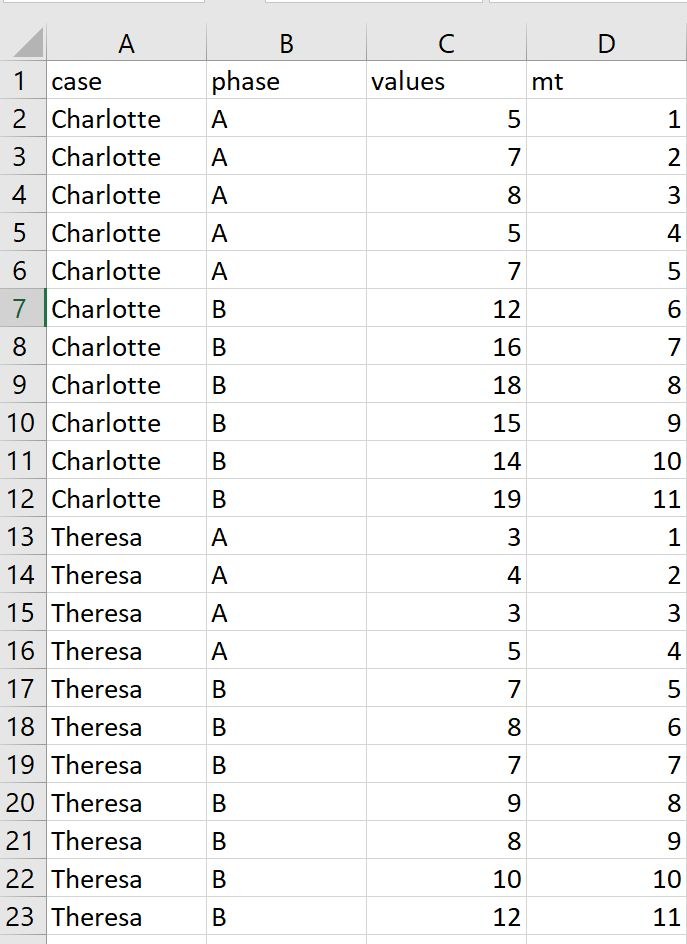
\includegraphics[width=3.125in,height=\textheight]{./images/readSC.jpg}

}

\caption{How to format a single-case file in a spreadsheet program for
importing into scan}

\end{figure}

In case your variables names differ from the standard (i.e.~``case'',
``values'', ``phase'', and ``mt'' ), you could set additional arguments
to fit your file.
\texttt{read\_scdf("example.csv",\ cvar\ =\ "name",\ dvar\ =\ "wellbeing",\ pvar\ =\ "intervention",\ mvar\ =\ "time")}
for example will set the variables attributes of the resulting scdf.
Cases will be split by the variable \texttt{"name"},
\texttt{"wellbeing"} is set as the dependent variable (default is
\emph{values}), phase information are in the variable
\texttt{"intervention"}, and measurement times in the variable
\texttt{"time"}. You could also reassign the phase names within the
phase variable by setting the argument \texttt{phase.names}. Assume for
example your file contains the values 0 and 1 to identify the two phases
I recommend to set them to ``A'' and ``B'' with
\texttt{read\_scdf("example.csv",\ phase.names\ =\ c("A",\ "B"))}.

\begin{Shaded}
\begin{Highlighting}[]
\NormalTok{dat }\OtherTok{\textless{}{-}} \FunctionTok{read\_scdf}\NormalTok{(}
  \StringTok{"example2.xlsx"}\NormalTok{, }\AttributeTok{cvar =} \StringTok{"name"}\NormalTok{, }\AttributeTok{pvar =} \StringTok{"intervention"}\NormalTok{, }
  \AttributeTok{dvar =} \StringTok{"wellbeing"}\NormalTok{, }\AttributeTok{mvar =} \StringTok{"time"}\NormalTok{, }\AttributeTok{phase.names =} \FunctionTok{c}\NormalTok{(}\StringTok{"A"}\NormalTok{,}\StringTok{"B"}\NormalTok{)}
\NormalTok{)}
\end{Highlighting}
\end{Shaded}

\begin{verbatim}
Loaded 20 cases.
\end{verbatim}

\begin{Shaded}
\begin{Highlighting}[]
\FunctionTok{summary}\NormalTok{(dat)}
\end{Highlighting}
\end{Shaded}

\begin{verbatim}
#A single-case data frame with 20 cases

          Measurements Design
 Charles            20    A-B
 Kolten             20    A-B
 Annika             20    A-B
 Kaysen             20    A-B
 Urijah             20    A-B
 Leila              20    A-B
 Leia               20    A-B
 Aleigha            20    A-B
 Greta              20    A-B
 Alijah             20    A-B
 Ricardo            20    A-B
 Dallas             20    A-B
 Edith              20    A-B
 Braylee            20    A-B
 Giovanni           20    A-B
 Ismael             20    A-B
 Grady              20    A-B
 Raina              20    A-B
 Cambria            20    A-B
 Lincoln            20    A-B

Variable names:
intervention <phase variable>
wellbeing <dependent variable>
time <measurement-time variable>
age
gender
gym
\end{verbatim}

For some reasons, computer systems with a German (and some other)
language setups export csv-files by default with a comma as a decimal
point and a semicolon as a separator between values. In these cases you
have to set two extra arguments to import the data:

\texttt{read\_scdf("example.csv",\ dec\ =\ ",",\ sep\ =\ ";")}

\texttt{read\_scdf} also allows for directly importing \emph{Microsoft
Excel} \texttt{.xlsx} or \texttt{.xls} files. You need to have the
library \texttt{readxl} installed in your R setup for this to work.
Excel files will be automatically detected by the filename extension
\texttt{xls}or \texttt{xlsx} or by explicitly setting the \texttt{type}
argument (e.g.~\texttt{type\ =\ "xlsx"}).

\hypertarget{sec-write-scdf}{%
\subsection{Export data}\label{sec-write-scdf}}

\begin{tcolorbox}[enhanced jigsaw, toprule=.15mm, colframe=quarto-callout-tip-color-frame, left=2mm, colback=white, breakable, bottomrule=.15mm, arc=.35mm, rightrule=.15mm, leftrule=.75mm, opacityback=0]
\begin{minipage}[t]{5.5mm}
\textcolor{quarto-callout-tip-color}{\faLightbulb}
\end{minipage}%
\begin{minipage}[t]{\textwidth - 5.5mm}
write\_scdf(data, filename = NULL, sep = ``,'', dec = ``.'',
\ldots)\end{minipage}%
\end{tcolorbox}

\texttt{write\_scdf()} exports an scdf object as a
comma-separated-variables file (\emph{csv}) which can be imported into
any other software for data analyses (MS OFFICE, Libre Office etc.). The
scdf object is converted into a single data frame with a \emph{case}
variable identifying the rows for each subject. The first argument of
the command identifies the scdf to be exported and the second argument
(\texttt{file}) the name of the resulting csv-file. If no file argument
is provided, a dialog box is opened to choose a file interactively. By
default, writeSC exports into a standard csv-format with a dot as the
decimal point and a comma for separating variables. If your system
expects a comma instead of a point for decimal numbers you may use the
\texttt{dec} and the \texttt{sep} arguments. For example,
\texttt{write\_scdf(example,\ file\ =\ "example.csv",\ dec\ =\ ",",\ sep\ =\ ";")}
exports a csv variation usually used for example in Germany.

\hypertarget{sec-convert}{%
\section{Convert an scdf object back to scan syntax}\label{sec-convert}}

\begin{tcolorbox}[enhanced jigsaw, toprule=.15mm, colframe=quarto-callout-tip-color-frame, left=2mm, colback=white, breakable, bottomrule=.15mm, arc=.35mm, rightrule=.15mm, leftrule=.75mm, opacityback=0]
\begin{minipage}[t]{5.5mm}
\textcolor{quarto-callout-tip-color}{\faLightbulb}
\end{minipage}%
\begin{minipage}[t]{\textwidth - 5.5mm}
convert(scdf, file = ````, study\_name =''study'')\end{minipage}%
\end{tcolorbox}

You can also reconvert an scdf object back to ``raw'' scan syntax. This
is a convenient way when you imported data from an Excel or csv file and
want to keep everything clean and transparent within your R syntax
files.

Here is an example:

\begin{Shaded}
\begin{Highlighting}[]
\FunctionTok{convert}\NormalTok{(exampleABC)}
\end{Highlighting}
\end{Shaded}

\begin{verbatim}
case1 <- scdf(
   values = c(58, 56, 60, 63, 51, 45, 44, 59, 45, 39, 83, 65, 70, 83, 70, 85, 47, 66, 77, 75, 51, 87, 80, 68, 70, 56, 52, 70, 83, 63), 
   phase_design = c(A = 10, B = 10, C = 10),
   name = "Marie"
)

case2 <- scdf(
   values = c(47, 41, 47, 52, 54, 65, 55, 37, 51, 60, 60, 65, 55, 46, 49, 54, 77, 73, 97, 64, 84, 71, 66, 74, 78, 68, 52, 76, 63, 54), 
   phase_design = c(A = 15, B = 8, C = 7),
   name = "Rosalind"
)

case3 <- scdf(
   values = c(50, 45, 63, 53, 66, 57, 35, 45, 74, 63, 47, 45, 47, 36, 51, 55, 35, 66, 59, 55, 73, 60, 85, 62, 79, 69, 87, 76, 90, 48), 
   phase_design = c(A = 20, B = 7, C = 3),
   name = "Lise"
)

study <- c(case1, case2, case3)
\end{verbatim}

Now you can copy and past the output into your R file or you set the
\texttt{file} argument to save the output into an R file
\texttt{convert(exampleABC,\ file\ =\ "scdf.R")}.

\hypertarget{displaying-scdf-files}{%
\section{Displaying scdf-files}\label{displaying-scdf-files}}

\emph{scdf} are displayed by just typing the name of the object.

\begin{Shaded}
\begin{Highlighting}[]
\CommentTok{\#Beretvas2008 is an example scdf included in scan}
\NormalTok{Beretvas2008}
\end{Highlighting}
\end{Shaded}

\begin{verbatim}
#A single-case data frame with one case

 Case1: values mt phase
           0.7  1     A
           1.6  2     A
           1.4  3     A
           1.6  4     A
           1.9  5     A
           1.2  6     A
           1.3  7     A
           1.6  8     A
            10  9     B
          10.8 10     B
          11.9 11     B
            11 12     B
            13 13     B
          12.7 14     B
            14 15     B
\end{verbatim}

The \texttt{print} command allows for specifying the output. Some
possible arguments are \texttt{cases} (the number of cases to be
displayed; Three by default), \texttt{rows} (the maximum number of rows
to be displayed; Fifteen by default), and \texttt{digits} (number of
digits). \texttt{cases\ =\ \textquotesingle{}all\textquotesingle{}} and
\texttt{rows\ =\ \textquotesingle{}all\textquotesingle{}} prints all
cases and rows.

\begin{Shaded}
\begin{Highlighting}[]
\CommentTok{\#Huber2014 is an example scdf included in scan}
\FunctionTok{print}\NormalTok{(Huber2014, }\AttributeTok{cases =} \DecValTok{2}\NormalTok{, }\AttributeTok{rows =} \DecValTok{10}\NormalTok{)}
\end{Highlighting}
\end{Shaded}

\begin{verbatim}
#A single-case data frame with 4 cases

 Adam: mt compliance phase | Berta: mt compliance phase |
        1         25     A |         1         25     A |
        2       20.8     A |         2       20.8     A |
        3       39.6     A |         3       39.6     A |
        4         75     A |         4         75     A |
        5         45     A |         5         45     A |
        6       39.6     A |         6       14.6     A |
        7       54.2     A |         7       45.8     A |
        8         50     A |         8       33.3     A |
        9       28.1     A |         9       31.3     A |
       10         40     A |        10       32.5     A |
# ... up to 66 more rows
#  2 more cases
\end{verbatim}

The argument \texttt{long\ =\ TRUE} prints each case one after the other
instead side by side (e.g., \texttt{print(exampleAB,\ long\ =\ TRUE)}).

\texttt{summary()} gives a very concise overview of the \emph{scdf}

\begin{Shaded}
\begin{Highlighting}[]
\FunctionTok{summary}\NormalTok{(Huber2014)}
\end{Highlighting}
\end{Shaded}

\begin{verbatim}
#A single-case data frame with 4 cases

           Measurements Design
 Adam                37    A-B
 Berta               29    A-B
 Christian           76    A-B
 David               76    A-B

Variable names:
mt <measurement-time variable>
compliance <dependent variable>
phase <phase variable>


Note:  Behavioral data (compliance in percent).
Author of data:  Christian Huber 
\end{verbatim}

\hypertarget{selecting-cases-and-measurements}{%
\section{Selecting cases and
measurements}\label{selecting-cases-and-measurements}}

\hypertarget{subsetting-cases-with-base-r-syntax}{%
\subsection{Subsetting cases with base R
syntax}\label{subsetting-cases-with-base-r-syntax}}

You can extract one or more single-cases from an \emph{scdf} with
multiple cases in two ways. If the case has a name, you can address it
with the \texttt{\$} operator.

\begin{Shaded}
\begin{Highlighting}[]
\NormalTok{Huber2014}\SpecialCharTok{$}\NormalTok{David}
\end{Highlighting}
\end{Shaded}

or you can use squared brackets

\begin{Shaded}
\begin{Highlighting}[]
\NormalTok{Huber2014[}\DecValTok{1}\NormalTok{] }\CommentTok{\#extracts case 1}
\NormalTok{Huber2014[}\DecValTok{2}\SpecialCharTok{:}\DecValTok{3}\NormalTok{] }\CommentTok{\#extracts cases 2 and 3}
\end{Highlighting}
\end{Shaded}

\begin{Shaded}
\begin{Highlighting}[]
\NormalTok{new.huber2014 }\OtherTok{\textless{}{-}}\NormalTok{ Huber2014[}\FunctionTok{c}\NormalTok{(}\DecValTok{1}\NormalTok{, }\DecValTok{4}\NormalTok{)] }\CommentTok{\#extracts cases 1 and 4}
\NormalTok{new.huber2014}
\end{Highlighting}
\end{Shaded}

\begin{verbatim}
#A single-case data frame with 2 cases

 Adam: mt compliance phase | David: mt compliance phase |
        1         25     A |         1       65.6     A |
        2       20.8     A |         2       37.5     A |
        3       39.6     A |         3       58.3     A |
        4         75     A |         4       72.9     A |
        5         45     A |         5       33.3     A |
        6       39.6     A |         6       59.4     A |
        7       54.2     A |         7       77.1     A |
        8         50     A |         8       54.2     A |
        9       28.1     A |         9       68.8     A |
       10         40     A |        10       43.8     A |
       11       52.1     B |        11       62.5     B |
       12       31.3     B |        12       64.6     B |
       13       15.6     B |        13       60.4     B |
       14       29.2     B |        14       81.3     B |
       15       43.8     B |        15       79.2     B |
# ... up to 61 more rows
\end{verbatim}

\hypertarget{sec-select-cases}{%
\subsection{Select cases}\label{sec-select-cases}}

\begin{tcolorbox}[enhanced jigsaw, toprule=.15mm, colframe=quarto-callout-tip-color-frame, left=2mm, colback=white, breakable, bottomrule=.15mm, arc=.35mm, rightrule=.15mm, leftrule=.75mm, opacityback=0]
\begin{minipage}[t]{5.5mm}
\textcolor{quarto-callout-tip-color}{\faLightbulb}
\end{minipage}%
\begin{minipage}[t]{\textwidth - 5.5mm}
select\_cases(scdf, \ldots)\end{minipage}%
\end{tcolorbox}

Since version 0.53 scan includes some functions to work with
pipe-operators. Therefore, we will provide syntax examples with and
without pipe operators.

The \texttt{select\_cases()} function takes case-names and/or numbers
for selecting cases:

\begin{Shaded}
\begin{Highlighting}[]
\CommentTok{\# With pipes:}
\NormalTok{Huber2014 }\SpecialCharTok{\%\textgreater{}\%}
  \FunctionTok{select\_cases}\NormalTok{(}\StringTok{"Adam"}\NormalTok{, }\StringTok{"Berta"}\NormalTok{, }\DecValTok{4}\NormalTok{) }\SpecialCharTok{\%\textgreater{}\%}
  \FunctionTok{summary}\NormalTok{()}
\end{Highlighting}
\end{Shaded}

\begin{verbatim}
#A single-case data frame with 3 cases

       Measurements Design
 Adam            37    A-B
 Berta           29    A-B
 David           76    A-B

Variable names:
mt <measurement-time variable>
compliance <dependent variable>
phase <phase variable>


Note:  Behavioral data (compliance in percent).
Author of data:  Christian Huber 
\end{verbatim}

\begin{Shaded}
\begin{Highlighting}[]
\CommentTok{\# Without pipes:}

\CommentTok{\# new\_huber \textless{}{-} select\_cases(Huber2014, "Adam", "Berta", 4)}
\CommentTok{\# summary(new\_huber)}
\end{Highlighting}
\end{Shaded}

\hypertarget{sec-subset}{%
\subsection{Select measurements}\label{sec-subset}}

The \texttt{subset()} function helps with extracting measurements (or
rows) by a specific criteria from a scdf.

Subset takes a scdf as its first argument and a logical expression as
the second argument (\texttt{filter}). Only measurements for which the
logical argument is evaluated to be TRUE are inlcuded in the returning
scdf object.

For example, the scdf \texttt{Huber2014} has a variable
\texttt{compliance} and we like to keep measurements where
\texttt{compliance} is larger than 10 because we assume the others to be
outliers:

\begin{Shaded}
\begin{Highlighting}[]
\NormalTok{Huber2014 }\SpecialCharTok{\%\textgreater{}\%}
  \FunctionTok{subset}\NormalTok{(compliance }\SpecialCharTok{\textgreater{}} \DecValTok{10}\NormalTok{) }\SpecialCharTok{\%\textgreater{}\%}
  \FunctionTok{summary}\NormalTok{()}
\end{Highlighting}
\end{Shaded}

\begin{verbatim}
#A single-case data frame with 4 cases

           Measurements Design
 Adam                37    A-B
 Berta               20    A-B
 Christian           76    A-B
 David               76    A-B

Variable names:
mt <measurement-time variable>
compliance <dependent variable>
phase <phase variable>


Note:  Behavioral data (compliance in percent).
Author of data:  Christian Huber 
\end{verbatim}

In an more complex example, we only like to keep values lower than 60
when they are in phase A or values equal or larger than 60 when they are
in phase B:

\begin{Shaded}
\begin{Highlighting}[]
\NormalTok{exampleAB }\SpecialCharTok{\%\textgreater{}\%}
  \FunctionTok{subset}\NormalTok{((values }\SpecialCharTok{\textless{}} \DecValTok{60} \SpecialCharTok{\&}\NormalTok{ phase }\SpecialCharTok{==} \StringTok{"A"}\NormalTok{) }\SpecialCharTok{|}\NormalTok{ (values }\SpecialCharTok{\textgreater{}=} \DecValTok{60} \SpecialCharTok{\&}\NormalTok{ phase }\SpecialCharTok{==} \StringTok{"B"}\NormalTok{)) }\SpecialCharTok{\%\textgreater{}\%}
  \FunctionTok{summary}\NormalTok{()}
\end{Highlighting}
\end{Shaded}

\begin{verbatim}
#A single-case data frame with 3 cases

          Measurements Design
 Johanna            20    A-B
 Karolina           18    A-B
 Anja               19    A-B

Variable names:
values <dependent variable>
mt <measurement-time variable>
phase <phase variable>


Note:  Randomly created data with normal distributed dependent variable.
\end{verbatim}

\hypertarget{change-and-create-variables}{%
\section{Change and create
variables}\label{change-and-create-variables}}

\hypertarget{creating-a-single-case-data-plot}{%
\chapter{Creating a single-case data
plot}\label{creating-a-single-case-data-plot}}

\begin{tcolorbox}[enhanced jigsaw, toprule=.15mm, colframe=quarto-callout-tip-color-frame, left=2mm, colback=white, breakable, bottomrule=.15mm, arc=.35mm, rightrule=.15mm, leftrule=.75mm, opacityback=0]
\begin{minipage}[t]{5.5mm}
\textcolor{quarto-callout-tip-color}{\faLightbulb}
\end{minipage}%
\begin{minipage}[t]{\textwidth - 5.5mm}
plotSC(data, dvar, pvar, mvar, ylim = NULL, xlim = NULL, xinc = 1, lines
= NULL, marks = NULL, phase.names = NULL, xlab = NULL, ylab = NULL, main
= ````, case.names = NULL, style = getOption(''scan.plot.style''),
\ldots)\end{minipage}%
\end{tcolorbox}

Plotting the data is a first important approach of analyzing. After you
build an \emph{scdf} the \texttt{plot} command helps to visualize the
data. When the \texttt{scdf} includes more than one case a multiple
baseline figure is provided. Various arguments can be set to customize
the appearance of the plot. Table~\ref{tbl-plot-arguments} gives an
overview of all available arguments.

\begin{Shaded}
\begin{Highlighting}[]
\FunctionTok{plot}\NormalTok{(exampleA1B1A2B2\_zvt)}
\end{Highlighting}
\end{Shaded}

\begin{figure}[H]

{\centering 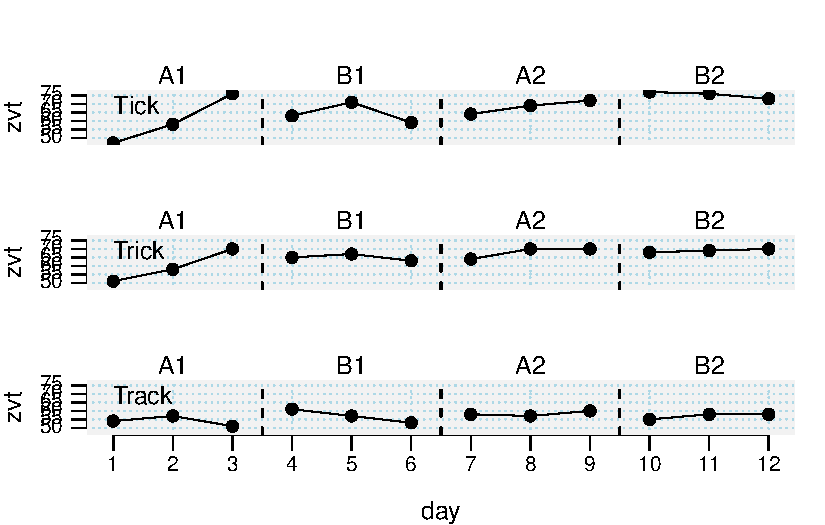
\includegraphics{./ch_creating_a_plot_files/figure-pdf/ex-simple-plot-1.pdf}

}

\caption{A simple plot does not need much.}

\end{figure}

\hypertarget{plot-axis}{%
\section{Plot axis}\label{plot-axis}}

Labels of the axes and for the phases can be changed with the
\texttt{xlab}, \texttt{ylab}, and the \texttt{phase.names} arguments.
The x- and y-scaling of the graphs are by default calculated as the
minimum and the maximum of all included single cases. The \texttt{xlim}
and the \texttt{ylim} argument are used to set specific values. The
argument takes a vector of two numbers. The first for the lower and the
second for the upper limit of the scale. In case of multiple single
cases an \texttt{NA} sets the individual minimum or maximum for each
case. Assume for example the study contains three single cases
\texttt{ylim\ =\ c(0,\ NA)} will set the lower limit for all three
single cases to \texttt{0} and the upper limit individually at the
maximum of each case. The argument \texttt{xinc} sets the incremental
steps for the x-axis ticks with corresponding values. For example
\texttt{xinc\ =\ 1} will set a tick for every measurement time increase
of 1 while \texttt{xinc\ =\ 5} will only set every ffith tick.

\begin{Shaded}
\begin{Highlighting}[]
\FunctionTok{plot}\NormalTok{(}
\NormalTok{  exampleABC,}
  \AttributeTok{phase.names =} \FunctionTok{c}\NormalTok{(}\StringTok{"Baseline"}\NormalTok{, }\StringTok{"Intervention"}\NormalTok{, }\StringTok{"Follow{-}Up"}\NormalTok{),}
  \AttributeTok{case.names =} \FunctionTok{c}\NormalTok{(}\StringTok{"First"}\NormalTok{, }\StringTok{"Second"}\NormalTok{, }\StringTok{"Third"}\NormalTok{),}
  \AttributeTok{ylab =} \StringTok{"Frequency"}\NormalTok{,}
  \AttributeTok{xlab =} \StringTok{"Days"}\NormalTok{,}
  \AttributeTok{main =} \StringTok{"An example"}\NormalTok{,}
  \AttributeTok{ylim =} \FunctionTok{c}\NormalTok{(}\DecValTok{0}\NormalTok{, }\DecValTok{120}\NormalTok{),}
  \AttributeTok{xinc =} \DecValTok{2}
\NormalTok{)}
\end{Highlighting}
\end{Shaded}

\begin{figure}[H]

{\centering 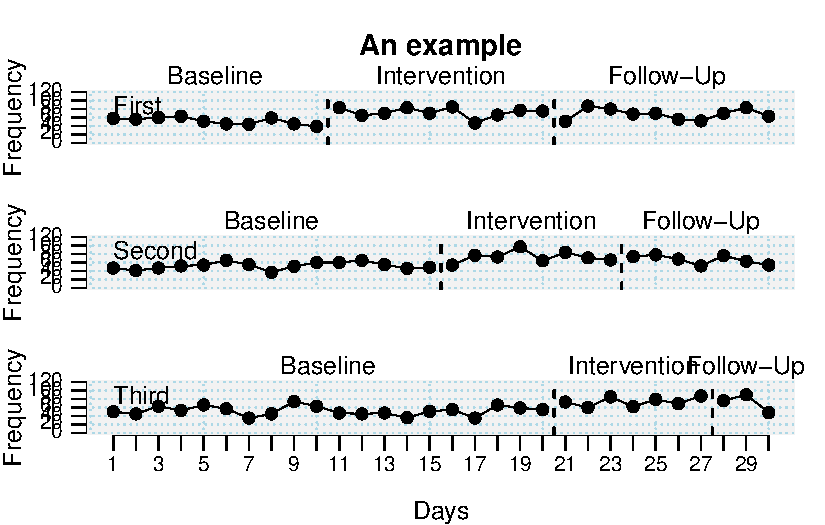
\includegraphics{./ch_creating_a_plot_files/figure-pdf/ex-plot-axis-1.pdf}

}

\caption{A plot with various axis specidications.}

\end{figure}

\hypertarget{tbl-plot-arguments}{}
\begin{longtable}[]{@{}ll@{}}
\caption{\label{tbl-plot-arguments}Arguments of the plot
function}\tabularnewline
\toprule()
Argument & What it does ... \\
\midrule()
\endfirsthead
\toprule()
Argument & What it does ... \\
\midrule()
\endhead
data & A single-case data frame. \\
ylim & Lower and upper limits of the y-axis \\
xlim & Lower and upper limits of the x-axis. \\
style & A specific design for displaying the plot. \\
lines & A character or list defining one or more lines or curves to be
plotted. \\
marks & A list of parameters defining markings of certain data
points. \\
main & A figure title \\
phase.names & By default phases are labeled as given in the phase
variable. Use this argument to specify different labels: `phase.names =
c(\textquotesingle Baseline\textquotesingle,
\textquotesingle Intervention\textquotesingle)`. \\
case.names & Case names. If not provided, names are taken from the scdf
or left blank if the scdf does not contain case names. \\
xlab & The label of the x-axis. The default is taken from the name of
the measurement variable as provided by the scdf. \\
ylab & The labels of the y-axis. The default is taken from the name of
the dependent variable as provided by the scdf. \\
xinc & An integer. Increment of the x-axis. 1 : each mt value will be
printed, 2 : every other value, 3 : every third values etc. \\
\bottomrule()
\end{longtable}

\hypertarget{adding-lines}{%
\section{Adding lines}\label{adding-lines}}

Extra lines can be added to the plot using the \texttt{lines} argument.
The lines argument takes several separate sub-arguments which have to be
provided in a list. In its most simple form this list contains one
element.
\texttt{lines\ =\ list(type\ =\ \textquotesingle{}median\textquotesingle{})}
adds a line with the median of each phase to the plot. Additional
arguments like \texttt{col} or \texttt{lwd} help to format these lines.
For adding red thick median lines use the command
\texttt{lines\ =\ list(type\ =\ \textquotesingle{}median\textquotesingle{},\ col\ =\ \textquotesingle{}red\textquotesingle{},\ lwd\ =\ \textquotesingle{}2\textquotesingle{})}.

\hypertarget{tbl-lines-arguments}{}
\begin{longtable}[]{@{}ll@{}}
\caption{\label{tbl-lines-arguments}Values of the lines
argument}\tabularnewline
\toprule()
Argument & What it does ... \\
\midrule()
\endfirsthead
\toprule()
Argument & What it does ... \\
\midrule()
\endhead
median & separate lines for the medians of each phase \\
mean & separate lines for the means of each phase. By default it is
10\%-trimmed. Other trims can be set using a second parameter (e.g.,
`lines = list(type = \textquotesingle mean\textquotesingle, trim = 0.2)`
draws a 20\%-trimmed mean line). \\
trend & Separate lines for the trend of each phase. \\
trendA & Trend line for phase A, extrapolated throughout the other
phases \\
maxA & Line at the level of the highest phase A score. \\
minA & Line at the level of the lowest phase A score. \\
medianA & Line at the phase A median score. \\
meanA & Line at the phase A 10\%-trimmed mean score. Apply a different
trim, by using the additional argument (e.g., `lines = list(type =
\textquotesingle meanA\textquotesingle, trim = 0.2)`). \\
movingMean & Draws a moving mean curve, with a specified lag: `lines =
list(type = \textquotesingle movingMean\textquotesingle, lag = 2)`.
Default is a lag 1 curve. \\
movingMedian & Draws a moving median curve, with a specified lag: `lines
= list(type = \textquotesingle movingMedian\textquotesingle, lag = 3).`
Default is a lag 1 curve. \\
loreg & Draws a non-parametric local regression line. The proportion of
data influencing each data point can be specified using `lines =
list(type = \textquotesingle loreg\textquotesingle, f = 0.66)`. The
default is 0.5. \\
lty & Line type. Examples are:
\textquotesingle solid\textquotesingle,\textquotesingle dashed\textquotesingle,
\textquotesingle dotted\textquotesingle. \\
lwd & Line thickness, e.g., `lwd = 4`. \\
col & Line colour, e.g., `col =
\textquotesingle red\textquotesingle`. \\
\bottomrule()
\end{longtable}

\begin{Shaded}
\begin{Highlighting}[]
\FunctionTok{plot}\NormalTok{(}
\NormalTok{  exampleAB, }
  \AttributeTok{lines =} \FunctionTok{list}\NormalTok{(}
    \FunctionTok{list}\NormalTok{(}\AttributeTok{type =} \StringTok{"median"}\NormalTok{, }\AttributeTok{col =} \StringTok{"red"}\NormalTok{, }\AttributeTok{lwd =} \FloatTok{0.5}\NormalTok{),}
    \FunctionTok{list}\NormalTok{(}\AttributeTok{type =} \StringTok{"trend"}\NormalTok{, }\AttributeTok{col =} \StringTok{"blue"}\NormalTok{, }\AttributeTok{lty =} \StringTok{"dashed"}\NormalTok{, }\AttributeTok{lwd =} \DecValTok{2}\NormalTok{),}
    \FunctionTok{list}\NormalTok{(}\AttributeTok{type =} \StringTok{"loreg"}\NormalTok{, }\AttributeTok{f =} \FloatTok{0.2}\NormalTok{, }\AttributeTok{col =} \StringTok{"green"}\NormalTok{, }\AttributeTok{lty =} \StringTok{"solid"}\NormalTok{, }\AttributeTok{lwd =} \DecValTok{1}\NormalTok{)}
\NormalTok{  )}
\NormalTok{)}
\end{Highlighting}
\end{Shaded}

\begin{figure}[H]

{\centering 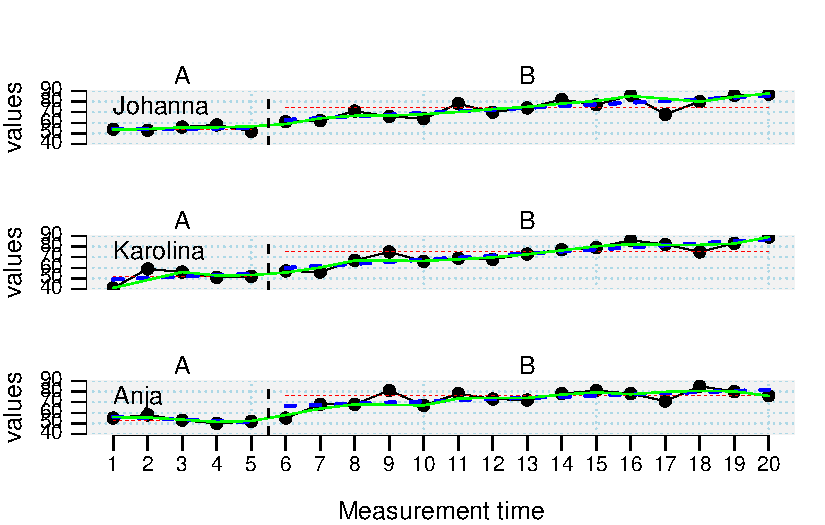
\includegraphics{./ch_creating_a_plot_files/figure-pdf/ex-plot-lines-1.pdf}

}

\caption{A plot with various visual aids}

\end{figure}

\hypertarget{mark-data-points}{%
\section{Mark data points}\label{mark-data-points}}

Specific data points can be highlighted using the \texttt{marks}
argument. A \texttt{list} defines the measurement times to be marked,
the marking color and the size of the marking.
\texttt{marks\ =\ list(position\ =\ c(1,5,6))} marks the first, fifth,
and sixth measurement time. If the \emph{scdf} contains more than one
data-set marking would be the same for all data sets in this example. In
case you define a \texttt{list} Containing vectors, marking can be
individually defined for each data set. Assume, for example, we have an
\emph{scdf} comprising three data sets, then
\texttt{marks\ =\ list(position\ =\ list(c(1,2),\ c(3,4),\ c(5,6)))}
will highlight measurement times one and two for the first data set,
three and four for the second and five and six for the third.
\texttt{pch}, \texttt{col} and \texttt{cex} define symbol, colour and
size of the markings.

\begin{Shaded}
\begin{Highlighting}[]
\CommentTok{\# plot with marks in a red circles 2.5 times larger than the standard symbol }
\CommentTok{\# size. exampleAB is an example scdf included in the scan package}
\NormalTok{marks }\OtherTok{\textless{}{-}} \FunctionTok{list}\NormalTok{(}
  \AttributeTok{positions =} \FunctionTok{list}\NormalTok{( }\FunctionTok{c}\NormalTok{(}\DecValTok{8}\NormalTok{, }\DecValTok{9}\NormalTok{), }\FunctionTok{c}\NormalTok{(}\DecValTok{17}\NormalTok{, }\DecValTok{19}\NormalTok{), }\FunctionTok{c}\NormalTok{(}\DecValTok{7}\NormalTok{, }\DecValTok{18}\NormalTok{) ), }
  \AttributeTok{col =} \StringTok{\textquotesingle{}red\textquotesingle{}}\NormalTok{, }\AttributeTok{cex =} \FloatTok{2.5}\NormalTok{, }\AttributeTok{pch =} \DecValTok{1}
\NormalTok{)}
\FunctionTok{plot}\NormalTok{(exampleAB, }\AttributeTok{marks =}\NormalTok{ marks, }\AttributeTok{style =} \StringTok{"sienna"}\NormalTok{)}
\end{Highlighting}
\end{Shaded}

\begin{figure}[H]

{\centering 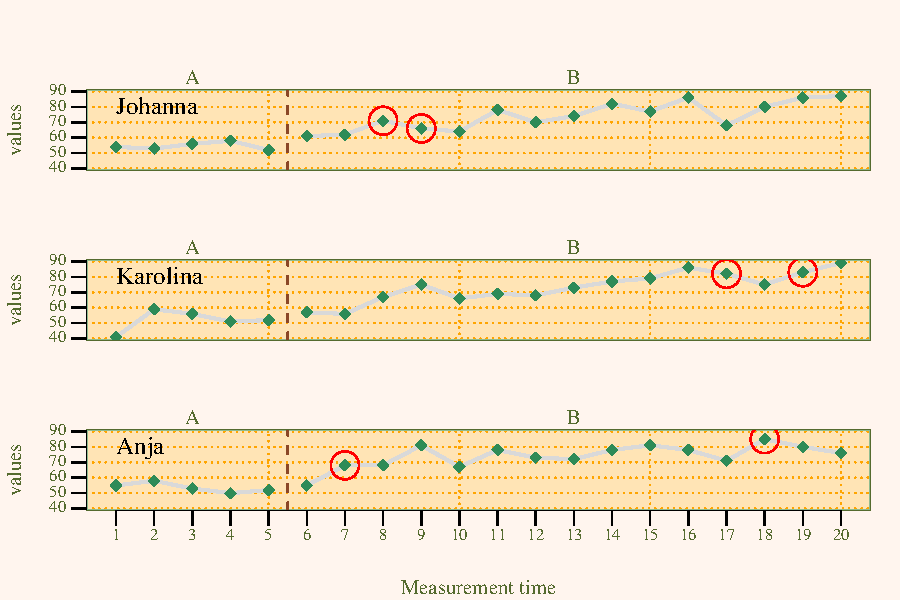
\includegraphics{./ch_creating_a_plot_files/figure-pdf/marks-example-1.pdf}

}

\caption{A plot with highlighted data-points}

\end{figure}

\hypertarget{graphical-styles-of-a-plot}{%
\section{Graphical styles of a plot}\label{graphical-styles-of-a-plot}}

\begin{tcolorbox}[enhanced jigsaw, toprule=.15mm, colframe=quarto-callout-tip-color-frame, left=2mm, colback=white, breakable, bottomrule=.15mm, arc=.35mm, rightrule=.15mm, leftrule=.75mm, opacityback=0]
\begin{minipage}[t]{5.5mm}
\textcolor{quarto-callout-tip-color}{\faLightbulb}
\end{minipage}%
\begin{minipage}[t]{\textwidth - 5.5mm}
style\_plot(style = ``default'', \ldots)\end{minipage}%
\end{tcolorbox}

The \texttt{style} argument of the plot function allows to specify a
specific design of a plot. By default, the \texttt{grid} style is
applied. \texttt{scan} includes some further predefined styles.
\texttt{default,\ yaxis,\ tiny,\ small,\ big,\ chart,\ ridge,\ annotate,\ grid,\ grid2,\ dark,\ nodot,\ and\ sienna}.
The name of a style is provided as a character string (e.g.,
\texttt{style\ =\ "grid"}).\\
Some styles only address specific elements (e.g., ``small'' or ``tiny''
just influence text and line sizes). These styles lend themselves to be
combined with other styles. This could be achieved by providing several
style names to the plot argument:
\texttt{style\ =\ c("grid",\ "annotate",\ "small")}. A style overwrites
the settings of all previously included style.\\
Beyond predefined styles, styles can be individually modified and
created. New styles are provided as a \texttt{list} of several design
parameters that are passed to the \texttt{style} argument of the
\texttt{plot} function. Table~\ref{tbl-style} shows all design parameter
that could be defined.\\
To define a new style, first create a list containing a plain design.
The \texttt{style\_plot} function returns such a list with the default
values for a plain design (e.g.,
\texttt{mystyle\ \textless{}-\ style\_plot()}). Single design parameters
can now be set by assigning a specific value within the list. For
example, \texttt{newstyle\$fill\ \textless{}-\ "grey90"} will set the
\texttt{fill} parameter to \texttt{"grey90"}. Alternatively, changes to
the plain design can already by defined within the \texttt{style\_plot}
function. To set a light-blue background color and also an orange grid,
create the style
\texttt{style\_plot(fill.bg\ =\ "lightblue",\ grid\ =\ "orange")}. If
you do not want to start with the plain design but a different of the
predefined styles, set the \texttt{style} argument. If, for example, you
like to have the \texttt{grid} combined with the \texttt{big} style but
want to change the color of the grid to orange type
\texttt{style\_plot(style\ =\ c("grid",\ "big"),\ col.grid\ =\ "orange")}.
\texttt{plot(mydata,\ style\ =\ mystyle)} will apply the new style in a
plot. Please note that the new style is not passed in quotation marks.

\hypertarget{tbl-style}{}
\begin{longtable}[]{@{}ll@{}}
\caption{\label{tbl-style}Arguments of the style plot
function}\tabularnewline
\toprule()
Argument & What it does ... \\
\midrule()
\endfirsthead
\toprule()
Argument & What it does ... \\
\midrule()
\endhead
fill & If TRUE area under the line is filled. \\
col.fill & Sets the color of the area under the line. \\
grid & If TRUE a grid is included. \\
col.grid & Sets the color of the grid. \\
lty.grid & Sets the line type of the grid. \\
lwd.grid & Sets the line thikness of the grid. \\
fill.bg & If not NA the backgorund of the plot is filled with the given
color. If multiple colours are provided, the colours change with phases
(e.g., `fill.bg = c(\textquotesingle aliceblue\textquotesingle,
\textquotesingle mistyrose1\textquotesingle,
\textquotesingle honeydew\textquotesingle)` \\
annotations & A list of parameters defining annotations to each data
point. This adds the score of each MT to your plot.
`\textquotesingle pos\textquotesingle` Position of the annotations: 1 =
below, 2 = left, 3 = above, 4 = right.
`\textquotesingle col\textquotesingle` Color of the annotations.
`\textquotesingle cex\textquotesingle` Size of the annotations.
`\textquotesingle round\textquotesingle` rounds the values to the
specified decimal. `annotations = list(pos = 3, col =
\textquotesingle brown\textquotesingle, round = 1)` adds scores rounded
to one decimal above the data point in brown color to the plot. \\
text.ABlag & By default a vertical line separates phases A and B in the
plot. Alternatively, you could print a character string between the two
phases using this argument: `text.ABlag =
\textquotesingle Start\textquotesingle`. \\
lwd & Width of the plot line. Default is `lwd = 2`. \\
pch & Point type. Default is `pch = 17` (triangles). Other options are
for example: 16 (filled circles) or \textquotesingle A\textquotesingle{}
(uses the letter A). \\
col.lines & The color of the lines. If set to an empty string no lines
are drawn. \\
col.dots & The color of the dots. If set to an empty string no dots are
drawn. \\
mai & Sets the margins of the plot. \\
... & Further arguments passed to the plot command. \\
\bottomrule()
\end{longtable}

The width of the lines are set with the \texttt{lwd} argument,
\texttt{col} is used to set the line colour and \texttt{pch} sets the
symbol for a data point. The \texttt{pch} argument can take several
values for defining the symbol in which data points are plotted.

\begin{figure}

{\centering 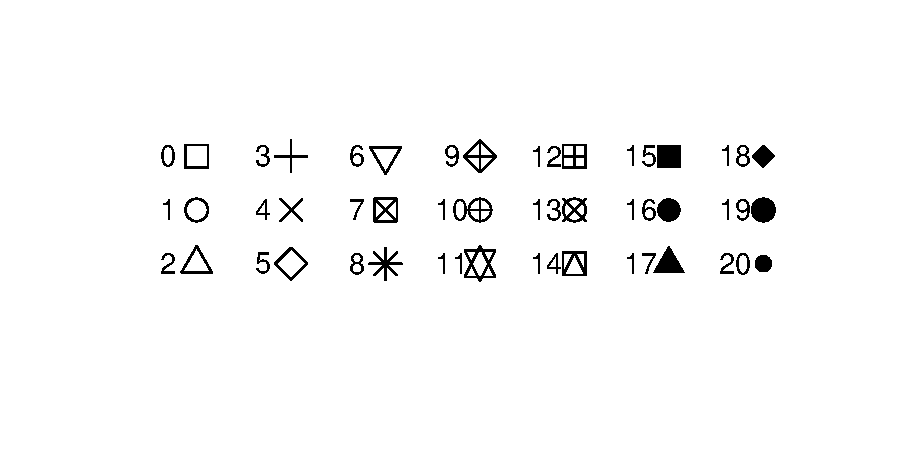
\includegraphics{./ch_creating_a_plot_files/figure-pdf/symbols, pch-1.pdf}

}

\caption{Some of the possible symbols and their pch values.}

\end{figure}

Here is an example customizing a plot with several additional graphic
parameters

\begin{Shaded}
\begin{Highlighting}[]
\NormalTok{newstyle }\OtherTok{\textless{}{-}} \FunctionTok{style\_plot}\NormalTok{(}
  \AttributeTok{fill =} \StringTok{"grey95"}\NormalTok{,}
  \AttributeTok{fill.bg =} \FunctionTok{c}\NormalTok{(}\StringTok{\textquotesingle{}aliceblue\textquotesingle{}}\NormalTok{, }\StringTok{\textquotesingle{}mistyrose1\textquotesingle{}}\NormalTok{, }\StringTok{\textquotesingle{}honeydew\textquotesingle{}}\NormalTok{),}
  \AttributeTok{names =} \FunctionTok{list}\NormalTok{(}\AttributeTok{col =} \StringTok{"brown"}\NormalTok{, }\AttributeTok{cex =} \DecValTok{2}\NormalTok{, }\AttributeTok{font =} \DecValTok{3}\NormalTok{, }\AttributeTok{side =} \DecValTok{3}\NormalTok{),}
  \AttributeTok{annotations =} \FunctionTok{list}\NormalTok{(}\AttributeTok{col =} \StringTok{"brown"}\NormalTok{),}
  \AttributeTok{col.dots =} \StringTok{"blue"}\NormalTok{,}
  \AttributeTok{grid =} \StringTok{"lightblue"}\NormalTok{, }
  \AttributeTok{pch =} \DecValTok{16}\NormalTok{)}

\FunctionTok{plot}\NormalTok{(exampleABAB, }\AttributeTok{style =}\NormalTok{ newstyle)}
\end{Highlighting}
\end{Shaded}

\begin{figure}[H]

{\centering 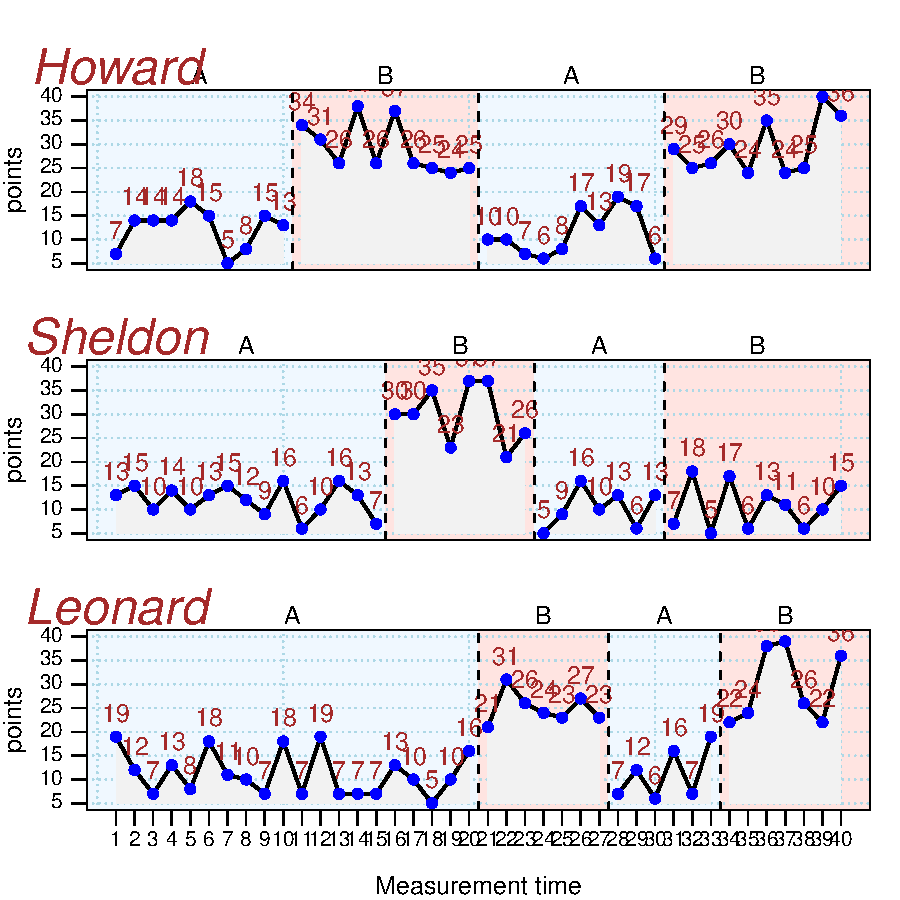
\includegraphics{./ch_creating_a_plot_files/figure-pdf/custom_style_example-1.pdf}

}

\caption{A plot with a customized style.}

\end{figure}

\hypertarget{describe-and-manipulate-single-case-data-frames}{%
\chapter{Describe and manipulate single-case data
frames}\label{describe-and-manipulate-single-case-data-frames}}

\hypertarget{describing-and-summarizing}{%
\section{Describing and summarizing}\label{describing-and-summarizing}}

A short description of the \emph{scdf} is provided by the
\texttt{summary} command. The results are pretty much self explaining

\begin{Shaded}
\begin{Highlighting}[]
\FunctionTok{summary}\NormalTok{(Huber2014)}
\end{Highlighting}
\end{Shaded}

\begin{verbatim}
#A single-case data frame with 4 cases

           Measurements Design
 Adam                37    A-B
 Berta               29    A-B
 Christian           76    A-B
 David               76    A-B

Variable names:
mt <measurement-time variable>
compliance <dependent variable>
phase <phase variable>


Note:  Behavioral data (compliance in percent).
Author of data:  Christian Huber 
\end{verbatim}

\begin{tcolorbox}[enhanced jigsaw, toprule=.15mm, colframe=quarto-callout-tip-color-frame, left=2mm, colback=white, breakable, bottomrule=.15mm, arc=.35mm, rightrule=.15mm, leftrule=.75mm, opacityback=0]
\begin{minipage}[t]{5.5mm}
\textcolor{quarto-callout-tip-color}{\faLightbulb}
\end{minipage}%
\begin{minipage}[t]{\textwidth - 5.5mm}
describe(data, dvar, pvar, mvar)\end{minipage}%
\end{tcolorbox}

\texttt{describe} is the basic command to get an overview on descriptive
statistics. As an argument it only takes the name of the \emph{scdf}
object. For each case of the \emph{scdf} and each phase within a case
descriptive statistics are provided. The output table contains
statistical indicators followed by a dot and the name of the phase
(e.g., \texttt{n.A} for the number of measurements of phase A).

\begin{longtable}[]{@{}ll@{}}
\caption{Statistics of the describe command }\tabularnewline
\toprule()
Parameter & What it means ... \\
\midrule()
\endfirsthead
\toprule()
Parameter & What it means ... \\
\midrule()
\endhead
n & Number of measurements. \\
mis & Number of missing values. \\
m & Mean values. \\
md & Median of values. \\
sd & Standard deviation of values. \\
mad & Median average deviation of values. \\
min/max & Min and max of values. \\
trend & Slope of a regression line through values by time. \\
\bottomrule()
\end{longtable}

\begin{Shaded}
\begin{Highlighting}[]
\FunctionTok{describe}\NormalTok{(exampleABC)}
\end{Highlighting}
\end{Shaded}

\begin{verbatim}
Describe Single-Case Data

       Marie Rosalind  Lise
Design A-B-C    A-B-C A-B-C
n.A       10       15    20
n.B       10        8     7
n.C       10        7     3
mis.A      0        0     0
mis.B      0        0     0
mis.C      0        0     0

          Marie Rosalind    Lise
m.A      52.000   52.267  52.350
m.B      72.100   73.250  73.571
m.C      68.000   66.429  71.333
md.A       53.5     52.0    52.0
md.B       72.5     72.0    73.0
md.C         69       68      76
sd.A      8.287    8.146  10.869
sd.B     11.367   13.134  10.644
sd.C     12.702   10.486  21.385
mad.A    11.119    7.413  10.378
mad.B    10.378   10.378  16.309
mad.C    17.791   11.861  20.756
min.A        39       37      35
min.B        47       54      60
min.C        51       52      48
max.A        63       65      74
max.B        85       97      87
max.C        87       78      90
trend.A  -1.915    0.500  -0.088
trend.B  -0.612    0.643   1.929
trend.C  -0.194   -2.929 -14.000
\end{verbatim}

The resulting table could be exported into a csv file to be used in
other software (e.g., to inserted in a word processing document).
Therefore, first write the results of the \texttt{describe} command into
an R object and then use the \texttt{write.csv} (or \texttt{write.csv2}
for a German OS system setup) to export the \texttt{descriptives}
element of the object.

\begin{Shaded}
\begin{Highlighting}[]
\CommentTok{\# write the results into a new R object named \textasciigrave{}res\textasciigrave{}}
\NormalTok{res }\OtherTok{\textless{}{-}} \FunctionTok{describe}\NormalTok{(exampleABC)}
\CommentTok{\# create a new file containing the descriptives on your harddrive}
\FunctionTok{write.csv}\NormalTok{(res}\SpecialCharTok{$}\NormalTok{descriptives, }\AttributeTok{file =} \StringTok{"descriptive data.csv"}\NormalTok{)}
\end{Highlighting}
\end{Shaded}

The file is written to the currently active working directory. If you
are not sure where that is, type \texttt{getwd()} (you can use the
\texttt{setwd()} command to define a different working directory. To get
further details type \texttt{help(setwd)} into R).

\begin{tcolorbox}[enhanced jigsaw, opacitybacktitle=0.6, breakable, bottomrule=.15mm, coltitle=black, colbacktitle=quarto-callout-note-color!10!white, colframe=quarto-callout-note-color-frame, left=2mm, colback=white, titlerule=0mm, leftrule=.75mm, opacityback=0, toptitle=1mm, title=\textcolor{quarto-callout-note-color}{\faInfo}\hspace{0.5em}{Conflicting function names}, arc=.35mm, rightrule=.15mm, toprule=.15mm, bottomtitle=1mm]

Sometimes R packages include the same function names. For example, the
\texttt{describe()} function is also part of the \texttt{psych} package.
Now, if you have loaded the \texttt{psych} package with
\texttt{library(psych)} after \texttt{scan} the \texttt{describe()}
function of scan will be masked (\texttt{describe()} would now call the
corresponding function of the \texttt{psych} package).\\
There are two solutions to this problem:

\begin{enumerate}
\def\labelenumi{\arabic{enumi}.}
\tightlist
\item
  activate the \texttt{psych} library before the \texttt{scan} library
  (now the psych \texttt{describe()} function will be masked) or
\item
  include the package name into the function call with the prefix
  \texttt{scan::}: \texttt{scan::describe()}.
\end{enumerate}

\end{tcolorbox}

\hypertarget{autoregression-and-trendanalyses}{%
\section{Autoregression and
trendanalyses}\label{autoregression-and-trendanalyses}}

\begin{tcolorbox}[enhanced jigsaw, toprule=.15mm, colframe=quarto-callout-tip-color-frame, left=2mm, colback=white, breakable, bottomrule=.15mm, arc=.35mm, rightrule=.15mm, leftrule=.75mm, opacityback=0]
\begin{minipage}[t]{5.5mm}
\textcolor{quarto-callout-tip-color}{\faLightbulb}
\end{minipage}%
\begin{minipage}[t]{\textwidth - 5.5mm}
autocorr(data, dvar, pvar, mvar, lag\_max = 3, \ldots)\end{minipage}%
\end{tcolorbox}

The \texttt{autocorr} function calculates autocorrelations within each
phase and across all phases. The \texttt{lag.max} argument defines the
lag up to which the autocorrelation will be computed.

\begin{Shaded}
\begin{Highlighting}[]
\FunctionTok{autocorr}\NormalTok{(exampleABC, }\AttributeTok{lag.max =} \DecValTok{4}\NormalTok{)}
\end{Highlighting}
\end{Shaded}

\begin{verbatim}
Autocorrelations

Marie 
 Phase Lag 1 Lag 2 Lag 3 Lag 4
     A  0.29 -0.11  0.10  0.12
     B -0.28 -0.10 -0.14 -0.09
     C  0.00 -0.33 -0.14 -0.25
   all  0.21  0.10  0.25  0.12

Rosalind 
 Phase Lag 1 Lag 2 Lag 3 Lag 4
     A  0.37 -0.29 -0.33 -0.34
     B -0.34  0.24 -0.40  0.04
     C -0.07 -0.32  0.27  0.02
   all  0.49  0.38  0.22  0.17

Lise 
 Phase Lag 1 Lag 2 Lag 3 Lag 4
     A  0.04 -0.32 -0.05 -0.09
     B -0.63  0.50 -0.40  0.31
     C -0.38 -0.12    NA    NA
   all  0.33  0.36  0.23  0.27
\end{verbatim}

The \texttt{trend} function provides an overview of linear trends in
single-case data. By default, it gives you the intercept and slope of a
linear and a squared regression of measurement-time on scores. Models
are computed separately for each phase and across all phases. For a more
advanced application, you can add regression models using the R specific
formula class.

\begin{Shaded}
\begin{Highlighting}[]
\CommentTok{\# Simple example}
\FunctionTok{trend}\NormalTok{(exampleABC[}\DecValTok{1}\NormalTok{])}
\end{Highlighting}
\end{Shaded}

\begin{verbatim}
Trend for each phase

            Intercept      B   Beta
Linear.ALL     55.159  0.612  0.392
Linear.A       60.618 -1.915 -0.700
Linear.B       74.855 -0.612 -0.163
Linear.C       68.873 -0.194 -0.046
Squared.ALL    59.135  0.017  0.330
Squared.A      57.937 -0.208 -0.712
Squared.B      73.217 -0.039 -0.098
Squared.C      68.490 -0.017 -0.038

Note. Measurement-times start at 0  for each phase
\end{verbatim}

\begin{Shaded}
\begin{Highlighting}[]
\CommentTok{\# Complex example}
\FunctionTok{trend}\NormalTok{(exampleAB}\SpecialCharTok{$}\NormalTok{Johanna, }\AttributeTok{offset =} \DecValTok{0}\NormalTok{, }
        \AttributeTok{model =} \FunctionTok{c}\NormalTok{(}\StringTok{"Cubic"} \OtherTok{=}\NormalTok{ values }\SpecialCharTok{\textasciitilde{}} \FunctionTok{I}\NormalTok{(mt}\SpecialCharTok{\^{}}\DecValTok{3}\NormalTok{), }\StringTok{"Log Time"} \OtherTok{=}\NormalTok{ values }\SpecialCharTok{\textasciitilde{}} \FunctionTok{log}\NormalTok{(mt))}
\NormalTok{)}
\end{Highlighting}
\end{Shaded}

\begin{verbatim}
Trend for each phase

             Intercept      B   Beta
Linear.ALL      50.484  1.787  0.908
Linear.A        54.300  0.100  0.066
Linear.B        61.133  1.625  0.813
Squared.ALL     57.879  0.079  0.871
Squared.A       54.747 -0.013 -0.054
Squared.B       66.343  0.094  0.775
Cubic.ALL       60.886  0.004  0.816
Cubic.A         54.959 -0.008 -0.169
Cubic.B         68.368  0.006  0.732
Log Time.ALL    43.532 12.149  0.848
Log Time.A      54.032  0.593  0.156
Log Time.B      57.300  9.051  0.791

Note. Measurement-times start at 1  for each phase
\end{verbatim}

\hypertarget{missing-values}{%
\section{Missing values}\label{missing-values}}

There are two kinds of missing values in single-case data series. First,
missings that were explicitly recorded as \texttt{NA} and assigned to a
phase and measurement-time as in the following example:

\begin{verbatim}
scdf(c(5, 3, 4, 6, 8, 7, 9, 7, NA, 6), phase_design = c(A = 4, B = 6))
\end{verbatim}

The second type of missing occurs when there are gaps between
measurement-times that are not explicitly coded as in the following
example:

\begin{verbatim}
scdf(c(5, 3, 4, 6, 8, 7, 9, 7, 6), phase_design = c(A = 4, B = 5), 
     mt = c(1, 2, 3, 4, 5, 6, 7, 8, 10))
\end{verbatim}

In both cases, missing values pose a threat to the internal validity of
overlap indices. Randomization tests are more robust against the first
type of missing values but are affected by the second type. Regression
approaches are less impacted by both types as they take the interval
between measurement-times into account.

\begin{Shaded}
\begin{Highlighting}[]
\NormalTok{case1 }\OtherTok{\textless{}{-}} \FunctionTok{scdf}\NormalTok{(}\FunctionTok{c}\NormalTok{(}\DecValTok{3}\NormalTok{,}\DecValTok{6}\NormalTok{,}\DecValTok{2}\NormalTok{,}\DecValTok{4}\NormalTok{,}\DecValTok{3}\NormalTok{,}\DecValTok{5}\NormalTok{,}\DecValTok{2}\NormalTok{,}\DecValTok{6}\NormalTok{,}\DecValTok{3}\NormalTok{,}\DecValTok{2}\NormalTok{, }\DecValTok{6}\NormalTok{,}\DecValTok{7}\NormalTok{,}\DecValTok{5}\NormalTok{,}\DecValTok{8}\NormalTok{,}\DecValTok{6}\NormalTok{,}\DecValTok{7}\NormalTok{,}\DecValTok{4}\NormalTok{,}\DecValTok{8}\NormalTok{,}\DecValTok{5}\NormalTok{,}\DecValTok{6}\NormalTok{), }
              \AttributeTok{phase\_design =} \FunctionTok{c}\NormalTok{(}\AttributeTok{A =} \DecValTok{10}\NormalTok{, }\AttributeTok{B =} \DecValTok{10}\NormalTok{), }\AttributeTok{name =} \StringTok{"no NA"}\NormalTok{)}
\NormalTok{case2 }\OtherTok{\textless{}{-}} \FunctionTok{scdf}\NormalTok{(}\FunctionTok{c}\NormalTok{(}\DecValTok{3}\NormalTok{,}\DecValTok{6}\NormalTok{,}\DecValTok{2}\NormalTok{,}\DecValTok{4}\NormalTok{,}\DecValTok{3}\NormalTok{,}\DecValTok{5}\NormalTok{,}\DecValTok{2}\NormalTok{,}\ConstantTok{NA}\NormalTok{,}\DecValTok{3}\NormalTok{,}\DecValTok{2}\NormalTok{, }\DecValTok{6}\NormalTok{,}\DecValTok{7}\NormalTok{,}\DecValTok{5}\NormalTok{,}\DecValTok{8}\NormalTok{,}\DecValTok{6}\NormalTok{,}\ConstantTok{NA}\NormalTok{,}\DecValTok{4}\NormalTok{,}\DecValTok{8}\NormalTok{,}\DecValTok{5}\NormalTok{,}\DecValTok{6}\NormalTok{), }
              \AttributeTok{phase\_design =} \FunctionTok{c}\NormalTok{(}\AttributeTok{A =} \DecValTok{10}\NormalTok{, }\AttributeTok{B =} \DecValTok{10}\NormalTok{), }\AttributeTok{name =} \StringTok{"NAs"}\NormalTok{)}
\NormalTok{case3 }\OtherTok{\textless{}{-}} \FunctionTok{fill\_missing}\NormalTok{(case2)}
\FunctionTok{names}\NormalTok{(case3) }\OtherTok{\textless{}{-}} \StringTok{"interpolated NAs"}
\NormalTok{ex }\OtherTok{\textless{}{-}} \FunctionTok{c}\NormalTok{(case1, case2, case3)}
\FunctionTok{plot}\NormalTok{(ex)}
\end{Highlighting}
\end{Shaded}

\begin{figure}[H]

{\centering 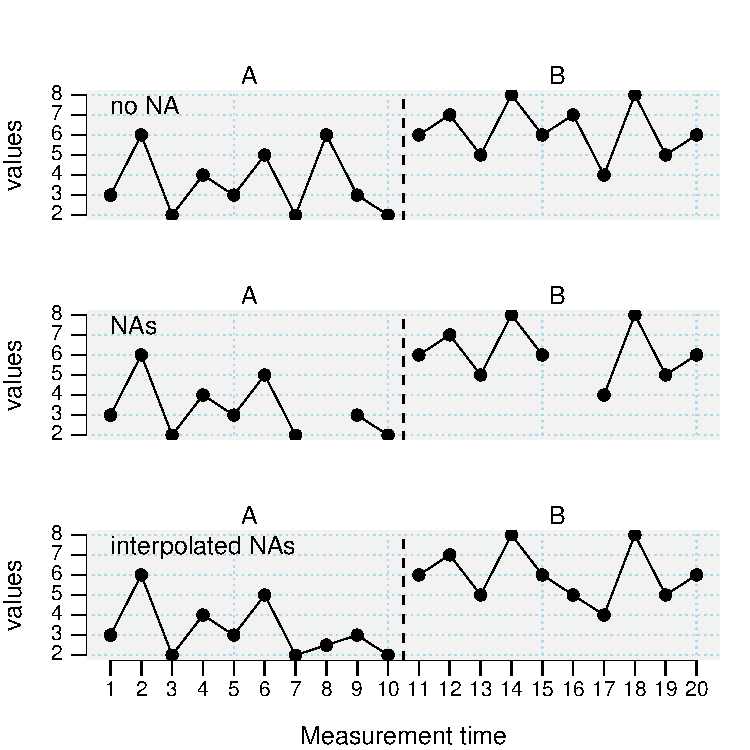
\includegraphics{./ch_describe_manipulate_files/figure-pdf/fillmissing_example-1.pdf}

}

\end{figure}

\begin{Shaded}
\begin{Highlighting}[]
\FunctionTok{overlap}\NormalTok{(ex)}
\end{Highlighting}
\end{Shaded}

\begin{verbatim}
Overlap Indices

Comparing phase 1 against phase 2 

             no NA  NAs interpolated NAs
Design         A-B  A-B              A-B
PND             40   33               30
PEM            100  100              100
PET            100  100              100
NAP             88   91               92
NAP rescaled    77   83               83
PAND            72   81               80
Tau_U         0.45 0.51             0.50
Base_Tau      0.59 0.64             0.64
Diff_mean     2.60 2.78             2.75
Diff_trend    0.02 0.11             0.12
SMD           1.65 1.96             2.02
Hedges_g      1.71 1.90             1.96
\end{verbatim}

\hypertarget{outlieranalysis}{%
\section{Outlieranalysis}\label{outlieranalysis}}

\begin{tcolorbox}[enhanced jigsaw, toprule=.15mm, colframe=quarto-callout-tip-color-frame, left=2mm, colback=white, breakable, bottomrule=.15mm, arc=.35mm, rightrule=.15mm, leftrule=.75mm, opacityback=0]
\begin{minipage}[t]{5.5mm}
\textcolor{quarto-callout-tip-color}{\faLightbulb}
\end{minipage}%
\begin{minipage}[t]{\textwidth - 5.5mm}
outlier(data, dvar, pvar, mvar, criteria = c(``MAD'',
``3.5''))\end{minipage}%
\end{tcolorbox}

\emph{scan} provides several methods for analyzing outliers. All of them
are implemented in the \texttt{outliers} function. Available methods are
the \textbf{standard deviation}, \textbf{mean average deviation},
\textbf{confidence intervals}, and \textbf{Cook's distance}. The
criteria argument takes a vector with two information, the first defines
the analyzing method (``SD'', ``MAD'', CI'', ``Cook'') and the second
the criteria. For ``SD'' the criteria is the number of standard
deviations (\textbf{sd}) from the mean of each phase for which a value
is not considered to be an outlier. For example,
\texttt{criteria\ =\ c("SD",2)} would identify every value exceeding two
\textbf{sd} above or below the mean as an outlier whereas \textbf{sd}
and mean refer to phase of a value. As this might be misleading
particularly for small samples Iglewicz and Hoaglin Iglewicz \& Hoaglin
(1993) recommend the use the much more robust median average deviation
(\textbf{MAD}) instead. The \textbf{MAD} is is constructed similar to
the \textbf{sd} but uses the median instead of the mean. Multiplying the
\textbf{MAD} by 1.4826 approximates the \textbf{sd} in a normal
distributed sample. This corrected MAD is applied in the
\texttt{outlier} function. A deviation of 3.5 times the corrected
\textbf{MAD} from the median is suggested to be an outlier. To use this
criterion set \texttt{criteria\ =\ c("MAD",\ 3.5)}.
\texttt{criteria\ =\ c("CI",\ 0.95)} takes exceeding the 95\% confidence
interval as the criteria for outliers. The Cook's distance method for
calculation outliers can be applied with a strict AB-phase design. in
that case, the Cook's distance analyses are based on a
piecewise-regression model. Most commonly, Cook's distance exceeding 4/n
is used as a criteria. This could be implemented setting `criteria =
c(``Cook'',``4/n'').

\begin{Shaded}
\begin{Highlighting}[]
\FunctionTok{outlier}\NormalTok{(exampleABC\_outlier, }\AttributeTok{criteria =} \FunctionTok{c}\NormalTok{(}\StringTok{"MAD"}\NormalTok{, }\FloatTok{3.5}\NormalTok{))}
\end{Highlighting}
\end{Shaded}

\begin{verbatim}
Outlier Analysis for Single-Case Data

Criteria: Exceeds 3.5 Mean Average Deviations

$Bernadette
  phase md mad   lower    upper
1     A 57   9 10.2981 103.7019
2     B 76   7 39.6763 112.3237
3     C 69  12  6.7308 131.2692

$Penny
  phase md mad   lower    upper
1     A 52   6 20.8654  83.1346
2     B 74  10 22.1090 125.8910
3     C 68   8 26.4872 109.5128

$Amy
  phase md mad   lower    upper
1     A 54   9  7.2981 100.7019
2     B 73  11 15.9199 130.0801
3     C 76  14  3.3526 148.6474

Case Bernadette : Dropped 3 
Case Penny : Dropped 2 
Case Amy : Dropped 3 
\end{verbatim}

\begin{Shaded}
\begin{Highlighting}[]
\CommentTok{\# Visualizing outliers with the plot function}
\NormalTok{res }\OtherTok{\textless{}{-}} \FunctionTok{outlier}\NormalTok{(exampleABC\_outlier, }\AttributeTok{criteria =} \FunctionTok{c}\NormalTok{(}\StringTok{"MAD"}\NormalTok{, }\FloatTok{3.5}\NormalTok{))}
\FunctionTok{plot}\NormalTok{(exampleABC\_outlier, }\AttributeTok{marks =}\NormalTok{ res, }\AttributeTok{style =} \StringTok{"annotate"}\NormalTok{, }\AttributeTok{ylim =} \FunctionTok{c}\NormalTok{(}\DecValTok{40}\NormalTok{,}\DecValTok{160}\NormalTok{))}
\end{Highlighting}
\end{Shaded}

\begin{figure}[H]

{\centering 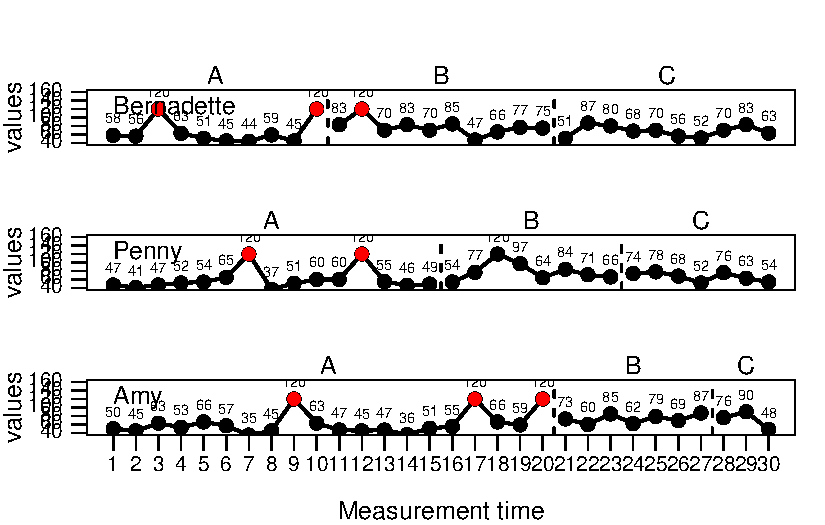
\includegraphics{./ch_describe_manipulate_files/figure-pdf/outlier-1.pdf}

}

\end{figure}

\hypertarget{smoothing-data}{%
\section{Smoothing data}\label{smoothing-data}}

\begin{tcolorbox}[enhanced jigsaw, toprule=.15mm, colframe=quarto-callout-tip-color-frame, left=2mm, colback=white, breakable, bottomrule=.15mm, arc=.35mm, rightrule=.15mm, leftrule=.75mm, opacityback=0]
\begin{minipage}[t]{5.5mm}
\textcolor{quarto-callout-tip-color}{\faLightbulb}
\end{minipage}%
\begin{minipage}[t]{\textwidth - 5.5mm}
smooth\_cases(data, dvar, mvar, FUN = ``movingMedian'', intensity =
NULL)\end{minipage}%
\end{tcolorbox}

The \texttt{smooth\_cases} function provides procedures to smooth
single-case data and eliminate noise. A moving average function (mean-
or median-based) replaces each data point by the average of the
surrounding data points step-by-step. A \emph{lag} defines the number of
measurements before and after the calculation is based on. So a lag-1
will take the average of the proceeding and following value and lag-2
the average of the two proceeding and two following measurements. With a
local regression function, each data point is regressed by its
surrounding data points. Here, the proportion of measurements
surrounding a value is usually defined. So an intensity of 0.2 will take
the surrounding 20\% of data as the basis for a regression.\\
The function returns am scdf with smoothed data points.

\begin{Shaded}
\begin{Highlighting}[]
\DocumentationTok{\#\# Use the three different smoothing functions and compare the results}
\NormalTok{berta\_mmd }\OtherTok{\textless{}{-}} \FunctionTok{smooth\_cases}\NormalTok{(Huber2014}\SpecialCharTok{$}\NormalTok{Berta)}
\NormalTok{berta\_mmn }\OtherTok{\textless{}{-}} \FunctionTok{smooth\_cases}\NormalTok{(Huber2014}\SpecialCharTok{$}\NormalTok{Berta, }\AttributeTok{FUN =} \StringTok{"movingMean"}\NormalTok{)}
\NormalTok{berta\_lre }\OtherTok{\textless{}{-}} \FunctionTok{smooth\_cases}\NormalTok{(Huber2014}\SpecialCharTok{$}\NormalTok{Berta, }\AttributeTok{FUN =} \StringTok{"localRegression"}\NormalTok{)}
\NormalTok{new\_study }\OtherTok{\textless{}{-}} \FunctionTok{c}\NormalTok{(Huber2014}\SpecialCharTok{$}\NormalTok{Berta, berta\_mmd, berta\_mmn, berta\_lre)}
\FunctionTok{names}\NormalTok{(new\_study) }\OtherTok{\textless{}{-}} \FunctionTok{c}\NormalTok{(}\StringTok{"Original"}\NormalTok{, }\StringTok{"Moving Median"}\NormalTok{, }\StringTok{"Moving Mean"}\NormalTok{, }\StringTok{"Local Regression"}\NormalTok{)}
\FunctionTok{plot}\NormalTok{(new\_study, }\AttributeTok{style =} \StringTok{"grid2"}\NormalTok{)}
\end{Highlighting}
\end{Shaded}

\begin{figure}[H]

{\centering 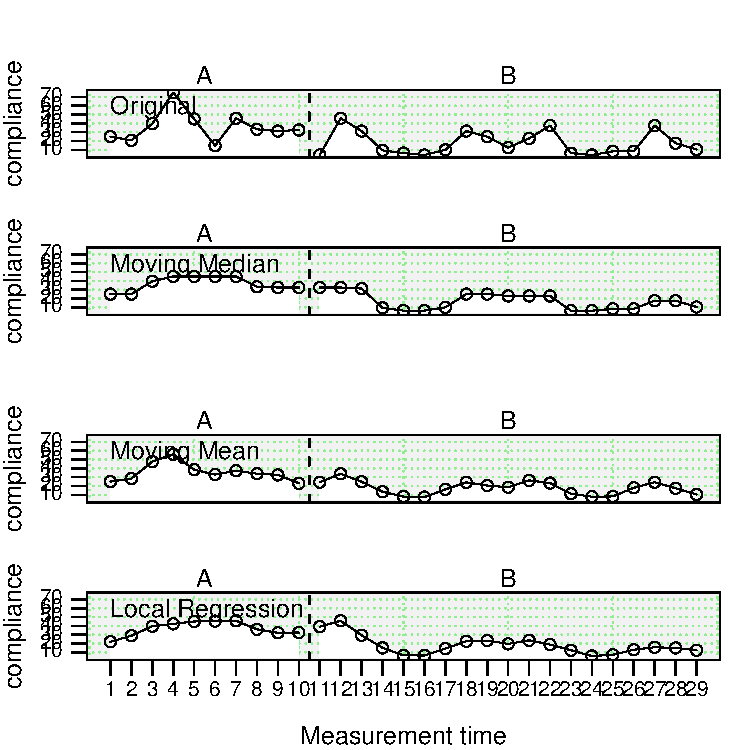
\includegraphics{./ch_describe_manipulate_files/figure-pdf/smooth_example-1.pdf}

}

\end{figure}

\hypertarget{overlapping-indices}{%
\chapter{Overlapping indices}\label{overlapping-indices}}

\hypertarget{overlap-overview}{%
\section{Overlap overview}\label{overlap-overview}}

\begin{tcolorbox}[enhanced jigsaw, toprule=.15mm, colframe=quarto-callout-tip-color-frame, left=2mm, colback=white, breakable, bottomrule=.15mm, arc=.35mm, rightrule=.15mm, leftrule=.75mm, opacityback=0]
\begin{minipage}[t]{5.5mm}
\textcolor{quarto-callout-tip-color}{\faLightbulb}
\end{minipage}%
\begin{minipage}[t]{\textwidth - 5.5mm}
overlap(data, dvar, pvar, mvar, decreasing = FALSE, phases = c(1,
2))\end{minipage}%
\end{tcolorbox}

\texttt{overlap} provides a table with some of the most important
overlap indices for each case of an \emph{scdf}. For calculating overlap
indicators it is important to know if a decrease or an increase of
values is expected between phases. By default \texttt{overlap} assumes
an increase in values. If the argument \texttt{decreasing\ =\ TRUE} is
set, calculation will be based on the assumption of decreasing values.

\begin{Shaded}
\begin{Highlighting}[]
\FunctionTok{overlap}\NormalTok{(exampleAB)}
\end{Highlighting}
\end{Shaded}

\begin{verbatim}
Overlap Indices

Comparing phase 1 against phase 2 

             Johanna Karolina  Anja
Design           A-B      A-B   A-B
PND              100       87    93
PEM              100      100   100
PET              100       93   100
NAP              100       97    98
NAP rescaled     100       93    96
PAND             100       90    90
Tau_U           0.77     0.78  0.64
Base_Tau        0.63     0.59  0.61
Diff_mean      19.53    21.67 20.47
Diff_trend      1.53     0.54  2.50
SMD             8.11     3.17  6.71
Hedges_g        2.35     2.26  2.87
\end{verbatim}

Overlap measures refer to a comparison of two phases within a
single-case data-set. By default, \texttt{overlap} compares the first to
the second phase.

\hypertarget{sec-select-phases}{%
\subsection{Select and recombine phases}\label{sec-select-phases}}

\begin{tcolorbox}[enhanced jigsaw, toprule=.15mm, colframe=quarto-callout-tip-color-frame, left=2mm, colback=white, breakable, bottomrule=.15mm, arc=.35mm, rightrule=.15mm, leftrule=.75mm, opacityback=0]
\begin{minipage}[t]{5.5mm}
\textcolor{quarto-callout-tip-color}{\faLightbulb}
\end{minipage}%
\begin{minipage}[t]{\textwidth - 5.5mm}
select\_phases(data, A, B)\end{minipage}%
\end{tcolorbox}

The \texttt{select\_phases()} function is needed if you like to compare
specific phases or even like to combine several phases.
\texttt{select\_phases()} is designed to work within a pipe structure.
So the first argument is an \emph{scdf} and it returns an \emph{scdf}.

\begin{Shaded}
\begin{Highlighting}[]
\NormalTok{scdf }\SpecialCharTok{\%\textgreater{}\%} \FunctionTok{select\_phases}\NormalTok{(}\AttributeTok{A =} \DecValTok{1}\NormalTok{, }\AttributeTok{B =} \DecValTok{3}\NormalTok{) }\SpecialCharTok{\%\textgreater{}\%}\NormalTok{ ...}
\end{Highlighting}
\end{Shaded}

\texttt{select\_phases()} has the arguments \texttt{A} and \texttt{B}.
Each argument takes a vector with the names or the numbers of the phases
to be selected. If you want to compare the first to the third phase you
can set \texttt{select\_phases(scdf,\ 1,3)}. If the phases of your case
are named `A', `B', and `C' you could alternatively set
\texttt{select\_phases(scdf,\ "A","C")}. It is also possible to compare
a combination of several cases against a combination of other phases.
Each of the two list-elements could contain more than one phase which
are concatenated with the \texttt{c} command. For example if you have an
ABAB-Design and like to compare the two A-phases against the two
B-phases \texttt{select\_phases(scdf,\ c(1,3),\ c(2,4)\ )} will do the
trick.

(As an alternative approach you can set the \texttt{phases} argument
within the \texttt{overlap()} function. This argument takes a list with
two elements where the first element defines the phases for the A-phase
and the second argument the phases for the B-phase.)

\begin{Shaded}
\begin{Highlighting}[]
\NormalTok{exampleA1B1A2B2 }\SpecialCharTok{\%\textgreater{}\%}
  \FunctionTok{select\_phases}\NormalTok{(}\FunctionTok{c}\NormalTok{(}\StringTok{"A1"}\NormalTok{,}\StringTok{"A2"}\NormalTok{), }\FunctionTok{c}\NormalTok{(}\StringTok{"B1"}\NormalTok{,}\StringTok{"B2"}\NormalTok{)) }\SpecialCharTok{\%\textgreater{}\%}
  \FunctionTok{overlap}\NormalTok{()}
\end{Highlighting}
\end{Shaded}

\begin{verbatim}
Overlap Indices

Comparing phase 1 against phase 2 

             Pawel Moritz Jannis
Design         A-B    A-B    A-B
PND             55     78     71
PEM            100    100    100
PET            100    100    100
NAP             94     97     98
NAP rescaled    89     94     97
PAND            82     85     90
Tau_U         0.45   0.46   0.38
Base_Tau      0.65   0.68   0.68
Diff_mean    12.25  13.58  15.27
Diff_trend   -0.05   0.00  -0.54
SMD           2.68   3.27   3.62
Hedges_g      2.07   2.72   2.98
\end{verbatim}

\begin{Shaded}
\begin{Highlighting}[]
\CommentTok{\# Alternatively:}
\CommentTok{\# overlap(exampleA1B1A2B2, phases = list( c("A1","A2"), c("B1","B2")))}
\end{Highlighting}
\end{Shaded}

\hypertarget{standardized-mean-differences}{%
\section{Standardized mean
differences}\label{standardized-mean-differences}}

\begin{tcolorbox}[enhanced jigsaw, toprule=.15mm, colframe=quarto-callout-tip-color-frame, left=2mm, colback=white, breakable, bottomrule=.15mm, arc=.35mm, rightrule=.15mm, leftrule=.75mm, opacityback=0]
\begin{minipage}[t]{5.5mm}
\textcolor{quarto-callout-tip-color}{\faLightbulb}
\end{minipage}%
\begin{minipage}[t]{\textwidth - 5.5mm}
smd(data, dvar, pvar, mvar, decreasing = FALSE, phases = c(1,
2))\end{minipage}%
\end{tcolorbox}

Standardized mean differences can be calculated in various ways. They
refer to the difference in the means of two phases. The \texttt{smd}
function provides an overview of the most common parameters for each
single-case:

\begin{Shaded}
\begin{Highlighting}[]
\FunctionTok{smd}\NormalTok{(exampleAB\_score)}
\end{Highlighting}
\end{Shaded}

\begin{verbatim}
Standardized mean differences

                            Christiano Lionel Neymar
mA                                2.70   3.10   2.30
mB                               15.35  15.35  15.60
sdA                               1.42   1.59   1.49
sdB                               2.13   1.60   2.19
sd cohen                          1.81   1.60   1.87
sd hedges                         1.93   1.60   1.99
Glass' delta                      8.92   7.68   8.90
Hedges' g                         6.54   7.67   6.68
Hedges' g correction              6.37   7.46   6.50
Hedges' g durlak correction       6.15   7.21   6.28
Cohen's d                         6.98   7.67   7.10
\end{verbatim}

\hypertarget{percentage-non-overlapping-data-pnd}{%
\section{Percentage non-overlapping data
(PND)}\label{percentage-non-overlapping-data-pnd}}

\begin{tcolorbox}[enhanced jigsaw, toprule=.15mm, colframe=quarto-callout-tip-color-frame, left=2mm, colback=white, breakable, bottomrule=.15mm, arc=.35mm, rightrule=.15mm, leftrule=.75mm, opacityback=0]
\begin{minipage}[t]{5.5mm}
\textcolor{quarto-callout-tip-color}{\faLightbulb}
\end{minipage}%
\begin{minipage}[t]{\textwidth - 5.5mm}
pnd(data, dvar, pvar, decreasing = FALSE, phases = c(``A'',
``B''))\end{minipage}%
\end{tcolorbox}

The percentage of non-overlapping data (PND) effect size measure was
described by Scruggs, Mastropieri, \& Casto (1987) . It is the
percentage of all data-points of the second phase of a single-case study
exceeding the maximum value of the first phase. In case you have a study
where you expect a decrease of values in the second phase, PND is
calculated as the percentage of data-point of the second phase below the
minimum of the first phase.

\begin{figure}

{\centering 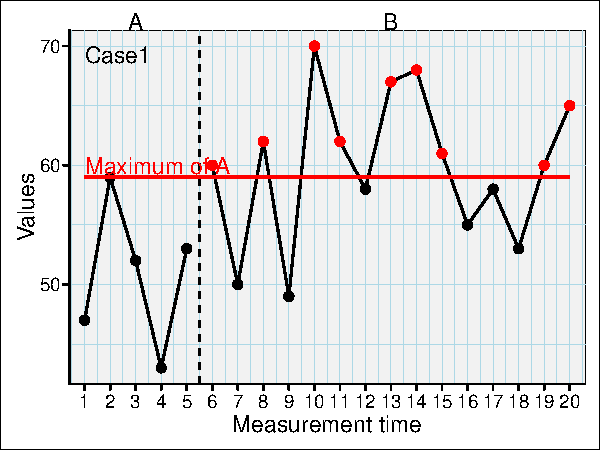
\includegraphics{./ch_overlapping_indices_files/figure-pdf/unnamed-chunk-9-1.pdf}

}

\caption{Illustration of PND. PND is 60\% as 9 out of 15 datapoints of
phase B are higher than the maximum of phase A}

\end{figure}

The function \texttt{pnd} provides the PND for each case as well as the
mean of all PNDs of that \emph{scdf}. When you expect decreasing values
set \texttt{decreasing\ =\ TRUE}. When there are more than two phases or
phases are not named A and B, use the \texttt{phases} argument as
described at the beginning of this chapter.

\begin{Shaded}
\begin{Highlighting}[]
\FunctionTok{pnd}\NormalTok{(exampleAB)}
\end{Highlighting}
\end{Shaded}

\begin{verbatim}
Percent Non-Overlapping Data

     Case    PND Total Exceeds
  Johanna   100%    15      15
 Karolina 86.67%    15      13
     Anja 93.33%    15      14

Mean  : 93.33 %
\end{verbatim}

\hypertarget{percentage-exceeding-the-median-pem}{%
\section{Percentage exceeding the median
(PEM)}\label{percentage-exceeding-the-median-pem}}

\begin{tcolorbox}[enhanced jigsaw, toprule=.15mm, colframe=quarto-callout-tip-color-frame, left=2mm, colback=white, breakable, bottomrule=.15mm, arc=.35mm, rightrule=.15mm, leftrule=.75mm, opacityback=0]
\begin{minipage}[t]{5.5mm}
\textcolor{quarto-callout-tip-color}{\faLightbulb}
\end{minipage}%
\begin{minipage}[t]{\textwidth - 5.5mm}
pem(data, dvar, pvar, decreasing = FALSE, binom.test = TRUE, chi.test =
FALSE, FUN = median, phases = c(1, 2), \ldots)\end{minipage}%
\end{tcolorbox}

The pem function returns the percentage of phase B data exceeding the
phase A median. Additionally, a binomial test against a 50/50
distribution is computed. Different measures of central tendency can be
addressed for alternative analyses.

\begin{figure}

{\centering 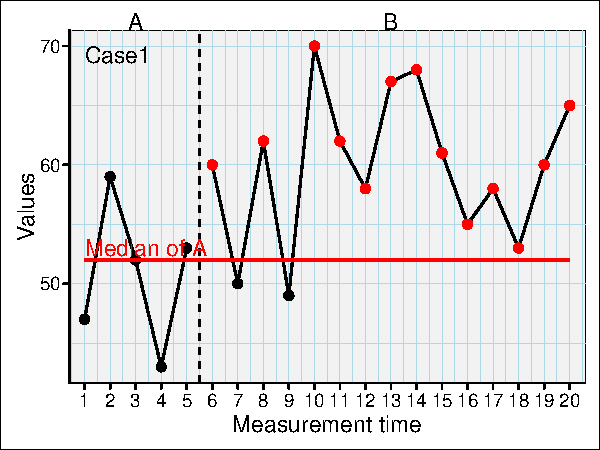
\includegraphics{./ch_overlapping_indices_files/figure-pdf/unnamed-chunk-12-1.pdf}

}

\caption{Illustration of PEM. PEM is 75\% as 13 out of 15 datapoints of
phase B are higher than the median of phase A}

\end{figure}

\begin{Shaded}
\begin{Highlighting}[]
\FunctionTok{pem}\NormalTok{(exampleAB)}
\end{Highlighting}
\end{Shaded}

\begin{verbatim}
Percent Exceeding the Median

         PEM positives total binom.p
Johanna  100        15    15       0
Karolina 100        15    15       0
Anja     100        15    15       0

Alternative hypothesis: true probability > 50%
\end{verbatim}

\hypertarget{percentage-exceeding-the-regression-trend-pet}{%
\section{Percentage exceeding the regression trend
(PET)}\label{percentage-exceeding-the-regression-trend-pet}}

\begin{tcolorbox}[enhanced jigsaw, toprule=.15mm, colframe=quarto-callout-tip-color-frame, left=2mm, colback=white, breakable, bottomrule=.15mm, arc=.35mm, rightrule=.15mm, leftrule=.75mm, opacityback=0]
\begin{minipage}[t]{5.5mm}
\textcolor{quarto-callout-tip-color}{\faLightbulb}
\end{minipage}%
\begin{minipage}[t]{\textwidth - 5.5mm}
pet(data, dvar, pvar, mvar, ci = 0.95, decreasing = FALSE, phases = c(1,
2))\end{minipage}%
\end{tcolorbox}

The pet function provides the percentage of phase B data points
exceeding the prediction based on the phase A trend. A binomial test
against a 50/50 distribution is computed. Furthermore, the percentage of
phase B data points exceeding the upper (or lower) 95 percent confidence
interval of the predicted progress is computed.

\begin{Shaded}
\begin{Highlighting}[]
\FunctionTok{pet}\NormalTok{(exampleAB)}
\end{Highlighting}
\end{Shaded}

\begin{verbatim}
Percent Exceeding the Trend

N cases =  3 

             PET binom.p  PET CI
Johanna  100.000       0  86.667
Karolina  93.333       0   0.000
Anja     100.000       0 100.000

Binom.test: alternative hypothesis: true probability > 50%
PET CI: Percent of values greater than upper 95% confidence threshold (greater 1.645*se above predicted value)
\end{verbatim}

\begin{figure}

{\centering 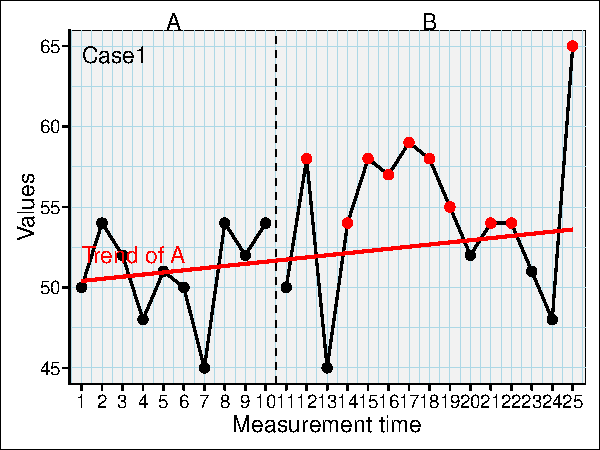
\includegraphics{./ch_overlapping_indices_files/figure-pdf/unnamed-chunk-16-1.pdf}

}

\caption{Illustration of PET. PET is 66.7\% as 10 out of 15 datapoints
of phase B are higher than the projected trend-line of phase A}

\end{figure}

\hypertarget{percentage-of-all-non-overlapping-data-pand}{%
\section{Percentage of all non-overlapping data
(PAND)}\label{percentage-of-all-non-overlapping-data-pand}}

\begin{tcolorbox}[enhanced jigsaw, toprule=.15mm, colframe=quarto-callout-tip-color-frame, left=2mm, colback=white, breakable, bottomrule=.15mm, arc=.35mm, rightrule=.15mm, leftrule=.75mm, opacityback=0]
\begin{minipage}[t]{5.5mm}
\textcolor{quarto-callout-tip-color}{\faLightbulb}
\end{minipage}%
\begin{minipage}[t]{\textwidth - 5.5mm}
pand(data, dvar, pvar, decreasing = FALSE, correction = TRUE, phases =
c(1, 2))\end{minipage}%
\end{tcolorbox}

The \texttt{pand} function calculates the percentage of all
non-overlapping data (Richard I. Parker, Hagan-Burke, \& Vannest, 2007),
an index to quantify a level increase (or decrease) in performance after
the onset of an intervention. The argument \texttt{correction\ =\ TRUE}
makes \texttt{pand} use a frequency matrix, which is corrected for ties.
A tie is counted as the half of a measurement in both phases. Set
\texttt{correction\ =\ FALSE} to use the uncorrected matrix, which is
not recommended.

\begin{Shaded}
\begin{Highlighting}[]
\FunctionTok{pand}\NormalTok{(exampleAB)}
\end{Highlighting}
\end{Shaded}

\begin{verbatim}
Percentage of all non-overlapping data

PAND =  93.3 %
Φ =  0.822  ; Φ² =  0.676 

Number of cases: 3 
Total measurements: 60  (in phase A: 15; in phase B: 45)
n overlapping data per case: 0, 2, 2
Total overlapping data: n = 4 ; percentage = 6.7 

2 x 2 Matrix of proportions
    % expected
    A   B   total
%    A  21.7    3.3 25
real B  3.3 71.7    75
 total  25  75

2 x 2 Matrix of counts
    expected
    A   B   total
     A  13  2   15
real B  2   43  45
 total  15  45


Note. Matrix is corrected for ties

Correlation based analysis:

z = 6.316, p = 0.000, τ = 0.822 
\end{verbatim}

PAND indicates nonoverlap between phase A and B data (like PND), but
uses all data and is therefore not based on one single (probably
unrepresentative) datapoint. Furthermore, PAND allows the comparison of
real and expected associations (Chi-square test) and estimation of the
effect size Phi, which equals Pearsons r for dichotomous data. Thus,
phi-Square is the amount of explained variance. The original procedure
for computing PAND does not account for ambivalent datapoints (ties).
The newer NAP overcomes this problem and has better precision-power
(Richard I. Parker, Vannest, \& Davis, 2011a).

\hypertarget{nonoverlap-of-all-pairs-nap}{%
\section{Nonoverlap of all pairs
(NAP)}\label{nonoverlap-of-all-pairs-nap}}

\begin{tcolorbox}[enhanced jigsaw, toprule=.15mm, colframe=quarto-callout-tip-color-frame, left=2mm, colback=white, breakable, bottomrule=.15mm, arc=.35mm, rightrule=.15mm, leftrule=.75mm, opacityback=0]
\begin{minipage}[t]{5.5mm}
\textcolor{quarto-callout-tip-color}{\faLightbulb}
\end{minipage}%
\begin{minipage}[t]{\textwidth - 5.5mm}
nap(data, dvar, pvar, decreasing = FALSE, phases = c(1,
2))\end{minipage}%
\end{tcolorbox}

The \texttt{nap} function calculates the nonoverlap of all pairs
(Richard I. Parker \& Vannest, 2009). NAP summarizes the overlap between
all pairs of phase A and phase B data points. If an increase of phase B
scores is expected, a non-overlapping pair has a higher phase B data
point. The NAP equals number of pairs showing no overlap / number of
pairs. Because NAP can only take values between 50 and 100 percent, a
rescaled and therefore more intuitive NAP (0-100\%) is also displayed.
NAP is equivalent to the the U-test and Wilcox rank sum test. Thus, a
Wilcox test is conducted and reported for each case.

\begin{Shaded}
\begin{Highlighting}[]
\FunctionTok{nap}\NormalTok{(exampleAB)}
\end{Highlighting}
\end{Shaded}

\begin{verbatim}
Nonoverlap of All Pairs

     Case NAP Rescaled Pairs Positives Ties   W       p
  Johanna 100      100    75        75    0 0.0 0.00062
 Karolina  97       93    75        72    1 2.5 0.00129
     Anja  98       96    75        73    1 1.5 0.00095
\end{verbatim}

\hypertarget{tau-u}{%
\section{Tau-U}\label{tau-u}}

\begin{tcolorbox}[enhanced jigsaw, toprule=.15mm, colframe=quarto-callout-tip-color-frame, left=2mm, colback=white, breakable, bottomrule=.15mm, arc=.35mm, rightrule=.15mm, leftrule=.75mm, opacityback=0]
\begin{minipage}[t]{5.5mm}
\textcolor{quarto-callout-tip-color}{\faLightbulb}
\end{minipage}%
\begin{minipage}[t]{\textwidth - 5.5mm}
tau\_u(data, dvar, pvar, tau\_method = ``b'', method = ``complete'',
phases = c(1, 2), meta\_method = ``random'', ci = 0.95,
continuity\_correction = FALSE)\end{minipage}%
\end{tcolorbox}

The \emph{Tau-U} statistic has been proposed by Richard I. Parker,
Vannest, Davis, \& Sauber (2011b) and is one of the more broadly used
approach for reporting effect sizes of single case data. Unfortunately,
various and ambiguous implementations of Tau-U exist (Brossart, Laird,
\& Armstrong, 2018; Pustejovsky, 2016). The \texttt{tau\_u} function
tries to cover several of these implementation. It takes a \emph{scdf}
and returns Tau-U calculations for each single-case within that file.
Additionally, an overall Tau-U value is calculated for all cases based
on a meta-analysis.

Several arguments an be set to define how Tau-U should be calculated. By
setting the argument \texttt{method\ =\ "parker"}, Tau-U is calculated
as described in Richard I. Parker et al. (2011b). This procedure could
lead to Tau-U values above 1 and below -1 which are difficult to
interpret. \texttt{method\ =\ "complete}, which is the default, applies
a correction that keeps the values within the -1 to 1 range and should
be more appropriate. In the original method proposed by Richard I.
Parker et al. (2011b) data, calculations are based on Kendall's Tau A
which does not correct for ties. Alternatively, Kendall's Tau B has a
correction for Tau in the presence of ties. The \texttt{tau\_method}`
can be set to decide on the tau method to use \texttt{"a"} for Kendall's
Tau A and \texttt{"b"}` for Kendall's Tau B.

Here is an example with setting that reconstruct the values from the
original example in Richard I. Parker, Vannest, Davis, \& Sauber (2011c)
:

\begin{Shaded}
\begin{Highlighting}[]
\FunctionTok{tau\_u}\NormalTok{(Parker2011, }\AttributeTok{method =} \StringTok{"parker"}\NormalTok{, }\AttributeTok{tau\_method =} \StringTok{"a"}\NormalTok{, }\AttributeTok{continuity\_correction =} \ConstantTok{FALSE}\NormalTok{, }\AttributeTok{ci =} \ConstantTok{NA}\NormalTok{)}
\end{Highlighting}
\end{Shaded}

\begin{verbatim}
Tau-U
Method: parker 
Applied Kendall's Tau-a

Case: Case1 
                              Tau SE_Tau    Z     p
A vs. B                     0.800  0.408 1.96 0.050
A vs. B - Trend A           0.650  0.480 1.35 0.175
A vs. B + Trend B           0.767  0.320 2.40 0.016
A vs. B + Trend B - Trend A 0.556  0.266 2.08 0.037
\end{verbatim}

A different implementation of the method (provided at
\href{http://www.singlecaseresearch.org/calculators/tau-u}{http://www.singlecaseresearch.org/calculators/tau-u)})
uses Kendall's Tau B:

\begin{Shaded}
\begin{Highlighting}[]
\FunctionTok{tau\_u}\NormalTok{(exampleAB}\SpecialCharTok{$}\NormalTok{Johanna, }\AttributeTok{method =} \StringTok{"parker"}\NormalTok{, }\AttributeTok{tau\_method =} \StringTok{"b"}\NormalTok{, }\AttributeTok{continuity\_correction =} \ConstantTok{FALSE}\NormalTok{)}
\end{Highlighting}
\end{Shaded}

\begin{verbatim}
Tau-U
Method: parker 
Applied Kendall's Tau-b

Case: Johanna 
                              Tau SE_Tau    Z     p
A vs. B                     1.000  0.306 3.27 0.001
A vs. B - Trend A           0.592  0.184 3.22 0.001
A vs. B + Trend B           0.786  0.166 4.75 0.000
A vs. B + Trend B - Trend A 0.765  0.163 4.71 0.000
\end{verbatim}

A different online calculator created by Rumen Manolov is available at
\url{https://manolov.shinyapps.io/Overlap/} it applies an R code
developed by Kevin Tarlow for caluclating Tau-U. This setting will
replicated results from this approach:

\begin{Shaded}
\begin{Highlighting}[]
\FunctionTok{tau\_u}\NormalTok{(exampleAB}\SpecialCharTok{$}\NormalTok{Johanna, }\AttributeTok{method =} \StringTok{"complete"}\NormalTok{, }\AttributeTok{tau\_method =} \StringTok{"a"}\NormalTok{, }\AttributeTok{continuity\_correction =} \ConstantTok{FALSE}\NormalTok{)}
\end{Highlighting}
\end{Shaded}

\begin{verbatim}
Tau-U
Method: complete 
Applied Kendall's Tau-a

Case: Johanna 
                              Tau SE_Tau    Z     p
A vs. B                     1.000  0.306 3.27 0.001
A vs. B - Trend A           0.882  0.363 2.43 0.015
A vs. B + Trend B           0.806  0.171 4.70 0.000
A vs. B + Trend B - Trend A 0.763  0.162 4.70 0.000
\end{verbatim}

The standard return of the \texttt{tau\_u} function does not display all
calculations. If you like to have more details, apply the \texttt{print}
function with the additional argument \texttt{complete\ =\ TRUE}.

\begin{Shaded}
\begin{Highlighting}[]
\FunctionTok{tau\_u}\NormalTok{(exampleAB}\SpecialCharTok{$}\NormalTok{Johanna) }\SpecialCharTok{\%\textgreater{}\%} \FunctionTok{print}\NormalTok{(}\AttributeTok{complete =} \ConstantTok{TRUE}\NormalTok{)}
\end{Highlighting}
\end{Shaded}

\begin{verbatim}
Tau-U
Method: complete 
Applied Kendall's Tau-b
95% CIs for tau are reported.

Case: Johanna 
                            pairs pos neg ties   S   D   Tau CI lower CI upper
A vs. B                        75  75   0    0  75  75 1.000    0.401    1.599
Trend A                        10   5   5    0   0  10 0.000      NaN      NaN
Trend B                       105  87  17    1  70 104 0.670    0.291    1.049
A vs. B - Trend A              85  80   5    0  75 127 0.592    0.232    0.951
A vs. B + Trend B             180 162  17    1 145 184 0.786    0.462    1.111
A vs. B + Trend B - Trend A   190 167  22    1 145 189 0.765    0.447    1.084
                             SD_S VAR_S SE_Tau    Z     p
A vs. B                     22.91 525.0  0.306 3.27 0.001
Trend A                      4.08  16.7    NaN 0.00 1.000
Trend B                     20.21 408.3  0.193 3.46 0.001
A vs. B - Trend A           23.26 541.2  0.184 3.22 0.001
A vs. B + Trend B           30.53 932.4  0.166 4.75 0.000
A vs. B + Trend B - Trend A 30.81 949.0  0.163 4.71 0.000
\end{verbatim}

When you provide multiple single-cases to the \texttt{tau-u} function,
it will calculate a Tau-U table for each case and an overall
calculation. The overall Tau-U value is the average of all Tau-U values
weighted by their standard error. You can choose between a random- and a
fixed-effect approach for the meta-analyses
(\texttt{meta\_method\ =\ "random"} or \texttt{"fixed"}).

\begin{Shaded}
\begin{Highlighting}[]
\FunctionTok{tau\_u}\NormalTok{(exampleAB)}
\end{Highlighting}
\end{Shaded}

\begin{verbatim}
Tau-U
Method: complete 
Applied Kendall's Tau-b
95% CIs for tau are reported.

Overall Tau-U
Meta-anlysis model: random effect

                       Model Tau_U     se CI lower CI upper    z        p
                     A vs. B 0.969 0.1772    0.622    1.316 5.47 4.54e-08
           A vs. B - Trend A 0.590 0.1064    0.381    0.798 5.54 3.04e-08
           A vs. B + Trend B 0.740 0.0960    0.552    0.928 7.71 1.29e-14
 A vs. B + Trend B - Trend A 0.731 0.0942    0.546    0.915 7.75 9.09e-15

Case: Johanna 
                              Tau SE_Tau    Z     p
A vs. B                     1.000  0.306 3.27 0.001
A vs. B - Trend A           0.592  0.184 3.22 0.001
A vs. B + Trend B           0.786  0.166 4.75 0.000
A vs. B + Trend B - Trend A 0.765  0.163 4.71 0.000

Case: Karolina 
                              Tau SE_Tau    Z     p
A vs. B                     0.940  0.308 3.06 0.002
A vs. B - Trend A           0.554  0.184 3.01 0.003
A vs. B + Trend B           0.805  0.166 4.85 0.000
A vs. B + Trend B - Trend A 0.783  0.163 4.81 0.000

Case: Anja 
                              Tau SE_Tau    Z     p
A vs. B                     0.966  0.308 3.14 0.002
A vs. B - Trend A           0.624  0.186 3.36 0.001
A vs. B + Trend B           0.626  0.167 3.74 0.000
A vs. B + Trend B - Trend A 0.642  0.164 3.91 0.000
\end{verbatim}

\hypertarget{baseline-corrected-tau}{%
\section{Baseline corrected tau}\label{baseline-corrected-tau}}

\begin{tcolorbox}[enhanced jigsaw, toprule=.15mm, colframe=quarto-callout-tip-color-frame, left=2mm, colback=white, breakable, bottomrule=.15mm, arc=.35mm, rightrule=.15mm, leftrule=.75mm, opacityback=0]
\begin{minipage}[t]{5.5mm}
\textcolor{quarto-callout-tip-color}{\faLightbulb}
\end{minipage}%
\begin{minipage}[t]{\textwidth - 5.5mm}
corrected\_tau(data, dvar, pvar, mvar, phases = c(1, 2), alpha = 0.05,
continuity = FALSE, repeated = FALSE)\end{minipage}%
\end{tcolorbox}

This method has been proposed by Tarlow (2016). The baseline data are
checked for a significant autocorrelation (based on Kendalls Tau). If
so, a non-parameteric Theil-Sen regression is applied for the baseline
data where the dependent values are regressed on the measurement time.
The resulting slope information is then used to predict data of the
B-phase. The dependent variable is now corrected for this baseline trend
and the residuals of the Theil-Sen regression are taken for further
calculations. Finally, Kendalls tau is calculated for the dependent
variable and the dichotomous phase variable. The function here provides
two extensions to this procedure: The alternative Siegel repeated median
regression is applied when \texttt{repeated\ =\ TRUE} (Siegel, 1982) and
a continuity correction is applied when \texttt{continuity\ =\ TRUE}
(both not the defaults).

Here is a replication of an example provided by Tarlow (2016) :

\begin{verbatim}
Warning: Removed 11 row(s) containing missing values (geom_path).
\end{verbatim}

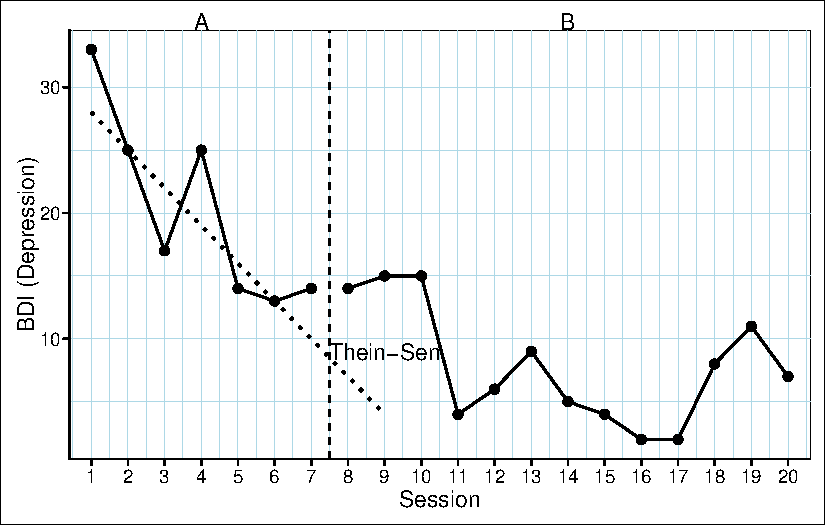
\includegraphics{./ch_overlapping_indices_files/figure-pdf/bctau-example-1.pdf}

\begin{verbatim}
Baseline corrected tau

Method: Theil-Sen regression
Continuity correction not applied.

                           tau     z     p
Baseline autocorrelation -0.75 -2.31  <.05
Uncorrected tau          -0.58 -2.98  <.01
Baseline corrected tau    0.69  3.57 <.001

Baseline correction should be applied.
\end{verbatim}

\hypertarget{reliable-change-index}{%
\section{Reliable change index}\label{reliable-change-index}}

\begin{tcolorbox}[enhanced jigsaw, toprule=.15mm, colframe=quarto-callout-tip-color-frame, left=2mm, colback=white, breakable, bottomrule=.15mm, arc=.35mm, rightrule=.15mm, leftrule=.75mm, opacityback=0]
\begin{minipage}[t]{5.5mm}
\textcolor{quarto-callout-tip-color}{\faLightbulb}
\end{minipage}%
\begin{minipage}[t]{\textwidth - 5.5mm}
rci(data, dvar, pvar, rel, ci = 0.95, graph = FALSE, phases = c(1,
2))\end{minipage}%
\end{tcolorbox}

Basically, the reliable change index (rci) depicts if a post-test is
above a pre-test value. Based on the reliability of the measurements and
the standard-deviation the standard error is calculated. The mean
difference between phase-A and phase-B is divided by the standard-error.
Several authors proposed refined methods for calculating the rci.

The \texttt{rci} function computes three indices of reliable change
(Wise, 2004) and corresponding descriptive statistics.

\begin{Shaded}
\begin{Highlighting}[]
\FunctionTok{rci}\NormalTok{(exampleAB}\SpecialCharTok{$}\NormalTok{Johanna, }\AttributeTok{rel =} \FloatTok{0.8}\NormalTok{, }\AttributeTok{graph =} \ConstantTok{TRUE}\NormalTok{)}
\end{Highlighting}
\end{Shaded}

\begin{figure}[H]

{\centering 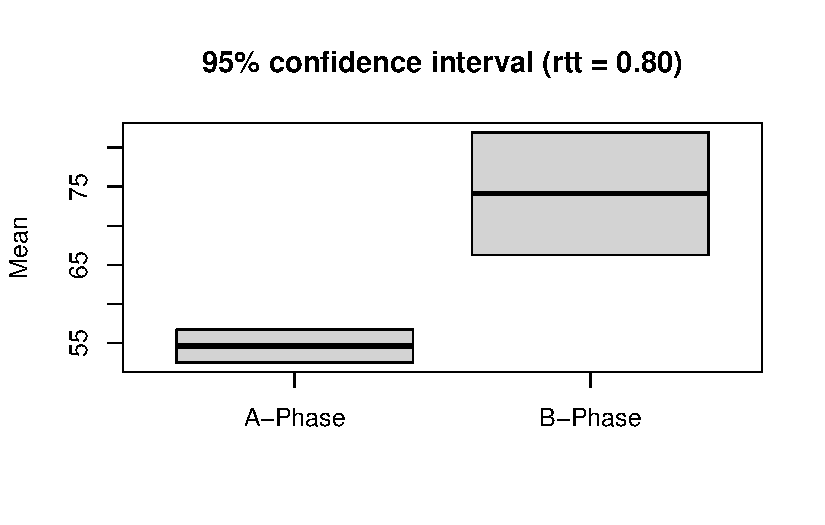
\includegraphics{./ch_overlapping_indices_files/figure-pdf/unnamed-chunk-28-1.pdf}

}

\end{figure}

\begin{verbatim}
Reliable Change Index

Mean Difference =  19.53333 
Standardized Difference =  1.678301 

Descriptives:
         n     mean       SD       SE
A-Phase  5 54.60000 2.408319 1.077033
B-Phase 15 74.13333 8.943207 3.999524

Reliability =  0.8 

95 % Confidence Intervals:
           Lower    Upper
A-Phase 52.48905 56.71095
B-Phase 66.29441 81.97226

Reliable Change Indices:
                             RCI
Jacobson et al.         18.13624
Christensen and Mendoza 12.82426
Hageman and Arrindell   18.49426
\end{verbatim}

\hypertarget{piecewise-linear-regressions}{%
\chapter{Piecewise linear
regressions}\label{piecewise-linear-regressions}}

In a piecewise-regression analysis (sometimes called segmented
regression) a dataset is split at a specific break point and regression
parameters (intercept and slopes) are calculated separately for data
before and after the break point. This is done because we assume that at
the break point a qualitative change happens affecting intercept and
slope. This approach lends itself perfectly to analyze single-case data
which are from a statistical point of view time-series data segmented
into phases. A general model for single-case data based on the piecewise
regression approach has been suggested by Huitema and McKean Huitema \&
Mckean (2000). They refer to two-phase single-case designs with a
pre-intervention phase containing some measurements before the start of
the intervention (A-phase) and an intervention phase containing
measurements beginning at the intervention's start and lasting
throughout the intervention (B-phase).

In this model, four parameters predict the outcome at a specific
measurement point:

\begin{enumerate}
\def\labelenumi{\arabic{enumi}.}
\item
  The performance at the beginning of the study (\textbf{intercept}),
\item
  a developmental effect leading to a continuous increase throughout all
  measurements (\textbf{trend effect}),
\item
  an intervention effect leading to an immediate and constant increase
  in performance (\textbf{level effect}), and
\item
  a second intervention effect that evolves continuously with the
  beginning of the intervention (\textbf{slope effect}).
\end{enumerate}

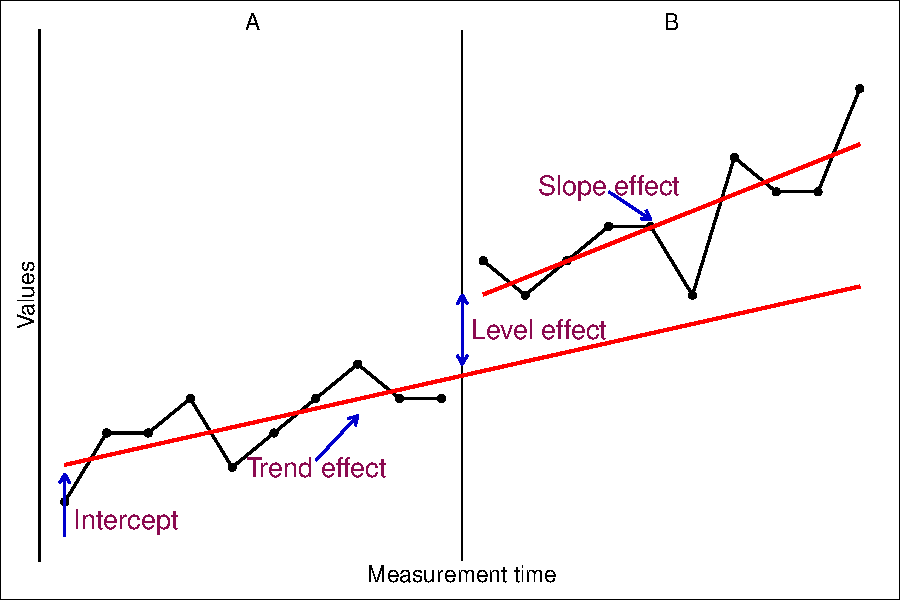
\includegraphics{./ch_piecewise_regression_files/figure-pdf/figure_plm-1.pdf}

\emph{scan} provides an implementation based on this
piecewise-regression approach. Though the original model is extended by
several factors:

\begin{itemize}
\tightlist
\item
  multiple phase designs
\item
  additional (control) variables
\item
  autoregression modeling
\item
  logistic, binomial, and poisson distributed dependent variables and
  error terms
\item
  multivariate analyzes for analyzing the effect of an intervention on
  more than one outcome variable.
\end{itemize}

\hypertarget{the-basic-plm-function}{%
\section{The basic plm function}\label{the-basic-plm-function}}

\begin{tcolorbox}[enhanced jigsaw, toprule=.15mm, colframe=quarto-callout-tip-color-frame, left=2mm, colback=white, breakable, bottomrule=.15mm, arc=.35mm, rightrule=.15mm, leftrule=.75mm, opacityback=0]
\begin{minipage}[t]{5.5mm}
\textcolor{quarto-callout-tip-color}{\faLightbulb}
\end{minipage}%
\begin{minipage}[t]{\textwidth - 5.5mm}
plm(data, dvar, pvar, mvar, AR = 0, model = ``W'', family =
``gaussian'', trend = TRUE, level = TRUE, slope = TRUE, contrast =
``first'', formula = NULL, update = NULL, na.action = na.omit,
r\_squared = TRUE, var\_trials = NULL, dvar\_percentage = FALSE,
\ldots)\end{minipage}%
\end{tcolorbox}

The basic function for applying a regression analyzes to a single-case
dataset is \texttt{plm}. This function analyzes one single-case. In its
simplest way, \texttt{plm} takes one argument with an \emph{scdf} object
and it returns a full piecewise-regression analyzes.

\begin{Shaded}
\begin{Highlighting}[]
\FunctionTok{plm}\NormalTok{(exampleAB}\SpecialCharTok{$}\NormalTok{Johanna)}
\end{Highlighting}
\end{Shaded}

\begin{verbatim}
Piecewise Regression Analysis

Dummy model: W first

Fitted a gaussian distribution.
F(3, 16) = 28.69; p = 0.000; R² = 0.843; Adjusted R² = 0.814

                   B   2.5%  97.5%    SE      t     p delta R²
Intercept     54.400 46.776 62.024 3.890 13.986 0.000         
Trend mt       0.100 -3.012  3.212 1.588  0.063 0.951   0.0000
Level phase B  7.858 -3.542 19.258 5.816  1.351 0.195   0.0179
Slope phase B  1.525 -1.642  4.692 1.616  0.944 0.359   0.0087

Autocorrelations of the residuals
 lag    cr
   1 -0.32
   2 -0.13
   3 -0.01

Formula: values ~ 1 + mt + phaseB + interB
\end{verbatim}

\hypertarget{dummy-model}{%
\subsection{Dummy model}\label{dummy-model}}

The \texttt{model} argument is used to code the \emph{dummy variable}.
This \emph{dummy variable} is used to compute the slope and level
effects of the \emph{phase} variable.\\
The \emph{phase} variable is categorical, identifying the phase of each
measurement. Typically, categorical variables are implemented by means
of dummy variables. In a piecewise regression model two phase effects
have to be estimated: a level effect and a slope effect. The level
effect is implemented quite straight forward: for each phase beginning
with the second phase a new dummy variable is created with values of
zero for all measurements except the measurements of the phase in focus
where values of one are set.

\begin{longtable}[]{@{}rlrr@{}}
\toprule()
mt & phase & values & level\_B \\
\midrule()
\endhead
1 & A & 3 & 0 \\
2 & A & 6 & 0 \\
3 & A & 4 & 0 \\
4 & A & 7 & 0 \\
5 & B & 5 & 1 \\
6 & B & 3 & 1 \\
7 & B & 4 & 1 \\
8 & B & 6 & 1 \\
9 & B & 3 & 1 \\
\bottomrule()
\end{longtable}

For estimating the \emph{slope effect} of each phase, another kind of
dummy variables have to be created. Like the dummy variables for level
effects the values are set to zero for all measurements except the ones
of the phase in focus. Here, values start to increase with every
measurement until the end of the phase.\\
Various suggestions have been made regarding the way in which these
values increase. The \emph{B\&L-B} model starts with a one at the first
measurement of the phase and increases with every measurement while the
\emph{H-M} model starts with a zero.

\begin{longtable}[]{@{}rlrrrr@{}}
\toprule()
mt & phase & values & level & slope B\&L-M & slope H-M \\
\midrule()
\endhead
1 & A & 3 & 0 & 0 & 0 \\
2 & A & 6 & 0 & 0 & 0 \\
3 & A & 4 & 0 & 0 & 0 \\
4 & A & 7 & 0 & 0 & 0 \\
5 & B & 5 & 1 & 1 & 0 \\
6 & B & 3 & 1 & 2 & 1 \\
7 & B & 4 & 1 & 3 & 2 \\
8 & B & 6 & 1 & 4 & 3 \\
9 & B & 3 & 1 & 5 & 4 \\
\bottomrule()
\end{longtable}

Applying the \emph{H-M} model will give you a ``pure'' level-effect
while the \emph{B\&L-B} model will provide an estimation of the
level-effect that is actually the level-effect plus on times the
slope-effect (as the the model assumes that the slope variable is
\emph{1} at the first measurement of the B-phase). For most studies, the
\emph{H-M} model is more appropriate.

Still, we have to be aware of another aspect. Usually, measurement-times
in single-case designs are coded as starting with \emph{1} and
increasing in integers (e.g., 1, 2, 3, \ldots). At the same time, the
estimation of the trend-effect is based on the measurement-time
variable. In that case, the estimation of the model intercept (usually
interpreted as the value at the start of the study) actually depicts the
estimation of the start value plus one times the trend-effect.
Therefore, I implemented the \emph{W} model (since scan version
\texttt{0.54.4}). Here, the trend-effect is estimated for a
measurement-time variable that starts with \emph{0}. As a result the
intercept will then represent the estimated value at the first
measurement fo the study. The \emph{W} model handles the slope
estimation the same way as the \emph{H-M} model. Since scan version
\texttt{0.54.4} the \emph{W} model is the default.

\hfill\break

\begin{longtable}[]{@{}lrrrrrrr@{}}
\toprule()
phase & values & level & mt B\&L-M and H-M & slope B\&L-M & slope H-M &
mt W & slope W \\
\midrule()
\endhead
A & 3 & 0 & 1 & 0 & 0 & 0 & 0 \\
A & 6 & 0 & 2 & 0 & 0 & 1 & 0 \\
A & 4 & 0 & 3 & 0 & 0 & 2 & 0 \\
A & 7 & 0 & 4 & 0 & 0 & 3 & 0 \\
B & 5 & 1 & 5 & 1 & 0 & 4 & 0 \\
B & 3 & 1 & 6 & 2 & 1 & 5 & 1 \\
B & 4 & 1 & 7 & 3 & 2 & 6 & 2 \\
B & 6 & 1 & 8 & 4 & 3 & 7 & 3 \\
B & 3 & 1 & 9 & 5 & 4 & 8 & 4 \\
\bottomrule()
\end{longtable}

\hypertarget{designs-with-more-than-two-phases-setting-the-right-contrasts}{%
\subsection{Designs with more than two phases: Setting the right
contrasts}\label{designs-with-more-than-two-phases-setting-the-right-contrasts}}

With single-case studies with more than two phases it gets a bit more
complicated. Applying the afore described models to three phases would
result in a comparison of each phase to the first phase (usually the A
Phase). That is, regression weights and significance tests will depict
differences of each phase to the values of phase A. This might be OK
depending on what you are interested in. Another usual application is to
compare the effects of a phase to the preceding one.\\
Since scan version \texttt{0.54.4} plm allows to set a contrast
argument. \texttt{contrast\ =\ "first"}` (the default) will compare all
slope and level-effects to the values in the first phase.
\texttt{contrast\ =\ "preceding"}` will compare the slope and
level-effects to the preceding phase. (Note: Prior to scan version
\texttt{0.54.4} you had to set \texttt{model\ =\ "JW"} which is
identical to \texttt{model\ =\ "B\&L-B",\ contrast\ =\ "preceding"}`).

For the \emph{preceding contrast}, the dummy variable for the
level-effect is set to zero for all phases preceding the phase in focus
and set to one for all remaining measurements. Similar, the dummy
variable for the slope-effect is set to zero for all phases preceding
the one in focus and starts with one for the first measurement of the
target phase and increases until the last measurement of the case.

\begin{longtable}[]{@{}lrrrrr@{}}
\toprule()
phase & values & level\_B & level\_C & slope\_B & slope\_C \\
\midrule()
\endhead
A & 3 & 0 & 0 & 0 & 0 \\
A & 6 & 0 & 0 & 0 & 0 \\
A & 4 & 0 & 0 & 0 & 0 \\
A & 7 & 0 & 0 & 0 & 0 \\
B & 5 & 1 & 0 & 1 & 0 \\
B & 3 & 1 & 0 & 2 & 0 \\
B & 4 & 1 & 0 & 3 & 0 \\
B & 6 & 1 & 0 & 4 & 0 \\
B & 3 & 1 & 0 & 5 & 0 \\
C & 7 & 1 & 1 & 6 & 1 \\
C & 5 & 1 & 1 & 7 & 2 \\
C & 6 & 1 & 1 & 8 & 3 \\
C & 4 & 1 & 1 & 9 & 4 \\
C & 8 & 1 & 1 & 10 & 5 \\
\bottomrule()
\end{longtable}

\hypertarget{adjusting-the-model}{%
\subsection{Adjusting the model}\label{adjusting-the-model}}

\begin{Shaded}
\begin{Highlighting}[]
\NormalTok{example }\OtherTok{\textless{}{-}} \FunctionTok{scdf}\NormalTok{(}
   \AttributeTok{values =} \FunctionTok{c}\NormalTok{(}\DecValTok{55}\NormalTok{, }\DecValTok{58}\NormalTok{, }\DecValTok{53}\NormalTok{, }\DecValTok{50}\NormalTok{, }\DecValTok{52}\NormalTok{, }\DecValTok{55}\NormalTok{, }\DecValTok{68}\NormalTok{, }\DecValTok{68}\NormalTok{, }\DecValTok{81}\NormalTok{, }\DecValTok{67}\NormalTok{, }\DecValTok{78}\NormalTok{, }\DecValTok{73}\NormalTok{, }\DecValTok{72}\NormalTok{, }\DecValTok{78}\NormalTok{, }\DecValTok{81}\NormalTok{, }\DecValTok{78}\NormalTok{, }\DecValTok{71}\NormalTok{, }\DecValTok{85}\NormalTok{, }\DecValTok{80}\NormalTok{, }\DecValTok{76}\NormalTok{),}
   \AttributeTok{phase\_design =} \FunctionTok{c}\NormalTok{(}\AttributeTok{A =} \DecValTok{5}\NormalTok{, }\AttributeTok{B =} \DecValTok{15}\NormalTok{)}
\NormalTok{)}

\FunctionTok{plm}\NormalTok{(example)}
\end{Highlighting}
\end{Shaded}

\begin{verbatim}
Piecewise Regression Analysis

Dummy model: W first

Fitted a gaussian distribution.
F(3, 16) = 21.36; p = 0.000; R² = 0.800; Adjusted R² = 0.763

                   B   2.5%  97.5%    SE      t     p delta R²
Intercept     56.400 48.070 64.730 4.250 13.270 0.000         
Trend mt      -1.400 -4.801  2.001 1.735 -0.807 0.432   0.0081
Level phase B 16.967  4.510 29.424 6.356  2.670 0.017   0.0890
Slope phase B  2.500 -0.961  5.961 1.766  1.416 0.176   0.0250

Autocorrelations of the residuals
 lag    cr
   1 -0.28
   2  0.05
   3 -0.11

Formula: values ~ 1 + mt + phaseB + interB
\end{verbatim}

The piecewise regression reveals a significant level effect and two non
significant effects for trend and slope. In a further analyses we would
like to put the slope effect out of the equation. There are several ways
to do this. The easiest way is the to set the \texttt{slope} argument to
\texttt{FALSE}.

\begin{Shaded}
\begin{Highlighting}[]
\FunctionTok{plm}\NormalTok{(example, }\AttributeTok{slope =} \ConstantTok{FALSE}\NormalTok{)}
\end{Highlighting}
\end{Shaded}

\begin{verbatim}
Piecewise Regression Analysis

Dummy model: W first

Fitted a gaussian distribution.
F(2, 17) = 29.30; p = 0.000; R² = 0.775; Adjusted R² = 0.749

                   B   2.5%  97.5%    SE      t     p delta R²
Intercept     51.572 46.455 56.690 2.611 19.752 0.000         
Trend mt       1.014  0.364  1.664 0.332  3.057 0.007   0.1236
Level phase B 10.329  1.674 18.983 4.416  2.339 0.032   0.0724

Autocorrelations of the residuals
 lag    cr
   1 -0.07
   2  0.06
   3 -0.17

Formula: values ~ 1 + mt + phaseB
\end{verbatim}

In the resulting estimations the trend and level effects are now
significant. The model estimated a trend effect of 1.01 points per
measurement time and a level effect of 10.33 points. That is, with the
beginning of the intervention (the B-phase) the score increases by 15.38
points (5 x 1.01 + 10.33).

\hypertarget{adding-additional-predictors}{%
\subsection{Adding additional
predictors}\label{adding-additional-predictors}}

In more complex analyses additional predictors can be included in the
piecewise regression model.

To do this, we have to change the regression formula `manually' by
applying the \texttt{update} argument. The \texttt{update} argument
allows to change the underlying regression formula. To add a new
variable named for example \texttt{newVar}, set
\texttt{update\ =\ .\textasciitilde{}.\ +\ newVar}. The
\texttt{.\textasciitilde{}.} part takes the internally build formula and
\texttt{+\ newVar} adds a variable named \texttt{newVar} to the
equation.

\begin{Shaded}
\begin{Highlighting}[]
\FunctionTok{plm}\NormalTok{(exampleAB\_add, }\AttributeTok{update =}\NormalTok{ .}\SpecialCharTok{\textasciitilde{}}\NormalTok{. }\SpecialCharTok{+}\NormalTok{ cigarrets)}
\end{Highlighting}
\end{Shaded}

\begin{verbatim}
Piecewise Regression Analysis

Dummy model: W first

Fitted a gaussian distribution.
F(4, 35) = 5.87; p = 0.001; R² = 0.402; Adjusted R² = 0.333

                            B   2.5%  97.5%    SE      t     p delta R²
Intercept              48.971 43.387 54.555 2.849 17.189 0.000         
Trend day               0.392 -0.221  1.005 0.313  1.253 0.218   0.0269
Level phase Medication  3.459 -3.382 10.301 3.490  0.991 0.328   0.0168
Slope phase Medication -0.294 -0.972  0.384 0.346 -0.850 0.401   0.0124
cigarrets              -0.221 -1.197  0.755 0.498 -0.443 0.660   0.0034

Autocorrelations of the residuals
 lag    cr
   1  0.20
   2 -0.19
   3 -0.16

Formula: wellbeing ~ day + phaseMedication + interMedication + cigarrets
\end{verbatim}

The formula has two parts divided by a tilde. Left of the tilde is the
variable to be predicted and right of it the predictors. A \texttt{1}
indicates the intercept, the variable \texttt{mt} estimates the trend
effect, \texttt{phaseB} the level effect of the B-phase and the variable
\texttt{interB} the slope effect of the B-phase. If \texttt{formula} is
not explicitly defined it is set to
\texttt{formula\ =\ values\ \textasciitilde{}\ 1\ +\ mt\ +\ phaseB\ +\ interB}
(assuming an AB-design) to estimate the full piecewise regression model.

\hypertarget{to-be-written-modelling-autoregression}{%
\subsection{\texorpdfstring{\[to be written\] Modelling
autoregression}{to be written Modelling autoregression}}\label{to-be-written-modelling-autoregression}}

\begin{Shaded}
\begin{Highlighting}[]
\FunctionTok{autocorr}\NormalTok{(Grosche2011)}
\end{Highlighting}
\end{Shaded}

\begin{verbatim}
Autocorrelations

Eva 
 Phase Lag 1 Lag 2 Lag 3
     A -0.04 -0.56 -0.01
     B  0.46  0.10  0.16
   all  0.48  0.13  0.24

Georg 
 Phase Lag 1 Lag 2 Lag 3
     A  0.51 -0.01 -0.13
     B -0.01 -0.02 -0.14
   all  0.40  0.15 -0.12

Olaf 
 Phase Lag 1 Lag 2 Lag 3
     A  0.64  0.29 -0.24
     B -0.45 -0.20  0.16
   all  0.35  0.12 -0.09
\end{verbatim}

\hypertarget{to-be-written-multivariate-piecewise-regression}{%
\section{\texorpdfstring{\[to be written\] Multivariate piecewise
regression}{to be written Multivariate piecewise regression}}\label{to-be-written-multivariate-piecewise-regression}}

\begin{tcolorbox}[enhanced jigsaw, toprule=.15mm, colframe=quarto-callout-tip-color-frame, left=2mm, colback=white, breakable, bottomrule=.15mm, arc=.35mm, rightrule=.15mm, leftrule=.75mm, opacityback=0]
\begin{minipage}[t]{5.5mm}
\textcolor{quarto-callout-tip-color}{\faLightbulb}
\end{minipage}%
\begin{minipage}[t]{\textwidth - 5.5mm}
mplm(data, dvar, mvar, pvar, model = ``W'', contrast = ``first'', trend
= TRUE, level = TRUE, slope = TRUE, formula = NULL, update = NULL,
na.action = na.omit, \ldots)\end{minipage}%
\end{tcolorbox}

\begin{Shaded}
\begin{Highlighting}[]
\FunctionTok{mplm}\NormalTok{(exampleAB\_add, }\AttributeTok{dvar =} \FunctionTok{c}\NormalTok{(}\StringTok{"wellbeing"}\NormalTok{, }\StringTok{"depression"}\NormalTok{))}
\end{Highlighting}
\end{Shaded}

\begin{verbatim}
Multivariate piecewise linear model

Dummy model: W first

Coefficients: 
                       wellbeing depression
(Intercept)               48.417      4.200
day                        0.379      0.114
Level Phase Medication     3.588     -0.945
Slope Phase Medication    -0.275     -0.165

Formula: y ~ 1 + day + phaseMedication + interMedication

Type III MANOVA Tests: Pillai test statistic
                       Df test stat approx F num Df den Df Pr(>F)    
(Intercept)             1     0.915    188.9      2     35 <2e-16 ***
day                     1     0.055      1.0      2     35   0.38    
Level Phase Medication  1     0.033      0.6      2     35   0.56    
Slope Phase Medication  1     0.039      0.7      2     35   0.50    
---
Signif. codes:  0 '***' 0.001 '**' 0.01 '*' 0.05 '.' 0.1 ' ' 1

The following variables were used in this analysis:
'wellbeing/ depression' as dependent variable, 'phase' as phase variable, and 'day' as measurement-time variable.
\end{verbatim}

\hypertarget{multilevel-plm-analyses}{%
\section{Multilevel plm analyses}\label{multilevel-plm-analyses}}

\begin{tcolorbox}[enhanced jigsaw, toprule=.15mm, colframe=quarto-callout-tip-color-frame, left=2mm, colback=white, breakable, bottomrule=.15mm, arc=.35mm, rightrule=.15mm, leftrule=.75mm, opacityback=0]
\begin{minipage}[t]{5.5mm}
\textcolor{quarto-callout-tip-color}{\faLightbulb}
\end{minipage}%
\begin{minipage}[t]{\textwidth - 5.5mm}
hplm(data, dvar, pvar, mvar, model = ``W'', contrast = ``first'', method
= ``ML'', control = list(opt = ``optim''), random.slopes = FALSE,
lr.test = FALSE, ICC = TRUE, trend = TRUE, level = TRUE, slope = TRUE,
fixed = NULL, random = NULL, update.fixed = NULL, data.l2 = NULL,
\ldots)\end{minipage}%
\end{tcolorbox}

Multilevel analyses can take the piecewise-regression approach even
further. It allows for

\begin{itemize}
\tightlist
\item
  analyzing the effects between phases for multiple single-cases at once
\item
  describing variability between subjects regarding these effects, and
\item
  introducing variables and factors for explaining the differences.
\end{itemize}

The basic function for applying a multilevel piecewise regression
analysis is \texttt{hplm}. The \texttt{hplm} function is similar to the
\texttt{plm} function, so I recommend that you get familar with
\texttt{plm} before applying an \texttt{hplm}.

Here is a simple example:

\begin{Shaded}
\begin{Highlighting}[]
\FunctionTok{hplm}\NormalTok{(exampleAB\_50)}
\end{Highlighting}
\end{Shaded}

\begin{verbatim}
Hierarchical Piecewise Linear Regression

Estimation method ML 
Dummy model: W first
50 Cases

ICC = 0.287; L = 339.0; p = 0.000

Fixed effects (values ~ 1 + mt + phaseB + interB)

                   B    SE   df      t p
Intercept     48.398 1.484 1328 32.611 0
Trend mt       0.579 0.116 1328  5.006 0
Level phase B 14.038 0.655 1328 21.436 0
Slope phase B  0.902 0.119 1328  7.588 0

Random effects (~1 | case)

          EstimateSD
Intercept      9.970
Residual       5.285
\end{verbatim}

Here is an example inlcuding random slopes:

\begin{Shaded}
\begin{Highlighting}[]
\FunctionTok{hplm}\NormalTok{(exampleAB\_50, }\AttributeTok{random.slopes =} \ConstantTok{TRUE}\NormalTok{)}
\end{Highlighting}
\end{Shaded}

\begin{verbatim}
Hierarchical Piecewise Linear Regression

Estimation method ML 
Dummy model: W first
50 Cases

ICC = 0.287; L = 339.0; p = 0.000

Fixed effects (values ~ 1 + mt + phaseB + interB)

                   B    SE   df      t p
Intercept     48.211 1.398 1328 34.497 0
Trend mt       0.621 0.113 1328  5.516 0
Level phase B 13.872 0.894 1328 15.513 0
Slope phase B  0.864 0.116 1328  7.433 0

Random effects (~1 + mt + phaseB + interB | case)

              EstimateSD
Intercept          9.352
Trend mt           0.096
Level phase B      4.537
Slope phase B      0.126
Residual           4.974
\end{verbatim}

\hypertarget{sec-add-l2}{%
\subsection{Adding additional L2-variables}\label{sec-add-l2}}

\begin{tcolorbox}[enhanced jigsaw, toprule=.15mm, colframe=quarto-callout-tip-color-frame, left=2mm, colback=white, breakable, bottomrule=.15mm, arc=.35mm, rightrule=.15mm, leftrule=.75mm, opacityback=0]
\begin{minipage}[t]{5.5mm}
\textcolor{quarto-callout-tip-color}{\faLightbulb}
\end{minipage}%
\begin{minipage}[t]{\textwidth - 5.5mm}
add\_l2(data, data\_l2, cvar = ``case'')\end{minipage}%
\end{tcolorbox}

In some analyses researchers want to investigate whether attributes of
the individuals contribute to the effectiveness of an intervention. For
example might an intervention on mathematical abilities be less
effective for student with a migration background due to too much
language related material within the training. Such analyses can also be
conducted with \emph{scan}. Therefore, we need to define a new
\emph{data frame} including the relevant information of the subjects of
the single-case studies we want to analyze. This \emph{data frame}
consists of a variable labeled \texttt{case} which has to correspond to
the case names of the \emph{scfd} and further variables with attributes
of the subjects. To build a \emph{data frame} we can use the R function
\texttt{data.frame}.

\begin{Shaded}
\begin{Highlighting}[]
\NormalTok{L2 }\OtherTok{\textless{}{-}} \FunctionTok{data.frame}\NormalTok{(}
  \AttributeTok{case =} \FunctionTok{c}\NormalTok{(}\StringTok{"Antonia"}\NormalTok{,}\StringTok{"Theresa"}\NormalTok{, }\StringTok{"Charlotte"}\NormalTok{, }\StringTok{"Luis"}\NormalTok{, }\StringTok{"Bennett"}\NormalTok{, }\StringTok{"Marie"}\NormalTok{), }
  \AttributeTok{age =} \FunctionTok{c}\NormalTok{(}\DecValTok{16}\NormalTok{, }\DecValTok{13}\NormalTok{, }\DecValTok{13}\NormalTok{, }\DecValTok{10}\NormalTok{, }\DecValTok{5}\NormalTok{, }\DecValTok{14}\NormalTok{), }
  \AttributeTok{sex =} \FunctionTok{c}\NormalTok{(}\StringTok{"f"}\NormalTok{,}\StringTok{"f"}\NormalTok{,}\StringTok{"f"}\NormalTok{,}\StringTok{"m"}\NormalTok{,}\StringTok{"m"}\NormalTok{,}\StringTok{"f"}\NormalTok{)}
\NormalTok{)}
\NormalTok{L2}
\end{Highlighting}
\end{Shaded}

\begin{verbatim}
       case age sex
1   Antonia  16   f
2   Theresa  13   f
3 Charlotte  13   f
4      Luis  10   m
5   Bennett   5   m
6     Marie  14   f
\end{verbatim}

Multilevel analyses require a high number of Level 2 units. The exact
number depends on the complexity of the analyses, the size of the
effects, the number of level 1 units, and the variability of the
residuals. But surely we need at least about 30 level 2 units. In a
single-case design that is, we need at least 30 single-cases (subjects)
within the study. After setting the level 2 data frame we can merge it
to the \emph{scdf} with the \texttt{add\_l2()} function (alternatively,
we can use the \texttt{data.l2} argument of the \texttt{hplm} function).
Then we have to specify the regression function using the
\texttt{update.fixed} argument. The level 2 variables can be added just
like any other additional variable. For example, we have added a level 2
data-set with the two variables \texttt{sex} and \texttt{age}.
\texttt{update} could be construed of the level 1 piecewise regression
model \texttt{.\textasciitilde{}.} plus the additional level 2 variables
of interest \texttt{+\ sex\ +\ age}. The complete argument is
\texttt{update.fixed\ =\ .\textasciitilde{}.\ +\ sex\ +\ age}. This
analyses will estimate a main effect of sex and age on the overall
performance. In case we want to analyze an interaction between the
intervention effects and for example the sex of the subject we have to
add an additional interaction term (a cross-level interaction). An
interaction is defined with a colon. So \texttt{sex:phase} indicates an
interaction of sex and the level effect in the single case study. The
complete formula now is
\texttt{update.fixed\ =\ .\textasciitilde{}.\ +\ sex\ +\ age\ +\ sex:phase}.

\emph{scan} includes an example single-case study with 50 subjects
\texttt{example50} and an additional level 2 data-set
\texttt{example50.l2}. Here are the first 10 cases of
\texttt{example50.l2}.

\begin{longtable}[]{@{}llr@{}}
\toprule()
case & sex & age \\
\midrule()
\endhead
Roman & m & 12 \\
Brennen & m & 10 \\
Ismael & m & 13 \\
Donald & m & 11 \\
Ricardo & m & 13 \\
Izayah & m & 11 \\
Ignacio & m & 12 \\
Xavier & m & 12 \\
Arian & m & 10 \\
Paul & m & 10 \\
\bottomrule()
\end{longtable}

Analyzing the data with \texttt{hplm} could look like this:

\begin{Shaded}
\begin{Highlighting}[]
\NormalTok{exampleAB\_50 }\SpecialCharTok{\%\textgreater{}\%}
  \FunctionTok{add\_l2}\NormalTok{(exampleAB\_50.l2) }\SpecialCharTok{\%\textgreater{}\%}
  \FunctionTok{hplm}\NormalTok{(}\AttributeTok{update.fixed =}\NormalTok{ .}\SpecialCharTok{\textasciitilde{}}\NormalTok{. }\SpecialCharTok{+}\NormalTok{ sex }\SpecialCharTok{+}\NormalTok{ age)}
\end{Highlighting}
\end{Shaded}

\begin{verbatim}
Hierarchical Piecewise Linear Regression

Estimation method ML 
Dummy model: W first
50 Cases

ICC = 0.287; L = 339.0; p = 0.000

Fixed effects (values ~ mt + phaseB + interB + sex + age)

                   B     SE   df      t     p
Intercept     44.878 11.926 1328  3.763 0.000
Trend mt       0.581  0.116 1328  5.026 0.000
Level phase B 14.023  0.655 1328 21.405 0.000
Slope phase B  0.900  0.119 1328  7.569 0.000
sexm          -6.440  2.727   47 -2.362 0.022
age            0.603  1.073   47  0.562 0.577

Random effects (~1 | case)

          EstimateSD
Intercept      9.446
Residual       5.284
\end{verbatim}

\begin{Shaded}
\begin{Highlighting}[]
\CommentTok{\# Alternatively:}
\CommentTok{\# hplm(exampleAB\_50, data.l2 = exampleAB\_50.l2, update.fixed = .\textasciitilde{}. + sex + age)}
\end{Highlighting}
\end{Shaded}

\texttt{sex} is a factor with the levels \texttt{f} and \texttt{m}. So
\texttt{sexm} is the effect of being male on the overall performance.
\texttt{age} does not seem to have any effect. So we drop \texttt{age}
out of the equation and add an interaction of sex and phase to see
whether the \texttt{sex} effect is due to a weaker impact of the
intervention on males.

\begin{Shaded}
\begin{Highlighting}[]
\NormalTok{exampleAB\_50 }\SpecialCharTok{\%\textgreater{}\%}
  \FunctionTok{add\_l2}\NormalTok{(exampleAB\_50.l2) }\SpecialCharTok{\%\textgreater{}\%}
  \FunctionTok{hplm}\NormalTok{(}\AttributeTok{update.fixed =}\NormalTok{ .}\SpecialCharTok{\textasciitilde{}}\NormalTok{. }\SpecialCharTok{+}\NormalTok{ sex }\SpecialCharTok{+}\NormalTok{ sex}\SpecialCharTok{:}\NormalTok{phaseB)}
\end{Highlighting}
\end{Shaded}

\begin{verbatim}
Hierarchical Piecewise Linear Regression

Estimation method ML 
Dummy model: W first
50 Cases

ICC = 0.287; L = 339.0; p = 0.000

Fixed effects (values ~ mt + phaseB + interB + sex + phaseB:sex)

                        B    SE   df       t    p
Intercept          48.573 1.968 1327  24.676 0.00
Trend mt            0.609 0.109 1327   5.573 0.00
Level phase B      17.726 0.684 1327  25.922 0.00
Slope phase B       0.884 0.112 1327   7.868 0.00
sexm               -0.593 2.741   48  -0.216 0.83
Level phase B:sexm -7.732 0.609 1327 -12.699 0.00

Random effects (~1 | case)

          EstimateSD
Intercept      9.494
Residual       4.989
\end{verbatim}

Now the interaction \texttt{phase:sexm} is significant and the main
effect is no longer relevant. It looks like the intervention effect is
\(7.7\) points lower for male subjects. While the level-effect is
\(17.7\) points for female subjects it is \(17.7\) - \(7.7\) = \(10\)
for males.

\hypertarget{randomization-tests}{%
\chapter{Randomization tests}\label{randomization-tests}}

\begin{tcolorbox}[enhanced jigsaw, toprule=.15mm, colframe=quarto-callout-tip-color-frame, left=2mm, colback=white, breakable, bottomrule=.15mm, arc=.35mm, rightrule=.15mm, leftrule=.75mm, opacityback=0]
\begin{minipage}[t]{5.5mm}
\textcolor{quarto-callout-tip-color}{\faLightbulb}
\end{minipage}%
\begin{minipage}[t]{\textwidth - 5.5mm}
rand\_test(data, dvar, pvar, statistic = ``Mean B-A'', number = 500,
complete = FALSE, limit = 5, startpoints = NA, exclude.equal = FALSE,
graph = FALSE, output = ``c'', phases = c(``A'', ``B''), seed =
NULL)\end{minipage}%
\end{tcolorbox}

The \texttt{rand\_test} function computes a randomization test for
single or multiple baseline single-case data. The function is based on
an algorithm from the SCRT package (Bulté \& Onghena, 2008, 2009), but
rewritten and extended.

The basic idea of a randomization thest is to think counter factually
``Assuming the phase had no influence of the measured data: what would
the difference between the phases of my case be, if I would have started
phase B at a different time?''. Considering the possible differences
between the phases under the assumption that the phase had no influence,
how likely are the real phase differences of the original case?

Therefore, a number of new cases are generated with a random start of
each phase. That is, these new cases have the same data as the original
case but different starting points for each phase. Now, a specific
\emph{statistic} (e.g., the mean difference between the phase A and
phase B data) is calculated for each new case. When enough random cases
are generated, we also generate a series of new statistic values
(e.g.~mean differences). The statistic for the original case is now
compared to this new statistic values. The percentile of the original
statistic within the new generated statistic values is the probability
of the original statistic under the assumption of a random distribution
of starting points of each phase. This percentile is returned as the
\emph{p-value} of the randomization test analyses.

\begin{figure}

{\centering 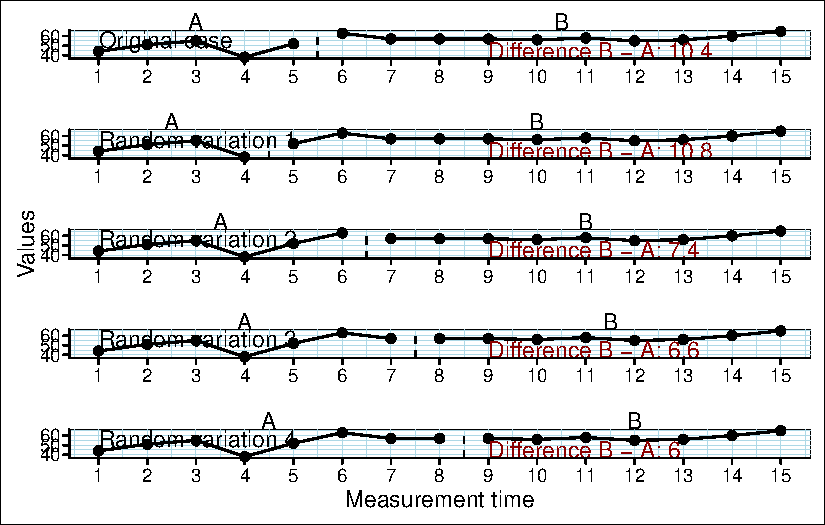
\includegraphics{./ch_randomization_test_files/figure-pdf/fig-ex-rand-test-1.pdf}

}

\caption{\label{fig-ex-rand-test}Illustration of a randomization test}

\end{figure}

\hypertarget{arguments-of-the-rand_test-function}{%
\section{\texorpdfstring{Arguments of the \texttt{rand\_test()}
function}{Arguments of the rand\_test() function}}\label{arguments-of-the-rand_test-function}}

The \texttt{statsitics} argument defines the statistic on which the
comparison of the phases is based on. The following comparisons are
possible:

\begin{itemize}
\tightlist
\item
  ``Mean A-B'': Uses the difference between the mean of phase A and the
  mean of phase B. * This is appropriate if a decrease of scores is
  expected for phase B.
\item
  ``Mean B-A'': Uses the difference between the mean of phase B and the
  mean of phase A. This is appropriate if an increase of scores is
  expected for phase B.
\item
  ``Mean \textbar A-B\textbar{}'': Uses the absolute value of the
  difference between the means of phases A and B.
\item
  ``Median A-B'': The same as ``Mean A-B'', but based on the median.
\item
  ``Median B-A'': The same as ``Mean B-A'', but based on the median.
\end{itemize}

\emph{number}\\
Sample size of the randomization distribution. The exactness of the
p-value can not exceed 1/number (i.e., number = 100 results in p-values
with an exactness of one percent). Default is number = 500. For faster
processing use number = 100. For more precise p-values set number =
1000.

\emph{complete}\\
If TRUE, the distribution is based on a complete permutation of all
possible starting combinations. This setting overwrites the number
Argument. The default setting is FALSE.

\emph{limit}\\
Minimal number of data points per phase in the sample. The first number
refers to the A-phase and the second to the B-phase (e.g., limit = c(5,
3)). If only one number is given, this number is applied to both phases.
Default is limit = 5.

\emph{startpoints}\\
Alternative to the limit-parameter, startpoints exactly defines the
possible start points of phase B (e.g., startpoints = 4:9 restricts the
phase B start points to measurements 4 to 9. startpoints overwrite the
limit-parameter.

\emph{exclude.equal}\\
If set to FALSE, which is the default, random distribution values equal
to the observed distribution are counted as null-hypothesis conform.
That is, they decrease the probability of rejecting the null-hypothesis
(increase the p-value). exclude.equal should be set to TRUE if you
analyse one single-case design (not a multiple baseline data set) to
reach a sufficient power. But be aware, that it increases the chance of
an alpha-error.

\emph{graph}\\
If set TRUE, a histogram of the resulting distribution is plotted.

\emph{phases}\\
A vector of two characters or numbers indicating the two phases that
should be compared. E.g., phases = c(``A'',``C'') or phases = c(2,4) for
comparing the second and the fourth phase. Phases could be combined by
providing a list with two elements. E.g., phases = list(A = c(1,3), B =
c(2,4)) will compare phases 1 and 3 (as A) against 2 and 4 (as B).
Default is phases = c(``A'',``B'').

\hypertarget{exanple}{%
\section{Exanple}\label{exanple}}

\begin{Shaded}
\begin{Highlighting}[]
\FunctionTok{rand\_test}\NormalTok{(exampleAB, }\AttributeTok{graph =} \ConstantTok{TRUE}\NormalTok{)}
\end{Highlighting}
\end{Shaded}

\begin{figure}[H]

{\centering 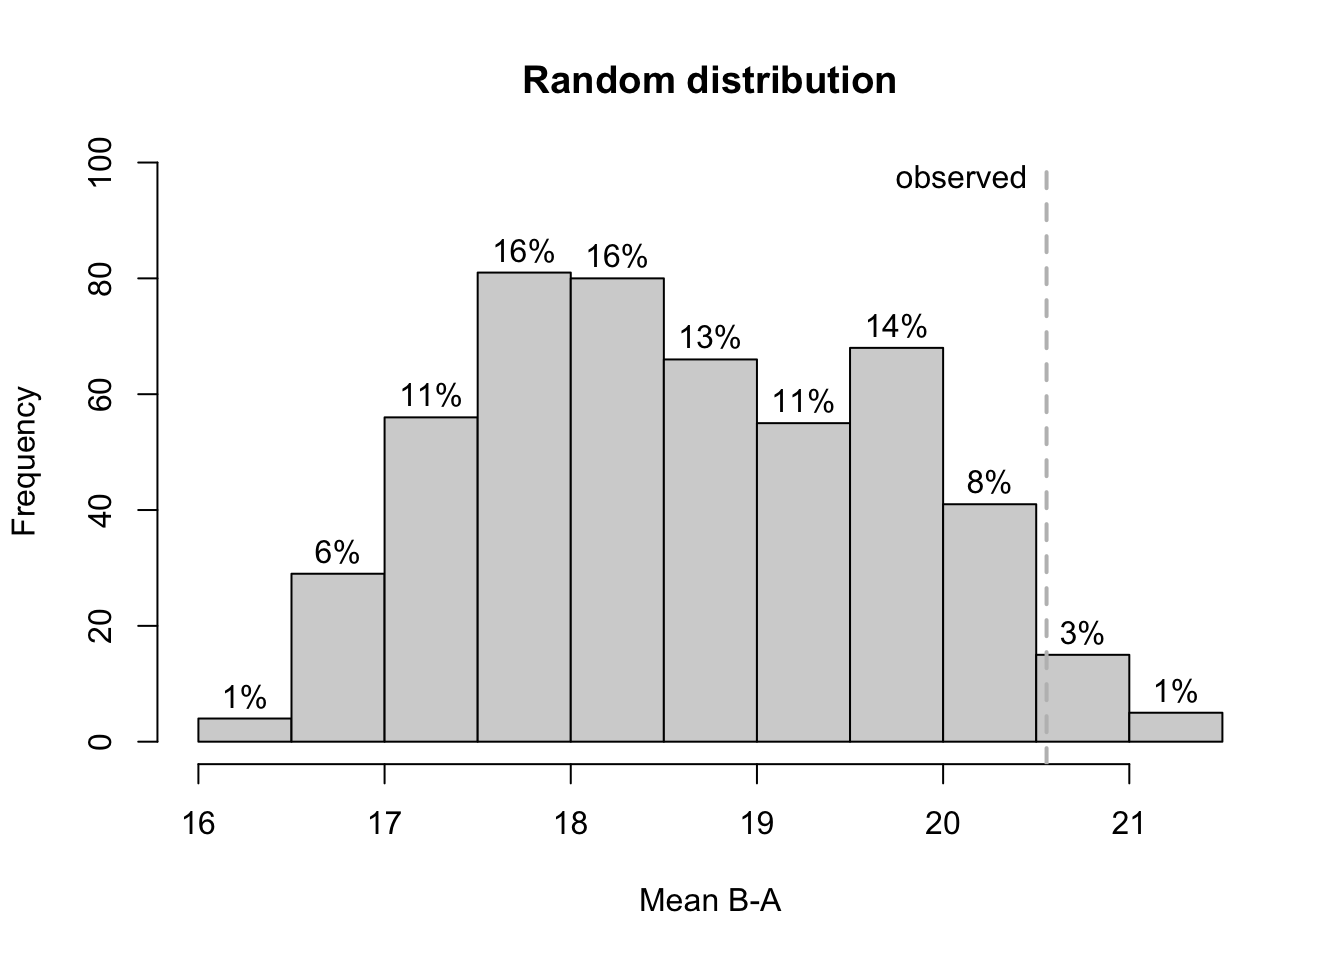
\includegraphics{./ch_randomization_test_files/figure-pdf/rand-1.pdf}

}

\end{figure}

\begin{verbatim}
Randomization Test

Test for 3 cases.

Comparing phase A against phase B 
Statistic:  Mean B-A 

Minimal length of each phase: A = 5 , B = 5 
Observed statistic =  20.55556 

Distribution based on a random sample of all 1331 possible combinations.
n   =  500 
M   =  18.5764 
SD  =  1.116712 
Min =  16.16243 
Max =  21.02897 

Probability of observed statistic based on distribution:
p   =  0.028 

Shapiro-Wilk Normality Test: W = 0.973; p = 0.000  (Hypothesis of normality rejected)

Probabilty of observed statistic based on the assumption of normality:
z = 1.7723, p = 0.0382 (single sided)
\end{verbatim}

\hypertarget{power-analyses-scan-version-0.54-or-later}{%
\chapter{Power analyses (scan version 0.54 or
later)}\label{power-analyses-scan-version-0.54-or-later}}

\begin{tcolorbox}[enhanced jigsaw, toprule=.15mm, colframe=quarto-callout-tip-color-frame, left=2mm, colback=white, breakable, bottomrule=.15mm, arc=.35mm, rightrule=.15mm, leftrule=.75mm, opacityback=0]
\begin{minipage}[t]{5.5mm}
\textcolor{quarto-callout-tip-color}{\faLightbulb}
\end{minipage}%
\begin{minipage}[t]{\textwidth - 5.5mm}
power\_test(design, method = c(``plm\_level'', ``rand'', ``tauU''),
effect = ``level'', n\_sim = 100, design\_is\_one\_study = TRUE,
alpha\_test = TRUE, power\_test = TRUE, binom\_test = FALSE,
binom\_test\_alpha = FALSE, binom\_test\_power = FALSE,
binom\_test\_correct = FALSE, ci = FALSE, alpha\_level =
0.05)\end{minipage}%
\end{tcolorbox}

\hypertarget{the-idea-of-a-power-test}{%
\section{The idea of a power-test}\label{the-idea-of-a-power-test}}

The \texttt{powert\_test()} function provides the alpha error
probability and power when analyzing a specific effect of a single-case
design with a given statistical method.

For example, you have a one case design with phase length A = 10 and B =
20. You assume a strong level effect of d = 1 and you expect a slight
trend effect of d = 0.02 (per measurement). You might be interested to
answer two questions:

\begin{enumerate}
\def\labelenumi{\arabic{enumi}.}
\tightlist
\item
  How suitable is a plm model for detecting the level-effect? (also:
  what is the power to detect the level effect?).
\item
  What if I had the same design but without a level-effect. How often
  would the plm falsely find a significant level-effect? (also: how
  large is the alpha-error probability for the level-effect?).
\end{enumerate}

In principle, \texttt{power\_test()} takes a single case design and
repeatedly generates random cases based on that design. Each case is now
analyzed with a given statistical method. The proportion of significant
effects in these analyses is an estimator of the test-power. In a second
step the design is stripped of the target effect and again multiple
cases are generated on this changed design and analyzed with the same
method. Now, the proportion of significant effects is the estimator for
the alpha-error probability.

\hypertarget{set-up-a-single-case-design}{%
\section{Set up a single-case
design}\label{set-up-a-single-case-design}}

\begin{tcolorbox}[enhanced jigsaw, toprule=.15mm, colframe=quarto-callout-tip-color-frame, left=2mm, colback=white, breakable, bottomrule=.15mm, arc=.35mm, rightrule=.15mm, leftrule=.75mm, opacityback=0]
\begin{minipage}[t]{5.5mm}
\textcolor{quarto-callout-tip-color}{\faLightbulb}
\end{minipage}%
\begin{minipage}[t]{\textwidth - 5.5mm}
design(n = 1, phase\_design = list(A = 5, B = 15), trend = 0, level =
list(0), slope = list(0), start\_value = 50, s = 10, rtt = 0.8,
extreme\_prop = list(0), extreme\_range = c(-4, -3), missing\_prop = 0,
distribution = ``normal'', n\_trials = NULL, mt = NULL, B\_start = NULL,
m, MT)\end{minipage}%
\end{tcolorbox}

The \texttt{design} function sets up a single-case design. You can
define various parameters of that design:

\hypertarget{tbl-design-arguments}{}
\begin{longtable}[]{@{}ll@{}}
\caption{\label{tbl-design-arguments}Core arguments of the design
function}\tabularnewline
\toprule()
Argument & What it does ... \\
\midrule()
\endfirsthead
\toprule()
Argument & What it does ... \\
\midrule()
\endhead
n & Number of cases to be created (Default is n = 1). \\
phase\_design & A list defining the length and label of each phase.
E.g., phase.length = list(A1 = 10, B1 = 10, A2 = 10, B2 = 10). Use
vectors if you want to define different values for each case
phase.length = list(A = c(10, 15), B = c(10, 15). \\
trend & Defines the effect size of a trend added incrementally to each
measurement across the whole data-set. To assign different trends to
several single-cases, use a vector of values (e.g. trend = c(.1, .3,
.5)). If the number of cases exceeds the length of the vector, values
are recycled. When using a \textquotesingle gaussian\textquotesingle{}
distribution, the trend parameters indicate effect size d changes. When
using a binomial or poisson distribution, trend indicates an increase in
points / counts per measurement. \\
level & A list that defines the level increase (effect size d) at the
beginning of each phase relative to the previous phase (e.g. list(A = 0,
B = 1)). The first element must be zero as the first phase of a
single-case has no level effect (if you have one less list element than
the number of phases, scan will add a leading element with 0 values).
Use vectors to define variable level effects for each case (e.g. list(A
= c(0, 0), B = c(1, 2))). When using a
\textquotesingle gaussian\textquotesingle{} distribution, the level
parameters indicate effect size d changes. When using a binomial or
poisson distribution, level indicates an increase in points / counts
with the onset of each phase. \\
slope & A list that defines the increase per measurement for each phase
compared to the previous phase. slope = list(A = 0, B = .1 generates an
incremental increase of 0.1 per measurement starting at the B phase. The
first list element must be zero as the first phase of a single-case has
no slope effect (if you have one less list element than the number of
phases, scan will add a leading element with 0 values). Use vectors to
define variable slope effects for each case (e.g. list(A = c(0, 0), B =
c(0.1, 0.2))). If the number of cases exceeds the length of the vector,
values are recycled. When using a
\textquotesingle gaussian\textquotesingle{} distribution, the slope
parameters indicate effect size d changes per measurement. When using a
binomial or poisson distribution, slope indicates an increase in points
/ counts per measurement. \\
rtt & Reliability of the underlying simulated measurements. Set rtt = .8
by default. To assign different reliabilities to several single-cases,
use a vector of values (e.g. rtt = c(.6, .7, .8)). If the number of
cases exceeds the length of the vector, values are repeated. rtt has no
effect when you\textquotesingle re using binomial or poisson distributed
scores. \\
start\_value & Starting value at the first measurement. Default is 50.
To assign different start values to several single-cases, use a vector
of values (e.g. c(50, 42, 56)). If the number of cases exceeds the
length of the vector, values are recycled. \\
s & Standard deviation used to calculate absolute values from level,
slope, trend effects and to calculate and error distribution from the
rtt values. Set to 10 by default. To assign different variances to
several single-cases, use a vector of values (e.g. s = c(5, 10, 15)). If
the number of cases exceeds the length of the vector, values are
recycled. if the distribution is
\textquotesingle poisson\textquotesingle{} or
\textquotesingle binomial\textquotesingle{} s is not applied. \\
extreme\_prop & Probability of extreme values. extreme.p = .05 gives a
five percent probability of an extreme value. A vector of values assigns
different probabilities to multiple cases. If the number of cases
exceeds the length of the vector, values are repeated. \\
extreme\_range & Range for extreme values, expressed as effect size d.
extreme.d = c(-7,-6) uses extreme values within a range of -7 and -6
standard deviations. In case of a binomial or poisson distribution,
extreme.d indicates points / counts. Caution: the first value must be
smaller than the second, otherwise the procedure will fail. \\
missing\_prop & Portion of missing values. missing.p = 0.1 creates 10\%
of all values as missing). A vector of values assigns different
probabilities to multiple cases. If the number of cases exceeds the
length of the vector, values are repeated. \\
distribution & Distribution of the scores. Default is distribution =
\textquotesingle normal\textquotesingle. Possible values are
\textquotesingle normal\textquotesingle{} (or
\textquotesingle gaussian\textquotesingle),
\textquotesingle binomial\textquotesingle, and
\textquotesingle poisson\textquotesingle. \\
prob & If distribution is set \textquotesingle binomial\textquotesingle,
prob passes the probability of occurrence. \\
\bottomrule()
\end{longtable}

\hypertarget{conducting-a-power-test}{%
\section{Conducting a power-test}\label{conducting-a-power-test}}

When conduction a power test, you firstly need to define a design which
you like to be tested.

\begin{Shaded}
\begin{Highlighting}[]
\NormalTok{design }\OtherTok{\textless{}{-}} \FunctionTok{design}\NormalTok{(}
  \AttributeTok{n =} \DecValTok{1}\NormalTok{,}
  \AttributeTok{phase\_design =} \FunctionTok{list}\NormalTok{(}\AttributeTok{A =} \DecValTok{10}\NormalTok{, }\AttributeTok{B =} \DecValTok{20}\NormalTok{),}
  \AttributeTok{level =} \FunctionTok{list}\NormalTok{(}\AttributeTok{A =} \DecValTok{0}\NormalTok{, }\AttributeTok{B =} \DecValTok{1}\NormalTok{),}
  \AttributeTok{trend =} \FloatTok{0.02}\NormalTok{,}
  \AttributeTok{distribution =} \StringTok{"normal"}
\NormalTok{)}
\end{Highlighting}
\end{Shaded}

Then you have to choose the statistical method. The \texttt{power\_test}
function applies three methods by default: \emph{plm},
\emph{randomization test}, and \emph{Tau U}. These default values are
only suitable when your design is a one case single-case study.

Let us start with the defaults and conduct a power analysis for our
previously set design: \emph{(This might take some time. Even in the
default setting with 100 simulations you might wait a few seconds. For
more precise estimations I recommend 1000 simulations - or even
higher.)}

\begin{Shaded}
\begin{Highlighting}[]
\NormalTok{res }\OtherTok{\textless{}{-}} \FunctionTok{power\_test}\NormalTok{(design)}
\NormalTok{res}
\end{Highlighting}
\end{Shaded}

\begin{verbatim}
Test-Power in percent:

    Method Power Alpha Error Alpha:Beta Correct
 plm_level    64           5      1:7.2      80
      rand    69           5      1:6.2      82
      tauU   100          19      1:0.0      90
\end{verbatim}

The results show that the plm test and the randomization test have
similar power and alpha-error probabilities (the differences here may be
due to outliers of the random samples. A more intensive computation with
1000 simulations shows slightly better values for the plm). The tau U
test has an unacceptably high alpha-error which is due to the trend we
put into the design. \emph{Alpha:Beta} depicts the relation of the Alpha
and Beta error (power = 1 - Beta). \emph{Correct} is the overall
proportion of correct categorizations and \emph{p} is the results of a
binomial-test of \emph{Correct} against 50\%.

\hypertarget{statistical-methods}{%
\section{Statistical methods}\label{statistical-methods}}

The \texttt{method} argument takes a list where each element depicts a
statistical method. Currently, the following character strings are
predefined:

\hypertarget{tbl-mc-func}{}
\begin{longtable}[]{@{}lll@{}}
\caption{\label{tbl-mc-func}Statistical methods}\tabularnewline
\toprule()
Name & Single/ multiple cases & What it means ... \\
\midrule()
\endfirsthead
\toprule()
Name & Single/ multiple cases & What it means ... \\
\midrule()
\endhead
plm\_level & single & A complete plm model for normal distributed
dependent variables. It checks for the level effect. \\
plm\_slope & single & A complete plm model for normal distributed
dependent variables. It checks for the slope effect. \\
plm\_poisson\_level & single & Like plm\_level but for poisson
distributed dependent variables. \\
plm\_poisson\_slope & single & Like plm\_slope but for poisson
distributed dependent variables. \\
hplm\_level & multiple & A complete hplm model for normal distributed
dependent variables. It checks for the level effect. \\
hplm\_slope & multiple & A complete hplm model for normal distributed
dependent variables. It checks for the slope effect. \\
tauU & sinlge & A tauU test with method complete and taub estimations.
It checks the \textquotesingle A vs. B - Trend A\textquotesingle{}
variation. \\
tauU\_slope & sinlge & A tauU test with method complete and taub
estimations. It checks the \textquotesingle A vs. B - Trend A + Trend
B\textquotesingle{} variation. \\
tauU\_meta & multiple & Like \textquotesingle TauU\textquotesingle{} but
with the results from a meta analyses (fixed effects). Very slow. \\
tauU\_slope\_meta & multiple & Like
\textquotesingle TauU\_slope\textquotesingle{} but with the results from
a meta analyses (fixed effects). Very slow. \\
base\_tau & single & A baseline corrected tau test. \\
rand & single and multiple & A randomization test for
\textquotesingle Mean B-A\textquotesingle{} with 100 permutations. \\
\bottomrule()
\end{longtable}

\hypertarget{confidence-intervals-and-binomial-tests}{%
\section{Confidence intervals and binomial
tests}\label{confidence-intervals-and-binomial-tests}}

With only 100 simulations you will have quite large confidence intervals
for the power, alpha error probability, and correct estimations. You can
calculate these intervals by setting the \texttt{ci} argument. For 95\%
CI's set \texttt{ci\ =\ 0.95} for 99\% \texttt{ci\ =\ 0.99}.

\begin{Shaded}
\begin{Highlighting}[]
\FunctionTok{power\_test}\NormalTok{(design, }\AttributeTok{ci =} \FloatTok{0.95}\NormalTok{)}
\end{Highlighting}
\end{Shaded}

\begin{verbatim}
Test-Power in percent:

    Method Power 2.5% 97.5% Alpha Error 2.5% 97.5% Alpha:Beta Correct 2.5%
 plm_level    70   60    79           8    4    15      1:3.8      81   75
      rand    67   57    76           8    4    15      1:4.1      80   73
      tauU   100   96   100          21   13    30      1:0.0      90   84
 97.5%
    86
    85
    93
\end{verbatim}

You can also test the power, alpha error, and correct estimates against
predefined values. In order to do that, set
\texttt{binom\_test\ =\ TRUE}. The power will be tested against being
greater or equal to 80\%, the alpha error against being less or equal
5\%, and the correct proportion against being greater equal 87.5\%.

\begin{Shaded}
\begin{Highlighting}[]
\FunctionTok{power\_test}\NormalTok{(design, }\AttributeTok{binom\_test =} \ConstantTok{TRUE}\NormalTok{)}
\end{Highlighting}
\end{Shaded}

\begin{verbatim}
Test-Power in percent:

    Method Power Alpha Error Alpha:Beta Correct p Power>=80 p Alpha Error<=5
 plm_level    79           6      1:3.5      86           1                1
      rand    77           9      1:2.6      84           1                1
      tauU   100          32      1:0.0      84           0                1
 p Correct>=87.5
             0.7
             0.9
             0.9
\end{verbatim}

If you want to define individual values for the three tests, set the
\texttt{binom\_test\_power}. \texttt{binom\_test\_alpha}, and/or, the
\texttt{binom\_test\_correct} arguments.

\hypertarget{advanced-methods}{%
\section{Advanced methods}\label{advanced-methods}}

\emph{Note: You need specific knowledge on how to create functions in R
and on data structures to follow all aspects of this section.}

Instead of one of the predefined character strings you can also create
you own functions and implement these. You function must take an scdf as
the first argument and return a single numeric p-value.

Here is an example that implements a method for the significance of a
NAP (nonoverlap of all pairs) test. This is statistically identical to a
U-Test comparing phase A and B.

\begin{Shaded}
\begin{Highlighting}[]
\FunctionTok{set.seed}\NormalTok{(}\DecValTok{1}\NormalTok{) }\CommentTok{\# only needed to make this example replicable}

\NormalTok{mcmethod\_nap }\OtherTok{\textless{}{-}} \ControlFlowTok{function}\NormalTok{(scdf) \{}
  \FunctionTok{nap}\NormalTok{(scdf)}\SpecialCharTok{$}\NormalTok{nap[}\DecValTok{1}\NormalTok{, }\StringTok{"p"}\NormalTok{]}
\NormalTok{\}}

\FunctionTok{power\_test}\NormalTok{(design, }\AttributeTok{method =} \FunctionTok{list}\NormalTok{(}\AttributeTok{nap =}\NormalTok{ mcmethod\_nap, }\StringTok{"rand"}\NormalTok{, }\StringTok{"plm\_level"}\NormalTok{))}
\end{Highlighting}
\end{Shaded}

\begin{verbatim}
Test-Power in percent:

    Method Power Alpha Error Alpha:Beta Correct
       nap   100          47      1:0.0      76
      rand    73           5      1:5.4      84
 plm_level    73           3      1:9.0      85
\end{verbatim}

Here is another example for a fast plm function for poisson distributed
data based on the \texttt{fastglm} package:

\begin{Shaded}
\begin{Highlighting}[]
\NormalTok{plm\_fast }\OtherTok{\textless{}{-}} \ControlFlowTok{function}\NormalTok{(data) \{}
\NormalTok{  data }\OtherTok{\textless{}{-}} \FunctionTok{unlist}\NormalTok{(data, }\AttributeTok{recursive =} \ConstantTok{FALSE}\NormalTok{)}
\NormalTok{  y  }\OtherTok{\textless{}{-}}\NormalTok{ data}\SpecialCharTok{$}\NormalTok{values}
\NormalTok{  n1 }\OtherTok{\textless{}{-}} \FunctionTok{sum}\NormalTok{(data}\SpecialCharTok{$}\NormalTok{phase }\SpecialCharTok{==} \StringTok{"A"}\NormalTok{)}
\NormalTok{  n2 }\OtherTok{\textless{}{-}} \FunctionTok{sum}\NormalTok{(data}\SpecialCharTok{$}\NormalTok{phase }\SpecialCharTok{==} \StringTok{"B"}\NormalTok{)}
\NormalTok{  D }\OtherTok{\textless{}{-}} \FunctionTok{c}\NormalTok{(}\FunctionTok{rep}\NormalTok{(}\DecValTok{0}\NormalTok{, n1), }\FunctionTok{rep}\NormalTok{(}\DecValTok{1}\NormalTok{, n2))}
\NormalTok{  mt }\OtherTok{\textless{}{-}}\NormalTok{ data}\SpecialCharTok{$}\NormalTok{mt}
\NormalTok{  inter }\OtherTok{\textless{}{-}}\NormalTok{ (mt }\SpecialCharTok{{-}}\NormalTok{ mt[n1]) }\SpecialCharTok{*}\NormalTok{ D}
\NormalTok{  x }\OtherTok{\textless{}{-}} \FunctionTok{matrix}\NormalTok{(}
    \FunctionTok{c}\NormalTok{(}\FunctionTok{rep}\NormalTok{(}\DecValTok{1}\NormalTok{, n1 }\SpecialCharTok{+}\NormalTok{ n2), mt, D, inter),}
    \AttributeTok{nrow =}\NormalTok{ n1 }\SpecialCharTok{+}\NormalTok{ n2,}
    \AttributeTok{ncol =} \DecValTok{4}
\NormalTok{  )}
\NormalTok{  full }\OtherTok{\textless{}{-}}\NormalTok{ fastglm}\SpecialCharTok{::}\FunctionTok{fastglm}\NormalTok{(}\AttributeTok{x =}\NormalTok{ x, }\AttributeTok{y =}\NormalTok{ y, }\AttributeTok{family =} \StringTok{"poisson"}\NormalTok{, }\AttributeTok{method =} \DecValTok{2}\NormalTok{)}
  \FunctionTok{summary}\NormalTok{(full)}\SpecialCharTok{$}\NormalTok{coef[}\DecValTok{3}\NormalTok{, }\DecValTok{4}\NormalTok{]}
\NormalTok{\}}
\end{Highlighting}
\end{Shaded}

\begin{Shaded}
\begin{Highlighting}[]
\FunctionTok{power\_test}\NormalTok{(design, }\AttributeTok{method =} \FunctionTok{list}\NormalTok{(}\StringTok{"fast plm"} \OtherTok{=}\NormalTok{ plm\_fast))}
\end{Highlighting}
\end{Shaded}

\hypertarget{computation-duration}{%
\section{Computation duration}\label{computation-duration}}

You can print the returning object of the \texttt{power\_test} function
with added computation duration time by setting
\texttt{duration\ =\ TRUE}

\begin{Shaded}
\begin{Highlighting}[]
\FunctionTok{print}\NormalTok{(res, }\AttributeTok{duration =} \ConstantTok{TRUE}\NormalTok{)}
\end{Highlighting}
\end{Shaded}

\begin{verbatim}
Test-Power in percent:

    Method Power Alpha Error Alpha:Beta Correct
 plm_level    64           5      1:7.2      80
      rand    69           5      1:6.2      82
      tauU   100          19      1:0.0      90

Computation duration is 1.1 seconds.
\end{verbatim}

The duration depends heavily on the applied test methods. Regressions
are faster than randomization tests and tau U tests are quiet slow:

\begin{Shaded}
\begin{Highlighting}[]
\NormalTok{res1 }\OtherTok{\textless{}{-}} \FunctionTok{power\_test}\NormalTok{(design, }\AttributeTok{method =} \StringTok{"plm\_level"}\NormalTok{)}
\NormalTok{res2 }\OtherTok{\textless{}{-}} \FunctionTok{power\_test}\NormalTok{(design, }\AttributeTok{method =} \StringTok{"rand"}\NormalTok{)}
\NormalTok{res3 }\OtherTok{\textless{}{-}} \FunctionTok{power\_test}\NormalTok{(design, }\AttributeTok{method =} \StringTok{"tauU"}\NormalTok{)}

\CommentTok{\# Elapsed time in seconds for each procedure}
\FunctionTok{attr}\NormalTok{(res1, }\StringTok{"computation\_duration"}\NormalTok{)[}\DecValTok{3}\NormalTok{]}
\DocumentationTok{\#\# elapsed }
\DocumentationTok{\#\#   0.143}
\FunctionTok{attr}\NormalTok{(res2, }\StringTok{"computation\_duration"}\NormalTok{)[}\DecValTok{3}\NormalTok{]}
\DocumentationTok{\#\# elapsed }
\DocumentationTok{\#\#   0.377}
\FunctionTok{attr}\NormalTok{(res3, }\StringTok{"computation\_duration"}\NormalTok{)[}\DecValTok{3}\NormalTok{]}
\DocumentationTok{\#\# elapsed }
\DocumentationTok{\#\#   0.672}
\end{Highlighting}
\end{Shaded}

\ldots{} and what about our new fast-glm function?

\begin{Shaded}
\begin{Highlighting}[]
\FunctionTok{set.seed}\NormalTok{(}\DecValTok{1}\NormalTok{)}
\NormalTok{design }\OtherTok{\textless{}{-}} \FunctionTok{design}\NormalTok{(}
  \AttributeTok{n =} \DecValTok{1}\NormalTok{,}
  \AttributeTok{phase\_design =} \FunctionTok{list}\NormalTok{(}\AttributeTok{A =} \DecValTok{10}\NormalTok{, }\AttributeTok{B =} \DecValTok{20}\NormalTok{),}
  \AttributeTok{level =} \FunctionTok{list}\NormalTok{(}\AttributeTok{A =} \DecValTok{0}\NormalTok{, }\AttributeTok{B =} \DecValTok{1}\NormalTok{),}
  \AttributeTok{trend =} \FloatTok{0.02}\NormalTok{,}
  \AttributeTok{distribution =} \StringTok{"poisson"}
\NormalTok{)}

\NormalTok{res1 }\OtherTok{\textless{}{-}} \FunctionTok{power\_test}\NormalTok{(design, }\AttributeTok{method =} \FunctionTok{list}\NormalTok{(}\StringTok{"fast plm"} \OtherTok{=}\NormalTok{ plm\_fast))}
\NormalTok{res2 }\OtherTok{\textless{}{-}} \FunctionTok{power\_test}\NormalTok{(design, }\AttributeTok{method =} \StringTok{"plm\_poisson\_level"}\NormalTok{)}

\FunctionTok{attr}\NormalTok{(res1, }\StringTok{"computation\_duration"}\NormalTok{)[}\DecValTok{3}\NormalTok{]}
\end{Highlighting}
\end{Shaded}

\begin{verbatim}
elapsed 
  0.208 
\end{verbatim}

\begin{Shaded}
\begin{Highlighting}[]
\FunctionTok{attr}\NormalTok{(res2, }\StringTok{"computation\_duration"}\NormalTok{)[}\DecValTok{3}\NormalTok{]}
\end{Highlighting}
\end{Shaded}

\begin{verbatim}
elapsed 
   0.23 
\end{verbatim}

\ldots{} it is much faster!

\hypertarget{default-settings}{%
\chapter{Default settings}\label{default-settings}}

Some of the default settings of scan can be changed with the
\texttt{options()} argument. Table~\ref{tbl-options} shows a complete
list of options and their default values.

\begin{Shaded}
\begin{Highlighting}[]
\CommentTok{\# get the current value of an option}
\FunctionTok{getOption}\NormalTok{(}\StringTok{"scan.print.rows"}\NormalTok{)}
\end{Highlighting}
\end{Shaded}

\begin{verbatim}
[1] 15
\end{verbatim}

\begin{Shaded}
\begin{Highlighting}[]
\CommentTok{\# set option to a different value}
\FunctionTok{options}\NormalTok{(}\AttributeTok{scan.print.rows =} \DecValTok{5}\NormalTok{, }\AttributeTok{scan.print.scdf.name =} \ConstantTok{FALSE}\NormalTok{)}
\FunctionTok{print}\NormalTok{(exampleAB)}
\end{Highlighting}
\end{Shaded}

\begin{verbatim}
#A single-case data frame with 3 cases

 values mt phase | values mt phase | values mt phase |
     54  1     A |     41  1     A |     55  1     A |
     53  2     A |     59  2     A |     58  2     A |
     56  3     A |     56  3     A |     53  3     A |
     58  4     A |     51  4     A |     50  4     A |
     52  5     A |     52  5     A |     52  5     A |
# ... up to 15 more rows
\end{verbatim}

\begin{Shaded}
\begin{Highlighting}[]
\FunctionTok{options}\NormalTok{(}\AttributeTok{scan.print.rows =} \DecValTok{15}\NormalTok{, }\AttributeTok{scan.print.scdf.name =} \ConstantTok{TRUE}\NormalTok{)}
\FunctionTok{print}\NormalTok{(exampleAB)}
\end{Highlighting}
\end{Shaded}

\begin{verbatim}
#A single-case data frame with 3 cases

 Johanna: values mt phase | Karolina: values mt phase | Anja: values mt phase
              54  1     A |               41  1     A |           55  1     A
              53  2     A |               59  2     A |           58  2     A
              56  3     A |               56  3     A |           53  3     A
              58  4     A |               51  4     A |           50  4     A
              52  5     A |               52  5     A |           52  5     A
              61  6     B |               57  6     B |           55  6     B
              62  7     B |               56  7     B |           68  7     B
              71  8     B |               67  8     B |           68  8     B
              66  9     B |               75  9     B |           81  9     B
              64 10     B |               66 10     B |           67 10     B
              78 11     B |               69 11     B |           78 11     B
              70 12     B |               68 12     B |           73 12     B
              74 13     B |               73 13     B |           72 13     B
              82 14     B |               77 14     B |           78 14     B
              77 15     B |               79 15     B |           81 15     B
 |
 |
 |
 |
 |
 |
 |
 |
 |
 |
 |
 |
 |
 |
 |
 |
# ... up to 5 more rows
\end{verbatim}

\hypertarget{tbl-options}{}
\begin{longtable}[]{@{}lll@{}}
\caption{\label{tbl-options}Scan Options}\tabularnewline
\toprule()
Option & Default & What it does ... \\
\midrule()
\endfirsthead
\toprule()
Option & Default & What it does ... \\
\midrule()
\endhead
scan.print.cases & "fit" & Max number of cases printed for scdf
objects \\
scan.print.rows & 15 & Max number of rows printed for scdf objects \\
scan.print.cols & "all" & Max number of columns printed for scdf
objects \\
scan.print.digits & 2 & Max number of digits printed for scdf objects \\
scan.print.long & FALSE & If TRUE, prints scdf objects in long format \\
scan.print.scdf.name & TRUE & If TRUE, prints case names of scdf \\
scan.deprecated.warning & FALSE & When TRUE returns information on
deprecated functions \\
scan.export.kable & list(digits = 2, linesep = "", booktab = TRUE) &
List with default arguments for the kable argument of the export
function \\
scan.export.kable\_styling & list(bootstrap\_options = c("bordered",
"condensed"), full\_width = FALSE, position = "left", latex\_options =
"hold\_position", htmltable\_class = "lightable-classic") & List with
default arguments for the kable\_styling argument of the export
function \\
scan.plot.style & "grid" & NA \\
scan.print.bar & "|" & NA \\
\bottomrule()
\end{longtable}

\hypertarget{example-datasets}{%
\chapter{Example datasets}\label{example-datasets}}

\hypertarget{tbl-example-scdf}{}
\begin{longtable}[]{@{}lll@{}}
\caption{\label{tbl-example-scdf}Example scdfs}\tabularnewline
\toprule()
Name & Info & Author \\
\midrule()
\endfirsthead
\toprule()
Name & Info & Author \\
\midrule()
\endhead
Beretvas2008 & Example from Beretvas, S., \& Chung, H. (2008). An
evaluation of modified R2-change effect size indices for single-subject
experimental designs. Evidence-Based Communication Assessment and
Intervention, 2, 120-128. & \\
Borckardt2014 & Example from Borckardt, J. J., \& Nash, M. R. (2014).
Simulation modelling analysis for small sets of single-subject data
collected over time. Neuropsychological Rehabilitation, 24(3-4),
492-506. & \\
Grosche2011 & Data from Grosche, M. (2011). Effekte einer
direkt-instruktiven Förderung der Lesegenauigkeit. Empirische
Sonderpädagogik, 3(2), 147-161. & Michael Grosche \\
Grosche2014 & Data from a multiple material multi person intervention
study on reading. & Michael Grosche, Timo Lueke and Juergen Wilbert \\
GruenkeWilbert2014 & Data from an intervention study on text
comprehension. Gruenke, M., Wilbert, J., \& Stegemann-Calder, K. (2013).
Analyzing the effects of story mapping on the reading comprehension of
children with low intellectual abilities. Learning Disabilities: A
Contemporary Journal, 11(2), 51-64. & Matthias Gruenke and Juergen
Wilbert \\
Huber2014 & Behavioral data (compliance in percent). & Christian
Huber \\
Huitema2000 & Example from Huitema, B. E., \& Mckean, J. W. (2000).
Design specification issues in time-series intervention models.
Educational and Psychological Measurement, 60(1), 38-58. & \\
Leidig2018 & Data from: Leidig et. al (2018, unpublished). Effects of
the Good Behavior Game on At-risk Students\textquotesingle{} from
Primary Schools & \\
Leidig2018\_l2 & & \\
Lenz2013 & Example from Lenz, A. S. (2013). Calculating Effect Size in
Single-Case Research: A Comparison of Nonoverlap Methods. Measurement
and Evaluation in Counseling and Development, 46(1), 64-73. & \\
Parker2011 & Example from Parker, R. I., Vannest, K. J., Davis, J. L.,
\& Sauber, S. B. (2011). Combining Nonoverlap and Trend for Single-Case
Research: Tau-U. Behavior Therapy, 42(2), 284-299. & \\
SSDforR2017 & Example from the SSDforR package. & Charles Auerbach, PhD
\& Wendy Zeitlin, PhD; Yeshiva University, Wurzweiler school of social
work. \\
Waddell2011 & Example from Waddell, D. E., Nassar, S. L., \& Gustafson,
S. A. (2011). Single-Case Design in Psychophysiological Research: Part
II: Statistical Analytic Approaches. Journal of Neurotherapy, 15(2), 160
- 169. & \\
byHeart2011 & Data from university students learning vocabulary by heart
and checking their progress with 20 flashcards each session. & Juergen
Wilbert \\
exampleA1B1A2B2 & & \\
exampleA1B1A2B2\_zvt & & \\
exampleAB & Randomly created data with normal distributed dependent
variable. & \\
exampleABAB & Randomly created data with uniform distribution. & \\
exampleABC & & \\
exampleABC\_150 & Random data-set for testing out hplm. Level and slope
effects vary. & \\
exampleABC\_outlier & Random data-set based on exampleABC but with
outliers. & \\
exampleAB\_50 & & \\
exampleAB\_50.l2 & & \\
exampleAB\_add & Random data-set for testing out plm with additional
variables. & \\
exampleAB\_decreasing & Random data-set from a poisson distribution.
Level effect is negative. & \\
exampleAB\_mpd & A multiple phase design study. & Juergen Wilbert \\
exampleAB\_score & Random data-set for binomial data. & \\
exampleAB\_simple & A simple multiple baseline AB Design. & Juergen
Wilbert \\
example\_A24 & Number of injuries on a German autobahn before and after
implementation of a speedlimit (130km/h). & Ministerium fuer
Infrastruktur und Landesplanung. Land Brandenburg. \\
\bottomrule()
\end{longtable}

\hypertarget{exporting-scan-results}{%
\chapter{\texorpdfstring{Exporting \emph{scan}
results}{Exporting scan results}}\label{exporting-scan-results}}

\begin{tcolorbox}[enhanced jigsaw, toprule=.15mm, colframe=quarto-callout-tip-color-frame, left=2mm, colback=white, breakable, bottomrule=.15mm, arc=.35mm, rightrule=.15mm, leftrule=.75mm, opacityback=0]
\begin{minipage}[t]{5.5mm}
\textcolor{quarto-callout-tip-color}{\faLightbulb}
\end{minipage}%
\begin{minipage}[t]{\textwidth - 5.5mm}
export(object, \ldots)\end{minipage}%
\end{tcolorbox}

The \texttt{export} function will make it easier to convert the results
of your \texttt{scan} analyses into tables and descriptions you can add
to your documents and presentations. Basically, \texttt{export} takes a
\texttt{scan} object and converts it to an html-table or latex output.

\begin{tcolorbox}[enhanced jigsaw, opacitybacktitle=0.6, breakable, bottomrule=.15mm, coltitle=black, colbacktitle=quarto-callout-note-color!10!white, colframe=quarto-callout-note-color-frame, left=2mm, colback=white, titlerule=0mm, leftrule=.75mm, opacityback=0, toptitle=1mm, title=\textcolor{quarto-callout-note-color}{\faInfo}\hspace{0.5em}{Note}, arc=.35mm, rightrule=.15mm, toprule=.15mm, bottomtitle=1mm]
\texttt{export} it build on top of the \texttt{knitr} and
\texttt{kableextra} packages. The list provided in the
\texttt{kable\_options} argument is implemented in the \texttt{kable}
function of \texttt{knitr} and the list provided to the
\texttt{kable\_styling\_options} is implemented in the
\texttt{kable\_styling} command of the \texttt{kableExtra} package.
\texttt{export} sets some defaults for these functions but you can play
around and overwrite them.
\end{tcolorbox}

\texttt{export} works best when used within an rmarkdown file and/or
within \texttt{RStudio}.\\
In \texttt{RStudio}

{[}xxx to be continued!{]}

\hypertarget{single-case-data-files}{%
\section{Single case data files}\label{single-case-data-files}}

\begin{Shaded}
\begin{Highlighting}[]
\FunctionTok{export}\NormalTok{(exampleA1B1A2B2\_zvt)}
\end{Highlighting}
\end{Shaded}

\begin{longtable}[]{@{}
  >{\centering\arraybackslash}p{(\columnwidth - 22\tabcolsep) * \real{0.0833}}
  >{\centering\arraybackslash}p{(\columnwidth - 22\tabcolsep) * \real{0.0833}}
  >{\centering\arraybackslash}p{(\columnwidth - 22\tabcolsep) * \real{0.0833}}
  >{\centering\arraybackslash}p{(\columnwidth - 22\tabcolsep) * \real{0.0833}}
  >{\centering\arraybackslash}p{(\columnwidth - 22\tabcolsep) * \real{0.0833}}
  >{\centering\arraybackslash}p{(\columnwidth - 22\tabcolsep) * \real{0.0833}}
  >{\centering\arraybackslash}p{(\columnwidth - 22\tabcolsep) * \real{0.0833}}
  >{\centering\arraybackslash}p{(\columnwidth - 22\tabcolsep) * \real{0.0833}}
  >{\centering\arraybackslash}p{(\columnwidth - 22\tabcolsep) * \real{0.0833}}
  >{\centering\arraybackslash}p{(\columnwidth - 22\tabcolsep) * \real{0.0833}}
  >{\centering\arraybackslash}p{(\columnwidth - 22\tabcolsep) * \real{0.0833}}
  >{\centering\arraybackslash}p{(\columnwidth - 22\tabcolsep) * \real{0.0833}}@{}}
\caption{Single case data frame with 3 cases}\tabularnewline
\toprule()
\multicolumn{4}{@{}>{\centering\arraybackslash}p{(\columnwidth - 22\tabcolsep) * \real{0.3333} + 6\tabcolsep}}{%
\begin{minipage}[b]{\linewidth}\centering
Tick
\end{minipage}} &
\multicolumn{4}{>{\centering\arraybackslash}p{(\columnwidth - 22\tabcolsep) * \real{0.3333} + 6\tabcolsep}}{%
\begin{minipage}[b]{\linewidth}\centering
Trick
\end{minipage}} &
\multicolumn{4}{>{\centering\arraybackslash}p{(\columnwidth - 22\tabcolsep) * \real{0.3333} + 6\tabcolsep}@{}}{%
\begin{minipage}[b]{\linewidth}\centering
Track
\end{minipage}} \\
\begin{minipage}[b]{\linewidth}\centering
zvt
\end{minipage} & \begin{minipage}[b]{\linewidth}\centering
d2
\end{minipage} & \begin{minipage}[b]{\linewidth}\centering
day
\end{minipage} & \begin{minipage}[b]{\linewidth}\centering
part
\end{minipage} & \begin{minipage}[b]{\linewidth}\centering
zvt
\end{minipage} & \begin{minipage}[b]{\linewidth}\centering
d2
\end{minipage} & \begin{minipage}[b]{\linewidth}\centering
day
\end{minipage} & \begin{minipage}[b]{\linewidth}\centering
part
\end{minipage} & \begin{minipage}[b]{\linewidth}\centering
zvt
\end{minipage} & \begin{minipage}[b]{\linewidth}\centering
d2
\end{minipage} & \begin{minipage}[b]{\linewidth}\centering
day
\end{minipage} & \begin{minipage}[b]{\linewidth}\centering
part
\end{minipage} \\
\midrule()
\endfirsthead
\toprule()
\multicolumn{4}{@{}>{\centering\arraybackslash}p{(\columnwidth - 22\tabcolsep) * \real{0.3333} + 6\tabcolsep}}{%
\begin{minipage}[b]{\linewidth}\centering
Tick
\end{minipage}} &
\multicolumn{4}{>{\centering\arraybackslash}p{(\columnwidth - 22\tabcolsep) * \real{0.3333} + 6\tabcolsep}}{%
\begin{minipage}[b]{\linewidth}\centering
Trick
\end{minipage}} &
\multicolumn{4}{>{\centering\arraybackslash}p{(\columnwidth - 22\tabcolsep) * \real{0.3333} + 6\tabcolsep}@{}}{%
\begin{minipage}[b]{\linewidth}\centering
Track
\end{minipage}} \\
\begin{minipage}[b]{\linewidth}\centering
zvt
\end{minipage} & \begin{minipage}[b]{\linewidth}\centering
d2
\end{minipage} & \begin{minipage}[b]{\linewidth}\centering
day
\end{minipage} & \begin{minipage}[b]{\linewidth}\centering
part
\end{minipage} & \begin{minipage}[b]{\linewidth}\centering
zvt
\end{minipage} & \begin{minipage}[b]{\linewidth}\centering
d2
\end{minipage} & \begin{minipage}[b]{\linewidth}\centering
day
\end{minipage} & \begin{minipage}[b]{\linewidth}\centering
part
\end{minipage} & \begin{minipage}[b]{\linewidth}\centering
zvt
\end{minipage} & \begin{minipage}[b]{\linewidth}\centering
d2
\end{minipage} & \begin{minipage}[b]{\linewidth}\centering
day
\end{minipage} & \begin{minipage}[b]{\linewidth}\centering
part
\end{minipage} \\
\midrule()
\endhead
47 & 131 & 1 & A1 & 51 & 100 & 1 & A1 & 54 & 89 & 1 & A1 \\
58 & 134 & 2 & A1 & 58 & 126 & 2 & A1 & 57 & 116 & 2 & A1 \\
76 & 141 & 3 & A1 & 70 & 130 & 3 & A1 & 51 & 114 & 3 & A1 \\
63 & 141 & 4 & B1 & 65 & 130 & 4 & B1 & 61 & 131 & 4 & B1 \\
71 & 140 & 5 & B1 & 67 & 137 & 5 & B1 & 57 & 132 & 5 & B1 \\
59 & 140 & 6 & B1 & 63 & 133 & 6 & B1 & 53 & 130 & 6 & B1 \\
64 & 138 & 7 & A2 & 64 & 136 & 7 & A2 & 58 & 128 & 7 & A2 \\
69 & 140 & 8 & A2 & 70 & 137 & 8 & A2 & 57 & 131 & 8 & A2 \\
72 & 141 & 9 & A2 & 70 & 135 & 9 & A2 & 60 & 130 & 9 & A2 \\
77 & 140 & 10 & B2 & 68 & 128 & 10 & B2 & 55 & 129 & 10 & B2 \\
76 & 138 & 11 & B2 & 69 & 137 & 11 & B2 & 58 & 118 & 11 & B2 \\
73 & 140 & 12 & B2 & 70 & 138 & 12 & B2 & 58 & 131 & 12 & B2 \\
\bottomrule()
\end{longtable}

\hypertarget{descriptive-stats}{%
\section{Descriptive stats}\label{descriptive-stats}}

\begin{Shaded}
\begin{Highlighting}[]
\NormalTok{res }\OtherTok{\textless{}{-}} \FunctionTok{describe}\NormalTok{(GruenkeWilbert2014)}
\FunctionTok{export}\NormalTok{(res)}
\end{Highlighting}
\end{Shaded}

\begin{longtable}[]{@{}
  >{\raggedright\arraybackslash}p{(\columnwidth - 38\tabcolsep) * \real{0.0500}}
  >{\centering\arraybackslash}p{(\columnwidth - 38\tabcolsep) * \real{0.0500}}
  >{\centering\arraybackslash}p{(\columnwidth - 38\tabcolsep) * \real{0.0500}}
  >{\centering\arraybackslash}p{(\columnwidth - 38\tabcolsep) * \real{0.0500}}
  >{\centering\arraybackslash}p{(\columnwidth - 38\tabcolsep) * \real{0.0500}}
  >{\centering\arraybackslash}p{(\columnwidth - 38\tabcolsep) * \real{0.0500}}
  >{\centering\arraybackslash}p{(\columnwidth - 38\tabcolsep) * \real{0.0500}}
  >{\centering\arraybackslash}p{(\columnwidth - 38\tabcolsep) * \real{0.0500}}
  >{\centering\arraybackslash}p{(\columnwidth - 38\tabcolsep) * \real{0.0500}}
  >{\centering\arraybackslash}p{(\columnwidth - 38\tabcolsep) * \real{0.0500}}
  >{\centering\arraybackslash}p{(\columnwidth - 38\tabcolsep) * \real{0.0500}}
  >{\centering\arraybackslash}p{(\columnwidth - 38\tabcolsep) * \real{0.0500}}
  >{\centering\arraybackslash}p{(\columnwidth - 38\tabcolsep) * \real{0.0500}}
  >{\centering\arraybackslash}p{(\columnwidth - 38\tabcolsep) * \real{0.0500}}
  >{\centering\arraybackslash}p{(\columnwidth - 38\tabcolsep) * \real{0.0500}}
  >{\centering\arraybackslash}p{(\columnwidth - 38\tabcolsep) * \real{0.0500}}
  >{\centering\arraybackslash}p{(\columnwidth - 38\tabcolsep) * \real{0.0500}}
  >{\centering\arraybackslash}p{(\columnwidth - 38\tabcolsep) * \real{0.0500}}
  >{\centering\arraybackslash}p{(\columnwidth - 38\tabcolsep) * \real{0.0500}}
  >{\raggedright\arraybackslash}p{(\columnwidth - 38\tabcolsep) * \real{0.0500}}@{}}
\caption{Descriptive statistics}\tabularnewline
\toprule()
\multicolumn{2}{@{}>{\raggedright\arraybackslash}p{(\columnwidth - 38\tabcolsep) * \real{0.1000} + 2\tabcolsep}}{%
\begin{minipage}[b]{\linewidth}\raggedright
\end{minipage}} &
\multicolumn{2}{>{\centering\arraybackslash}p{(\columnwidth - 38\tabcolsep) * \real{0.1000} + 2\tabcolsep}}{%
\begin{minipage}[b]{\linewidth}\centering
n
\end{minipage}} &
\multicolumn{2}{>{\centering\arraybackslash}p{(\columnwidth - 38\tabcolsep) * \real{0.1000} + 2\tabcolsep}}{%
\begin{minipage}[b]{\linewidth}\centering
Missing
\end{minipage}} &
\multicolumn{2}{>{\centering\arraybackslash}p{(\columnwidth - 38\tabcolsep) * \real{0.1000} + 2\tabcolsep}}{%
\begin{minipage}[b]{\linewidth}\centering
M
\end{minipage}} &
\multicolumn{2}{>{\centering\arraybackslash}p{(\columnwidth - 38\tabcolsep) * \real{0.1000} + 2\tabcolsep}}{%
\begin{minipage}[b]{\linewidth}\centering
Median
\end{minipage}} &
\multicolumn{2}{>{\centering\arraybackslash}p{(\columnwidth - 38\tabcolsep) * \real{0.1000} + 2\tabcolsep}}{%
\begin{minipage}[b]{\linewidth}\centering
SD
\end{minipage}} &
\multicolumn{2}{>{\centering\arraybackslash}p{(\columnwidth - 38\tabcolsep) * \real{0.1000} + 2\tabcolsep}}{%
\begin{minipage}[b]{\linewidth}\centering
MAD
\end{minipage}} &
\multicolumn{2}{>{\centering\arraybackslash}p{(\columnwidth - 38\tabcolsep) * \real{0.1000} + 2\tabcolsep}}{%
\begin{minipage}[b]{\linewidth}\centering
Min
\end{minipage}} &
\multicolumn{2}{>{\centering\arraybackslash}p{(\columnwidth - 38\tabcolsep) * \real{0.1000} + 2\tabcolsep}}{%
\begin{minipage}[b]{\linewidth}\centering
Max
\end{minipage}} &
\multicolumn{2}{>{\centering\arraybackslash}p{(\columnwidth - 38\tabcolsep) * \real{0.1000} + 2\tabcolsep}@{}}{%
\begin{minipage}[b]{\linewidth}\centering
Trend
\end{minipage}} \\
\begin{minipage}[b]{\linewidth}\raggedright
Case
\end{minipage} & \begin{minipage}[b]{\linewidth}\centering
Design
\end{minipage} & \begin{minipage}[b]{\linewidth}\centering
A
\end{minipage} & \begin{minipage}[b]{\linewidth}\centering
B
\end{minipage} & \begin{minipage}[b]{\linewidth}\centering
A
\end{minipage} & \begin{minipage}[b]{\linewidth}\centering
B
\end{minipage} & \begin{minipage}[b]{\linewidth}\centering
A
\end{minipage} & \begin{minipage}[b]{\linewidth}\centering
B
\end{minipage} & \begin{minipage}[b]{\linewidth}\centering
A
\end{minipage} & \begin{minipage}[b]{\linewidth}\centering
B
\end{minipage} & \begin{minipage}[b]{\linewidth}\centering
A
\end{minipage} & \begin{minipage}[b]{\linewidth}\centering
B
\end{minipage} & \begin{minipage}[b]{\linewidth}\centering
A
\end{minipage} & \begin{minipage}[b]{\linewidth}\centering
B
\end{minipage} & \begin{minipage}[b]{\linewidth}\centering
A
\end{minipage} & \begin{minipage}[b]{\linewidth}\centering
B
\end{minipage} & \begin{minipage}[b]{\linewidth}\centering
A
\end{minipage} & \begin{minipage}[b]{\linewidth}\centering
B
\end{minipage} & \begin{minipage}[b]{\linewidth}\centering
A
\end{minipage} & \begin{minipage}[b]{\linewidth}\raggedright
B
\end{minipage} \\
\midrule()
\endfirsthead
\toprule()
\multicolumn{2}{@{}>{\raggedright\arraybackslash}p{(\columnwidth - 38\tabcolsep) * \real{0.1000} + 2\tabcolsep}}{%
\begin{minipage}[b]{\linewidth}\raggedright
\end{minipage}} &
\multicolumn{2}{>{\centering\arraybackslash}p{(\columnwidth - 38\tabcolsep) * \real{0.1000} + 2\tabcolsep}}{%
\begin{minipage}[b]{\linewidth}\centering
n
\end{minipage}} &
\multicolumn{2}{>{\centering\arraybackslash}p{(\columnwidth - 38\tabcolsep) * \real{0.1000} + 2\tabcolsep}}{%
\begin{minipage}[b]{\linewidth}\centering
Missing
\end{minipage}} &
\multicolumn{2}{>{\centering\arraybackslash}p{(\columnwidth - 38\tabcolsep) * \real{0.1000} + 2\tabcolsep}}{%
\begin{minipage}[b]{\linewidth}\centering
M
\end{minipage}} &
\multicolumn{2}{>{\centering\arraybackslash}p{(\columnwidth - 38\tabcolsep) * \real{0.1000} + 2\tabcolsep}}{%
\begin{minipage}[b]{\linewidth}\centering
Median
\end{minipage}} &
\multicolumn{2}{>{\centering\arraybackslash}p{(\columnwidth - 38\tabcolsep) * \real{0.1000} + 2\tabcolsep}}{%
\begin{minipage}[b]{\linewidth}\centering
SD
\end{minipage}} &
\multicolumn{2}{>{\centering\arraybackslash}p{(\columnwidth - 38\tabcolsep) * \real{0.1000} + 2\tabcolsep}}{%
\begin{minipage}[b]{\linewidth}\centering
MAD
\end{minipage}} &
\multicolumn{2}{>{\centering\arraybackslash}p{(\columnwidth - 38\tabcolsep) * \real{0.1000} + 2\tabcolsep}}{%
\begin{minipage}[b]{\linewidth}\centering
Min
\end{minipage}} &
\multicolumn{2}{>{\centering\arraybackslash}p{(\columnwidth - 38\tabcolsep) * \real{0.1000} + 2\tabcolsep}}{%
\begin{minipage}[b]{\linewidth}\centering
Max
\end{minipage}} &
\multicolumn{2}{>{\centering\arraybackslash}p{(\columnwidth - 38\tabcolsep) * \real{0.1000} + 2\tabcolsep}@{}}{%
\begin{minipage}[b]{\linewidth}\centering
Trend
\end{minipage}} \\
\begin{minipage}[b]{\linewidth}\raggedright
Case
\end{minipage} & \begin{minipage}[b]{\linewidth}\centering
Design
\end{minipage} & \begin{minipage}[b]{\linewidth}\centering
A
\end{minipage} & \begin{minipage}[b]{\linewidth}\centering
B
\end{minipage} & \begin{minipage}[b]{\linewidth}\centering
A
\end{minipage} & \begin{minipage}[b]{\linewidth}\centering
B
\end{minipage} & \begin{minipage}[b]{\linewidth}\centering
A
\end{minipage} & \begin{minipage}[b]{\linewidth}\centering
B
\end{minipage} & \begin{minipage}[b]{\linewidth}\centering
A
\end{minipage} & \begin{minipage}[b]{\linewidth}\centering
B
\end{minipage} & \begin{minipage}[b]{\linewidth}\centering
A
\end{minipage} & \begin{minipage}[b]{\linewidth}\centering
B
\end{minipage} & \begin{minipage}[b]{\linewidth}\centering
A
\end{minipage} & \begin{minipage}[b]{\linewidth}\centering
B
\end{minipage} & \begin{minipage}[b]{\linewidth}\centering
A
\end{minipage} & \begin{minipage}[b]{\linewidth}\centering
B
\end{minipage} & \begin{minipage}[b]{\linewidth}\centering
A
\end{minipage} & \begin{minipage}[b]{\linewidth}\centering
B
\end{minipage} & \begin{minipage}[b]{\linewidth}\centering
A
\end{minipage} & \begin{minipage}[b]{\linewidth}\raggedright
B
\end{minipage} \\
\midrule()
\endhead
Anton & A-B & 4 & 14 & 0 & 0 & 5.00 & 9.14 & 5 & 9 & 0.82 & 0.77 & 0.74
& 1.48 & 4 & 8 & 6 & 10 & -0.40 & 0.03 \\
Bob & A-B & 7 & 11 & 0 & 0 & 3.00 & 8.82 & 3 & 9 & 0.82 & 0.87 & 1.48 &
0.00 & 2 & 7 & 4 & 10 & 0.04 & 0.04 \\
Paul & A-B & 6 & 12 & 0 & 0 & 3.83 & 8.83 & 4 & 9 & 0.75 & 0.72 & 0.74 &
0.74 & 3 & 8 & 5 & 10 & -0.26 & 0.02 \\
Robert & A-B & 8 & 10 & 0 & 0 & 4.12 & 8.90 & 4 & 9 & 0.83 & 0.99 & 1.48
& 1.48 & 3 & 7 & 5 & 10 & -0.06 & -0.14 \\
Sam & A-B & 5 & 13 & 0 & 0 & 4.60 & 9.08 & 5 & 9 & 0.55 & 0.86 & 0.00 &
1.48 & 4 & 8 & 5 & 10 & 0.10 & 0.03 \\
Tim & A-B & 4 & 14 & 0 & 0 & 3.00 & 9.00 & 3 & 9 & 0.82 & 0.96 & 0.74 &
1.48 & 2 & 7 & 4 & 10 & -0.60 & 0.00 \\
{Note: } & & & & & & & & & & & & & & & & & & & \\
\textsuperscript{} n = Number of measurements; Missing = Number of
missing values; M = Mean; Median = Median; SD = Standard deviation; MAD
= Median average deviation; Min = Minimum; Max = Maximum; Trend = Slope
of dependent variable regressed on measurement-time. & & & & & & & & & &
& & & & & & & & & \\
\bottomrule()
\end{longtable}

\hypertarget{overlap-indices}{%
\section{Overlap indices}\label{overlap-indices}}

\begin{Shaded}
\begin{Highlighting}[]
\NormalTok{exampleA1B1A2B2\_zvt }\SpecialCharTok{\%\textgreater{}\%}
  \FunctionTok{select\_phases}\NormalTok{(}\AttributeTok{A =} \FunctionTok{c}\NormalTok{(}\DecValTok{1}\NormalTok{,}\DecValTok{3}\NormalTok{), }\AttributeTok{B =} \FunctionTok{c}\NormalTok{(}\DecValTok{2}\NormalTok{,}\DecValTok{4}\NormalTok{)) }\SpecialCharTok{\%\textgreater{}\%}
  \FunctionTok{overlap}\NormalTok{() }\SpecialCharTok{\%\textgreater{}\%}
  \FunctionTok{export}\NormalTok{(}\AttributeTok{flip =} \ConstantTok{TRUE}\NormalTok{)}
\end{Highlighting}
\end{Shaded}

\begin{longtable}[]{@{}llll@{}}
\caption{Overlap indices. Comparing phase 1 against phase
2}\tabularnewline
\toprule()
& Tick & Trick & Track \\
\midrule()
\endfirsthead
\toprule()
& Tick & Trick & Track \\
\midrule()
\endhead
Design & A-B & A-B & A-B \\
PND & 16.67 & 0.00 & 16.67 \\
PEM & 66.67 & 50.00 & 50.00 \\
PET & 66.67 & 33.33 & 33.33 \\
NAP & 68.06 & 51.39 & 58.33 \\
NAP-R & 36.11 & 2.78 & 16.67 \\
PAND & 66.67 & 50.00 & 54.17 \\
Tau-U & 0.14 & 0.03 & -0.03 \\
Base Tau & 0.27 & -0.25 & 0.13 \\
Delta M & 5.50 & 3.17 & 0.83 \\
Delta Trend & -0.31 & -1.10 & -0.74 \\
SMD & 0.52 & 0.40 & 0.26 \\
Hedges g & 0.56 & 0.50 & 0.26 \\
{Note: } & & & \\
\textsuperscript{} PND = Percentage Non-Overlapping Data; PEM =
Percentage Exceeding the Median; PET = Percentage Exceeding the Trend;
NAP = Nonoverlap of all pairs; NAP-R = NAP rescaled; PAND = Percentage
all nonoverlapping data;Tau U = Parker\textquotesingle s Tau-U; Base Tau
= Baseline corrected Tau; Delta M = Mean difference between phases;
Delta Trend = Trend difference between phases; SMD = Standardized Mean
Difference; Hedges g = Corrected SMD. & & & \\
\bottomrule()
\end{longtable}

\hypertarget{piecewise-linear-models}{%
\section{Piecewise linear models}\label{piecewise-linear-models}}

\begin{Shaded}
\begin{Highlighting}[]
\NormalTok{res }\OtherTok{\textless{}{-}} \FunctionTok{plm}\NormalTok{(exampleA1B1A2B2}\SpecialCharTok{$}\NormalTok{Pawel)}
\FunctionTok{export}\NormalTok{(res)}
\end{Highlighting}
\end{Shaded}

\begin{longtable}[]{@{}
  >{\raggedright\arraybackslash}p{(\columnwidth - 14\tabcolsep) * \real{0.1250}}
  >{\raggedleft\arraybackslash}p{(\columnwidth - 14\tabcolsep) * \real{0.1250}}
  >{\raggedleft\arraybackslash}p{(\columnwidth - 14\tabcolsep) * \real{0.1250}}
  >{\raggedleft\arraybackslash}p{(\columnwidth - 14\tabcolsep) * \real{0.1250}}
  >{\raggedleft\arraybackslash}p{(\columnwidth - 14\tabcolsep) * \real{0.1250}}
  >{\raggedleft\arraybackslash}p{(\columnwidth - 14\tabcolsep) * \real{0.1250}}
  >{\raggedleft\arraybackslash}p{(\columnwidth - 14\tabcolsep) * \real{0.1250}}
  >{\raggedleft\arraybackslash}p{(\columnwidth - 14\tabcolsep) * \real{0.1250}}@{}}
\caption{Piecewise-regression model predicting variable
\textquotesingle values\textquotesingle{}}\tabularnewline
\toprule()
\multicolumn{2}{@{}>{\raggedright\arraybackslash}p{(\columnwidth - 14\tabcolsep) * \real{0.2500} + 2\tabcolsep}}{%
\begin{minipage}[b]{\linewidth}\raggedright
\end{minipage}} &
\multicolumn{2}{>{\centering\arraybackslash}p{(\columnwidth - 14\tabcolsep) * \real{0.2500} + 2\tabcolsep}}{%
\begin{minipage}[b]{\linewidth}\centering
CI(95\%)
\end{minipage}} &
\multicolumn{4}{>{\raggedleft\arraybackslash}p{(\columnwidth - 14\tabcolsep) * \real{0.5000} + 6\tabcolsep}@{}}{%
\begin{minipage}[b]{\linewidth}\raggedleft
\end{minipage}} \\
\begin{minipage}[b]{\linewidth}\raggedright
Parameter
\end{minipage} & \begin{minipage}[b]{\linewidth}\raggedleft
B
\end{minipage} & \begin{minipage}[b]{\linewidth}\raggedleft
2.5\%
\end{minipage} & \begin{minipage}[b]{\linewidth}\raggedleft
97.5\%
\end{minipage} & \begin{minipage}[b]{\linewidth}\raggedleft
SE
\end{minipage} & \begin{minipage}[b]{\linewidth}\raggedleft
t
\end{minipage} & \begin{minipage}[b]{\linewidth}\raggedleft
p
\end{minipage} & \begin{minipage}[b]{\linewidth}\raggedleft
Delta R²
\end{minipage} \\
\midrule()
\endfirsthead
\toprule()
\multicolumn{2}{@{}>{\raggedright\arraybackslash}p{(\columnwidth - 14\tabcolsep) * \real{0.2500} + 2\tabcolsep}}{%
\begin{minipage}[b]{\linewidth}\raggedright
\end{minipage}} &
\multicolumn{2}{>{\centering\arraybackslash}p{(\columnwidth - 14\tabcolsep) * \real{0.2500} + 2\tabcolsep}}{%
\begin{minipage}[b]{\linewidth}\centering
CI(95\%)
\end{minipage}} &
\multicolumn{4}{>{\raggedleft\arraybackslash}p{(\columnwidth - 14\tabcolsep) * \real{0.5000} + 6\tabcolsep}@{}}{%
\begin{minipage}[b]{\linewidth}\raggedleft
\end{minipage}} \\
\begin{minipage}[b]{\linewidth}\raggedright
Parameter
\end{minipage} & \begin{minipage}[b]{\linewidth}\raggedleft
B
\end{minipage} & \begin{minipage}[b]{\linewidth}\raggedleft
2.5\%
\end{minipage} & \begin{minipage}[b]{\linewidth}\raggedleft
97.5\%
\end{minipage} & \begin{minipage}[b]{\linewidth}\raggedleft
SE
\end{minipage} & \begin{minipage}[b]{\linewidth}\raggedleft
t
\end{minipage} & \begin{minipage}[b]{\linewidth}\raggedleft
p
\end{minipage} & \begin{minipage}[b]{\linewidth}\raggedleft
Delta R²
\end{minipage} \\
\midrule()
\endhead
Intercept & 12.69 & 6.18 & 19.20 & 3.32 & 3.82 & \textless.001 & \\
Trend mt & 0.22 & -0.99 & 1.44 & 0.62 & 0.36 & .72 & .00 \\
Level phase B1 & 16.28 & 6.31 & 26.26 & 5.09 & 3.20 & \textless.01 &
.12 \\
Level phase A2 & 1.48 & -18.81 & 21.76 & 10.35 & 0.14 & .88 & .00 \\
Level phase B2 & 11.45 & -20.49 & 43.40 & 16.30 & 0.70 & .48 & .01 \\
Slope phase B1 & -1.41 & -3.13 & 0.32 & 0.88 & -1.60 & .11 & .03 \\
Slope phase A2 & -1.10 & -2.83 & 0.62 & 0.88 & -1.25 & .21 & .02 \\
Slope phase B2 & -1.08 & -2.81 & 0.64 & 0.88 & -1.23 & .22 & .02 \\
{Note: } & & & & & & & \\
\textsuperscript{} F(7, 32) = 7.86; p \textless.001; R² = 0.632;
Adjusted R² = 0.552 & & & & & & & \\
\bottomrule()
\end{longtable}

\hypertarget{hierarchical-piecewise-regressions}{%
\section{Hierarchical piecewise
regressions}\label{hierarchical-piecewise-regressions}}

\begin{Shaded}
\begin{Highlighting}[]
\NormalTok{exampleAB\_50 }\SpecialCharTok{\%\textgreater{}\%}
  \FunctionTok{add\_l2}\NormalTok{(exampleAB\_50.l2) }\SpecialCharTok{\%\textgreater{}\%}
  \FunctionTok{hplm}\NormalTok{(}\AttributeTok{lr.test =} \ConstantTok{TRUE}\NormalTok{, }\AttributeTok{random.slopes =} \ConstantTok{TRUE}\NormalTok{) }\SpecialCharTok{\%\textgreater{}\%}
  \FunctionTok{export}\NormalTok{()}
\end{Highlighting}
\end{Shaded}

\begin{longtable}[]{@{}llllll@{}}
\caption{Hierarchical Piecewise Linear Regression predicting variable
\textquotesingle values\textquotesingle{}}\tabularnewline
\toprule()
Parameter & B & SE & df & t & p \\
\midrule()
\endfirsthead
\toprule()
Parameter & B & SE & df & t & p \\
\midrule()
\endhead
\multicolumn{6}{@{}>{\raggedright\arraybackslash}p{(\columnwidth - 10\tabcolsep) * \real{0.0000} + 10\tabcolsep}@{}}{%
\textbf{Fixed effects}} \\
Intercept & 48.21 & 1.4 & 1328 & 34.5 & \textless.001 \\
Trend mt & 0.62 & 0.11 & 1328 & 5.52 & \textless.001 \\
Level phase B & 13.87 & 0.89 & 1328 & 15.51 & \textless.001 \\
Slope phase B & 0.86 & 0.12 & 1328 & 7.43 & \textless.001 \\
\multicolumn{6}{@{}>{\raggedright\arraybackslash}p{(\columnwidth - 10\tabcolsep) * \real{0.0000} + 10\tabcolsep}@{}}{%
\textbf{Random effects}} \\
& SD & L & df & p & \\
Intercept & 9.35 & 348.85 & 4 & \textless.001 & \\
Trend mt & 0.1 & 0.83 & 4 & .93 & \\
Level phase B & 4.54 & 42.82 & 4 & \textless.001 & \\
Slope phase B & 0.13 & 0.76 & 4 & .94 & \\
Residual & 4.97 & NA & NA & NA & \\
\multicolumn{6}{@{}>{\raggedright\arraybackslash}p{(\columnwidth - 10\tabcolsep) * \real{0.0000} + 10\tabcolsep}@{}}{%
\textbf{Model}} \\
AIC & 8693.2 & & & & \\
BIC & 8771.7 & & & & \\
ICC & 0.29 & L = 339 & p \textless.001 & & \\
{Note: } & & & & & \\
\textsuperscript{} Estimation method ML; Slope estimation method: W;
first; 50 cases & & & & & \\
\bottomrule()
\end{longtable}

\hypertarget{scplot---adavanced-plotting-functions-for-single-case-data}{%
\chapter{scplot - Adavanced plotting functions for single-case
data}\label{scplot---adavanced-plotting-functions-for-single-case-data}}

We started developing a new add-on package to \texttt{scan} for
visualizing single-case data: \texttt{scplot}. This function will
gradually replace the \texttt{plot.scdf()} (short: \texttt{plot()})
function already included in \texttt{scan} and finally be included into
to the \texttt{scan} package. Here are some advantages of using
\texttt{scplot} over the standard scan \texttt{plot} function:

\begin{itemize}
\tightlist
\item
  \texttt{scplot} is already much more versatile than \texttt{plot} has
  been.
\item
  \texttt{scplot} was designed to encompass a pipe style coding which is
  much cleaner, more intelligible and easier to code.
\item
  \texttt{scplot} is based on \texttt{ggplot2} and produces a
  \texttt{ggplot2} object which can be modified and extended to any
  wishes.
\end{itemize}

We consider the state of \texttt{scplot} to be \emph{experimental}. That
is, the code and syntax might change in future versions so backward
compatibility is not guaranteed.

But we will keep the ``old'' \texttt{plot.scdf} in future versions of
\texttt{scan}.

\hypertarget{install-scplot}{%
\section{\texorpdfstring{Install
\texttt{scplot}}{Install scplot}}\label{install-scplot}}

scplot is hosted as a gitHub project at
https://github.com/jazznbass/scplot. You can install it with
\texttt{devtools::install\_github("jazznbass/scplot",\ dependencies\ =\ TRUE)}
from your R console. Make sure you have the package \texttt{devtools}
installed before. The package has to be compiled. When you are running R
on a Windows machine you also have to install Rtools. Rtools is not an R
package and can be downloaded from CRAN at
https://cran.r-project.org/bin/windows/Rtools/. MacOs and Linux users
usually do not need to take this extra step.

\hypertarget{basic-principal}{%
\section{Basic principal}\label{basic-principal}}

You start by providing an scdf object (a single-case data frame as
returned from the \texttt{scdf()} function of scan) to the
\texttt{scplot()} function (e.g.~\texttt{scplot(exampleAB)}). Now you
use a series of pipe-operators (\texttt{\%\textgreater{}\%}) to add and
change characteristics of the resulting plot. For example:

\begin{Shaded}
\begin{Highlighting}[]
\FunctionTok{scplot}\NormalTok{(exampleABC) }\SpecialCharTok{\%\textgreater{}\%}
  \FunctionTok{add\_title}\NormalTok{(}\StringTok{"My plot"}\NormalTok{) }\SpecialCharTok{\%\textgreater{}\%}
  \FunctionTok{add\_caption}\NormalTok{(}\StringTok{"Note: A nice plot"}\NormalTok{)}
\end{Highlighting}
\end{Shaded}

\hypertarget{the-standard-style}{%
\section{The standard style}\label{the-standard-style}}

\begin{Shaded}
\begin{Highlighting}[]
\FunctionTok{scplot}\NormalTok{(exampleAB)}
\end{Highlighting}
\end{Shaded}

\begin{figure}[H]

{\centering 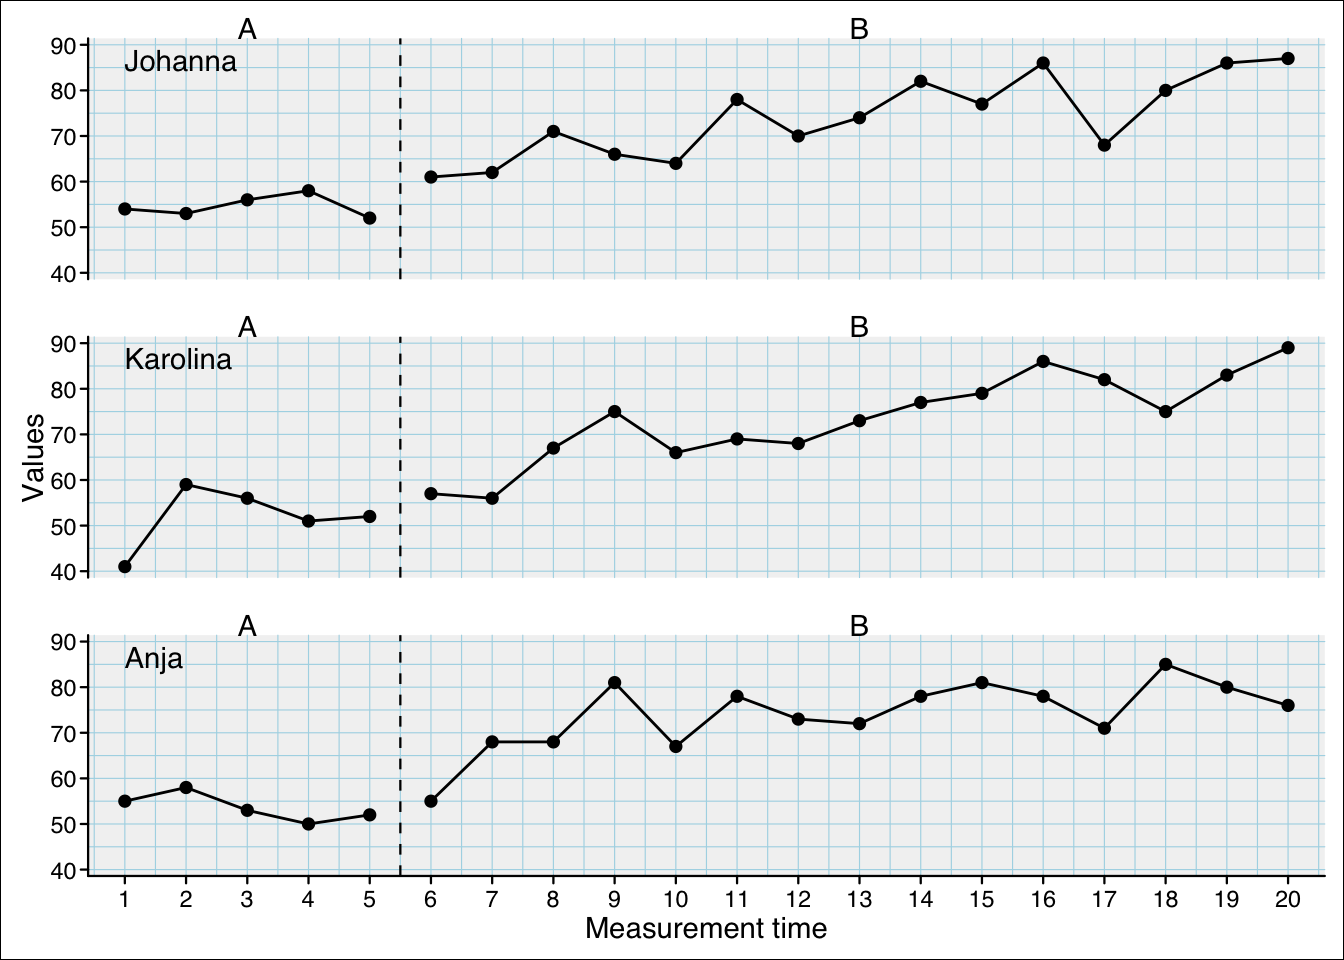
\includegraphics{./ch_scplot_files/figure-pdf/basic2-1.pdf}

}

\end{figure}

\hypertarget{add-datalines}{%
\section{Add datalines}\label{add-datalines}}

\begin{Shaded}
\begin{Highlighting}[]
\FunctionTok{scplot}\NormalTok{(exampleAB\_add) }\SpecialCharTok{\%\textgreater{}\%}
  \FunctionTok{add\_dataline}\NormalTok{(}\StringTok{"depression"}\NormalTok{)}
\end{Highlighting}
\end{Shaded}

\begin{figure}[H]

{\centering 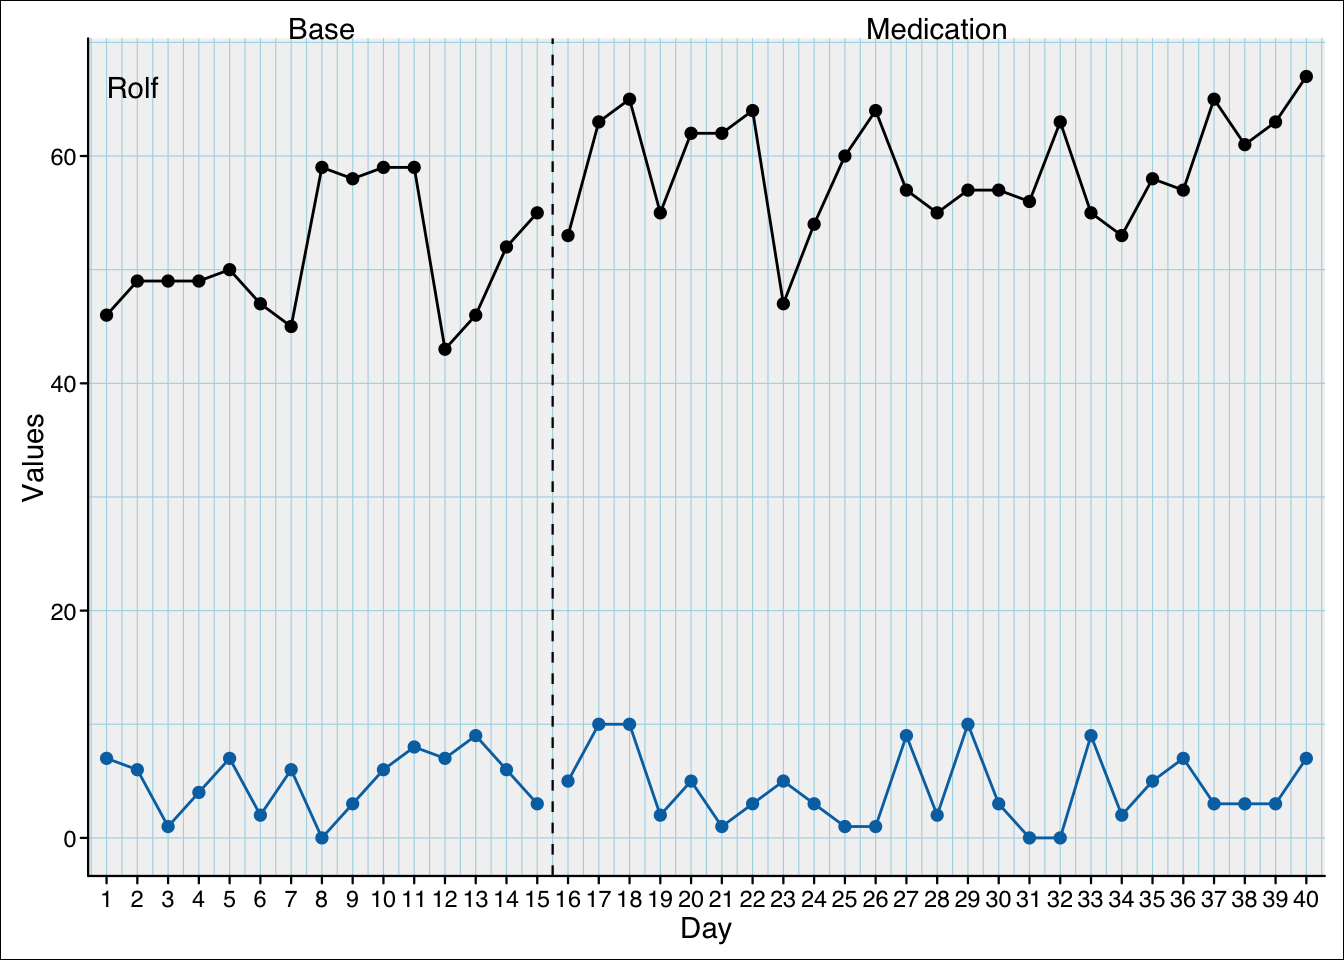
\includegraphics{./ch_scplot_files/figure-pdf/basic3-1.pdf}

}

\end{figure}

\hypertarget{add-statlines}{%
\section{Add statlines}\label{add-statlines}}

\hypertarget{lines-indicating-a-constant-for-each-phase}{%
\subsection{Lines indicating a constant for each
phase}\label{lines-indicating-a-constant-for-each-phase}}

Possible functions: \texttt{mean}, \texttt{min}, \texttt{max},
\texttt{quantile}

\begin{Shaded}
\begin{Highlighting}[]
\FunctionTok{scplot}\NormalTok{(exampleABC) }\SpecialCharTok{\%\textgreater{}\%}
  \FunctionTok{add\_statline}\NormalTok{(}\StringTok{"mean"}\NormalTok{, }\AttributeTok{color =} \StringTok{"darkred"}\NormalTok{) }\SpecialCharTok{\%\textgreater{}\%}
  \FunctionTok{add\_statline}\NormalTok{(}\StringTok{"max"}\NormalTok{, }\AttributeTok{color =} \StringTok{"darkblue"}\NormalTok{, }\AttributeTok{linetype =} \StringTok{"dashed"}\NormalTok{) }\SpecialCharTok{\%\textgreater{}\%}
  \FunctionTok{add\_statline}\NormalTok{(}\StringTok{"min"}\NormalTok{, }\AttributeTok{color =} \StringTok{"brown"}\NormalTok{, }\AttributeTok{linetype =} \StringTok{"dashed"}\NormalTok{)}
\end{Highlighting}
\end{Shaded}

\begin{figure}[H]

{\centering 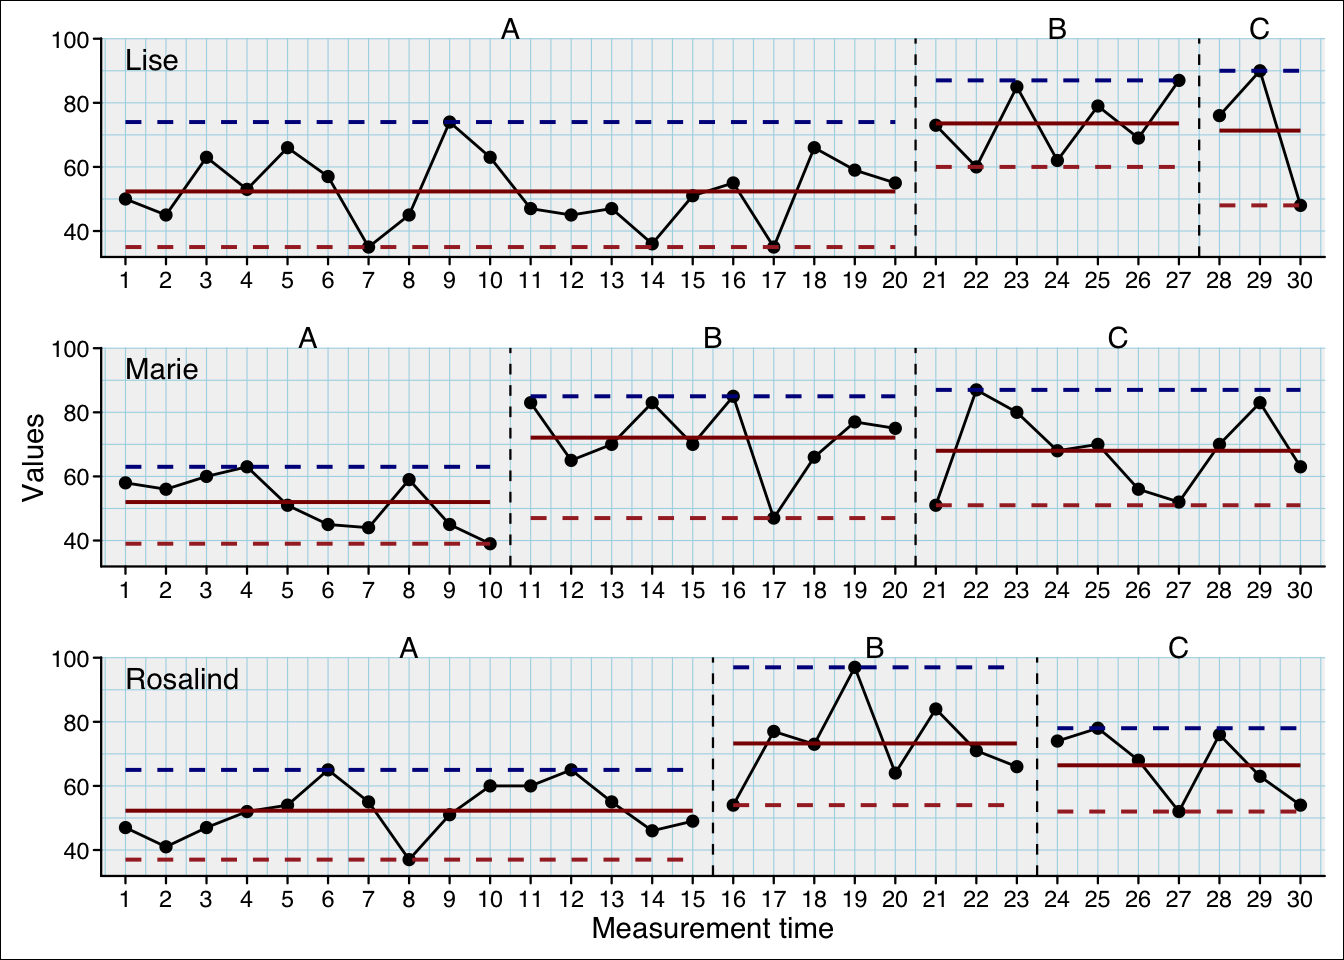
\includegraphics{./ch_scplot_files/figure-pdf/statline1-1.pdf}

}

\end{figure}

\hypertarget{lines-indicating-a-constant-for-a-specific-phase}{%
\subsection{Lines indicating a constant for a specific
phase}\label{lines-indicating-a-constant-for-a-specific-phase}}

Set the \texttt{phase} argument with one or multiple phase-names or
phase-numbers

Possible functions: \texttt{mean}, \texttt{min}, \texttt{max},
\texttt{quantile}

\begin{Shaded}
\begin{Highlighting}[]
\FunctionTok{scplot}\NormalTok{(exampleABC) }\SpecialCharTok{\%\textgreater{}\%}
  \FunctionTok{add\_statline}\NormalTok{(}\StringTok{"mean"}\NormalTok{, }\AttributeTok{phase =} \StringTok{"A"}\NormalTok{, }\AttributeTok{color =} \StringTok{"darkred"}\NormalTok{) }\SpecialCharTok{\%\textgreater{}\%}
  \FunctionTok{add\_statline}\NormalTok{(}\StringTok{"max"}\NormalTok{, }\AttributeTok{phase =} \FunctionTok{c}\NormalTok{(}\StringTok{"B"}\NormalTok{, }\StringTok{"C"}\NormalTok{), }\AttributeTok{color =} \StringTok{"darkblue"}\NormalTok{, }\AttributeTok{linetype =} \StringTok{"dashed"}\NormalTok{) }\SpecialCharTok{\%\textgreater{}\%}
  \FunctionTok{add\_statline}\NormalTok{(}\StringTok{"min"}\NormalTok{, }\AttributeTok{phase =} \FunctionTok{c}\NormalTok{(}\DecValTok{2}\NormalTok{, }\DecValTok{3}\NormalTok{), }\AttributeTok{color =} \StringTok{"orange"}\NormalTok{, }\AttributeTok{linetype =} \StringTok{"dashed"}\NormalTok{)}
\end{Highlighting}
\end{Shaded}

\begin{figure}[H]

{\centering 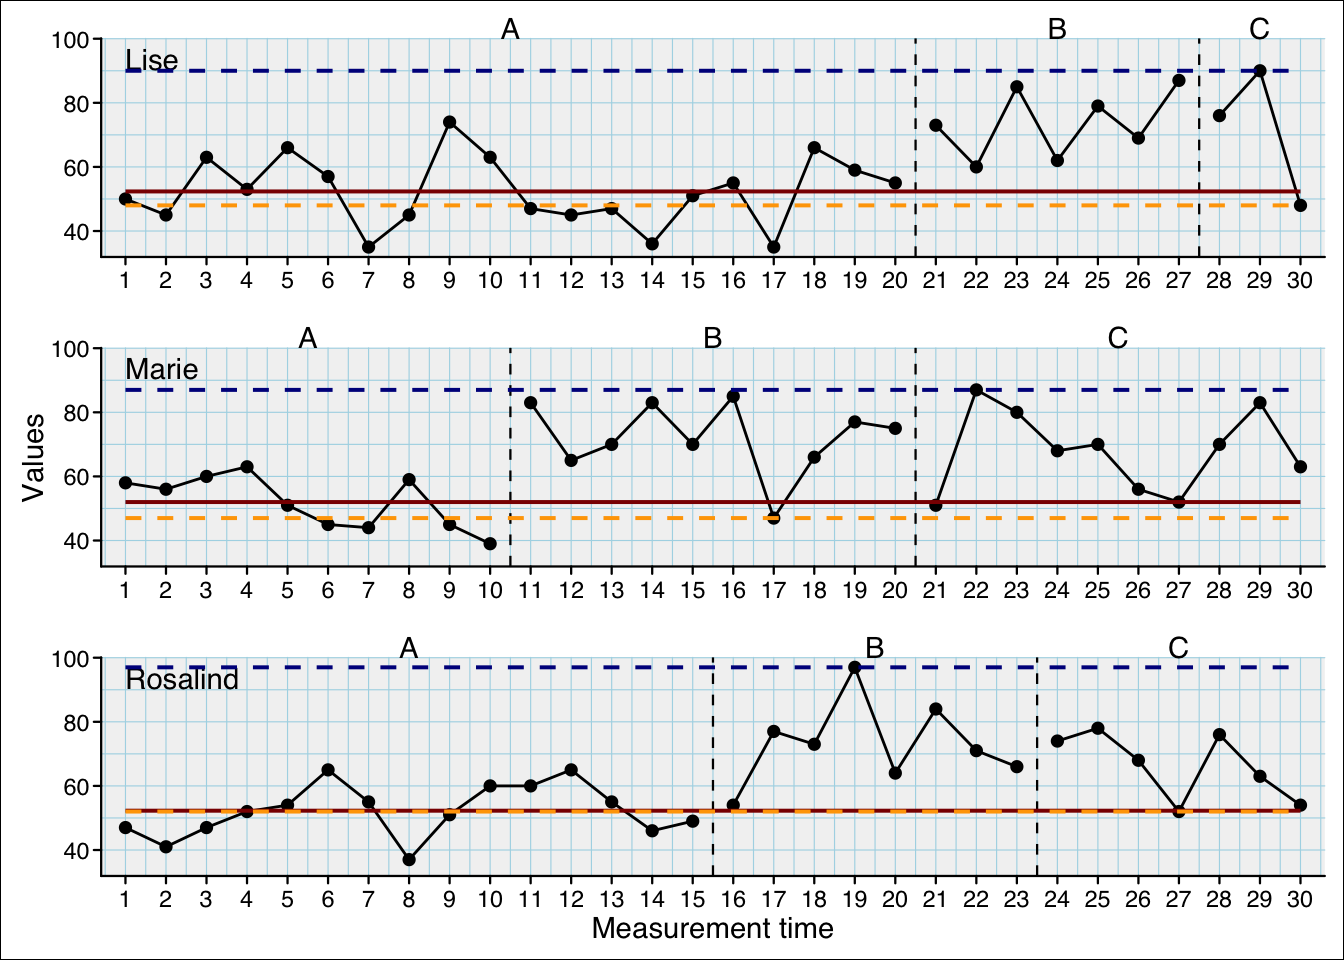
\includegraphics{./ch_scplot_files/figure-pdf/statline2-1.pdf}

}

\end{figure}

\hypertarget{trend-lines}{%
\subsection{Trend-lines}\label{trend-lines}}

\texttt{trend} (separate trend-line for each phase), \texttt{trendA}
(extrapolated trend-line of first phase):

\begin{Shaded}
\begin{Highlighting}[]
\FunctionTok{scplot}\NormalTok{(exampleABC) }\SpecialCharTok{\%\textgreater{}\%}
  \FunctionTok{add\_statline}\NormalTok{(}\StringTok{"trend"}\NormalTok{, }\AttributeTok{color =} \StringTok{"darkred"}\NormalTok{) }\SpecialCharTok{\%\textgreater{}\%}
  \FunctionTok{add\_statline}\NormalTok{(}\StringTok{"trendA"}\NormalTok{, }\AttributeTok{color =} \StringTok{"darkblue"}\NormalTok{, }\AttributeTok{linetype =} \StringTok{"dashed"}\NormalTok{)}
\end{Highlighting}
\end{Shaded}

\begin{figure}[H]

{\centering 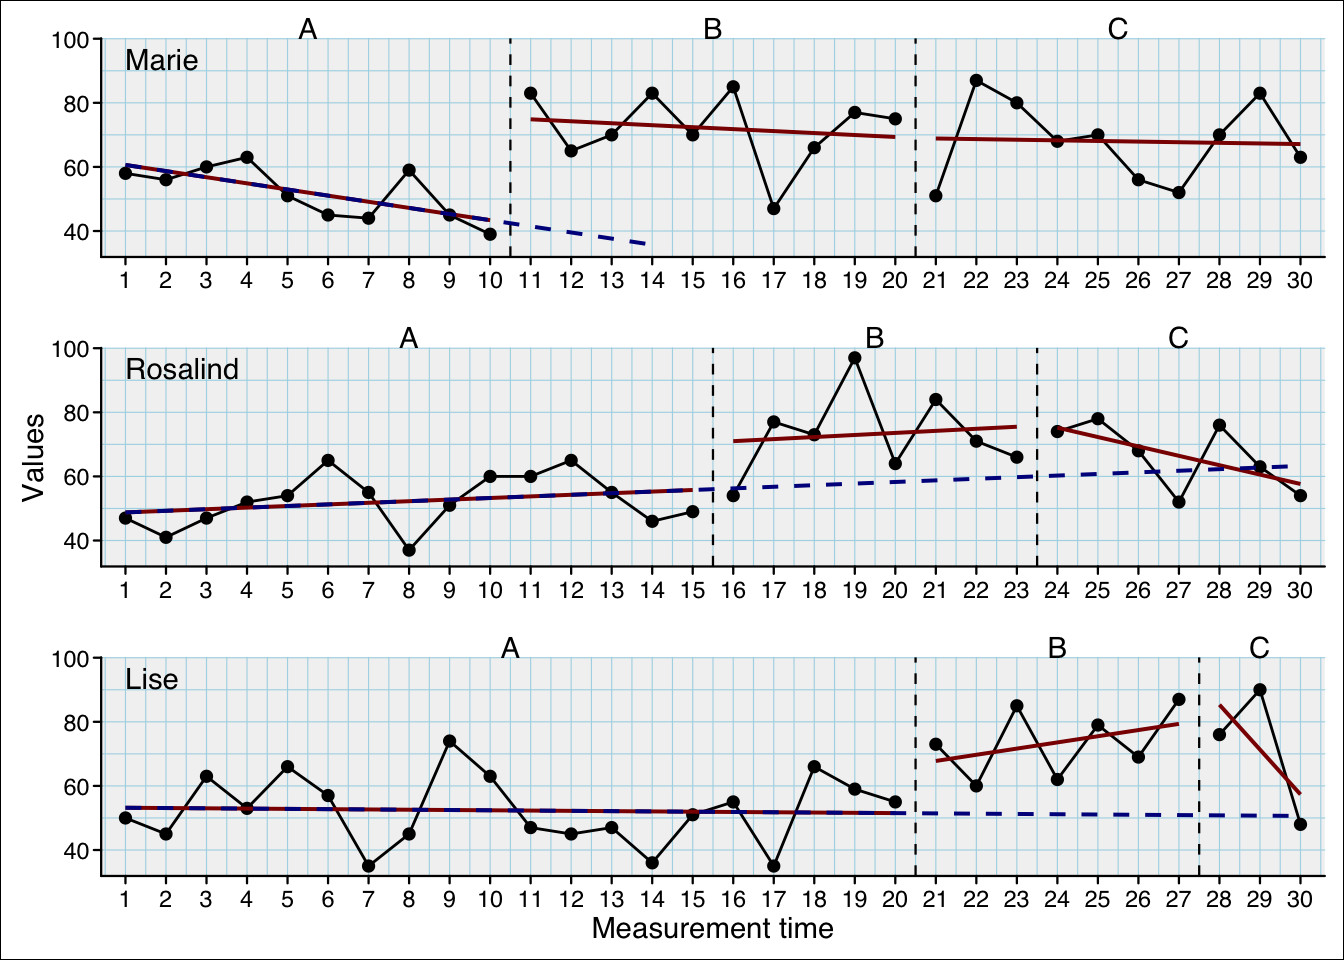
\includegraphics{./ch_scplot_files/figure-pdf/statline3-1.pdf}

}

\end{figure}

\hypertarget{smoothed-curves}{%
\subsection{Smoothed curves}\label{smoothed-curves}}

Possible functions: \texttt{movingMean}, \texttt{movingMedian},
\texttt{loess}, \texttt{lowess}:

\begin{Shaded}
\begin{Highlighting}[]
\FunctionTok{scplot}\NormalTok{(exampleABC) }\SpecialCharTok{\%\textgreater{}\%}
  \FunctionTok{add\_statline}\NormalTok{(}\StringTok{"loess"}\NormalTok{, }\AttributeTok{color =} \StringTok{"darkred"}\NormalTok{) }\SpecialCharTok{\%\textgreater{}\%}
  \FunctionTok{add\_statline}\NormalTok{(}\StringTok{"movingMean"}\NormalTok{, }\AttributeTok{color =} \StringTok{"darkblue"}\NormalTok{)}
\end{Highlighting}
\end{Shaded}

\begin{figure}[H]

{\centering 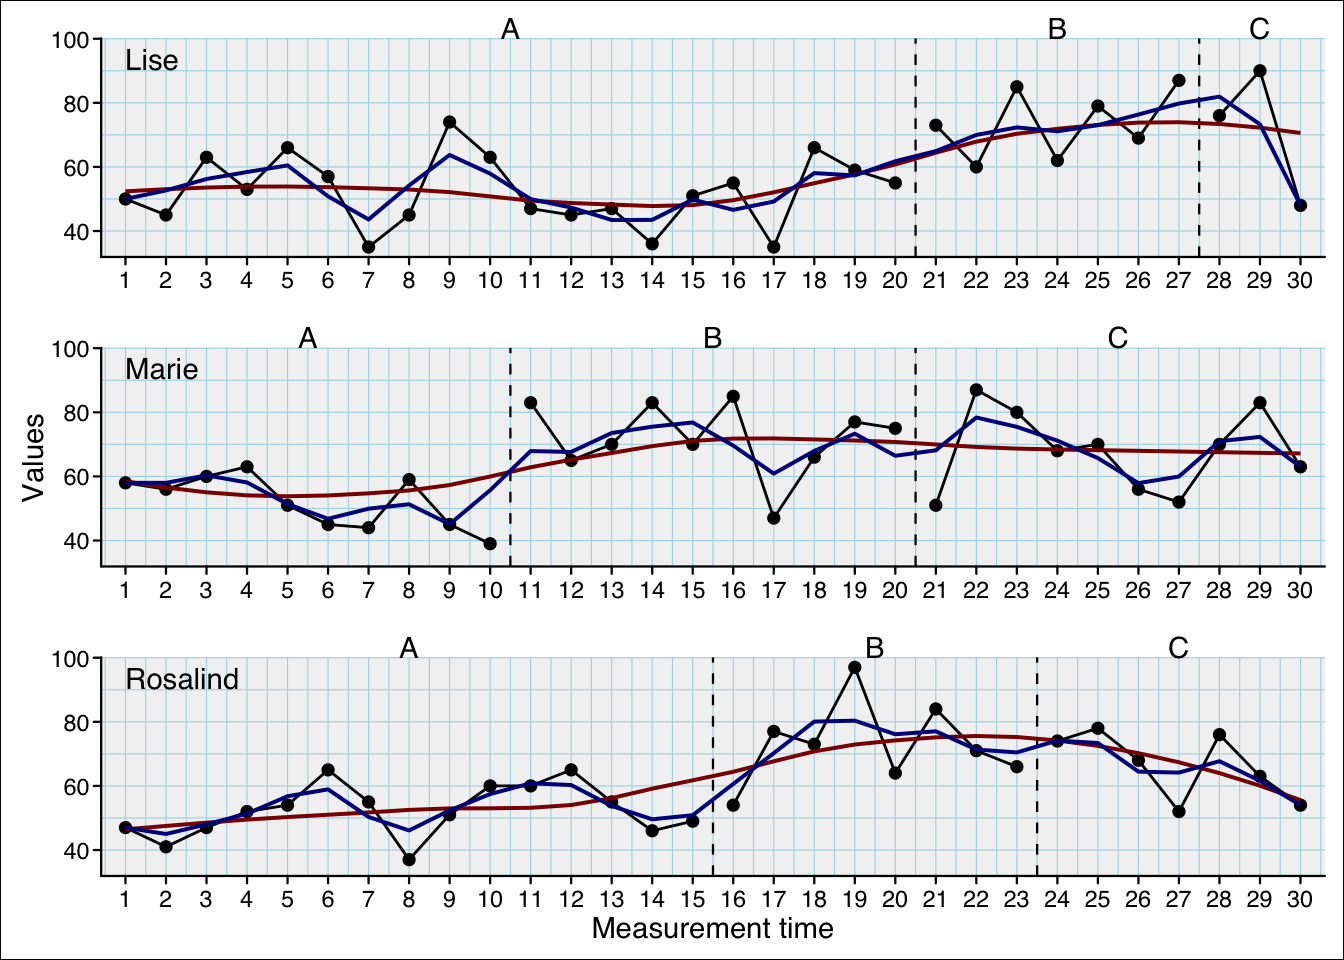
\includegraphics{./ch_scplot_files/figure-pdf/statline4-1.pdf}

}

\end{figure}

\hypertarget{refine-with-addidtional-arguments}{%
\subsection{Refine with addidtional
arguments}\label{refine-with-addidtional-arguments}}

\texttt{mean} : \texttt{trim}\\
\texttt{quantile}: \texttt{probs}\\
\texttt{movingMean}, \texttt{movingMedian}: \texttt{lag}\\
\texttt{loess}: \texttt{span}\\
\texttt{lowess}: \texttt{f}

\begin{Shaded}
\begin{Highlighting}[]
\FunctionTok{scplot}\NormalTok{(exampleABC) }\SpecialCharTok{\%\textgreater{}\%}
  \FunctionTok{add\_statline}\NormalTok{(}\StringTok{"movingMean"}\NormalTok{, }\AttributeTok{lag =} \DecValTok{1}\NormalTok{, }\AttributeTok{color =} \StringTok{"darkblue"}\NormalTok{) }\SpecialCharTok{\%\textgreater{}\%}
  \FunctionTok{add\_statline}\NormalTok{(}\StringTok{"quantile"}\NormalTok{, }\AttributeTok{probs =} \FloatTok{0.75}\NormalTok{, }\AttributeTok{color =} \StringTok{"darkred"}\NormalTok{)}
\end{Highlighting}
\end{Shaded}

\begin{figure}[H]

{\centering 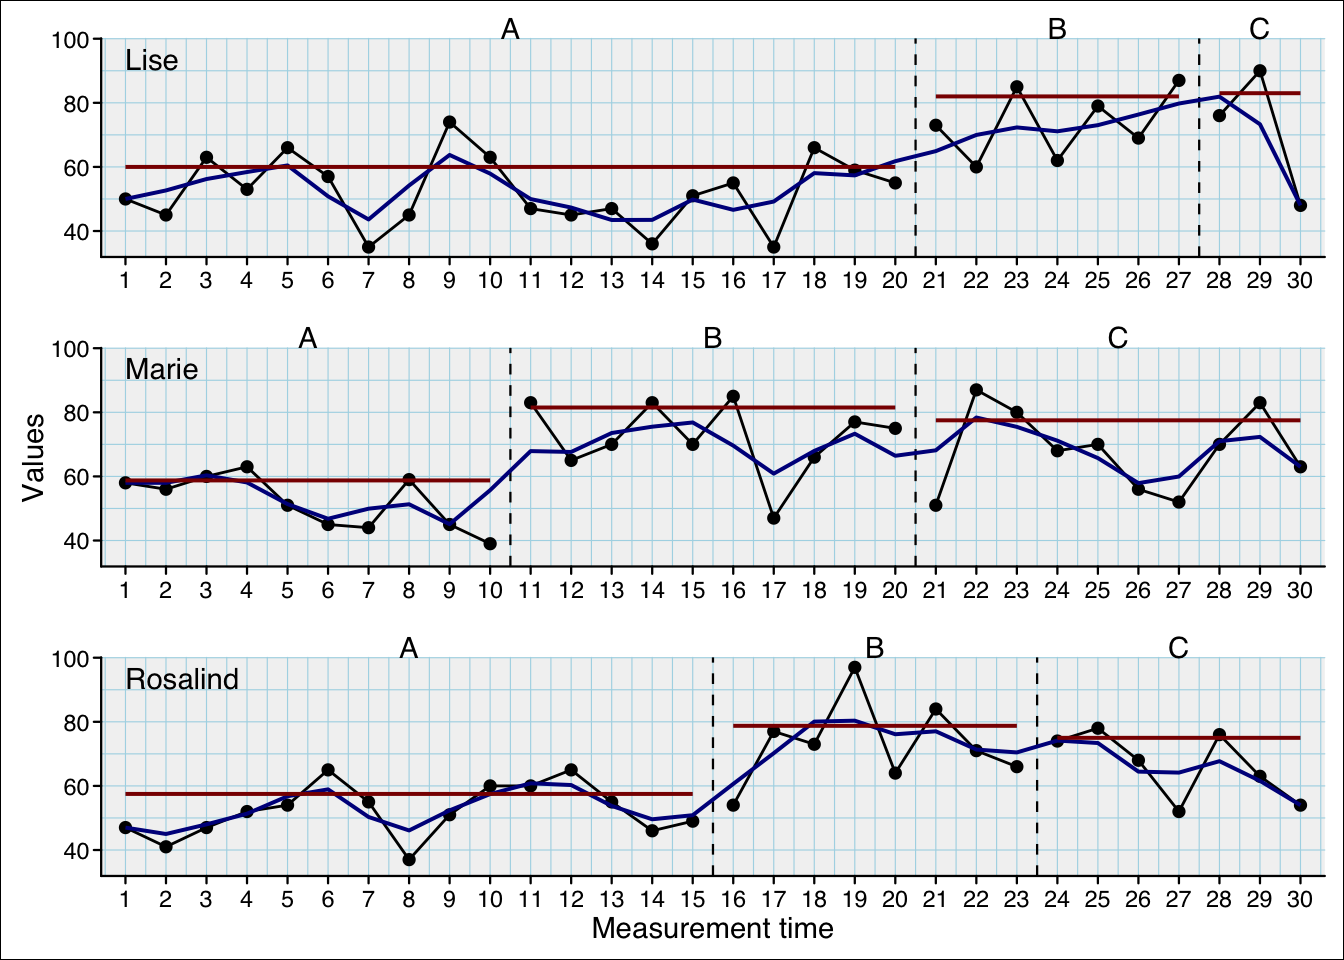
\includegraphics{./ch_scplot_files/figure-pdf/statline5-1.pdf}

}

\end{figure}

\hypertarget{specify-data-line}{%
\subsection{Specify data-line}\label{specify-data-line}}

If you do not specify the \texttt{variable} argument the default first
data-line is addressed.

\begin{Shaded}
\begin{Highlighting}[]
\FunctionTok{scplot}\NormalTok{(exampleAB\_add) }\SpecialCharTok{\%\textgreater{}\%}
  \FunctionTok{add\_dataline}\NormalTok{(}\StringTok{"cigarrets"}\NormalTok{) }\SpecialCharTok{\%\textgreater{}\%}
  \FunctionTok{add\_statline}\NormalTok{(}\StringTok{"mean"}\NormalTok{, }\AttributeTok{variable =} \StringTok{"cigarrets"}\NormalTok{, }\AttributeTok{color =} \StringTok{"darkred"}\NormalTok{) }\SpecialCharTok{\%\textgreater{}\%}
  \FunctionTok{add\_statline}\NormalTok{(}\StringTok{"trend"}\NormalTok{, }\AttributeTok{linetype =} \StringTok{"dashed"}\NormalTok{)}
\end{Highlighting}
\end{Shaded}

\begin{figure}[H]

{\centering 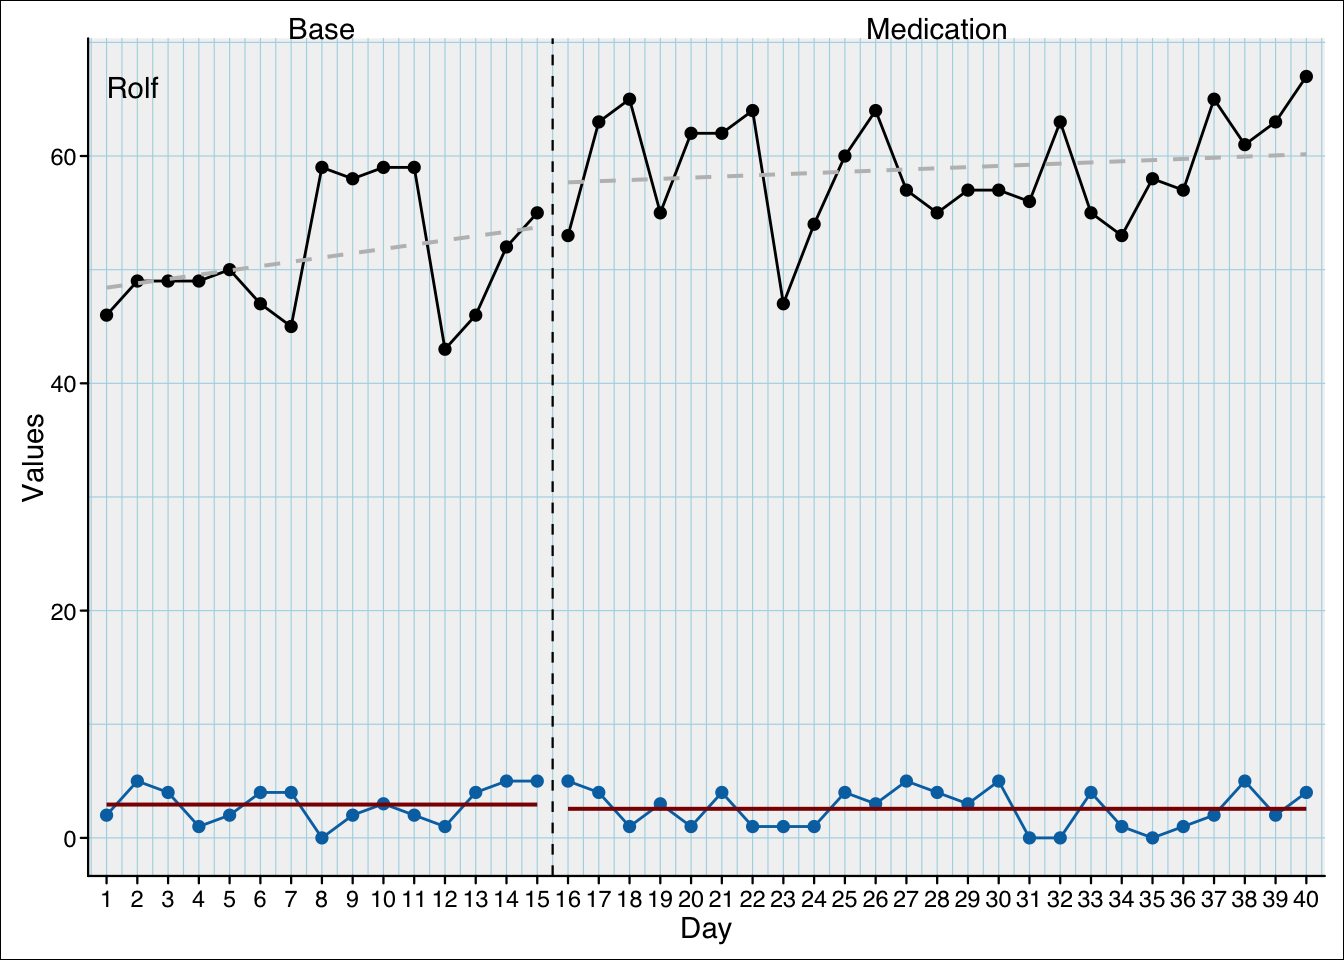
\includegraphics{./ch_scplot_files/figure-pdf/dataline1-1.pdf}

}

\end{figure}

\hypertarget{annotate-and-mark}{%
\section{Annotate and mark}\label{annotate-and-mark}}

\hypertarget{add-marks}{%
\subsection{Add marks}\label{add-marks}}

The positions argument can take a numeric vector:

\begin{Shaded}
\begin{Highlighting}[]
\FunctionTok{scplot}\NormalTok{(exampleABC) }\SpecialCharTok{\%\textgreater{}\%}
  \FunctionTok{add\_marks}\NormalTok{(}\AttributeTok{case =} \DecValTok{1}\NormalTok{, }\AttributeTok{positions =} \FunctionTok{c}\NormalTok{(}\DecValTok{7}\NormalTok{, }\DecValTok{12}\NormalTok{)) }\SpecialCharTok{\%\textgreater{}\%}
  \FunctionTok{add\_marks}\NormalTok{(}\AttributeTok{case =} \DecValTok{3}\NormalTok{, }\AttributeTok{positions =} \FunctionTok{c}\NormalTok{(}\DecValTok{3}\NormalTok{, }\DecValTok{17}\NormalTok{), }\AttributeTok{color =} \StringTok{"blue"}\NormalTok{, }\AttributeTok{size =} \DecValTok{7}\NormalTok{)}
\end{Highlighting}
\end{Shaded}

\begin{figure}[H]

{\centering 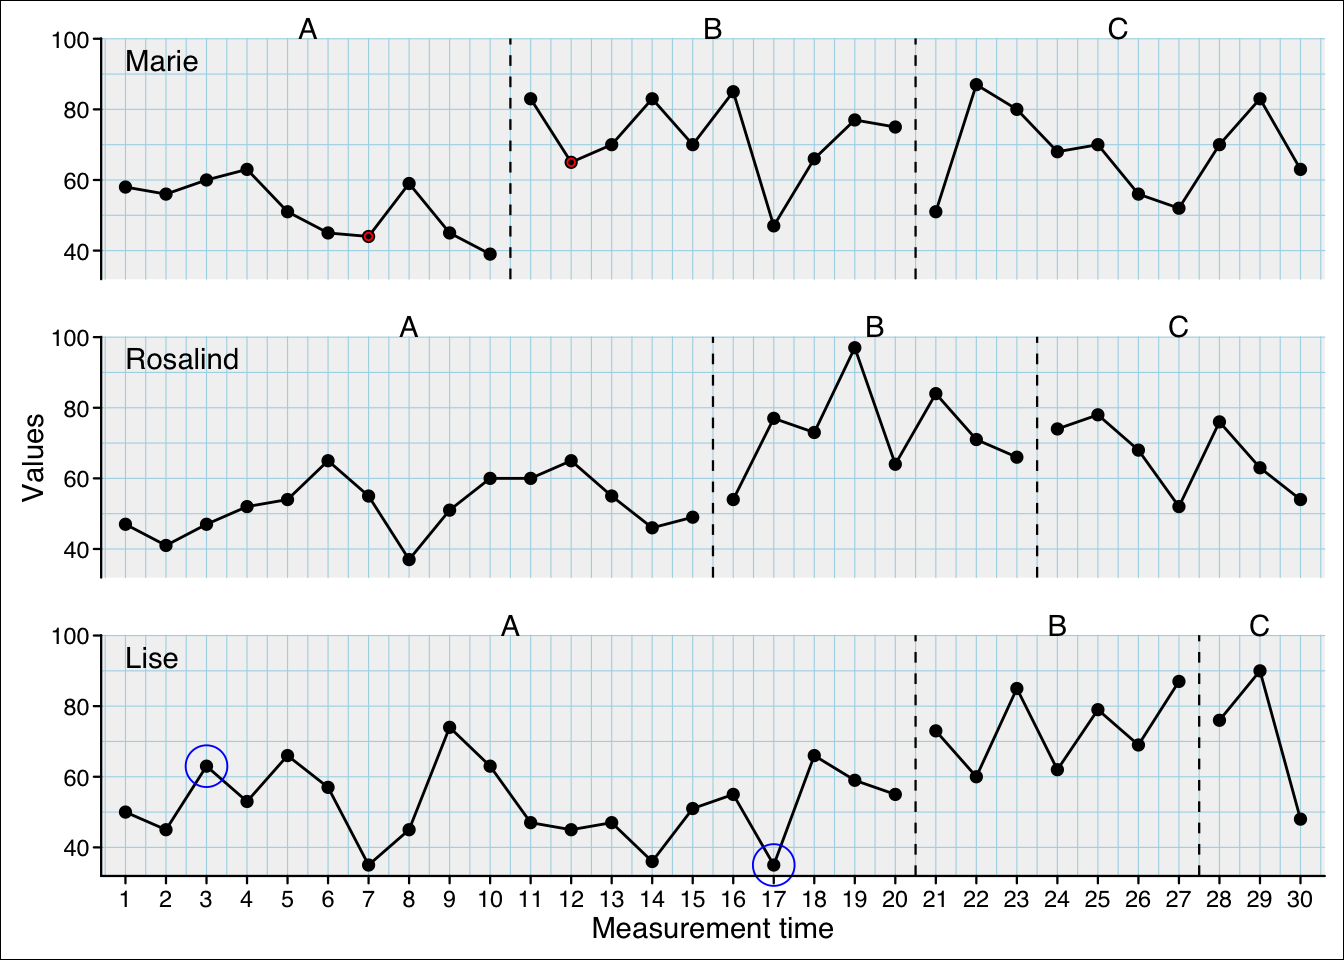
\includegraphics{./ch_scplot_files/figure-pdf/marks1-1.pdf}

}

\end{figure}

The positions argument can also be a string containing a logical
expression. This will be evaluated and the respective positions will be
marked.

\begin{Shaded}
\begin{Highlighting}[]
\FunctionTok{scplot}\NormalTok{(exampleABC) }\SpecialCharTok{\%\textgreater{}\%}
  \FunctionTok{add\_marks}\NormalTok{(}\AttributeTok{case =} \DecValTok{1}\NormalTok{, }\AttributeTok{positions =} \StringTok{"mt \textgreater{} 15"}\NormalTok{) }\SpecialCharTok{\%\textgreater{}\%}
  \FunctionTok{add\_marks}\NormalTok{(}\AttributeTok{case =} \DecValTok{2}\NormalTok{, }\AttributeTok{positions =} \StringTok{\textquotesingle{}phase == "B"\textquotesingle{}}\NormalTok{, }\AttributeTok{color =} \StringTok{"green"}\NormalTok{, }\AttributeTok{size =} \DecValTok{5}\NormalTok{) }\SpecialCharTok{\%\textgreater{}\%}
  \FunctionTok{add\_marks}\NormalTok{(}\AttributeTok{case =} \DecValTok{3}\NormalTok{, }\AttributeTok{positions =} \StringTok{"values \textgreater{} quantile(values, probs = 0.80)"}\NormalTok{, }\AttributeTok{color =} \StringTok{"blue"}\NormalTok{, }\AttributeTok{size =} \DecValTok{7}\NormalTok{) }\SpecialCharTok{\%\textgreater{}\%}
  \FunctionTok{add\_marks}\NormalTok{(}\AttributeTok{case =} \StringTok{"all"}\NormalTok{, }\AttributeTok{positions =} \StringTok{"values \textless{} quantile(values, probs = 0.20)"}\NormalTok{, }\AttributeTok{color =} \StringTok{"yellow"}\NormalTok{, }\AttributeTok{size =} \DecValTok{7}\NormalTok{) }\SpecialCharTok{\%\textgreater{}\%}
  \FunctionTok{add\_caption}\NormalTok{(}\StringTok{"Note.}
\StringTok{red: mt \textgreater{} 15 in case 1; }
\StringTok{green: phase \textquotesingle{}B\textquotesingle{} in case 2; }
\StringTok{blue: values \textgreater{} 80\% quantile of case 3; }
\StringTok{yellow: values \textless{} 20\% quantile of all cases"}\NormalTok{)}
\end{Highlighting}
\end{Shaded}

\begin{figure}[H]

{\centering 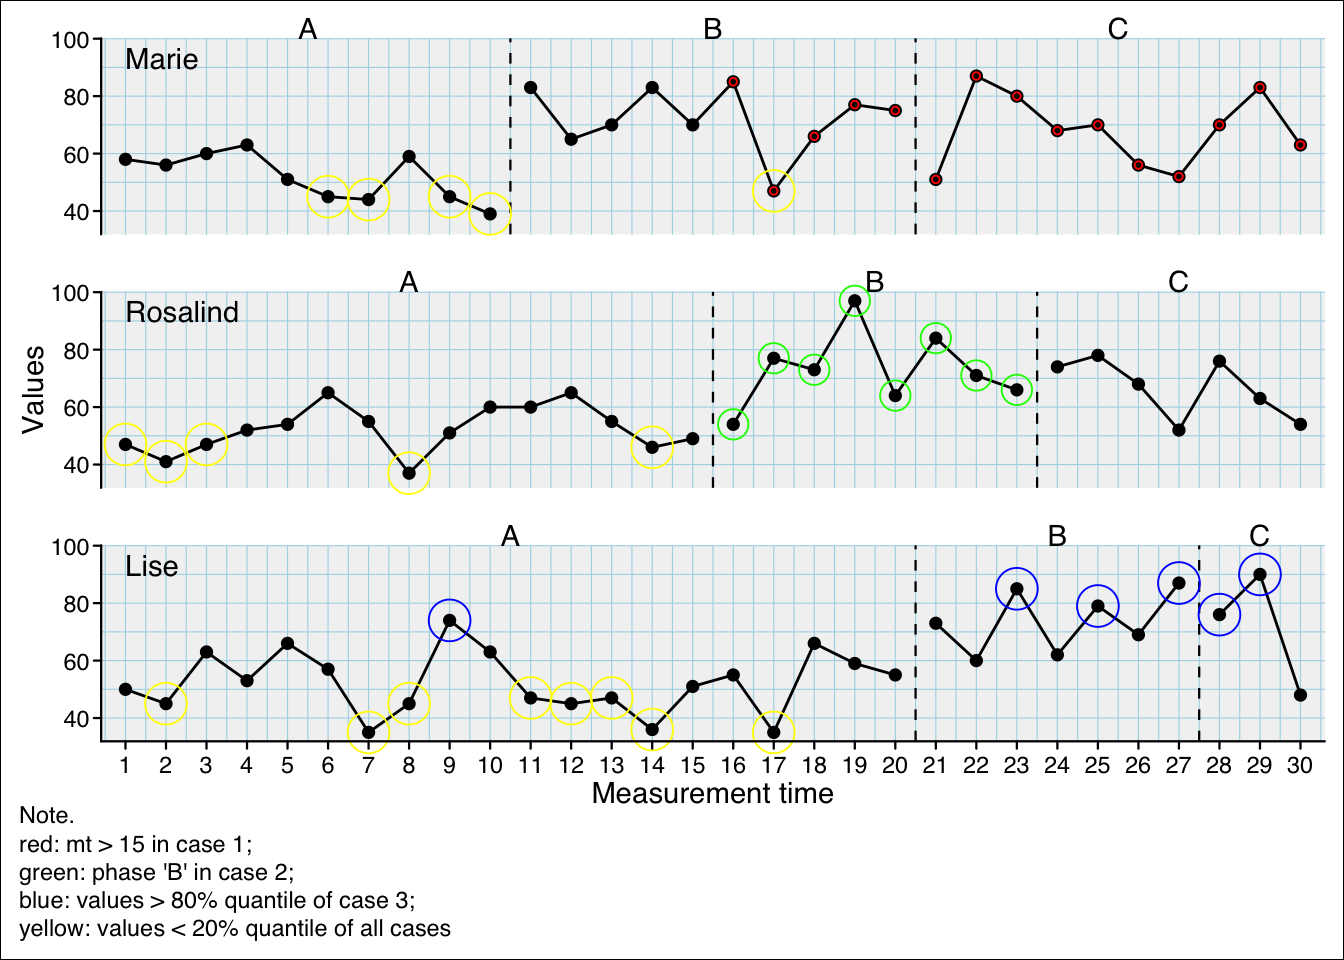
\includegraphics{./ch_scplot_files/figure-pdf/marks2-1.pdf}

}

\end{figure}

And the positions argument can take the results from a scan outlier
analyses and mark the positions of the outliers of each case:

\begin{Shaded}
\begin{Highlighting}[]
\FunctionTok{scplot}\NormalTok{(exampleABC\_outlier) }\SpecialCharTok{\%\textgreater{}\%} 
  \FunctionTok{add\_marks}\NormalTok{(}\AttributeTok{positions =} \FunctionTok{outlier}\NormalTok{(exampleABC\_outlier), }\AttributeTok{size =} \DecValTok{3}\NormalTok{)}
\end{Highlighting}
\end{Shaded}

\begin{figure}[H]

{\centering 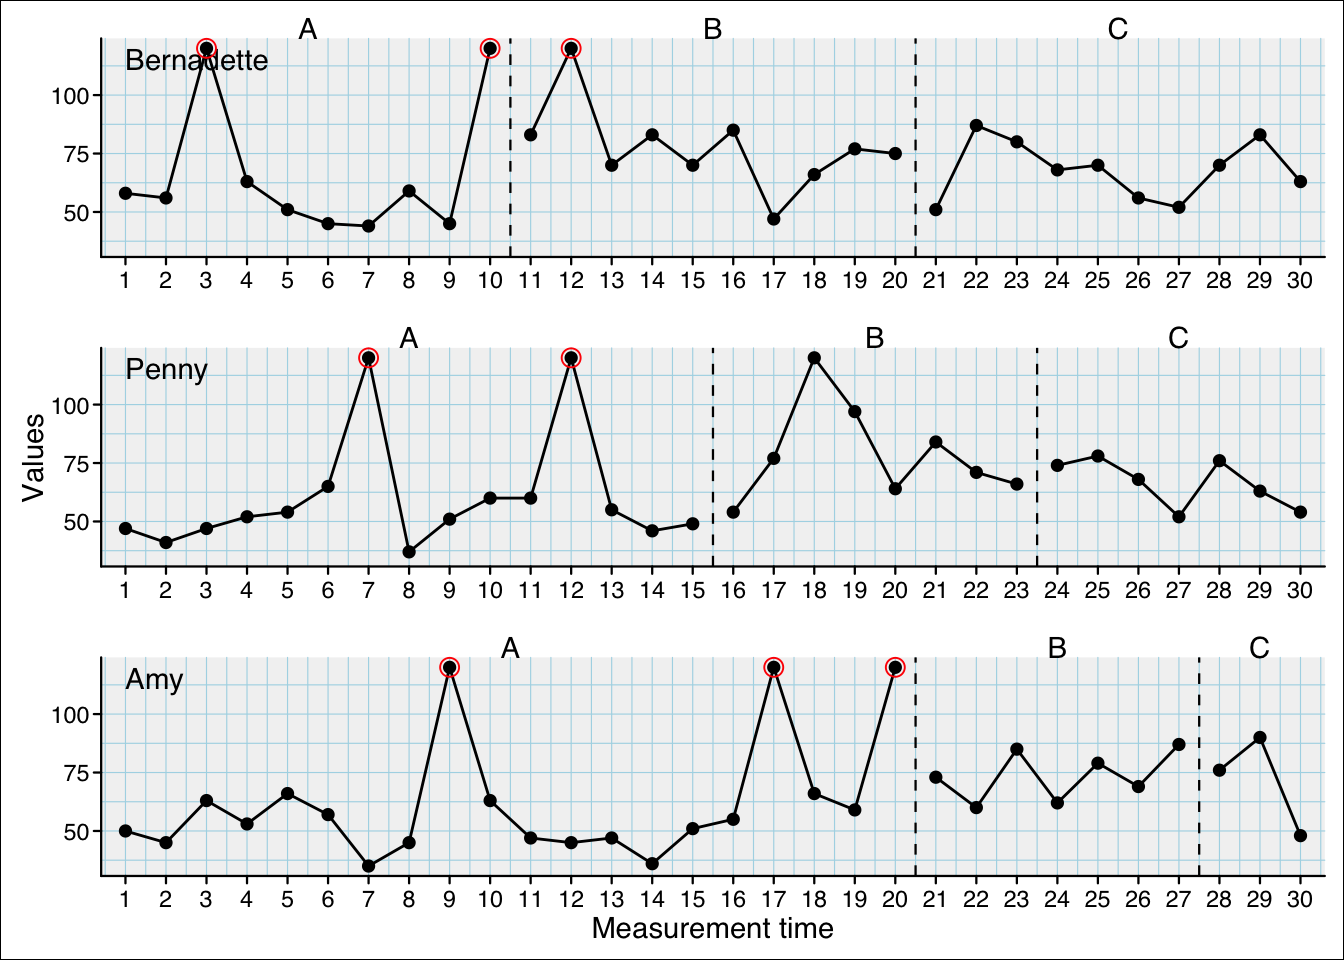
\includegraphics{./ch_scplot_files/figure-pdf/marks3-1.pdf}

}

\end{figure}

\hypertarget{add-text}{%
\subsection{Add text}\label{add-text}}

\begin{Shaded}
\begin{Highlighting}[]
\FunctionTok{scplot}\NormalTok{(exampleABC) }\SpecialCharTok{\%\textgreater{}\%}
  \FunctionTok{add\_text}\NormalTok{(}\StringTok{"Here!"}\NormalTok{, }\AttributeTok{case =} \DecValTok{2}\NormalTok{, }\AttributeTok{x =} \DecValTok{10}\NormalTok{, }\AttributeTok{y =} \DecValTok{80}\NormalTok{, }\AttributeTok{color =} \StringTok{"red"}\NormalTok{)}
\end{Highlighting}
\end{Shaded}

\begin{figure}[H]

{\centering 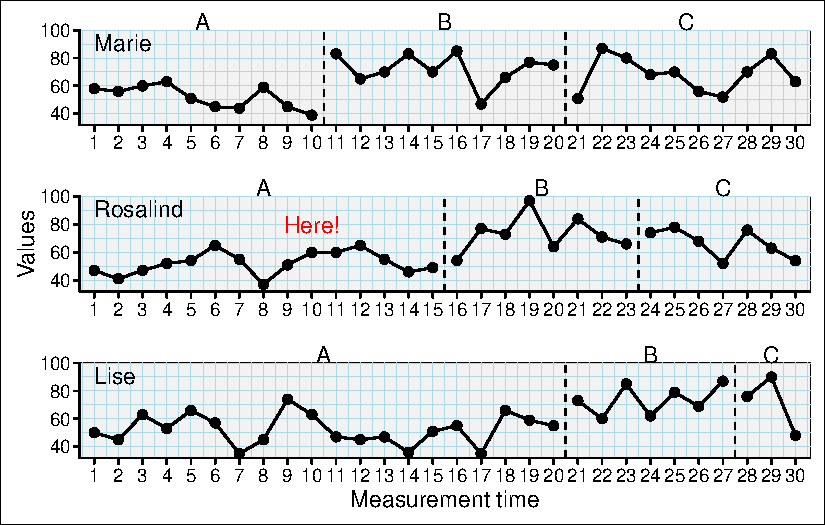
\includegraphics{./ch_scplot_files/figure-pdf/text1-1.pdf}

}

\end{figure}

\hypertarget{add-arrow}{%
\subsection{Add arrow}\label{add-arrow}}

\begin{Shaded}
\begin{Highlighting}[]
\FunctionTok{scplot}\NormalTok{(exampleABC) }\SpecialCharTok{\%\textgreater{}\%}
  \FunctionTok{add\_arrow}\NormalTok{(}\AttributeTok{case =} \DecValTok{1}\NormalTok{, }\AttributeTok{x0 =} \DecValTok{6}\NormalTok{, }\AttributeTok{y0 =} \DecValTok{90}\NormalTok{, }\AttributeTok{x1 =} \DecValTok{3}\NormalTok{, }\AttributeTok{y1 =} \DecValTok{63}\NormalTok{) }\SpecialCharTok{\%\textgreater{}\%}
  \FunctionTok{add\_text}\NormalTok{(}\StringTok{"Problem"}\NormalTok{, }\AttributeTok{case =} \DecValTok{1}\NormalTok{, }\AttributeTok{x =} \DecValTok{6}\NormalTok{, }\AttributeTok{y =} \DecValTok{94}\NormalTok{, }\AttributeTok{color =} \StringTok{"red"}\NormalTok{, }\AttributeTok{size =} \DecValTok{1}\NormalTok{, }\AttributeTok{hjust =} \DecValTok{0}\NormalTok{ ) }
\end{Highlighting}
\end{Shaded}

\begin{figure}[H]

{\centering 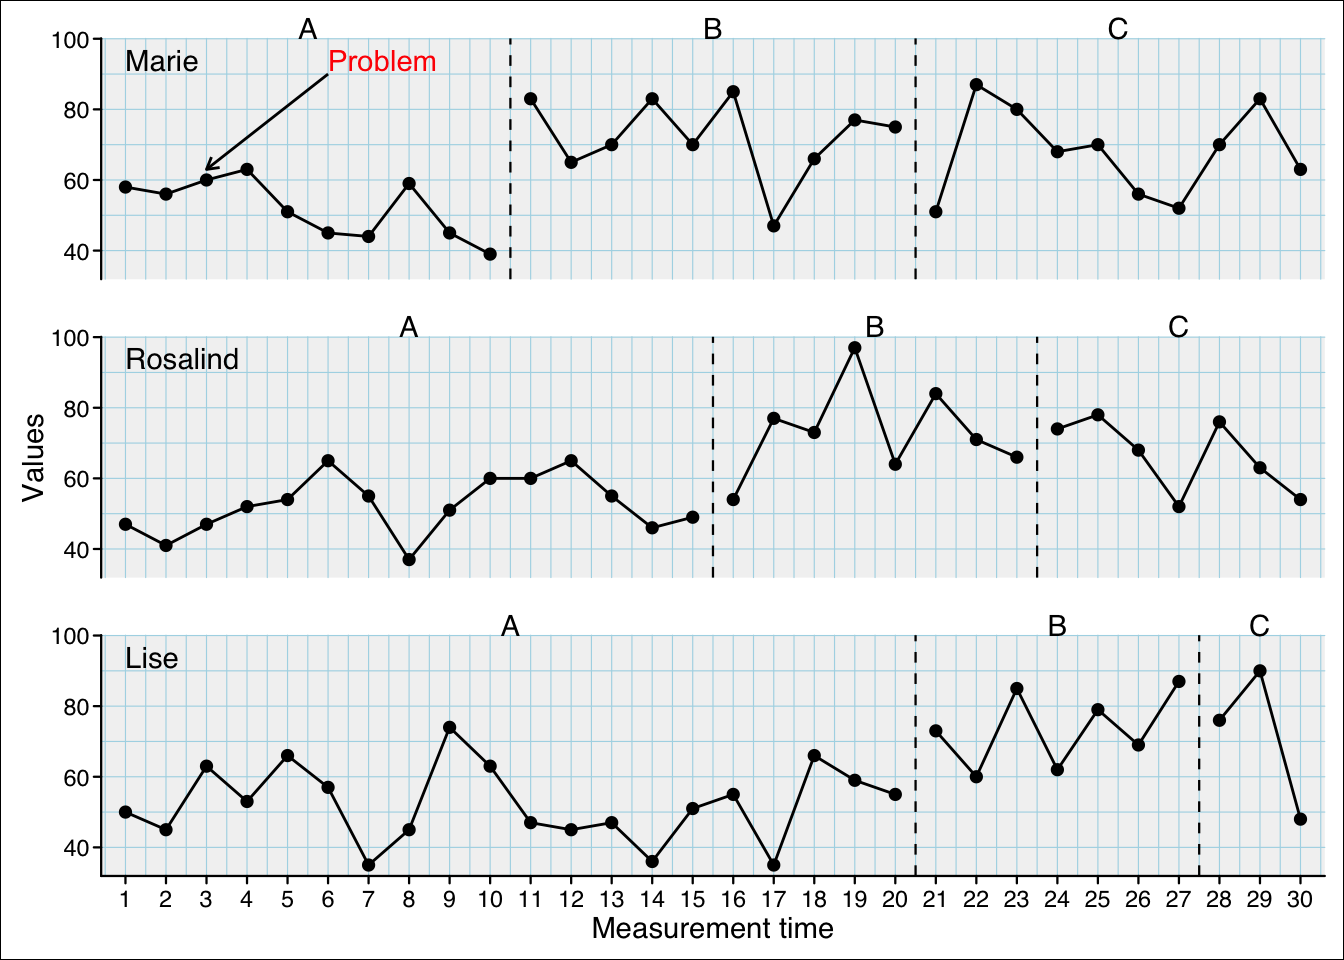
\includegraphics{./ch_scplot_files/figure-pdf/arrow1-1.pdf}

}

\end{figure}

\hypertarget{change-appearance-of-basic-plot-elements}{%
\section{Change appearance of basic plot
elements}\label{change-appearance-of-basic-plot-elements}}

\hypertarget{data-line}{%
\subsection{Data line}\label{data-line}}

\begin{Shaded}
\begin{Highlighting}[]
\FunctionTok{scplot}\NormalTok{(exampleABC) }\SpecialCharTok{\%\textgreater{}\%}
  \FunctionTok{set\_dataline}\NormalTok{(}\AttributeTok{colour =} \StringTok{"blue"}\NormalTok{, }\AttributeTok{size =} \DecValTok{1}\NormalTok{, }\AttributeTok{linetype =} \StringTok{"dotted"}\NormalTok{, }
               \AttributeTok{point =} \FunctionTok{list}\NormalTok{(}\AttributeTok{colour =} \StringTok{"red"}\NormalTok{, }\AttributeTok{size =} \DecValTok{1}\NormalTok{, }\AttributeTok{shape =} \DecValTok{2}\NormalTok{) )}
\end{Highlighting}
\end{Shaded}

\begin{figure}[H]

{\centering 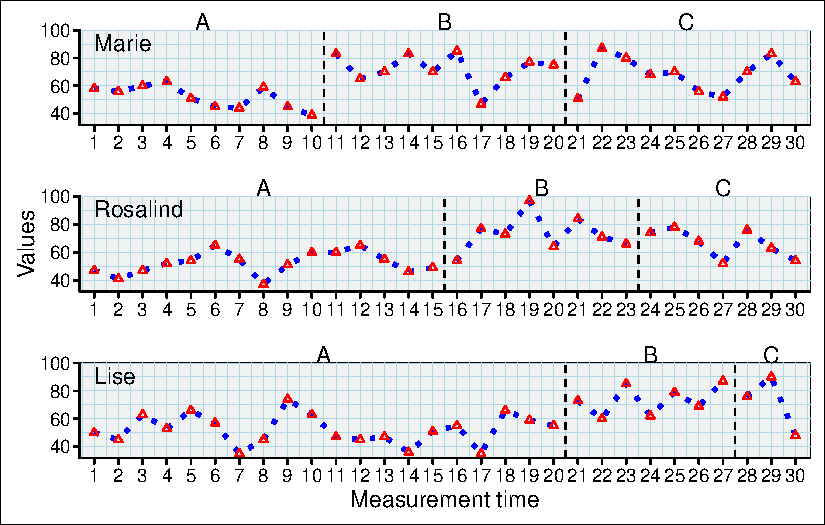
\includegraphics{./ch_scplot_files/figure-pdf/line1-1.pdf}

}

\end{figure}

\begin{Shaded}
\begin{Highlighting}[]
\CommentTok{\# Equivalent\_}
\CommentTok{\# scplot(exampleABC) \%\textgreater{}\%}
\CommentTok{\#   set\_dataline(line = list(colour = "blue", size = 1, linetype = "dotted"), }
\CommentTok{\#                point = list(colour = "red", size = 1, shape = 2)) }
\end{Highlighting}
\end{Shaded}

\hypertarget{background}{%
\subsection{Background}\label{background}}

\begin{Shaded}
\begin{Highlighting}[]
\FunctionTok{scplot}\NormalTok{(exampleABC) }\SpecialCharTok{\%\textgreater{}\%}
  \FunctionTok{set\_background}\NormalTok{(}\AttributeTok{fill =} \StringTok{"grey90"}\NormalTok{, }\AttributeTok{color =} \StringTok{"black"}\NormalTok{, }\AttributeTok{size =} \DecValTok{2}\NormalTok{)}
\end{Highlighting}
\end{Shaded}

\begin{figure}[H]

{\centering 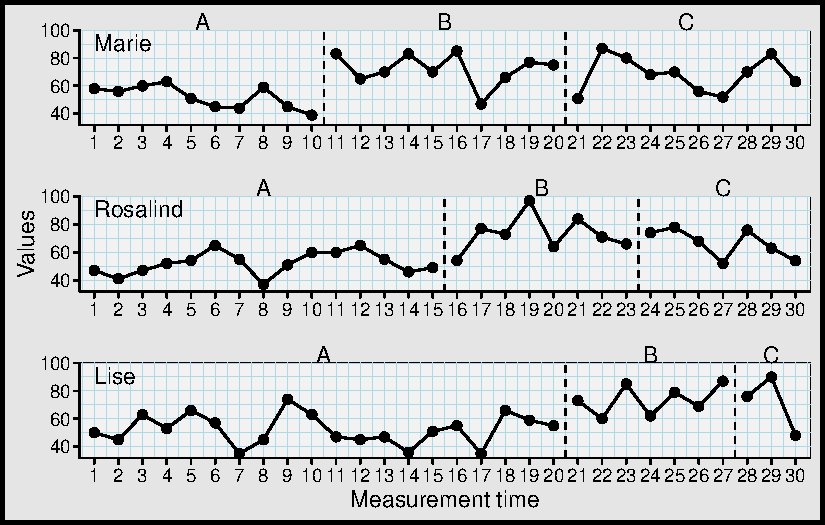
\includegraphics{./ch_scplot_files/figure-pdf/background1-1.pdf}

}

\end{figure}

\hypertarget{panel}{%
\subsection{Panel}\label{panel}}

\begin{Shaded}
\begin{Highlighting}[]
\FunctionTok{scplot}\NormalTok{(exampleABC) }\SpecialCharTok{\%\textgreater{}\%}
  \FunctionTok{set\_panel}\NormalTok{(}\AttributeTok{fill =} \StringTok{"tan1"}\NormalTok{, }\AttributeTok{color =} \StringTok{"palevioletred"}\NormalTok{, }\AttributeTok{size =} \DecValTok{2}\NormalTok{)}
\end{Highlighting}
\end{Shaded}

\begin{figure}[H]

{\centering 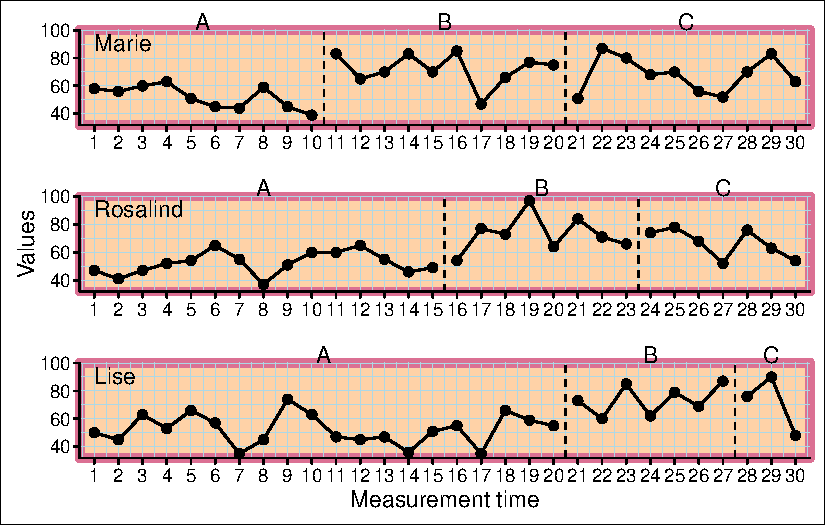
\includegraphics{./ch_scplot_files/figure-pdf/pannel1-1.pdf}

}

\end{figure}

\hypertarget{a-different-panel-color-for-each-phase}{%
\subsection{A different panel color for each
phase}\label{a-different-panel-color-for-each-phase}}

Note: The colors are 50\% transparent. So they might appear different.

\begin{Shaded}
\begin{Highlighting}[]
\FunctionTok{scplot}\NormalTok{(exampleABC) }\SpecialCharTok{\%\textgreater{}\%}
  \FunctionTok{set\_panel}\NormalTok{(}\AttributeTok{fill =} \FunctionTok{c}\NormalTok{(}\StringTok{"grey80"}\NormalTok{, }\StringTok{"white"}\NormalTok{, }\StringTok{"blue4"}\NormalTok{))}
\end{Highlighting}
\end{Shaded}

\begin{figure}[H]

{\centering 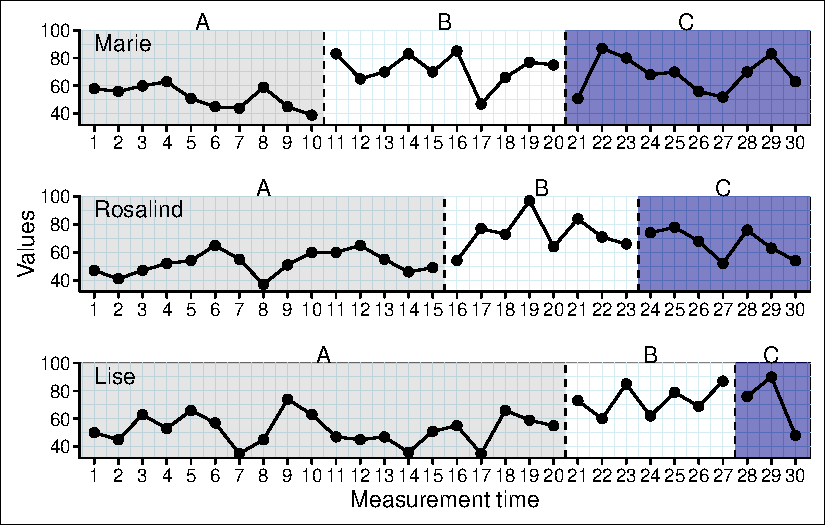
\includegraphics{./ch_scplot_files/figure-pdf/pannel2-1.pdf}

}

\end{figure}

\hypertarget{themes}{%
\section{Themes}\label{themes}}

Themes are complete styles that define various elements of a plot.

Function \texttt{add\_theme("theme\_name")}

Possible themes:

\texttt{basic}, \texttt{grid}, \texttt{default}, \texttt{small},
\texttt{tiny}, \texttt{big}, \texttt{minimal}, \texttt{dark},
\texttt{sienna}, \texttt{phase\_color}, \texttt{phase\_shade},
\texttt{grid2}

\hypertarget{the-default-theme}{%
\subsection{The `default' theme}\label{the-default-theme}}

\begin{Shaded}
\begin{Highlighting}[]
\FunctionTok{scplot}\NormalTok{(exampleABC)}
\end{Highlighting}
\end{Shaded}

\begin{figure}[H]

{\centering 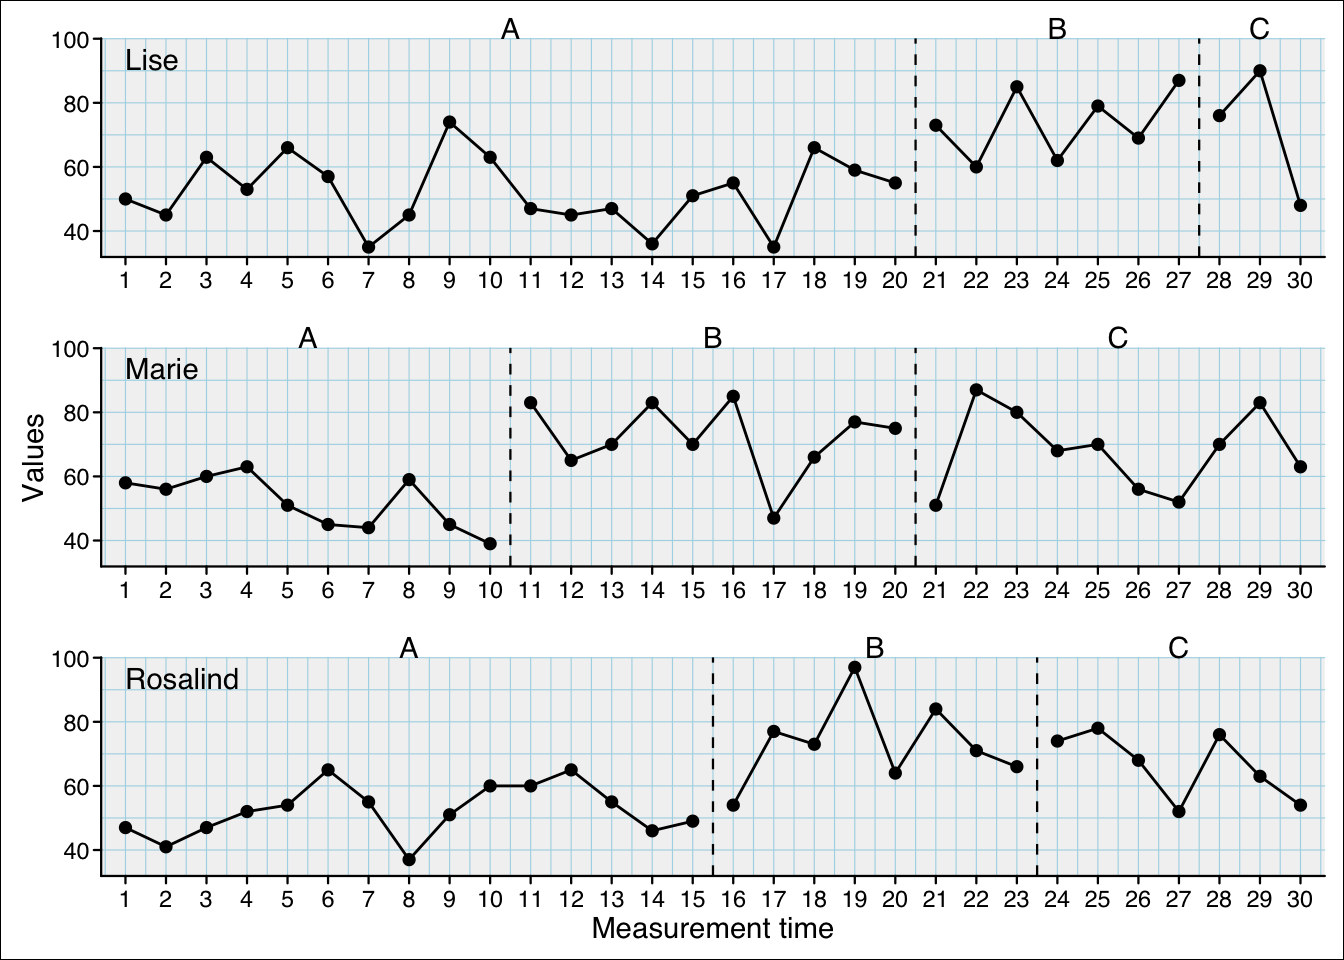
\includegraphics{./ch_scplot_files/figure-pdf/theme2-1.pdf}

}

\end{figure}

\hypertarget{theme-basic}{%
\subsection{Theme `basic'}\label{theme-basic}}

\begin{Shaded}
\begin{Highlighting}[]
\FunctionTok{scplot}\NormalTok{(exampleABC) }\SpecialCharTok{\%\textgreater{}\%}
  \FunctionTok{add\_theme}\NormalTok{(}\StringTok{"basic"}\NormalTok{)}
\end{Highlighting}
\end{Shaded}

\begin{figure}[H]

{\centering 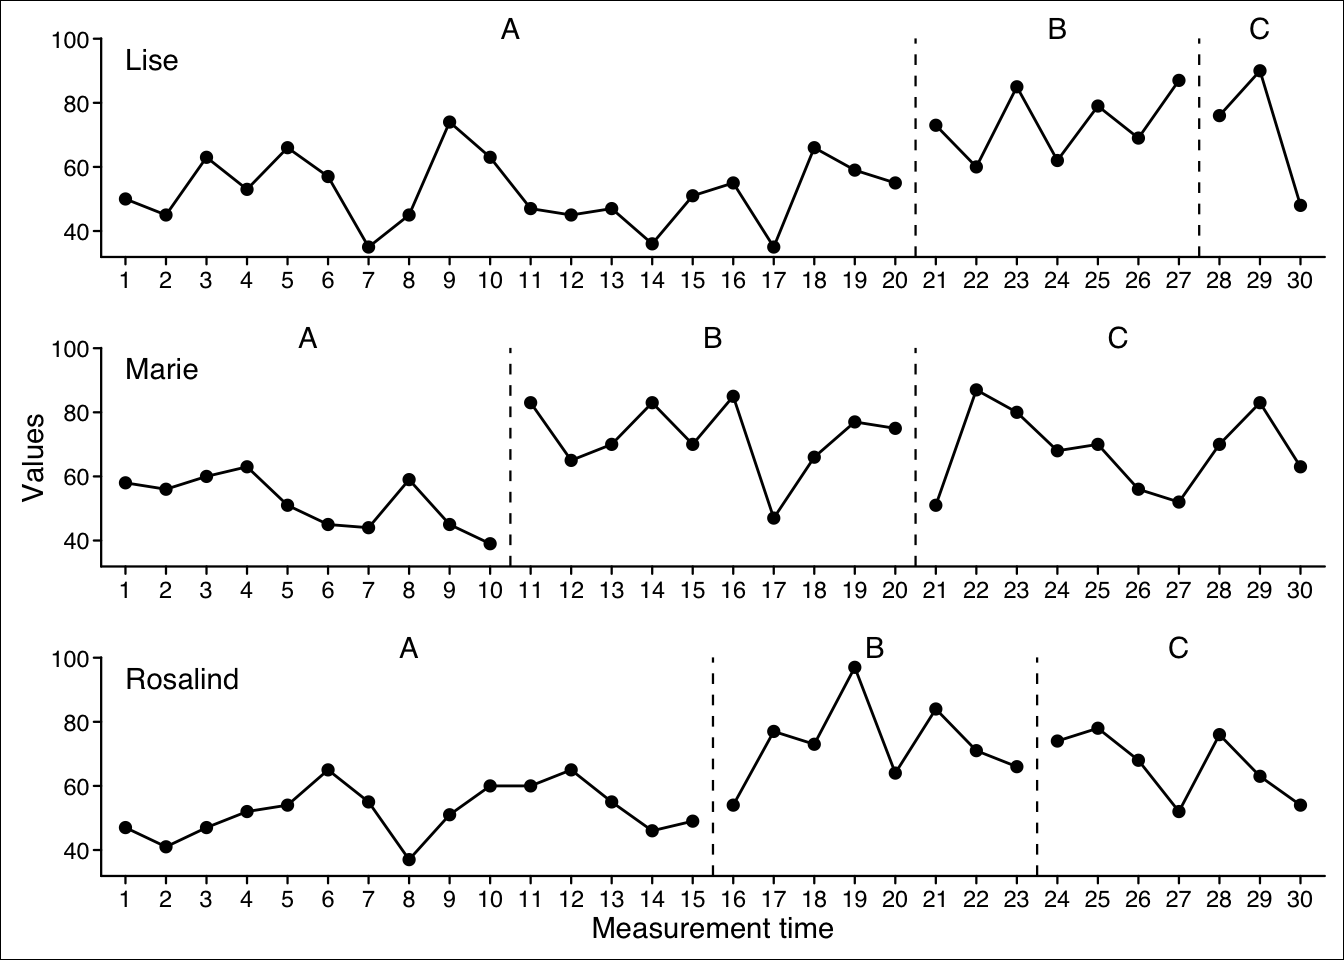
\includegraphics{./ch_scplot_files/figure-pdf/theme3-1.pdf}

}

\end{figure}

\hypertarget{theme-minimal}{%
\subsection{Theme `minimal'}\label{theme-minimal}}

\begin{Shaded}
\begin{Highlighting}[]
\FunctionTok{scplot}\NormalTok{(exampleABC) }\SpecialCharTok{\%\textgreater{}\%}
  \FunctionTok{add\_theme}\NormalTok{(}\StringTok{"minimal"}\NormalTok{)}
\end{Highlighting}
\end{Shaded}

\begin{figure}[H]

{\centering 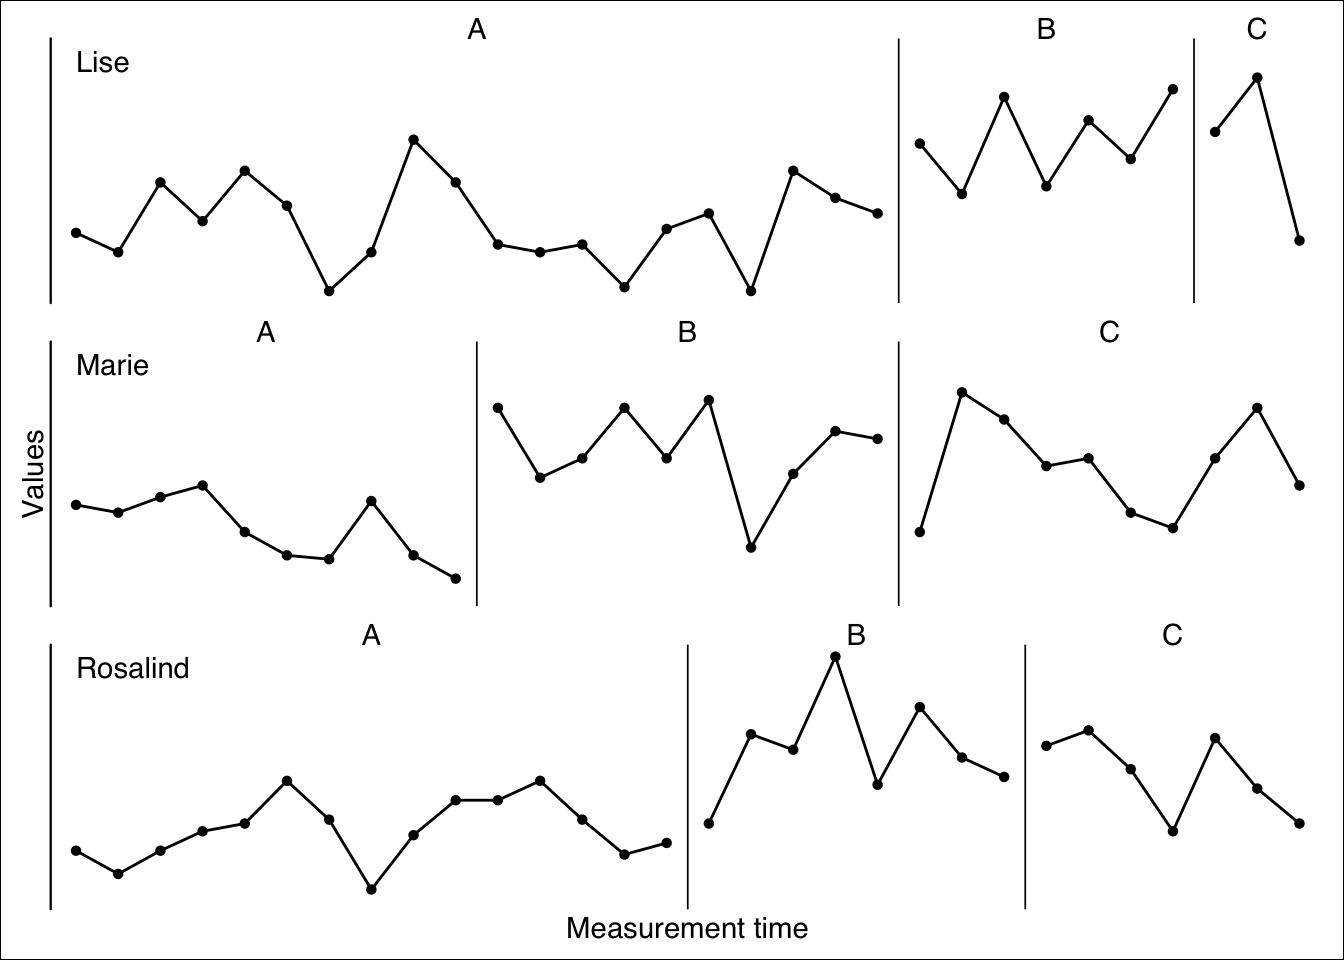
\includegraphics{./ch_scplot_files/figure-pdf/theme4-1.pdf}

}

\end{figure}

\hypertarget{theme-dark}{%
\subsection{Theme `dark'}\label{theme-dark}}

\begin{Shaded}
\begin{Highlighting}[]
\FunctionTok{scplot}\NormalTok{(exampleABC) }\SpecialCharTok{\%\textgreater{}\%}
  \FunctionTok{add\_theme}\NormalTok{(}\StringTok{"dark"}\NormalTok{)}
\end{Highlighting}
\end{Shaded}

\begin{figure}[H]

{\centering 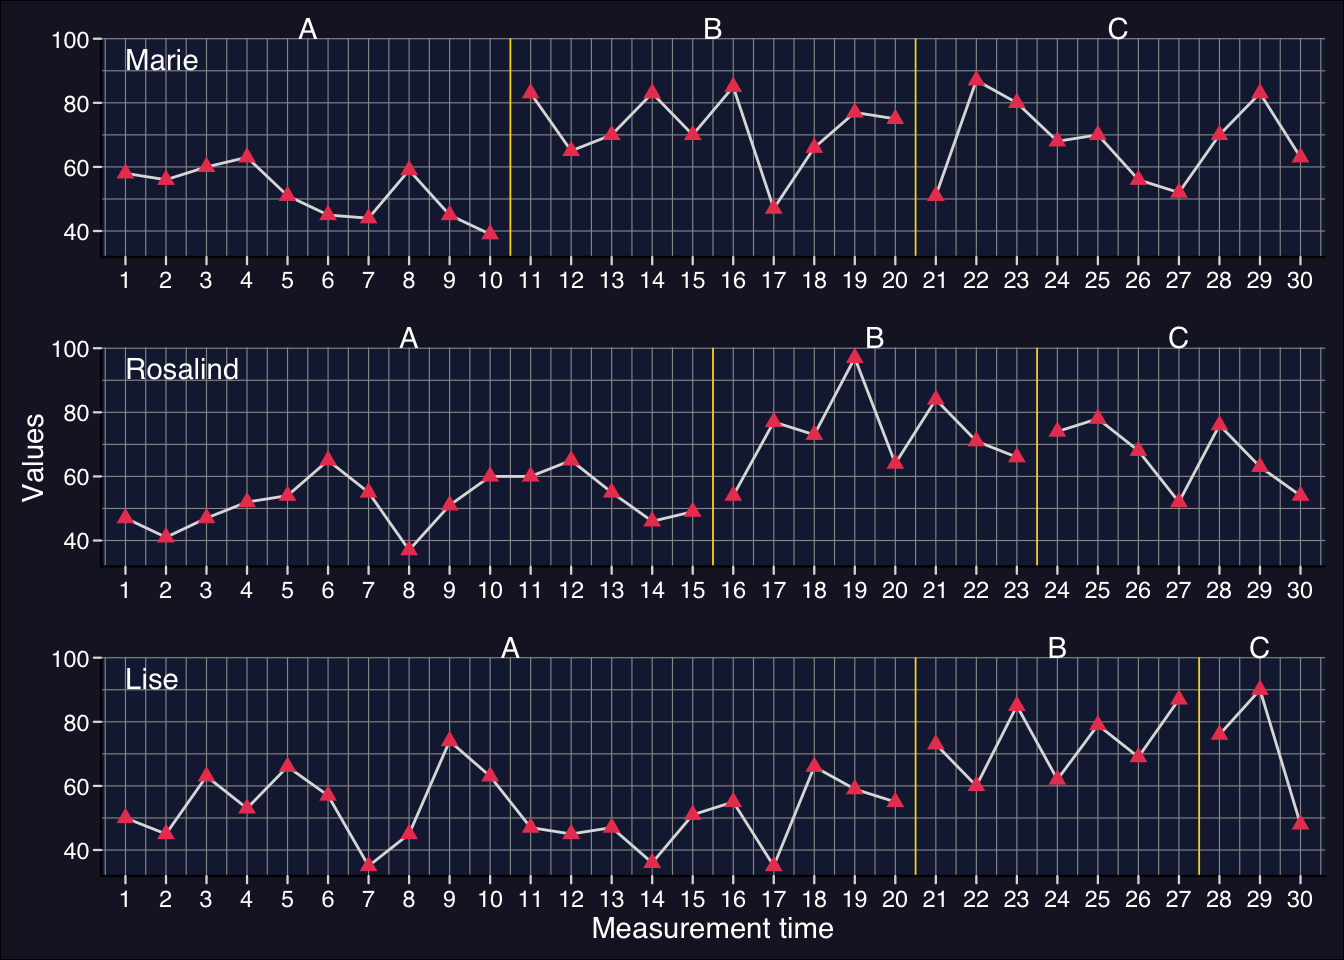
\includegraphics{./ch_scplot_files/figure-pdf/theme5-1.pdf}

}

\end{figure}

\hypertarget{theme-sienna}{%
\subsection{Theme `sienna'}\label{theme-sienna}}

\begin{Shaded}
\begin{Highlighting}[]
\FunctionTok{scplot}\NormalTok{(exampleABC) }\SpecialCharTok{\%\textgreater{}\%}
  \FunctionTok{add\_theme}\NormalTok{(}\StringTok{"sienna"}\NormalTok{)}
\end{Highlighting}
\end{Shaded}

\begin{figure}[H]

{\centering 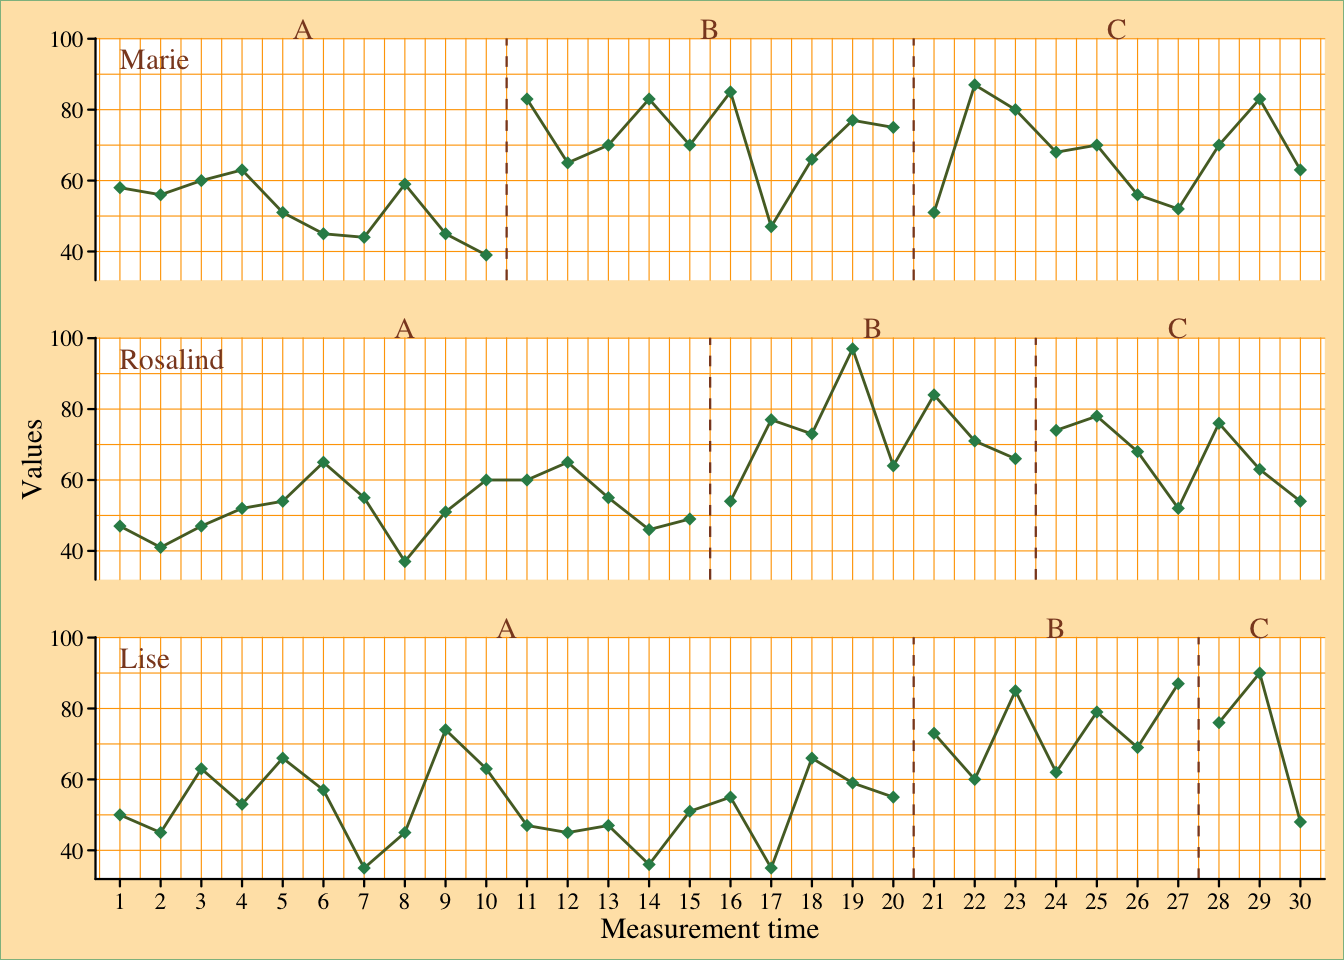
\includegraphics{./ch_scplot_files/figure-pdf/theme6-1.pdf}

}

\end{figure}

\hypertarget{combine-themes}{%
\subsection{Combine themes}\label{combine-themes}}

When providing multiple themes the order is important as the latter
overwrites styles of the former.

\begin{Shaded}
\begin{Highlighting}[]
\FunctionTok{scplot}\NormalTok{(exampleABC) }\SpecialCharTok{\%\textgreater{}\%}
  \FunctionTok{add\_theme}\NormalTok{(}\StringTok{"sienna"}\NormalTok{, }\StringTok{"minimal"}\NormalTok{, }\StringTok{"small"}\NormalTok{)}
\end{Highlighting}
\end{Shaded}

\begin{figure}[H]

{\centering 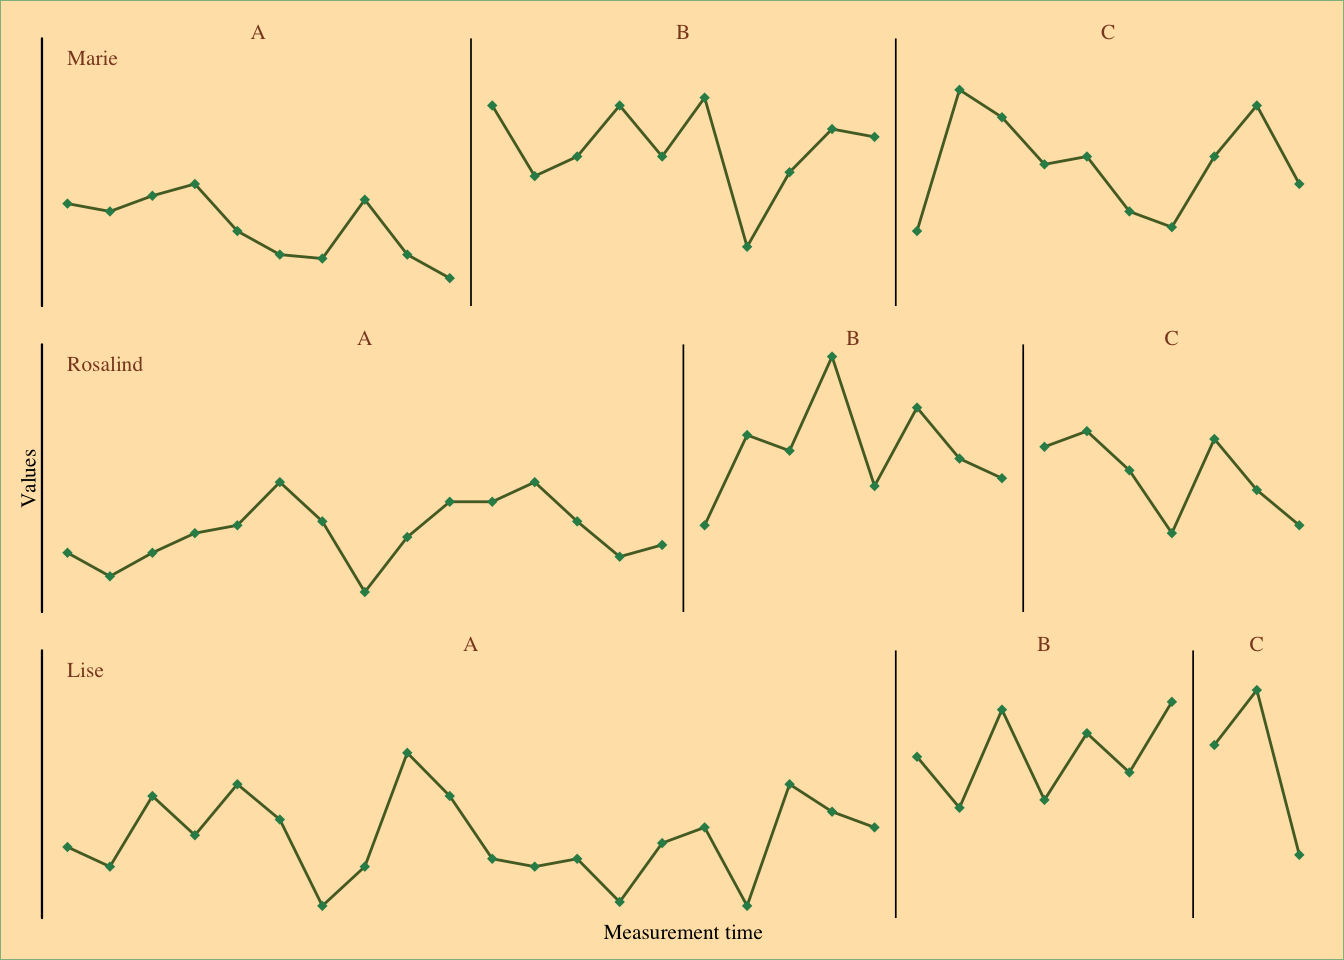
\includegraphics{./ch_scplot_files/figure-pdf/theme7-1.pdf}

}

\end{figure}

\hypertarget{set-base-text}{%
\subsection{Set base text}\label{set-base-text}}

The base text size is the absolute size. All other text sizes are
relative to this base text size.

\begin{Shaded}
\begin{Highlighting}[]
\FunctionTok{scplot}\NormalTok{(exampleAB\_decreasing}\SpecialCharTok{$}\NormalTok{Peter) }\SpecialCharTok{\%\textgreater{}\%}
  \FunctionTok{set\_base\_text}\NormalTok{(}\AttributeTok{colour =} \StringTok{"blue"}\NormalTok{, }\AttributeTok{family =} \StringTok{"serif"}\NormalTok{, }\AttributeTok{face =} \StringTok{"italic"}\NormalTok{, }\AttributeTok{size =} \DecValTok{14}\NormalTok{)}
\end{Highlighting}
\end{Shaded}

\begin{figure}[H]

{\centering 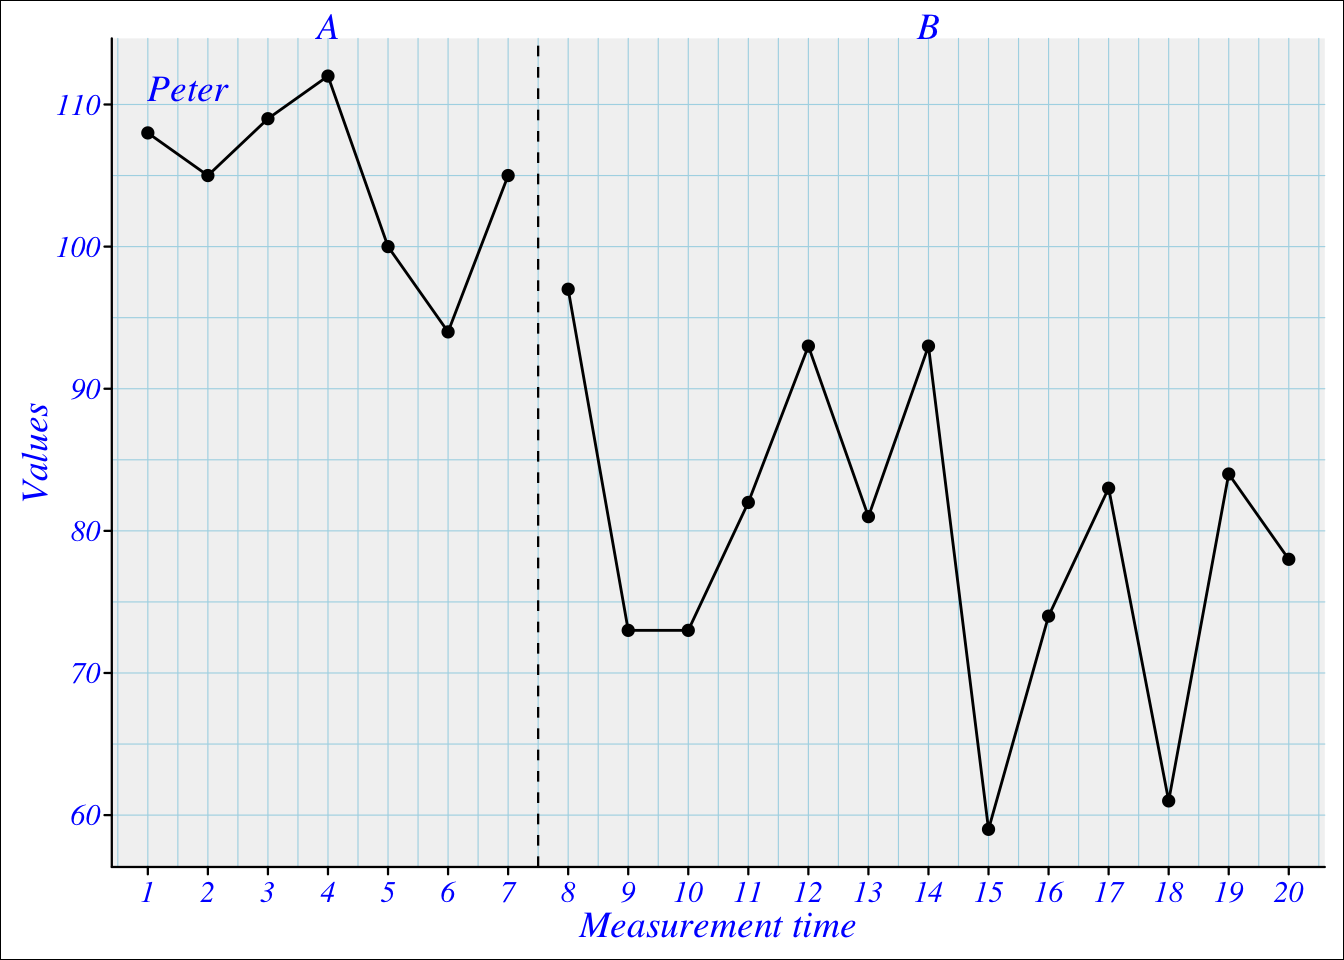
\includegraphics{./ch_scplot_files/figure-pdf/base1-1.pdf}

}

\end{figure}

\hypertarget{add-title-and-caption}{%
\section{Add title and caption}\label{add-title-and-caption}}

\begin{Shaded}
\begin{Highlighting}[]
\FunctionTok{scplot}\NormalTok{(exampleAB\_decreasing) }\SpecialCharTok{\%\textgreater{}\%}
  \FunctionTok{add\_title}\NormalTok{(}\StringTok{"A new plot"}\NormalTok{, }\AttributeTok{color =} \StringTok{"darkblue"}\NormalTok{, }\AttributeTok{size =} \FloatTok{1.3}\NormalTok{) }\SpecialCharTok{\%\textgreater{}\%}
  \FunctionTok{add\_caption}\NormalTok{(}\StringTok{"Note. What a nice plot!"}\NormalTok{, }\AttributeTok{face =} \StringTok{"italic"}\NormalTok{, }\AttributeTok{colour =} \StringTok{"darkred"}\NormalTok{)}
\end{Highlighting}
\end{Shaded}

\begin{figure}[H]

{\centering 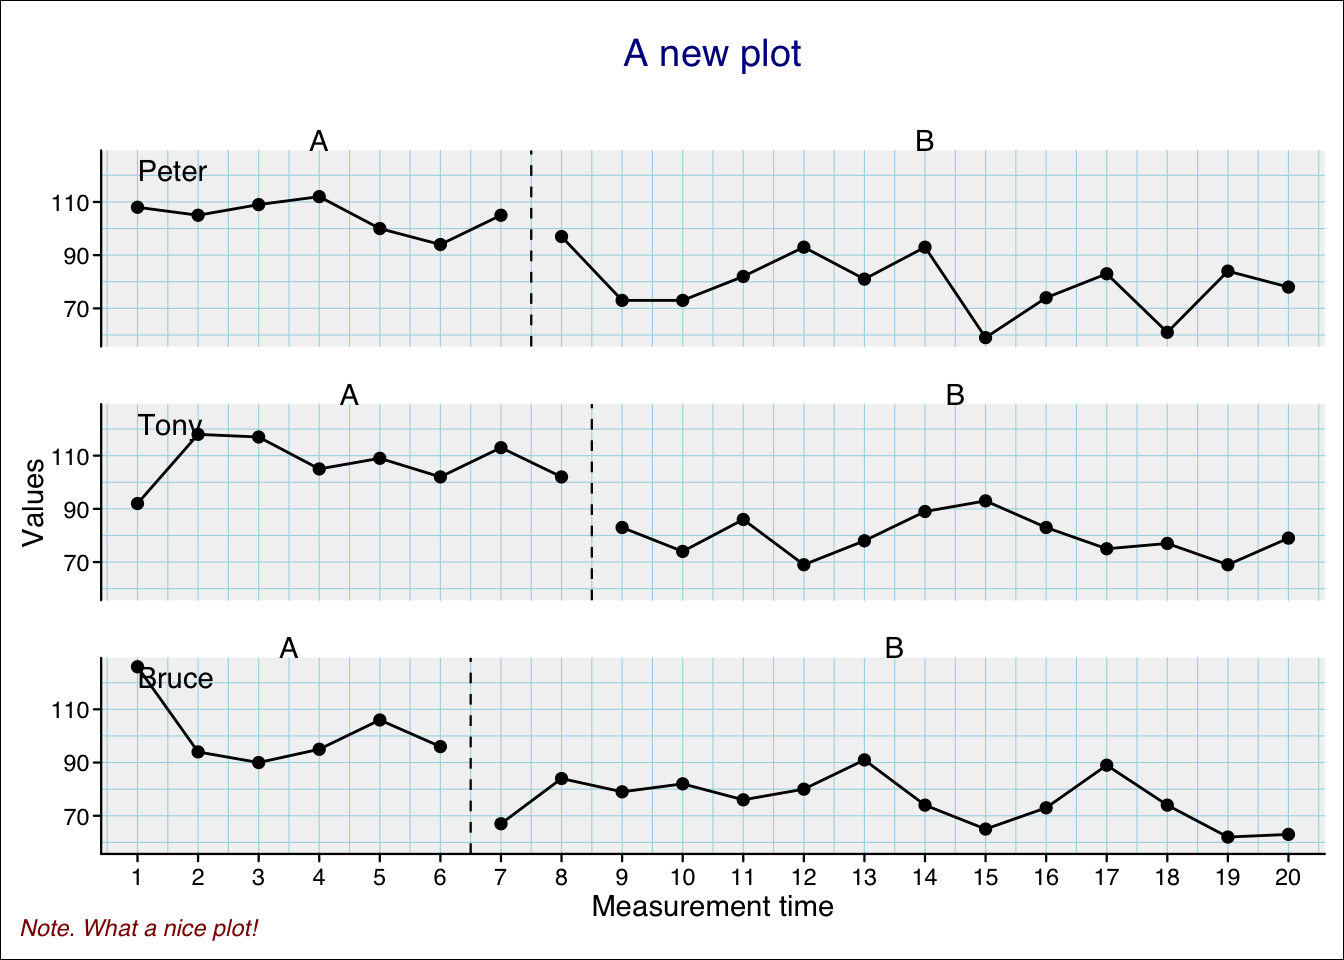
\includegraphics{./ch_scplot_files/figure-pdf/title1-1.pdf}

}

\end{figure}

\hypertarget{add-a-legend}{%
\section{Add a legend}\label{add-a-legend}}

\begin{Shaded}
\begin{Highlighting}[]
\FunctionTok{scplot}\NormalTok{(exampleABC) }\SpecialCharTok{\%\textgreater{}\%}
  \FunctionTok{add\_statline}\NormalTok{(}\StringTok{"mean"}\NormalTok{, }\AttributeTok{color =} \StringTok{"darkred"}\NormalTok{) }\SpecialCharTok{\%\textgreater{}\%}
  \FunctionTok{add\_statline}\NormalTok{(}\StringTok{"min"}\NormalTok{, }\AttributeTok{phase =} \StringTok{"B"}\NormalTok{, }\AttributeTok{size =} \FloatTok{0.2}\NormalTok{, }\AttributeTok{color =} \StringTok{"darkblue"}\NormalTok{) }\SpecialCharTok{\%\textgreater{}\%}
  \FunctionTok{add\_legend}\NormalTok{()}
\end{Highlighting}
\end{Shaded}

\begin{figure}[H]

{\centering 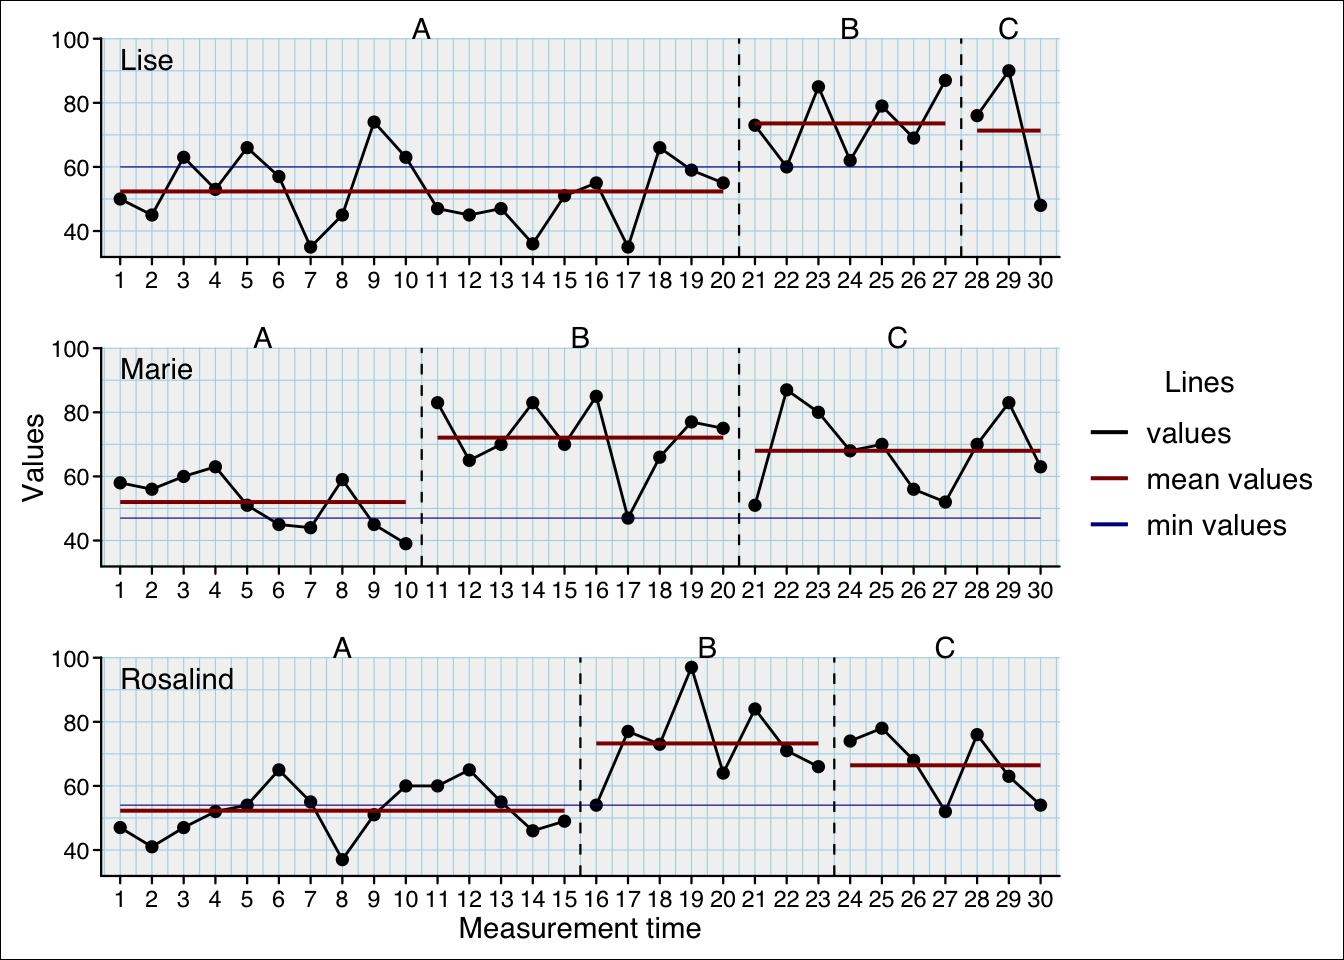
\includegraphics{./ch_scplot_files/figure-pdf/legend1-1.pdf}

}

\end{figure}

and set specific elements

\begin{Shaded}
\begin{Highlighting}[]
\FunctionTok{scplot}\NormalTok{(exampleABC) }\SpecialCharTok{\%\textgreater{}\%}
  \FunctionTok{add\_statline}\NormalTok{(}\StringTok{"mean"}\NormalTok{, }\AttributeTok{color =} \StringTok{"darkred"}\NormalTok{) }\SpecialCharTok{\%\textgreater{}\%}
  \FunctionTok{add\_legend}\NormalTok{(}
    \AttributeTok{position =} \StringTok{"left"}\NormalTok{, }
    \AttributeTok{title =} \FunctionTok{list}\NormalTok{(}\AttributeTok{size =} \DecValTok{12}\NormalTok{, }\AttributeTok{face =} \StringTok{"italic"}\NormalTok{),}
    \AttributeTok{background =} \FunctionTok{list}\NormalTok{(}\AttributeTok{fill =} \StringTok{"grey95"}\NormalTok{, }\AttributeTok{colour =} \StringTok{"black"}\NormalTok{)}
\NormalTok{  )}
\end{Highlighting}
\end{Shaded}

\begin{figure}[H]

{\centering 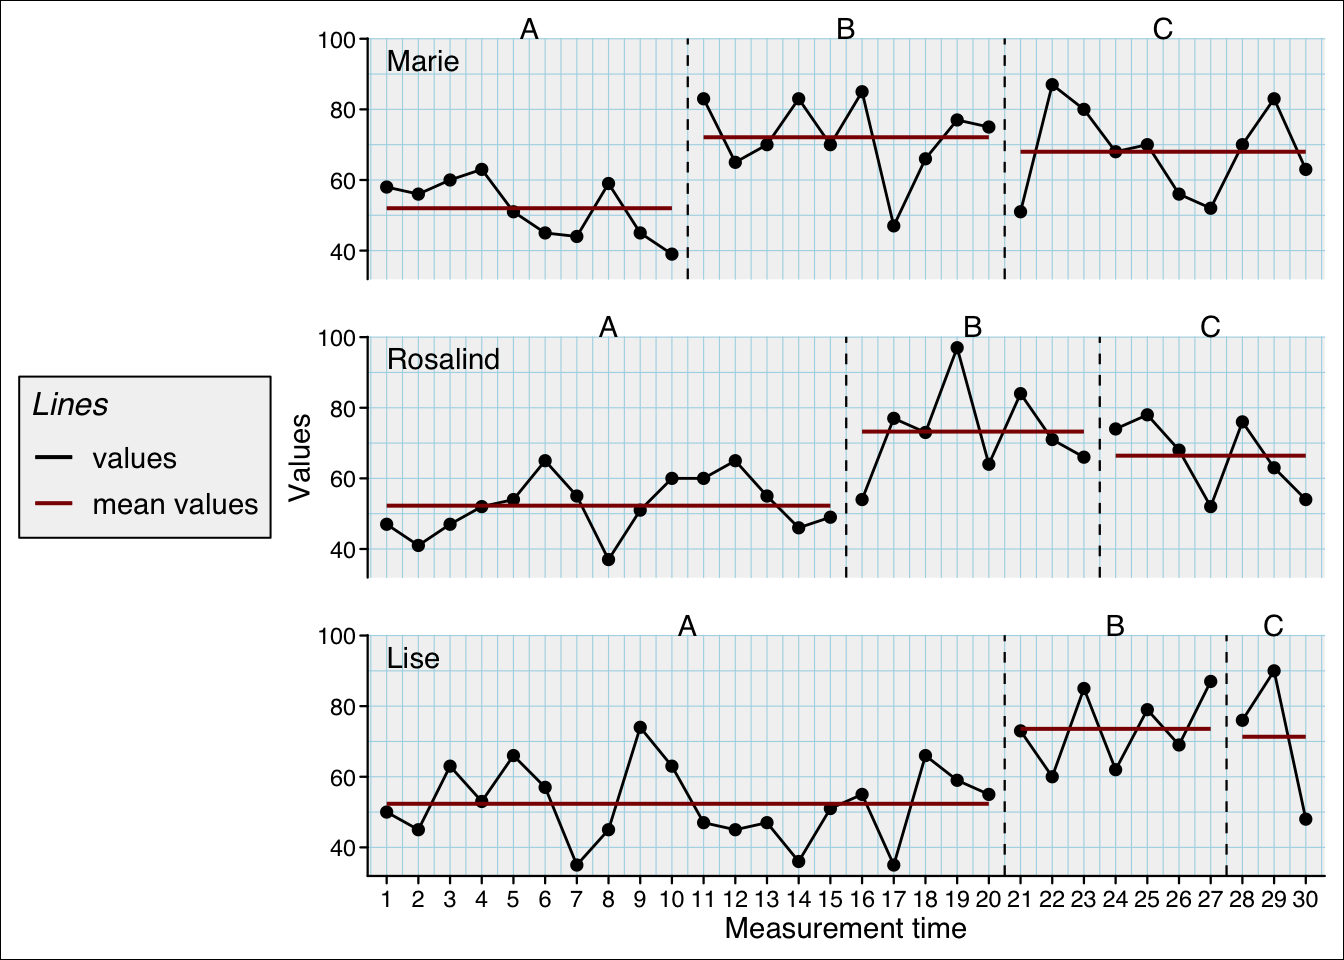
\includegraphics{./ch_scplot_files/figure-pdf/legend2-1.pdf}

}

\end{figure}

\hypertarget{customize-axis-settings}{%
\section{Customize axis settings}\label{customize-axis-settings}}

When axis ticks are to close together set the increment argument to
leave additional space (e.g.~\texttt{increment\ =\ 2} will annotate
every other value). When you set \texttt{increment\_from\ =\ 0} an
additional tick will be set at 1 although counting of the increments
will start at 0.

\begin{Shaded}
\begin{Highlighting}[]
\FunctionTok{scplot}\NormalTok{(exampleA1B1A2B2) }\SpecialCharTok{\%\textgreater{}\%} 
  \FunctionTok{set\_xaxis}\NormalTok{(}\AttributeTok{increment\_from =} \DecValTok{0}\NormalTok{, }\AttributeTok{increment =} \DecValTok{5}\NormalTok{, }
            \AttributeTok{color =} \StringTok{"darkred"}\NormalTok{, }\AttributeTok{size =} \FloatTok{0.7}\NormalTok{, }\AttributeTok{angle =} \SpecialCharTok{{-}}\DecValTok{90}\NormalTok{) }\SpecialCharTok{\%\textgreater{}\%}
  \FunctionTok{set\_yaxis}\NormalTok{(}\AttributeTok{limits =} \FunctionTok{c}\NormalTok{(}\DecValTok{0}\NormalTok{, }\DecValTok{50}\NormalTok{), }\AttributeTok{size =} \FloatTok{0.7}\NormalTok{, }\AttributeTok{color =} \StringTok{"darkred"}\NormalTok{) }
\end{Highlighting}
\end{Shaded}

\begin{figure}[H]

{\centering 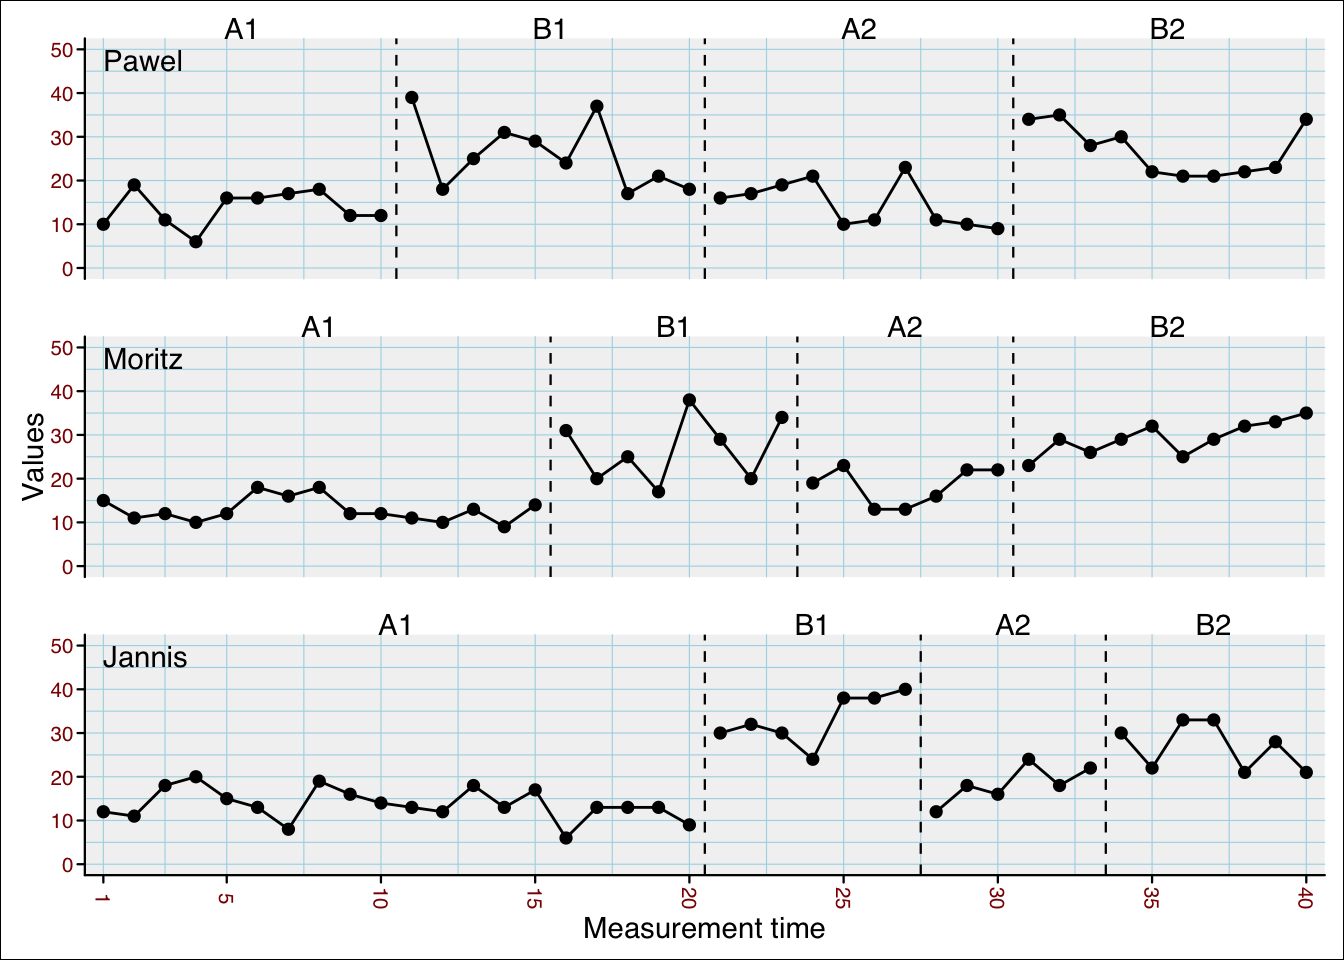
\includegraphics{./ch_scplot_files/figure-pdf/axis1-1.pdf}

}

\end{figure}

\hypertarget{customize-axis-labels}{%
\section{Customize axis labels}\label{customize-axis-labels}}

\begin{Shaded}
\begin{Highlighting}[]
\FunctionTok{scplot}\NormalTok{(exampleA1B1A2B2) }\SpecialCharTok{\%\textgreater{}\%} 
  \FunctionTok{set\_ylabel}\NormalTok{(}\StringTok{"Score"}\NormalTok{, }\AttributeTok{color =} \StringTok{"darkred"}\NormalTok{, }\AttributeTok{angle =} \DecValTok{0}\NormalTok{) }\SpecialCharTok{\%\textgreater{}\%}
  \FunctionTok{set\_xlabel}\NormalTok{(}\StringTok{"Session"}\NormalTok{, }\AttributeTok{color =} \StringTok{"darkred"}\NormalTok{)}
\end{Highlighting}
\end{Shaded}

\begin{figure}[H]

{\centering 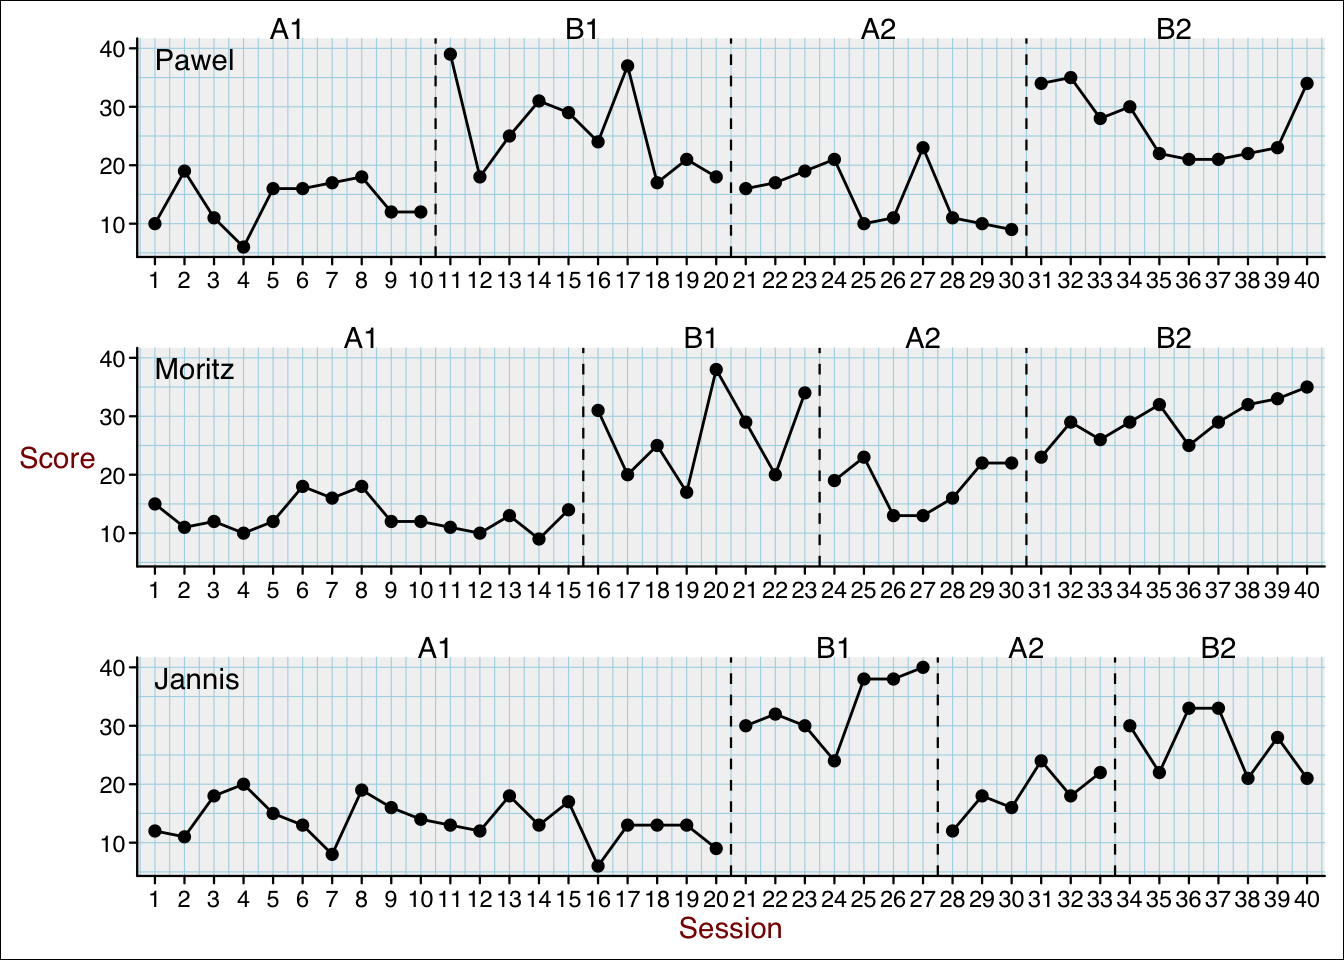
\includegraphics{./ch_scplot_files/figure-pdf/axis2-1.pdf}

}

\end{figure}

\hypertarget{change-casenames}{%
\section{Change Casenames}\label{change-casenames}}

\begin{Shaded}
\begin{Highlighting}[]
\FunctionTok{scplot}\NormalTok{(exampleA1B1A2B2) }\SpecialCharTok{\%\textgreater{}\%}
  \FunctionTok{set\_casenames}\NormalTok{(}\FunctionTok{c}\NormalTok{(}\StringTok{"A"}\NormalTok{, }\StringTok{"B"}\NormalTok{, }\StringTok{"C"}\NormalTok{), }\AttributeTok{color =} \StringTok{"darkblue"}\NormalTok{, }\AttributeTok{size =} \DecValTok{1}\NormalTok{)}
\end{Highlighting}
\end{Shaded}

\begin{figure}[H]

{\centering 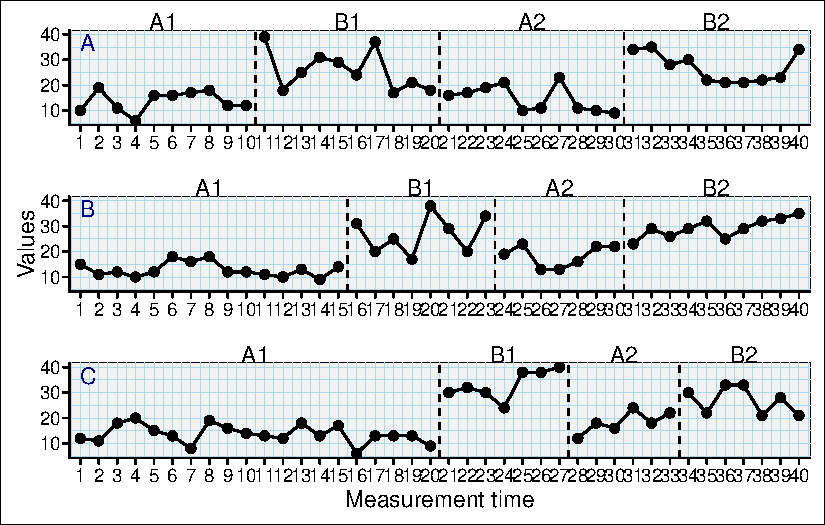
\includegraphics{./ch_scplot_files/figure-pdf/casenames1-1.pdf}

}

\end{figure}

Casenames as strips:

\begin{Shaded}
\begin{Highlighting}[]
\FunctionTok{scplot}\NormalTok{(exampleA1B1A2B2) }\SpecialCharTok{\%\textgreater{}\%}
  \FunctionTok{set\_casenames}\NormalTok{(}\AttributeTok{position =} \StringTok{"strip"}\NormalTok{, }
                \AttributeTok{background =} \FunctionTok{list}\NormalTok{(}\AttributeTok{fill =} \StringTok{"lightblue"}\NormalTok{))}
\end{Highlighting}
\end{Shaded}

\begin{figure}[H]

{\centering 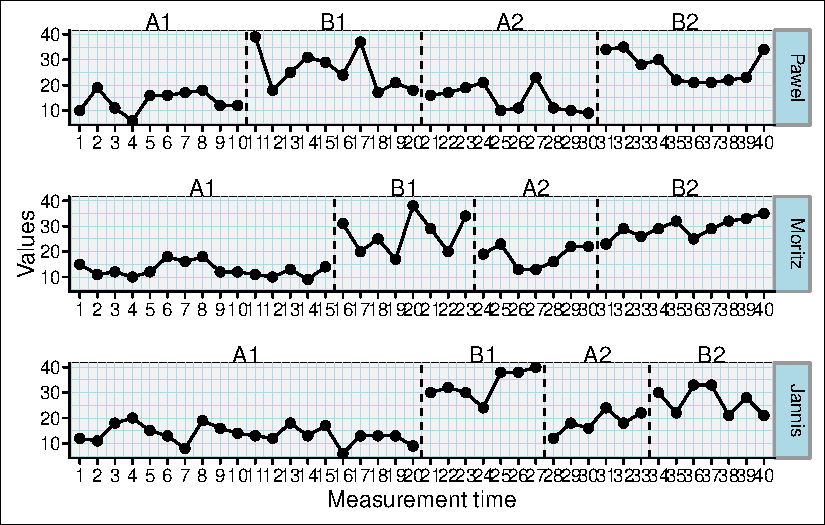
\includegraphics{./ch_scplot_files/figure-pdf/casenames2-1.pdf}

}

\end{figure}

\hypertarget{add-value-labels}{%
\section{Add value labels}\label{add-value-labels}}

\begin{Shaded}
\begin{Highlighting}[]
\FunctionTok{scplot}\NormalTok{(exampleABC) }\SpecialCharTok{\%\textgreater{}\%} 
  \FunctionTok{add\_labels}\NormalTok{(}\AttributeTok{text =} \FunctionTok{list}\NormalTok{(}\AttributeTok{color =} \StringTok{"black"}\NormalTok{, }\AttributeTok{size =} \FloatTok{0.7}\NormalTok{), }
             \AttributeTok{background =} \FunctionTok{list}\NormalTok{(}\AttributeTok{fill =} \StringTok{"grey98"}\NormalTok{), }\AttributeTok{nudge\_y =} \DecValTok{7}\NormalTok{)}
\end{Highlighting}
\end{Shaded}

\begin{verbatim}
Warning: Removed 1 rows containing missing values (geom_label).
\end{verbatim}

\begin{figure}[H]

{\centering \includegraphics{./ch_scplot_files/figure-pdf/valuelabels1-1.pdf}

}

\end{figure}

If you set the \texttt{nudge\_y} argument to 0, the label will be set
on-top the datapoints:

\begin{Shaded}
\begin{Highlighting}[]
\FunctionTok{scplot}\NormalTok{(exampleABC) }\SpecialCharTok{\%\textgreater{}\%} 
  \FunctionTok{add\_labels}\NormalTok{(}\AttributeTok{text =} \FunctionTok{list}\NormalTok{(}\AttributeTok{color =} \StringTok{"black"}\NormalTok{, }\AttributeTok{size =} \FloatTok{0.7}\NormalTok{), }
             \AttributeTok{background =} \FunctionTok{list}\NormalTok{(}\AttributeTok{fill =} \StringTok{"grey98"}\NormalTok{), }\AttributeTok{nudge\_y =} \DecValTok{0}\NormalTok{)}
\end{Highlighting}
\end{Shaded}

\begin{figure}[H]

{\centering \includegraphics{./ch_scplot_files/figure-pdf/valuelabels2-1.pdf}

}

\end{figure}

\hypertarget{add-a-ridge}{%
\section{Add a ridge}\label{add-a-ridge}}

\begin{Shaded}
\begin{Highlighting}[]
\FunctionTok{scplot}\NormalTok{(exampleAB\_mpd) }\SpecialCharTok{\%\textgreater{}\%} 
  \FunctionTok{add\_ridge}\NormalTok{(}\StringTok{"grey50"}\NormalTok{)}
\end{Highlighting}
\end{Shaded}

\begin{verbatim}
Warning in scan:::.prepare_scdf(scdf): Phase design is not identical for all
cases.
\end{verbatim}

\begin{figure}[H]

{\centering \includegraphics{./ch_scplot_files/figure-pdf/ridge1-1.pdf}

}

\end{figure}

\hypertarget{extending-scplot-with-ggplot2}{%
\section{Extending scplot with
ggplot2}\label{extending-scplot-with-ggplot2}}

\texttt{scplot()} generates ggplot2 objects. You can keep the ggplot2
object and assign it into a new object with the \texttt{as\_ggplot()}
function. Thereby, you can use many ggplot2 functions to rework your
graphics:

\begin{Shaded}
\begin{Highlighting}[]
\NormalTok{p1 }\OtherTok{\textless{}{-}} \FunctionTok{scplot}\NormalTok{(byHeart2011}\SpecialCharTok{$}\StringTok{\textasciigrave{}}\AttributeTok{Lisa (Turkish)}\StringTok{\textasciigrave{}}\NormalTok{) }\SpecialCharTok{\%\textgreater{}\%} 
        \FunctionTok{add\_theme}\NormalTok{(}\StringTok{"minimal"}\NormalTok{) }\SpecialCharTok{\%\textgreater{}\%}
        \FunctionTok{as\_ggplot}\NormalTok{()}
\NormalTok{p2 }\OtherTok{\textless{}{-}} \FunctionTok{scplot}\NormalTok{(byHeart2011}\SpecialCharTok{$}\StringTok{\textasciigrave{}}\AttributeTok{Patrick (Spanish)}\StringTok{\textasciigrave{}}\NormalTok{) }\SpecialCharTok{\%\textgreater{}\%} 
        \FunctionTok{add\_theme}\NormalTok{(}\StringTok{"minimal"}\NormalTok{) }\SpecialCharTok{\%\textgreater{}\%} 
        \FunctionTok{as\_ggplot}\NormalTok{()}
\NormalTok{p3 }\OtherTok{\textless{}{-}} \FunctionTok{scplot}\NormalTok{(byHeart2011}\SpecialCharTok{$}\StringTok{\textasciigrave{}}\AttributeTok{Anna (Twi)}\StringTok{\textasciigrave{}}\NormalTok{) }\SpecialCharTok{\%\textgreater{}\%} 
        \FunctionTok{add\_theme}\NormalTok{(}\StringTok{"minimal"}\NormalTok{) }\SpecialCharTok{\%\textgreater{}\%} 
        \FunctionTok{as\_ggplot}\NormalTok{()}
\NormalTok{p4 }\OtherTok{\textless{}{-}} \FunctionTok{scplot}\NormalTok{(byHeart2011}\SpecialCharTok{$}\StringTok{\textasciigrave{}}\AttributeTok{Melanie (Swedish)}\StringTok{\textasciigrave{}}\NormalTok{) }\SpecialCharTok{\%\textgreater{}\%} 
        \FunctionTok{add\_theme}\NormalTok{(}\StringTok{"minimal"}\NormalTok{) }\SpecialCharTok{\%\textgreater{}\%} 
        \FunctionTok{as\_ggplot}\NormalTok{()}

\FunctionTok{library}\NormalTok{(patchwork)}
\NormalTok{p1 }\SpecialCharTok{+}\NormalTok{ p2 }\SpecialCharTok{+}\NormalTok{ p3 }\SpecialCharTok{+}\NormalTok{ p4 }\SpecialCharTok{+} \FunctionTok{plot\_annotation}\NormalTok{(}\AttributeTok{tag\_levels =} \StringTok{"a"}\NormalTok{, }\AttributeTok{tag\_suffix =}  \StringTok{")"}\NormalTok{)}
\end{Highlighting}
\end{Shaded}

\begin{figure}[H]

{\centering \includegraphics{./ch_scplot_files/figure-pdf/extend1-1.pdf}

}

\end{figure}

\hypertarget{complexs-examples}{%
\section{Complexs examples}\label{complexs-examples}}

Here are some more complex examples

\begin{Shaded}
\begin{Highlighting}[]
\FunctionTok{scplot}\NormalTok{(example\_A24) }\SpecialCharTok{\%\textgreater{}\%} 
  \FunctionTok{add\_theme}\NormalTok{(}\StringTok{"default"}\NormalTok{) }\SpecialCharTok{\%\textgreater{}\%}
  \FunctionTok{add\_statline}\NormalTok{(}\StringTok{"lowess"}\NormalTok{, }\AttributeTok{color =} \StringTok{"darkred"}\NormalTok{, }\AttributeTok{size =} \FloatTok{1.5}\NormalTok{) }\SpecialCharTok{\%\textgreater{}\%}
  \FunctionTok{add\_statline}\NormalTok{(}\StringTok{"loess"}\NormalTok{, }\AttributeTok{color =} \StringTok{"red"}\NormalTok{, }\AttributeTok{size =} \FloatTok{1.5}\NormalTok{) }\SpecialCharTok{\%\textgreater{}\%}
  \FunctionTok{add\_statline}\NormalTok{(}\StringTok{"movingMean"}\NormalTok{, }\AttributeTok{lag =} \DecValTok{3}\NormalTok{, }\AttributeTok{color =} \StringTok{"lightpink"}\NormalTok{, }\AttributeTok{size =} \FloatTok{1.5}\NormalTok{) }\SpecialCharTok{\%\textgreater{}\%}
  \FunctionTok{set\_xaxis}\NormalTok{(}\AttributeTok{size =} \FloatTok{0.8}\NormalTok{, }\AttributeTok{angle =} \DecValTok{35}\NormalTok{) }\SpecialCharTok{\%\textgreater{}\%}
  \FunctionTok{set\_dataline}\NormalTok{(}\AttributeTok{point =} \StringTok{"none"}\NormalTok{) }\SpecialCharTok{\%\textgreater{}\%}
  \FunctionTok{add\_legend}\NormalTok{(}\AttributeTok{position =} \FunctionTok{c}\NormalTok{(}\FloatTok{0.8}\NormalTok{, }\FloatTok{0.75}\NormalTok{), }\AttributeTok{background =} \FunctionTok{list}\NormalTok{(}\AttributeTok{color =} \StringTok{"grey50"}\NormalTok{)) }\SpecialCharTok{\%\textgreater{}\%}
  \FunctionTok{set\_phasenames}\NormalTok{(}\FunctionTok{c}\NormalTok{(}\StringTok{"no speedlimit"}\NormalTok{, }\StringTok{"with speedlimit"}\NormalTok{), }\AttributeTok{position =} \StringTok{"left"}\NormalTok{, }
                 \AttributeTok{hjust =} \DecValTok{0}\NormalTok{, }\AttributeTok{vjust =} \DecValTok{1}\NormalTok{) }\SpecialCharTok{\%\textgreater{}\%}
  \FunctionTok{set\_casenames}\NormalTok{(}\StringTok{""}\NormalTok{) }\SpecialCharTok{\%\textgreater{}\%}
  \FunctionTok{add\_title}\NormalTok{(}\StringTok{"Effect of a speedlimit on the A24"}\NormalTok{) }\SpecialCharTok{\%\textgreater{}\%}
  \FunctionTok{add\_caption}\NormalTok{(}\StringTok{"Note: Moving mean calculated with lag three"}\NormalTok{, }\AttributeTok{face =} \DecValTok{3}\NormalTok{) }\SpecialCharTok{\%\textgreater{}\%}
  \FunctionTok{add\_ridge}\NormalTok{(}\AttributeTok{color =} \StringTok{"lightblue"}\NormalTok{)}
\end{Highlighting}
\end{Shaded}

\begin{figure}[H]

{\centering \includegraphics{./ch_scplot_files/figure-pdf/complex1-1.pdf}

}

\end{figure}

\begin{Shaded}
\begin{Highlighting}[]
\FunctionTok{scplot}\NormalTok{(exampleAB\_add) }\SpecialCharTok{\%\textgreater{}\%}
  \FunctionTok{add\_dataline}\NormalTok{(}\StringTok{"cigarrets"}\NormalTok{, }\AttributeTok{point =} \FunctionTok{list}\NormalTok{(}\AttributeTok{size =} \DecValTok{1}\NormalTok{)) }\SpecialCharTok{\%\textgreater{}\%}
  \FunctionTok{add\_statline}\NormalTok{(}\StringTok{"trend"}\NormalTok{, }\AttributeTok{linetype =} \StringTok{"dashed"}\NormalTok{) }\SpecialCharTok{\%\textgreater{}\%}
  \FunctionTok{add\_statline}\NormalTok{(}\StringTok{"mean"}\NormalTok{, }\AttributeTok{variable =} \StringTok{"cigarrets"}\NormalTok{, }\AttributeTok{color =} \StringTok{"darkred"}\NormalTok{) }\SpecialCharTok{\%\textgreater{}\%}
  \FunctionTok{add\_marks}\NormalTok{(}\AttributeTok{positions =} \FunctionTok{c}\NormalTok{(}\DecValTok{14}\NormalTok{,}\DecValTok{20}\NormalTok{), }\AttributeTok{size =} \DecValTok{3}\NormalTok{, }\AttributeTok{variable =} \StringTok{"cigarrets"}\NormalTok{)}\SpecialCharTok{\%\textgreater{}\%}
  \FunctionTok{add\_marks}\NormalTok{(}\AttributeTok{positions =} \StringTok{"cigarrets \textgreater{} quantile(cigarrets, 0.75)"}\NormalTok{, }\AttributeTok{size =} \DecValTok{3}\NormalTok{) }\SpecialCharTok{\%\textgreater{}\%}
  \FunctionTok{set\_xaxis}\NormalTok{(}\AttributeTok{increment =} \DecValTok{5}\NormalTok{) }\SpecialCharTok{\%\textgreater{}\%}
  \FunctionTok{set\_phasenames}\NormalTok{(}\AttributeTok{color =} \ConstantTok{NA}\NormalTok{) }\SpecialCharTok{\%\textgreater{}\%}
  \FunctionTok{set\_casenames}\NormalTok{(}\AttributeTok{position =} \StringTok{"strip"}\NormalTok{) }\SpecialCharTok{\%\textgreater{}\%}
  \FunctionTok{add\_legend}\NormalTok{(}
    \AttributeTok{section\_labels =} \FunctionTok{c}\NormalTok{(}\StringTok{""}\NormalTok{, }\StringTok{""}\NormalTok{),}
    \AttributeTok{labels =} \FunctionTok{c}\NormalTok{(}\ConstantTok{NA}\NormalTok{, }\ConstantTok{NA}\NormalTok{, }\StringTok{"Trend of wellbeing"}\NormalTok{, }\StringTok{"Mean of cigarrets"}\NormalTok{),}
    \AttributeTok{text =} \FunctionTok{list}\NormalTok{(}\AttributeTok{face =} \DecValTok{3}\NormalTok{)}
\NormalTok{  ) }\SpecialCharTok{\%\textgreater{}\%}
  \FunctionTok{set\_panel}\NormalTok{(}\AttributeTok{fill =} \FunctionTok{c}\NormalTok{(}\StringTok{"lightblue"}\NormalTok{, }\StringTok{"grey80"}\NormalTok{)) }\SpecialCharTok{\%\textgreater{}\%}
  \FunctionTok{add\_ridge}\NormalTok{(}\AttributeTok{color =} \StringTok{"snow"}\NormalTok{, }\AttributeTok{variable =} \StringTok{"cigarrets"}\NormalTok{) }\SpecialCharTok{\%\textgreater{}\%}
  \FunctionTok{add\_labels}\NormalTok{(}\AttributeTok{variable =} \StringTok{"cigarrets"}\NormalTok{, }\AttributeTok{nudge\_y =} \DecValTok{2}\NormalTok{, }
             \AttributeTok{text =} \FunctionTok{list}\NormalTok{(}\AttributeTok{color =} \StringTok{"blue"}\NormalTok{, }\AttributeTok{size =} \FloatTok{0.5}\NormalTok{)) }\SpecialCharTok{\%\textgreater{}\%}
  \FunctionTok{add\_labels}\NormalTok{(}\AttributeTok{nudge\_y =} \DecValTok{2}\NormalTok{, }\AttributeTok{text =} \FunctionTok{list}\NormalTok{(}\AttributeTok{color =} \StringTok{"black"}\NormalTok{, }\AttributeTok{size =} \FloatTok{0.5}\NormalTok{),}
             \AttributeTok{background =} \FunctionTok{list}\NormalTok{(}\AttributeTok{fill =} \StringTok{"white"}\NormalTok{))}
\end{Highlighting}
\end{Shaded}

\begin{verbatim}
Warning: Removed 1 rows containing missing values (geom_label).
\end{verbatim}

\begin{figure}[H]

{\centering \includegraphics{./ch_scplot_files/figure-pdf/complex2-1.pdf}

}

\end{figure}

\begin{Shaded}
\begin{Highlighting}[]
\FunctionTok{scplot}\NormalTok{(exampleA1B1A2B2) }\SpecialCharTok{\%\textgreater{}\%} 
  \FunctionTok{set\_xaxis}\NormalTok{(}\AttributeTok{increment =} \DecValTok{4}\NormalTok{, }\AttributeTok{color =} \StringTok{"brown"}\NormalTok{) }\SpecialCharTok{\%\textgreater{}\%}
  \FunctionTok{set\_yaxis}\NormalTok{(}\AttributeTok{color =} \StringTok{"sienna3"}\NormalTok{) }\SpecialCharTok{\%\textgreater{}\%}
  \FunctionTok{set\_ylabel}\NormalTok{(}\StringTok{"Points"}\NormalTok{, }\AttributeTok{color =} \StringTok{"sienna3"}\NormalTok{, }\AttributeTok{angle =} \DecValTok{0}\NormalTok{) }\SpecialCharTok{\%\textgreater{}\%}
  \FunctionTok{set\_xlabel}\NormalTok{(}\StringTok{"Weeks"}\NormalTok{, }\AttributeTok{size =} \DecValTok{1}\NormalTok{, }\AttributeTok{color =} \StringTok{"brown"}\NormalTok{) }\SpecialCharTok{\%\textgreater{}\%}
  \FunctionTok{add\_title}\NormalTok{(}\StringTok{"Points by week"}\NormalTok{, }\AttributeTok{color =} \StringTok{"sienna4"}\NormalTok{, }\AttributeTok{face =} \DecValTok{3}\NormalTok{) }\SpecialCharTok{\%\textgreater{}\%}
  \FunctionTok{add\_caption}\NormalTok{(}\StringTok{"Note: An extensive Example."}\NormalTok{,}
              \AttributeTok{color =} \StringTok{"black"}\NormalTok{, }\AttributeTok{size =} \DecValTok{1}\NormalTok{, }\AttributeTok{face =} \DecValTok{3}\NormalTok{) }\SpecialCharTok{\%\textgreater{}\%}
  \FunctionTok{set\_phasenames}\NormalTok{(}\FunctionTok{c}\NormalTok{(}\StringTok{"Baseline"}\NormalTok{, }\StringTok{"Intervention"}\NormalTok{, }\StringTok{"Fall{-}Back"}\NormalTok{, }\StringTok{"Intervention\_2"}\NormalTok{), }
                 \AttributeTok{size =} \DecValTok{0}\NormalTok{) }\SpecialCharTok{\%\textgreater{}\%}
  \FunctionTok{add\_ridge}\NormalTok{(}\FunctionTok{alpha}\NormalTok{(}\StringTok{"lightblue"}\NormalTok{, }\FloatTok{0.5}\NormalTok{)) }\SpecialCharTok{\%\textgreater{}\%}
  \FunctionTok{set\_casenames}\NormalTok{(}\AttributeTok{labels =} \FunctionTok{sample\_names}\NormalTok{(}\DecValTok{3}\NormalTok{), }\AttributeTok{color =} \StringTok{"steelblue4"}\NormalTok{, }\AttributeTok{size =} \FloatTok{0.7}\NormalTok{) }\SpecialCharTok{\%\textgreater{}\%}
  \FunctionTok{set\_panel}\NormalTok{(}\AttributeTok{fill =} \FunctionTok{c}\NormalTok{(}\StringTok{"grey80"}\NormalTok{, }\StringTok{"grey95"}\NormalTok{), }\AttributeTok{color =} \StringTok{"sienna4"}\NormalTok{) }\SpecialCharTok{\%\textgreater{}\%}
  \FunctionTok{add\_grid}\NormalTok{(}\AttributeTok{color =} \StringTok{"grey85"}\NormalTok{, }\AttributeTok{size =} \FloatTok{0.5}\NormalTok{) }\SpecialCharTok{\%\textgreater{}\%}
  \FunctionTok{set\_dataline}\NormalTok{(}\AttributeTok{size =} \FloatTok{0.5}\NormalTok{, }\AttributeTok{linetype =} \StringTok{"solid"}\NormalTok{, }
               \AttributeTok{point =} \FunctionTok{list}\NormalTok{(}\AttributeTok{colour =} \StringTok{"sienna4"}\NormalTok{, }\AttributeTok{size =} \FloatTok{0.5}\NormalTok{, }\AttributeTok{shape =} \DecValTok{18}\NormalTok{)) }\SpecialCharTok{\%\textgreater{}\%}
  \FunctionTok{add\_labels}\NormalTok{(}\AttributeTok{text =} \FunctionTok{list}\NormalTok{(}\AttributeTok{color =} \StringTok{"sienna"}\NormalTok{, }\AttributeTok{size =} \FloatTok{0.7}\NormalTok{), }\AttributeTok{nudge\_y =} \DecValTok{4}\NormalTok{) }\SpecialCharTok{\%\textgreater{}\%}
  \FunctionTok{set\_separator}\NormalTok{(}\AttributeTok{size =} \FloatTok{0.5}\NormalTok{, }\AttributeTok{linetype =} \StringTok{"solid"}\NormalTok{, }\AttributeTok{color =} \StringTok{"sienna"}\NormalTok{) }\SpecialCharTok{\%\textgreater{}\%}
  \FunctionTok{add\_statline}\NormalTok{(}\AttributeTok{stat =} \StringTok{"trendA"}\NormalTok{, }\AttributeTok{color =} \StringTok{"tomato2"}\NormalTok{) }\SpecialCharTok{\%\textgreater{}\%}
  \FunctionTok{add\_statline}\NormalTok{(}\AttributeTok{stat =} \StringTok{"max"}\NormalTok{, }\AttributeTok{phase =} \FunctionTok{c}\NormalTok{(}\DecValTok{1}\NormalTok{, }\DecValTok{3}\NormalTok{), }\AttributeTok{linetype =} \StringTok{"dashed"}\NormalTok{) }\SpecialCharTok{\%\textgreater{}\%}
  \FunctionTok{add\_marks}\NormalTok{(}\AttributeTok{case =} \DecValTok{1}\SpecialCharTok{:}\DecValTok{2}\NormalTok{, }\AttributeTok{positions =} \DecValTok{14}\NormalTok{, }\AttributeTok{color =} \StringTok{"red3"}\NormalTok{, }\AttributeTok{size =} \DecValTok{2}\NormalTok{, }\AttributeTok{shape =} \DecValTok{4}\NormalTok{) }\SpecialCharTok{\%\textgreater{}\%}
  \FunctionTok{add\_marks}\NormalTok{(}\AttributeTok{case =} \StringTok{"all"}\NormalTok{, }\AttributeTok{positions =} \StringTok{"values \textless{} quantile(values, 0.1)"}\NormalTok{, }
            \AttributeTok{color =} \StringTok{"blue3"}\NormalTok{, }\AttributeTok{size =} \FloatTok{1.5}\NormalTok{) }\SpecialCharTok{\%\textgreater{}\%}
  \FunctionTok{add\_marks}\NormalTok{(}\AttributeTok{positions =} \FunctionTok{outlier}\NormalTok{(exampleABAB), }\AttributeTok{color =} \StringTok{"brown"}\NormalTok{, }\AttributeTok{size =} \DecValTok{2}\NormalTok{) }\SpecialCharTok{\%\textgreater{}\%}
  \FunctionTok{add\_text}\NormalTok{(}\AttributeTok{case =} \DecValTok{1}\NormalTok{, }\AttributeTok{x =} \DecValTok{5}\NormalTok{, }\AttributeTok{y =} \DecValTok{35}\NormalTok{, }\AttributeTok{label =} \StringTok{"Interesting"}\NormalTok{, }
           \AttributeTok{color =} \StringTok{"darkgreen"}\NormalTok{, }\AttributeTok{angle =} \DecValTok{20}\NormalTok{, }\AttributeTok{size =} \FloatTok{0.7}\NormalTok{) }\SpecialCharTok{\%\textgreater{}\%}
  \FunctionTok{add\_arrow}\NormalTok{(}\AttributeTok{case =} \DecValTok{1}\NormalTok{, }\DecValTok{5}\NormalTok{, }\DecValTok{30}\NormalTok{, }\DecValTok{5}\NormalTok{, }\DecValTok{22}\NormalTok{, }\AttributeTok{color =} \StringTok{"steelblue"}\NormalTok{) }\SpecialCharTok{\%\textgreater{}\%}
  \FunctionTok{set\_background}\NormalTok{(}\AttributeTok{fill =} \StringTok{"white"}\NormalTok{) }\SpecialCharTok{\%\textgreater{}\%}
  \FunctionTok{add\_legend}\NormalTok{()}
\end{Highlighting}
\end{Shaded}

\begin{verbatim}
Warning: Removed 6 rows containing missing values (geom_text).
\end{verbatim}

\begin{figure}[H]

{\centering \includegraphics{./ch_scplot_files/figure-pdf/complex3-1.pdf}

}

\end{figure}

Adding bars is a bit more complicated:

\begin{itemize}
\tightlist
\item
  Set the \texttt{type} argument to \texttt{"bar"}\\
\item
  Extend the limits of the x-axis by 1 (here from \texttt{0} to
  \texttt{41})\\
\item
  Set the left margin of the x-axis to \texttt{0} with the
  \texttt{expand} argument.
\end{itemize}

\begin{Shaded}
\begin{Highlighting}[]
\FunctionTok{scplot}\NormalTok{(exampleAB\_add) }\SpecialCharTok{\%\textgreater{}\%}
  \FunctionTok{set\_xaxis}\NormalTok{(}\AttributeTok{expand =} \FunctionTok{c}\NormalTok{(}\DecValTok{0}\NormalTok{, }\DecValTok{0}\NormalTok{), }\AttributeTok{limits =} \FunctionTok{c}\NormalTok{(}\DecValTok{0}\NormalTok{, }\DecValTok{41}\NormalTok{)) }\SpecialCharTok{\%\textgreater{}\%}
  \FunctionTok{add\_dataline}\NormalTok{(}\StringTok{"cigarrets"}\NormalTok{, }\AttributeTok{type =} \StringTok{"bar"}\NormalTok{, }\AttributeTok{size =} \FloatTok{0.6}\NormalTok{, }\AttributeTok{point =} \StringTok{"none"}\NormalTok{) }\SpecialCharTok{\%\textgreater{}\%}
  \FunctionTok{add\_statline}\NormalTok{(}\StringTok{"mean"}\NormalTok{, }\AttributeTok{variable =} \StringTok{"cigarrets"}\NormalTok{, }\AttributeTok{color =} \StringTok{"darkred"}\NormalTok{) }\SpecialCharTok{\%\textgreater{}\%}
  \FunctionTok{add\_statline}\NormalTok{(}\StringTok{"trend"}\NormalTok{, }\AttributeTok{linetype =} \StringTok{"dashed"}\NormalTok{) }\SpecialCharTok{\%\textgreater{}\%}
  \FunctionTok{set\_casenames}\NormalTok{(}\AttributeTok{position =} \StringTok{"strip"}\NormalTok{)}
\end{Highlighting}
\end{Shaded}

\begin{figure}[H]

{\centering \includegraphics{./ch_scplot_files/figure-pdf/complex4-1.pdf}

}

\end{figure}

\hypertarget{references}{%
\chapter*{References}\label{references}}
\addcontentsline{toc}{chapter}{References}

\hypertarget{refs}{}
\begin{CSLReferences}{1}{0}
\leavevmode\vadjust pre{\hypertarget{ref-brossart2018a}{}}%
Brossart, D. F., Laird, V. C., \& Armstrong, T. W. (2018). Interpreting
Kendall{'}s Tau and Tau-U for single-case experimental designs.
\emph{Cogent Psychology}, \emph{5}(1), 1--26.
\url{https://doi.org/10.1080/23311908.2018.1518687}

\leavevmode\vadjust pre{\hypertarget{ref-bultuxe92008}{}}%
Bulté, I., \& Onghena, P. (2008). An r package for single-case
randomization tests. \emph{Behavior Research Methods}, \emph{40}(2),
467--478. \url{https://doi.org/10.3758/BRM.40.2.467}

\leavevmode\vadjust pre{\hypertarget{ref-bultuxe92009}{}}%
Bulté, I., \& Onghena, P. (2009). Randomization tests for
multiple-baseline designs: An extension of the SCRT-r package.
\emph{Behavior Research Methods}, \emph{41}(2), 477--485.
\url{https://doi.org/10.3758/BRM.41.2.477}

\leavevmode\vadjust pre{\hypertarget{ref-huitema_design_2000}{}}%
Huitema, B. E., \& Mckean, J. W. (2000). Design specification issues in
time-series intervention models. \emph{Educational and Psychological
Measurement}, \emph{60}(1), 38--58. Retrieved from
\url{http://epm.sagepub.com/content/60/1/38.short}

\leavevmode\vadjust pre{\hypertarget{ref-iglewicz_how_1993}{}}%
Iglewicz, B., \& Hoaglin, D. C. (1993). \emph{How to detect and handle
outliers}. Milwaukee, Wis. : ASQC Quality Press.

\leavevmode\vadjust pre{\hypertarget{ref-parker_percentage_2007}{}}%
Parker, Richard I., Hagan-Burke, S., \& Vannest, K. (2007). Percentage
of {All} {Non}-{Overlapping} {Data} ({PAND}) {An} {Alternative} to
{PND}. \emph{The Journal of Special Education}, \emph{40}(4), 194--204.
Retrieved from \url{http://sed.sagepub.com/content/40/4/194.short}

\leavevmode\vadjust pre{\hypertarget{ref-parker_improved_2009}{}}%
Parker, Richard I., \& Vannest, K. (2009). An improved effect size for
single-case research: {Nonoverlap} of all pairs. \emph{Behavior
Therapy}, \emph{40}(4), 357--367. Retrieved from
\url{http://www.sciencedirect.com/science/article/pii/S0005789408000816}

\leavevmode\vadjust pre{\hypertarget{ref-parker_effect_2011}{}}%
Parker, Richard I., Vannest, K. J., \& Davis, J. L. (2011a). Effect
{Size} in {Single}-{Case} {Research}: {A} {Review} of {Nine}
{Nonoverlap} {Techniques}. \emph{Behavior Modification}, \emph{35}(4),
303--322. \url{https://doi.org/10.1177/0145445511399147}

\leavevmode\vadjust pre{\hypertarget{ref-parker_combining_2011}{}}%
Parker, Richard I., Vannest, K. J., Davis, J. L., \& Sauber, S. B.
(2011b). Combining {Nonoverlap} and {Trend} for {Single}-{Case}
{Research}: {Tau}-{U}. \emph{Behavior Therapy}, \emph{42}(2), 284--299.
\url{https://doi.org/10.1016/j.beth.2010.08.006}

\leavevmode\vadjust pre{\hypertarget{ref-parker2011}{}}%
Parker, Richard I., Vannest, K. J., Davis, J. L., \& Sauber, S. B.
(2011c). Combining nonoverlap and trend for single-case research: Tau-u.
\emph{Behavior Therapy}, \emph{42}(2), 284--299.
\url{https://doi.org/10.1016/j.beth.2010.08.006}

\leavevmode\vadjust pre{\hypertarget{ref-pustejovsky2016}{}}%
Pustejovsky, J. E. (2016). \emph{What is tau-u?} Retrieved from
\url{https://www.jepusto.com/what-is-tau-u/}

\leavevmode\vadjust pre{\hypertarget{ref-R-base}{}}%
R Core Team. (2022). \emph{R: A language and environment for statistical
computing}. Retrieved from \url{https://www.R-project.org/}

\leavevmode\vadjust pre{\hypertarget{ref-RStudio}{}}%
RStudio Team. (2018). \emph{RStudio: Integrated development environment
for r}. Retrieved from \url{http://www.rstudio.com/}

\leavevmode\vadjust pre{\hypertarget{ref-scruggs_quantitative_1987}{}}%
Scruggs, T. E., Mastropieri, M. A., \& Casto, G. (1987). The
{Quantitative} {Synthesis} of {Single}-{Subject} {Research}
{Methodology} and {Validation}. \emph{Remedial and Special Education},
\emph{8}(2), 24--33. \url{https://doi.org/10.1177/074193258700800206}

\leavevmode\vadjust pre{\hypertarget{ref-siegelRobustRegressionUsing1982}{}}%
Siegel, A. F. (1982). Robust {Regression Using Repeated Medians}.
\emph{Biometrika}, \emph{69}(1), 242--244.
\url{https://doi.org/10.2307/2335877}

\leavevmode\vadjust pre{\hypertarget{ref-tarlowImprovedRankCorrelation2016a}{}}%
Tarlow, K. R. (2016). An {Improved Rank Correlation Effect Size
Statistic} for {Single}-{Case Designs}: Baseline {Corrected Tau}.
\emph{Behavior Modification}, \emph{41}(4), 427--467.
\url{https://doi.org/10.1177/0145445516676750}

\leavevmode\vadjust pre{\hypertarget{ref-R-scplot}{}}%
Wilbert, J. (2022). \emph{Scplot: Single-case plots for scan}.

\leavevmode\vadjust pre{\hypertarget{ref-R-scan}{}}%
Wilbert, J., \& Lueke, T. (2022). \emph{Scan: Single-case data analyses
for single and multiple baseline designs}.

\leavevmode\vadjust pre{\hypertarget{ref-wise_methods_2004}{}}%
Wise, E. A. (2004). Methods for analyzing psychotherapy outcomes: {A}
review of clinical significance, reliable change, and recommendations
for future directions. \emph{Journal of Personality Assessment},
\emph{82}(1), 50--59. Retrieved from
\url{http://www.tandfonline.com/doi/abs/10.1207/s15327752jpa8201_10}

\end{CSLReferences}

\appendix
\addcontentsline{toc}{part}{Appendices}

\hypertarget{changes}{%
\chapter{Changes}\label{changes}}

\hypertarget{single-case-studies-with-cases-of-varying-phase-design}{%
\subsection{Single-case studies with cases of varying phase
design}\label{single-case-studies-with-cases-of-varying-phase-design}}

Sometimes it is necessary to combine single-cases with different
phase-designs into one single-case study (for instance when some cases
include an extension phase and others do not). Various functions in scan
now can handle such a data structure.

\hypertarget{piping}{%
\subsection{Piping}\label{piping}}

The concept of piping is great for writing clean and intelligible code
that is easier to debug. We imported the pipe function
\texttt{\%\textgreater{}\%} from the \texttt{magrittr} package. Since
version 4.1, R has its own pipe operator implementation
\texttt{\textbar{}\textgreater{}}. This is great and works fine with the
\texttt{scan} package. But since the \texttt{\textbar{}\textgreater{}}
Operator is not backwards compatible for R prior versions 4.1, we will
stick with the \texttt{\%\textgreater{}\%} for a while.

To allow for smooth ``piping'' we began adding some functions
\texttt{select\_phases}, \texttt{subset}, \texttt{select\_cases},
\texttt{set\_var}, \texttt{set\_dvar}, \texttt{set\_mvar},
\texttt{set\_pvar}, and \texttt{add\_l2}.

\hypertarget{important-changes-with-version-0.50}{%
\section{Important changes with version
0.50}\label{important-changes-with-version-0.50}}

\hypertarget{new-function-names}{%
\subsection{New function names}\label{new-function-names}}

With version 0.50 scan introduced new names for its functions. The old
function names are still usable but they will return a ``deprecated''
warning telling you to use the new function names.

(\textbf{rtbl-aliases?}) shows the changes.

\hypertarget{tbl-aliases}{}
\begin{longtable}[]{@{}ll@{}}
\caption{\label{tbl-aliases}Scan previous and current function
names}\tabularnewline
\toprule()
Current function name & Previous function name \\
\midrule()
\endfirsthead
\toprule()
Current function name & Previous function name \\
\midrule()
\endhead
autocorr & autocorrSC \\
corrected\_tau & corrected\_tauSC \\
describe {[}since v0.52{]} & describeSC \\
fill\_missing & fillmissingSC \\
outlier & outlierSC \\
overlap & overlapSC \\
power\_test & power\_testSC \\
rand\_test & randSC; rand.test \\
ranks & rankSC \\
rci & rCi; rciSC \\
shift & shiftSC \\
smooth\_cases & smoothSC \\
style\_plot & style.plotSC; style\_plotSC \\
tau\_u & tauUSC \\
trend & trendSC \\
truncate\_phase & truncateSC \\
\bottomrule()
\end{longtable}

\hypertarget{change-target-variables-in-functions}{%
\subsection{Change target variables in
functions}\label{change-target-variables-in-functions}}

All functions in R that analyze data now allow for temporarily changing
dependent, phase, and measurement-time variables by adding three
argument:

\texttt{dvar} sets the dependent variable.\\
\texttt{pvar} sets the phase variable.\\
\texttt{mvar} sets the measurement-time variable.

For example, \texttt{overlap(exampleAB\_add,\ dvar\ =\ "depression")}
will report overlap parameters for the variable \emph{depression} while
\texttt{overlap(exampleAB\_add)} while take \emph{wellbeing} as the
dependent variable (as defined in the scdf).

After finishing the analysis, the variables are set back to their
original values as defined in the scdf.

\hypertarget{about-the-author}{%
\chapter{About the author}\label{about-the-author}}

\includegraphics{./images/wilbert3.jpg}

Currently, I am a professor for research methods and diagnostics at the
department of inclusive education at the University of Potsdam in
Germany. I studied education sciences at the University of Cologne where
I also did my PhD in psychology. Thereafter, I got a tenured position as
a senior researcher at the department of special education (also
University of Cologne). Later I did my habilitation on ``Pedagogic and
psychology in learning disabilities'' at the \emph{Carl von Ossietzky
University} Oldenburg.

My current work focuses on:

\begin{itemize}
\tightlist
\item
  Single-case research designs, analyzing single case data, and
  reporting single-case based results.
\item
  Social inclusion and social participation in classrooms.
\item
  Implementation of Open Science and Data Science concepts into special
  education research.
\end{itemize}

You can find more information about me on my homepage:

\url{https://jazznbass.github.io/homepage/}



\end{document}
